% Options for packages loaded elsewhere
\PassOptionsToPackage{unicode}{hyperref}
\PassOptionsToPackage{hyphens}{url}
\PassOptionsToPackage{dvipsnames,svgnames*,x11names*}{xcolor}
%
\documentclass[
  12pt,
]{book}
\usepackage{lmodern}
\usepackage{amssymb,amsmath}
\usepackage{ifxetex,ifluatex}
\ifnum 0\ifxetex 1\fi\ifluatex 1\fi=0 % if pdftex
  \usepackage[T1]{fontenc}
  \usepackage[utf8]{inputenc}
  \usepackage{textcomp} % provide euro and other symbols
\else % if luatex or xetex
  \usepackage{unicode-math}
  \defaultfontfeatures{Scale=MatchLowercase}
  \defaultfontfeatures[\rmfamily]{Ligatures=TeX,Scale=1}
  \setmonofont[]{Source Code Pro}
\fi
% Use upquote if available, for straight quotes in verbatim environments
\IfFileExists{upquote.sty}{\usepackage{upquote}}{}
\IfFileExists{microtype.sty}{% use microtype if available
  \usepackage[]{microtype}
  \UseMicrotypeSet[protrusion]{basicmath} % disable protrusion for tt fonts
}{}
\makeatletter
\@ifundefined{KOMAClassName}{% if non-KOMA class
  \IfFileExists{parskip.sty}{%
    \usepackage{parskip}
  }{% else
    \setlength{\parindent}{0pt}
    \setlength{\parskip}{6pt plus 2pt minus 1pt}}
}{% if KOMA class
  \KOMAoptions{parskip=half}}
\makeatother
\usepackage{xcolor}
\IfFileExists{xurl.sty}{\usepackage{xurl}}{} % add URL line breaks if available
\IfFileExists{bookmark.sty}{\usepackage{bookmark}}{\usepackage{hyperref}}
\hypersetup{
  pdftitle={Notas Curso de Estadística},
  pdfauthor={Maikol Solís},
  colorlinks=true,
  linkcolor=Maroon,
  filecolor=Maroon,
  citecolor=Blue,
  urlcolor=Blue,
  pdfcreator={LaTeX via pandoc}}
\urlstyle{same} % disable monospaced font for URLs
\usepackage{color}
\usepackage{fancyvrb}
\newcommand{\VerbBar}{|}
\newcommand{\VERB}{\Verb[commandchars=\\\{\}]}
\DefineVerbatimEnvironment{Highlighting}{Verbatim}{commandchars=\\\{\}}
% Add ',fontsize=\small' for more characters per line
\usepackage{framed}
\definecolor{shadecolor}{RGB}{248,248,248}
\newenvironment{Shaded}{\begin{snugshade}}{\end{snugshade}}
\newcommand{\AlertTok}[1]{\textcolor[rgb]{0.94,0.16,0.16}{#1}}
\newcommand{\AnnotationTok}[1]{\textcolor[rgb]{0.56,0.35,0.01}{\textbf{\textit{#1}}}}
\newcommand{\AttributeTok}[1]{\textcolor[rgb]{0.77,0.63,0.00}{#1}}
\newcommand{\BaseNTok}[1]{\textcolor[rgb]{0.00,0.00,0.81}{#1}}
\newcommand{\BuiltInTok}[1]{#1}
\newcommand{\CharTok}[1]{\textcolor[rgb]{0.31,0.60,0.02}{#1}}
\newcommand{\CommentTok}[1]{\textcolor[rgb]{0.56,0.35,0.01}{\textit{#1}}}
\newcommand{\CommentVarTok}[1]{\textcolor[rgb]{0.56,0.35,0.01}{\textbf{\textit{#1}}}}
\newcommand{\ConstantTok}[1]{\textcolor[rgb]{0.00,0.00,0.00}{#1}}
\newcommand{\ControlFlowTok}[1]{\textcolor[rgb]{0.13,0.29,0.53}{\textbf{#1}}}
\newcommand{\DataTypeTok}[1]{\textcolor[rgb]{0.13,0.29,0.53}{#1}}
\newcommand{\DecValTok}[1]{\textcolor[rgb]{0.00,0.00,0.81}{#1}}
\newcommand{\DocumentationTok}[1]{\textcolor[rgb]{0.56,0.35,0.01}{\textbf{\textit{#1}}}}
\newcommand{\ErrorTok}[1]{\textcolor[rgb]{0.64,0.00,0.00}{\textbf{#1}}}
\newcommand{\ExtensionTok}[1]{#1}
\newcommand{\FloatTok}[1]{\textcolor[rgb]{0.00,0.00,0.81}{#1}}
\newcommand{\FunctionTok}[1]{\textcolor[rgb]{0.00,0.00,0.00}{#1}}
\newcommand{\ImportTok}[1]{#1}
\newcommand{\InformationTok}[1]{\textcolor[rgb]{0.56,0.35,0.01}{\textbf{\textit{#1}}}}
\newcommand{\KeywordTok}[1]{\textcolor[rgb]{0.13,0.29,0.53}{\textbf{#1}}}
\newcommand{\NormalTok}[1]{#1}
\newcommand{\OperatorTok}[1]{\textcolor[rgb]{0.81,0.36,0.00}{\textbf{#1}}}
\newcommand{\OtherTok}[1]{\textcolor[rgb]{0.56,0.35,0.01}{#1}}
\newcommand{\PreprocessorTok}[1]{\textcolor[rgb]{0.56,0.35,0.01}{\textit{#1}}}
\newcommand{\RegionMarkerTok}[1]{#1}
\newcommand{\SpecialCharTok}[1]{\textcolor[rgb]{0.00,0.00,0.00}{#1}}
\newcommand{\SpecialStringTok}[1]{\textcolor[rgb]{0.31,0.60,0.02}{#1}}
\newcommand{\StringTok}[1]{\textcolor[rgb]{0.31,0.60,0.02}{#1}}
\newcommand{\VariableTok}[1]{\textcolor[rgb]{0.00,0.00,0.00}{#1}}
\newcommand{\VerbatimStringTok}[1]{\textcolor[rgb]{0.31,0.60,0.02}{#1}}
\newcommand{\WarningTok}[1]{\textcolor[rgb]{0.56,0.35,0.01}{\textbf{\textit{#1}}}}
\usepackage{longtable,booktabs}
% Correct order of tables after \paragraph or \subparagraph
\usepackage{etoolbox}
\makeatletter
\patchcmd\longtable{\par}{\if@noskipsec\mbox{}\fi\par}{}{}
\makeatother
% Allow footnotes in longtable head/foot
\IfFileExists{footnotehyper.sty}{\usepackage{footnotehyper}}{\usepackage{footnote}}
\makesavenoteenv{longtable}
\usepackage{graphicx,grffile}
\makeatletter
\def\maxwidth{\ifdim\Gin@nat@width>\linewidth\linewidth\else\Gin@nat@width\fi}
\def\maxheight{\ifdim\Gin@nat@height>\textheight\textheight\else\Gin@nat@height\fi}
\makeatother
% Scale images if necessary, so that they will not overflow the page
% margins by default, and it is still possible to overwrite the defaults
% using explicit options in \includegraphics[width, height, ...]{}
\setkeys{Gin}{width=\maxwidth,height=\maxheight,keepaspectratio}
% Set default figure placement to htbp
\makeatletter
\def\fps@figure{htbp}
\makeatother
\setlength{\emergencystretch}{3em} % prevent overfull lines
\providecommand{\tightlist}{%
  \setlength{\itemsep}{0pt}\setlength{\parskip}{0pt}}
\setcounter{secnumdepth}{5}
%\usepackage{inputenc}
% \usepackage{newpxtext,newpxmath}
\setcounter{tocdepth}{3}
\setcounter{secnumdepth}{3}
\usepackage[spanish]{babel}
\usepackage{booktabs}
\usepackage{csquotes}
\usepackage{amsmath, amsthm, amssymb,amsbsy}
\usepackage{mathtools}
\usepackage{graphics, graphicx}

% \usepackage{setspace}
% \doublespacing
%\addbibresource{bibliografia.bib}


% \usepackage{tcolorbox}
% \tcbuselibrary{theorems}
% \tcbuselibrary{breakable}
% 
% \newtcbtheorem[number within=section]{nota}{Nota}%
% {breakable, colback=yellow!5, colframe=yellow!40!gray,
% 	fonttitle=\bfseries}{nota}
% 
% \newtcbtheorem[number within=section,use counter
% from=nota]{cuidado}{Cuidado}%
% {breakable, colback=red!5, colframe=red!50!gray,
% 	fonttitle=\bfseries}{cuidado}
% 
% \newtcbtheorem[number within=section,use counter
% from=nota]{tarea}{Tarea}%
% {breakable, colback=blue!5, colframe=blue!35!black,
% 	fonttitle=\bfseries}{tarea}
% 
% \newtcbtheorem[number within=section,use counter
% from=nota]{solucion}{Solución}%
% {breakable, colback=gray!5, colframe=gray!35!black,
% 	fonttitle=\bfseries}{sol}
% 
% \newtcbtheorem[number within=section,use counter
% from=nota]{pregunta}{Pregunta}%
% {breakable,  colback=green!5, colframe=green!35!black,
% 	fonttitle=\bfseries}{preg}
% 
% \newtcbtheorem[number within=section,use counter
% from=nota]{ejemplo}{Ejemplo}%
% {breakable, colback=magenta!10, colframe=magenta!50!black,
% 	fonttitle=\bfseries}{ej}
% 
% \newtcbtheorem[number within=section,use counter
% from=nota]{laboratorio}{Laboratorio}%
% {breakable, colback=purple!10, colframe=purple!50!black,
% 	fonttitle=\bfseries}{lab}
%%end novalidate

%
%\usepackage{amsmath}
%\usepackage{amsthm}
%\usepackage{amssymb}
%%%% DEFINICIÓN DE ESTILOS DE TEOREMAS %%%
%\theoremstyle{definition}
%\newtheorem{definicion}{Definición}
%
%\theoremstyle{plain}
%\newtheorem{teorema}{Teorema}
%\newtheorem{lema}{Lema}
%%%%%%%%%%%%%%%%%%%%%%%%%%%%%%%%%%%%%%%%%%
\usepackage[style=authoryear,url=false,doi=false,eprint=false,isbn=false]{biblatex}
\addbibresource{bibliografia.bib}

\title{Notas Curso de Estadística}
\author{Maikol Solís}
\date{Actualizado el 16 junio, 2020}

\usepackage{amsthm}
\newtheorem{theorem}{Teorema}[chapter]
\newtheorem{lemma}{Lema}[chapter]
\newtheorem{corollary}{Corolario}[chapter]
\newtheorem{proposition}{Proposición}[chapter]
\newtheorem{conjecture}{Conjecture}[chapter]
\theoremstyle{definition}
\newtheorem{definition}{Definición}[chapter]
\theoremstyle{definition}
\newtheorem{example}{Ejemplo}[chapter]
\theoremstyle{definition}
\newtheorem{exercise}{Ejercicio}[chapter]
\theoremstyle{remark}
\newtheorem*{remark}{Nota: }
\newtheorem*{solution}{Solución}
\let\BeginKnitrBlock\begin \let\EndKnitrBlock\end
\begin{document}
\maketitle

{
\hypersetup{linkcolor=}
\setcounter{tocdepth}{4}
\tableofcontents
}
\hypertarget{introducciuxf3n}{%
\chapter{Introducción}\label{introducciuxf3n}}

\hypertarget{estimaciuxf3n-de-densidades}{%
\chapter{Estimación de densidades}\label{estimaciuxf3n-de-densidades}}

\hypertarget{histograma}{%
\section{Histograma}\label{histograma}}

El histograma es una de las estructuras básicas en estadística. Básicamente con este objeto se puede visualizar la distribución de los datos sin tener conocimiento previo de los mismos.

\hypertarget{construcciuxf3n-estaduxedstica}{%
\subsection{Construcción Estadística}\label{construcciuxf3n-estaduxedstica}}

Suponga que \(X_1,X_2, \dots ,X_n\) proviene de una distribución desconocida.

\begin{itemize}
\item
  Seleccione un origen \(x_0\) y divida la linea real en \emph{segmentos}.
  \begin{equation*}
  B_j = [x_0 +(j - 1)h,x_0 + jh) \quad j\in \mathbb{Z}
  \end{equation*}
\item
  Cuente cuántas observaciones caen en cada segmento. \(n_j\).
\end{itemize}

\begin{center}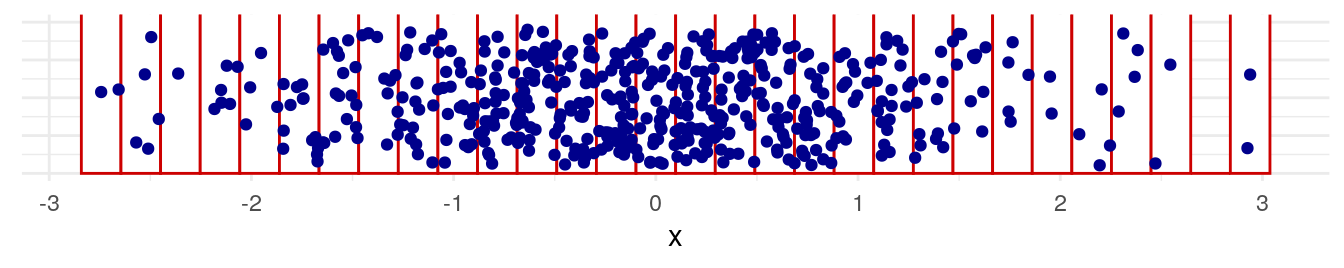
\includegraphics[width=0.7\linewidth]{Notas-Curso-Estadistica_files/figure-latex/observaciones-histograma-1} \end{center}

\begin{itemize}
\item
  Cuente la frecuencia por el tamaño de muestra \(n\) y el ancho de banda \(h\).
  \begin{equation*}
  f_j = \frac{n_j}{nh}
  \end{equation*}
\item
  Dibuje el histograma.
\end{itemize}

\begin{center}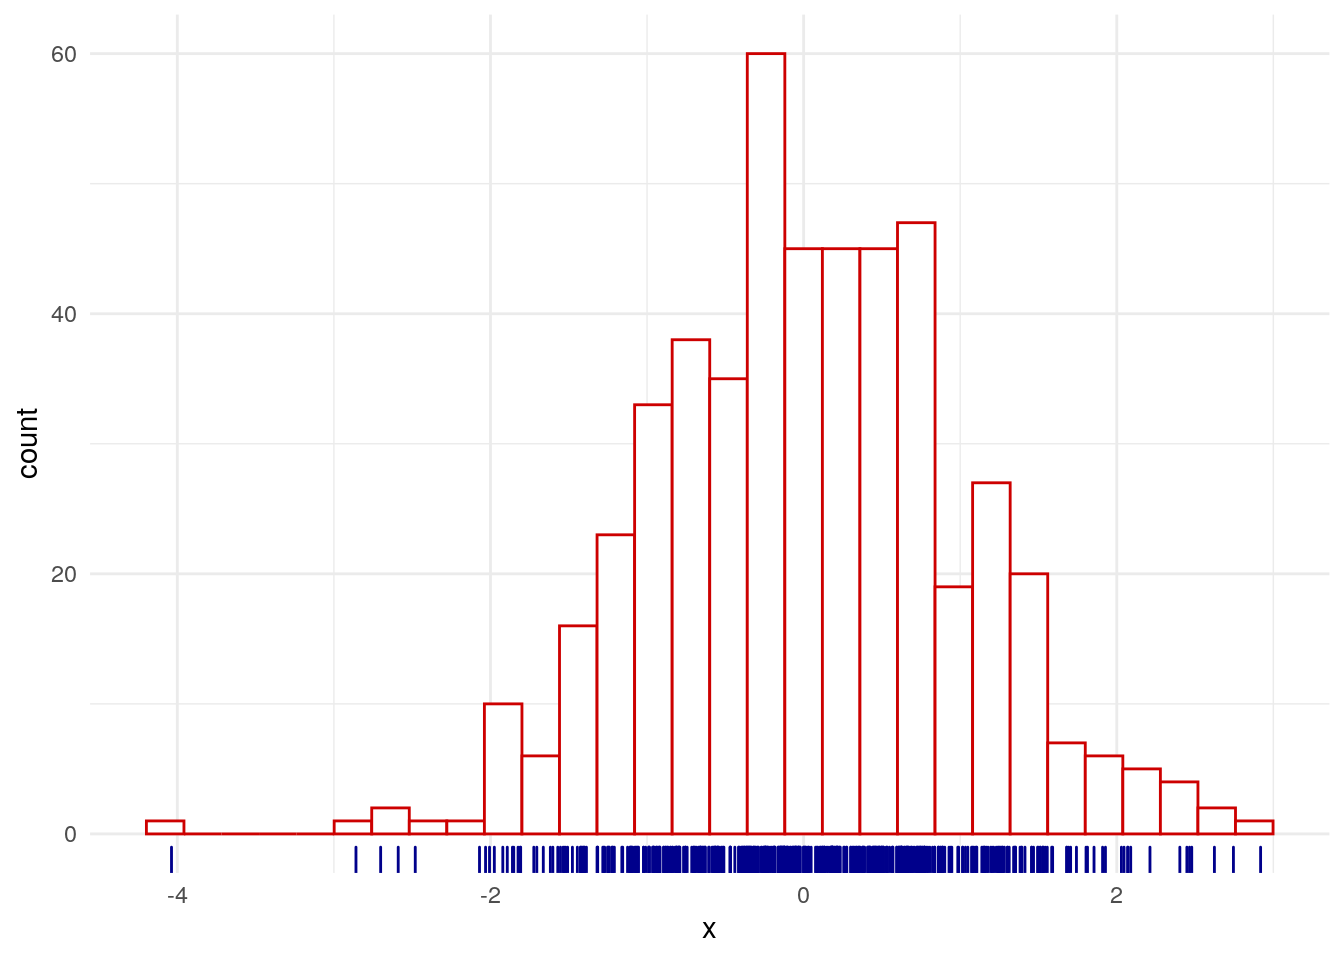
\includegraphics[width=0.7\linewidth]{Notas-Curso-Estadistica_files/figure-latex/ejemplo-inicial-histograma-1} \end{center}

Formalmente el histograma es el

\begin{equation*}
\hat{f}_h(x) = \frac{1}{nh} \sum_{i = 1}^{n} \sum_{j} I(X_i\in B_j) I(x\in B_j),
\end{equation*}

donde \(I\) es la indicadora.

\hypertarget{construcciuxf3n-probabilistica}{%
\subsection{Construcción probabilistica}\label{construcciuxf3n-probabilistica}}

Denote \(m_j=jh-h/2\) el centro del segmento,

\begin{align*}
    \mathbb{P}\left(X\in \left[m_j - \frac{h}{2},m_j + \frac{h}{2} \right)\right)
      & =
    \int_{m_j - \frac{h}{2}}^{m_j + \frac{h}{2}} f(u)du                                             \\
      & \approx f(m_j)h
\end{align*}

Esto se puede aproximar como

\begin{equation*}
    \mathbb{P} \left(X\in \left[m_j - \frac{h}{2},m_j + \frac{h}{2}\right) \right)  \approx   \frac{1}{n} \#
    \left\{X\in \left[m_j - \frac{h}{2},m_j + \frac{h}{2}\right) \right\}
\end{equation*}

Acomodando un poco la expresión

\begin{equation*}
\hat{f}_h(m_j) =  \frac{1}{nh} \#
\left\{X\in \left[m_j - \frac{h}{2},m_j + \frac{h}{2}\right) \right\}
\end{equation*}

\hypertarget{propiedades-estaduxedsticas}{%
\subsection{Propiedades estadísticas}\label{propiedades-estaduxedsticas}}

Suponga que \(x_0 = 0\) y que \(x \in B_j\) fijo, entonces

\begin{equation*}
\hat{f}_h(m_j) =  \frac{1}{nh} \sum_{i = 1}^{n} I(X_i \in B_j)
\end{equation*}

\hypertarget{sesgo}{%
\subsection{Sesgo}\label{sesgo}}

El cálculo del sesgo es el

\begin{align*}
\mathbb{E}\left[ \hat{f}_h(m_j)\right]
& =  \frac{1}{nh} \sum_{i = 1}^{n} \mathbb{E}\left[ I(X_i \in B_j)\right] \\
& = \frac{1}{nh} n \mathbb{E}\left[ I(X_i \in B_j)\right]
\end{align*}

\(I(X_i \in B_j)\) es una indicadora con probabilidad de 1 de \(\int_{(j - 1)h}^{jh} f(u)du\) y 0 sino.

Entonces

\begin{align*}
\mathbb{E}\left[ I(X_i \in B_j)\right] = \mathbb{P}\left(I(X_i \in
B_j)=1\right) = \int_{(j - 1)h}^{jh} f(u)du.
\end{align*}

Entonces,
\begin{align*}
\mathbb{E}\left[{f}_h(m_j)\right]
& = \frac{1}{h} \int_{(j - 1)h}^{jh} f(u)du
\end{align*}

\begin{equation*}
Sesgo(\hat{f}_h(m_j)) = \frac{1}{h} \int_{(j -
1)h}^{jh} f(u)du - f(x)
\end{equation*}

Esto se puede aproximar usando Taylor alrededor del centro \(m_j = jh - h/2\) de \(B_j\) de modo que \(f(u) - f(x) \approx f^{\prime}(m_j)(u - x)\).

\begin{equation*}
Sesgo(\hat{f}_h(m_j)) =  \frac{1}{h} \int_{(j -
1)h}^{jh} f(u) - f(x) du \approx f^\prime(m_j)(m_j - x)
\end{equation*}

\hypertarget{varianza}{%
\subsection{Varianza}\label{varianza}}

Dado que todos los \(X_i\) son i.i.d., entonces

\begin{align*}
\mathrm{Var}\left( \hat{f}_h(m_j)\right) & =
\mathrm{Var}\left( \frac{1}{nh} \sum_{i = 1}^{n} I(X_i \in B_j)\right)                                  \\
& = \frac{1}{n^2h^2} n\mathrm{Var}\left( I(X_i \in B_j)\right)
\end{align*}

La variable \(I\) es una bernoulli con parametro \(\int_{(j - 1)h}^{h} f(u)du\) por lo tanto su varianza es el

\begin{equation*}
\mathrm{Var}\left( \hat{f}_h(x)\right)\, =
\frac{1}{nh^2} \left(\int_{(j - 1)h}^{h} f(u)du \right)\left( 1 -\int_{(j - 1)h}^{h} f(u)du \right)
\end{equation*}

\BeginKnitrBlock{exercise}
\protect\hypertarget{exr:unnamed-chunk-3}{}{\label{exr:unnamed-chunk-3} }Usando un desarrollo de Taylor como en la parte anterior, pruebe que:
\begin{equation*}
\mathrm{Var}\left( \hat{f}_h(x)\right)\approx
\frac{1}{nh} f(x)
\end{equation*}
\EndKnitrBlock{exercise}

\hypertarget{error-cuadruxe1tico-medio}{%
\subsection{Error cuadrático medio}\label{error-cuadruxe1tico-medio}}

El error cuadrático medio del histograma es el

\begin{equation*}
\mathrm{MSE}\left( \hat{f}_h(x)\right) =
\mathrm{E}\left[\left(\hat{f}_h(x) - f(x)\right)^2\right] = \mathrm{Sesgo}^2\left( \hat{f}_h(x)\right) + \mathrm{Var}\left( \hat{f}_h(x)\right).
\end{equation*}

\BeginKnitrBlock{exercise}
\protect\hypertarget{exr:unnamed-chunk-4}{}{\label{exr:unnamed-chunk-4} }¿Pueden probar la segunda igualdad de la expresión anterior?
\EndKnitrBlock{exercise}

\BeginKnitrBlock{solution}
\iffalse{} {Solución. } \fi{}Prueba segunda igualdad:
\begin{align*}
& \text{Sesgo}^2\left(\hat{f}_h(x)  \right) + \text{Var}\left( \hat{f}_h(x)\right)  = \\ & \left[ E\left(\hat{f}_h(x)\right) - f(x)\right]^2 + E\left[\left( E\left(\hat{f}_h(x)\right) - \hat{f}_h(x)\right)^2\right] \ =
\\ & E\left[\left[ E\left(\hat{f}_h(x)\right) - f(x)\right]^2 + \left( E\left(\hat{f}_h(x)\right) - \hat{f}_h(x)\right)^2   \right] \ \textcolor{red}{(*)} \
\end{align*}
Ahora note que:
\begin{align*}
& E\left[\left( E\left(\hat{f}_h(x)\right) - f(x)   \right) \left(E\left(\hat{f}_h(x)\right) - \hat{f}_h(x)    \right)    \right] \ = \                                      \\
& E\left[E\left(\hat{f}_h(x)\right)^2 \right] \ - \ E\left[E\left(\hat{f}_h(x)\right)\cdot \hat{f}_h(x) \right] \ - \ E\left[f(x)\cdot E\left(\hat{f}_h(x)\right)\right] \ + \\
& E\left[f(x)\cdot \hat{f}_h(x)\right]\ = \                                                                                                                                  \\
& E\left(\hat{f}_h(x)\right)^2  \ - \ E\left(\hat{f}_h(x)\right)^2  \ - \ E\left(\hat{f}_h(x)\right)\cdot E\left( f(x)\right) \ + \
E\left( f(x)\right)\cdot E\left(\hat{f}_h(x)\right) \                                                                                                                         \\
& = 0
\end{align*}
Entonces:
\begin{align*}
& \textcolor{red}{(*)} \ = \ E\left[\left[ E\left(\hat{f}_h(x)\right) - f(x)\right]^2 \ -  \right.                                                                                                         \\
& \left. \ 2\left( E\left(\hat{f}_h(x)\right) - f(x)   \right) \left(E\left(\hat{f}_h(x)\right) - \hat{f}_h(x)    \right) \ + \ \left( E\left(\hat{f}_h(x)\right) - \hat{f}_h(x)\right)^2   \right] \ = \  \\
& E\left[ \left(E\left(\hat{f}_h(x)\right) - f(x) \ - \ E\left(\hat{f}_h(x)\right) + \hat{f}_h(x) \right)^2   \right] \ = \                                                                                \\
& E\left[\left(\hat{f}_h(x) - f(x)\right)^2    \right]
\end{align*}
\qed
\EndKnitrBlock{solution}

Retomando los términos anteriores se tiene que

\begin{multline*}
\mathrm{MSE}\left( \hat{f}_h(x)\right) =
\frac{1}{nh} f(x) + f^\prime
\left\{
\left(
j - \frac{1}{2}
\right) h
\right\}^2
\left\{
\left(
j - \frac{1}{2}
\right) h - x
\right\}^2 \\
+ o\left(h \right) +        o\left(\frac{1}{nh} \right)
\end{multline*}

\BeginKnitrBlock{remark}
\iffalse{} {Nota: } \fi{}Si \(h \to 0\) y \(nh \to \infty\) entonces \(\mathrm{MSE}\left( \hat{f}_h(x)\right) \to 0\). Es decir, conforme usamos más observaciones, pero el ancho de banda de banda no decrece tan rápida, entonces el error cuadrático medio converge a 0.

Esto indica que si \(\mathrm{MSE}\left( \hat{f}_h(x)\right) \to 0\) (convergencia en \(\mathbb{L}^2\)) implica que \(\hat{f}_h(x) \stackrel{\mathcal{P}}{\to} f(x)\), por lo tanto \(\hat{f}_h\) es consistente.
\EndKnitrBlock{remark}

La fórmula anterior tiene la siguiente particularidad

\begin{itemize}
\tightlist
\item
  Si \(h\to 0\), la varianza crece (converge a \(\infty\)) y el sesgo decrece (converge a \(f^\prime (0)x^2\)).
\item
  Si \(h\to \infty\), la varianza decrece (hacia 0) y el sesgo crece (hacia \(\infty\))
\end{itemize}

Note que la figura siguiente tiene esa propiedad.

\begin{center}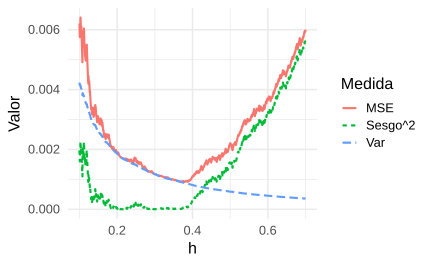
\includegraphics[width=0.7\linewidth]{Notas-Curso-Estadistica_files/figure-latex/MSE-histograma-1} \end{center}

\hypertarget{error-cuadruxe1tico-medio-integrado}{%
\subsection{Error cuadrático medio integrado}\label{error-cuadruxe1tico-medio-integrado}}

El problema con el \(\mathrm{MSE}\left( \hat{f}_h(x)\right)\) es que depende completamente del punto escogido \(x\).

La solución a esto es integrar el MSE.

\begin{align*}
\mathrm{MISE}\left(  \hat{f}_h(x)\right)
& = \mathrm{E}\left[
\int_{ -\infty}^{\infty} \left\{
\hat{f}_h(x) - f(x)
\right\}^2 dx
\right]                                                       \\
& = \int_{ -\infty}^{\infty} \mathrm{E}\left[
\left\{
\hat{f}_h(x) - f(x)
\right\}^2
\right] dx                                                    \\
& = \int_{ -\infty}^{\infty}\mathrm{MSE}(\hat{f}_h(x)) \, dx
\end{align*}

Además,

\begin{align*}
\mathrm{MISE} (\hat{f}_h(x))
& = \int_{ -\infty}^{\infty} \frac{1}{nh} f(x)dx                                                                                                                                          \\
& + \int_{ -\infty}^{\infty}\, \sum_{j}^{} I(x\in B_j) \left\{ \left( j- \frac{1}{2} \right)h -x  \right\}^2 \left [f^\prime \left( \left\{j - \frac{1}{2}\right\}h \right)  \right]^2 dx \\
& = \frac{1}{nh} + \sum_{j}^{} \left [f^\prime \left( \left\{j - \frac{1}{2}\right\}h \right)  \right]^2 \int_{ B_j}    \left\{ \left( j- \frac{1}{2} \right)h -x  \right\}^2 dx          \\
& =\frac{1}{nh} + \frac{h^2}{12} \sum_{j} \left [f^\prime \left( \left\{j - \frac{1}{2}\right\}h \right)  \right]^2                                                                       \\
& \approx \frac{1}{nh} + \frac{h^2}{12} \int \{f^\prime(x)\}^2 dx                                                                                                                         \\
& =\frac{1}{nh} + \frac{h^2}{12} \Vert f^\prime\Vert_{2}^2
\end{align*}

\hypertarget{ancho-de-banda-uxf3ptimo-para-el-histograma}{%
\subsection{Ancho de banda óptimo para el histograma}\label{ancho-de-banda-uxf3ptimo-para-el-histograma}}

El MISE tiene el mismo comportamiento que el MSE. La figura siguiente presenta el comportamiento de la varianza, sesgo y MISE para nuestro ejemplo.

\begin{figure}

{\centering 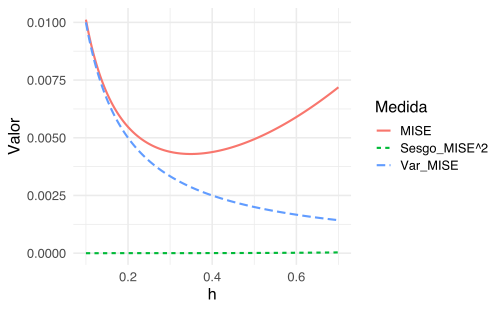
\includegraphics[width=0.7\linewidth]{Notas-Curso-Estadistica_files/figure-latex/MISE-histograma-1} 

}

\caption{ }\label{fig:MISE-histograma}
\end{figure}

La mala elección del parámetro \(h\) causa que el histograma no capture toda la estructura de los datos.

\begin{center}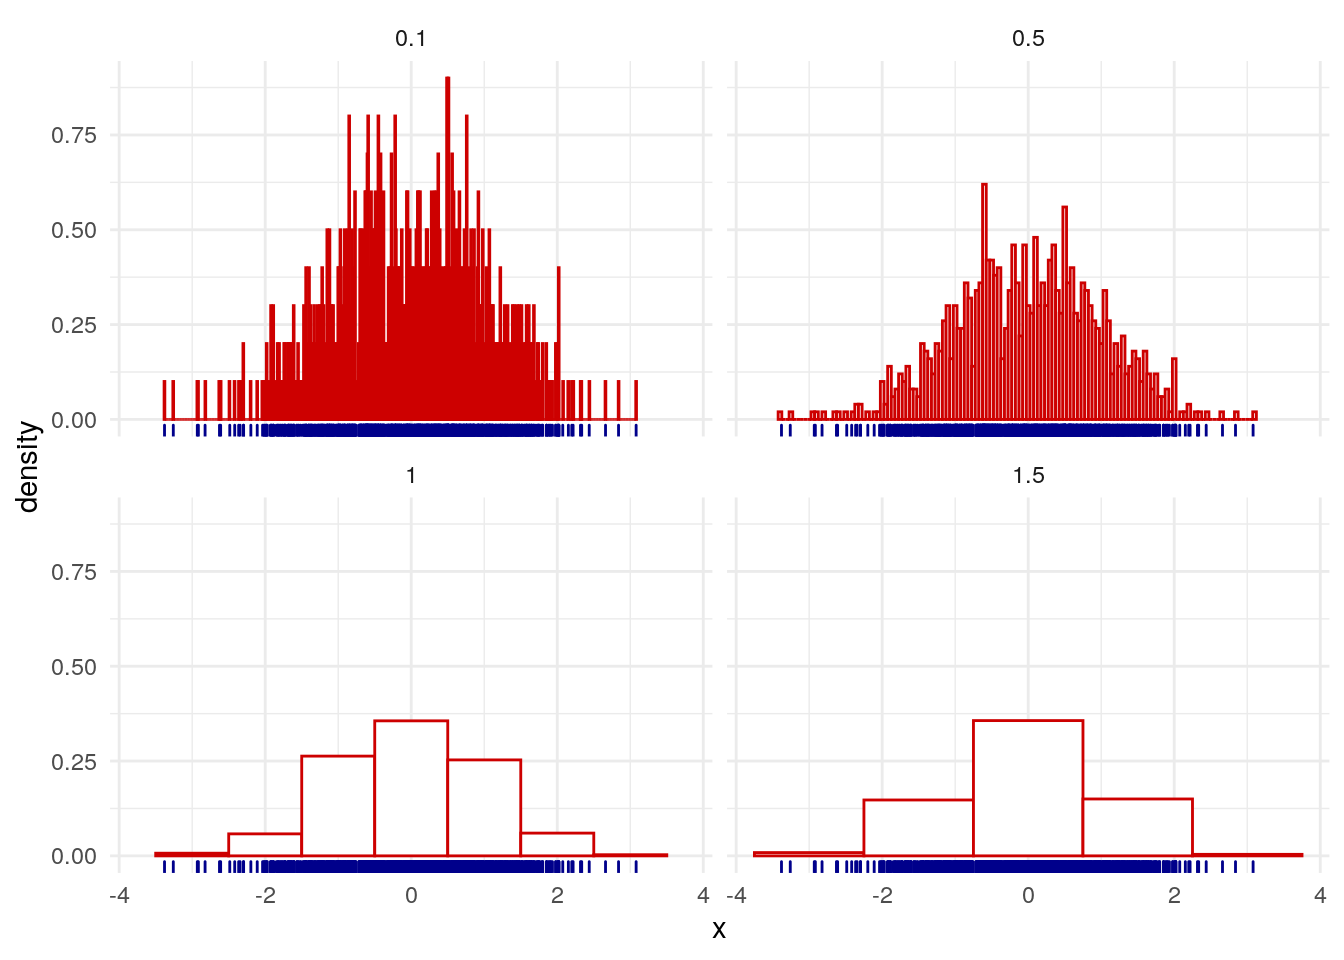
\includegraphics[width=0.7\linewidth]{Notas-Curso-Estadistica_files/figure-latex/unnamed-chunk-8-1} \end{center}

En este caso se puede simplemente minimizar el MISE de la forma usual,

\begin{equation*}
\frac{\partial \mathrm{MISE}(f_{h})}{\partial h} = -\frac{1}{nh^2} + \frac{1}{6} h \Vert f^\prime\Vert_{2}^2 = 0
\end{equation*}

implica que

\begin{equation*}
h_{opt} = \left(\frac{6}{n\Vert f^\prime\Vert_{2}^2}\right) ^{1/3} = O\left( n^{1/3} \right).
\end{equation*}

y que por lo tanto

\begin{equation*}
\mathrm{MISE}(\hat{f}_{h}) = \frac{1}{n} \left(\frac{n\Vert f^\prime\Vert_{2}^2}{6}\right)  ^{1/3}
\end{equation*}

\BeginKnitrBlock{remark}[Recuerde de Estadística I]
\iffalse{} {Nota (Recuerde de Estadística I): } \fi{}Si \(X_1, \ldots, X_2 \sim f_{\theta}\) i.i.d, con \(\mathrm{Var}(X) = \sigma^2\), recuerde que el estimador \(\hat{\theta}\) de \(\theta\) tiene la característica que

\begin{equation*}
\mathrm{MSE}(\theta) = \mathrm{Var}(\hat{\theta}) +
\mathrm{Sesgo}^2(\hat{\theta}) = \frac{\sigma^2}{n}
\end{equation*}
\EndKnitrBlock{remark}

Según la nota anterior la tasas de convergencia del histograma es más lenta que la de un estimador parámetrico considerando la misma cantidad de datos.

\begin{center}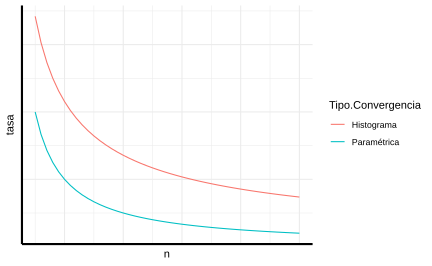
\includegraphics[width=0.7\linewidth]{Notas-Curso-Estadistica_files/figure-latex/unnamed-chunk-10-1} \end{center}

Finalmente, podemos encontrar el valor óptimo de esta datos dado por \(h=\)\texttt{h\_opt\_MISE}

\begin{center}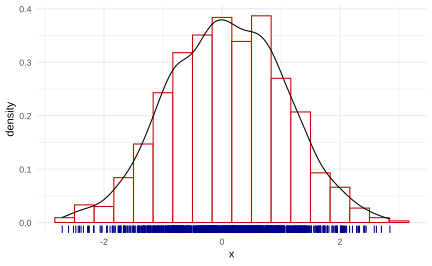
\includegraphics[width=0.7\linewidth]{Notas-Curso-Estadistica_files/figure-latex/unnamed-chunk-12-1} \end{center}

\hypertarget{estimaciuxf3n-no-paramuxe9trica-de-densidad}{%
\section{Estimación No-paramétrica de densidad}\label{estimaciuxf3n-no-paramuxe9trica-de-densidad}}

\hypertarget{primera-construcciuxf3n}{%
\subsection{Primera construcción}\label{primera-construcciuxf3n}}

Sea \(X_{1},\ldots,X_{n}\) variables aleatorias i.i.d. con distribución \(f\) en \(\mathbb{R}\).

La distribución de \(f\) es \(F(x)=\int_{-\infty}^{x}f(t)dt\).

Considere la distribución empírica como
\[
F_{n}(x)=\frac{1}{n}\sum_{i=1}^{n}I(X_{i}\leq x).
\]

Por la ley de los grandes números tenemos que \(\hat{F}_{n}(x) \xrightarrow{c.s} F(x)\) para todo \(x\) en \(\mathbb{R}\)as
\(n\rightarrow\infty\). Entonces, \(F_{n}(x)\) es consistente

para todo \(x\) in \(\mathbb{R}\).

\BeginKnitrBlock{remark}
\iffalse{} {Nota: } \fi{}¿Podríamos derivar \(\hat{F}_n\) para encontrar el estimar \(\hat{f}_n\)?
\EndKnitrBlock{remark}

La respuesta es si (más o menos).

Suponga que \(h>0\) tenemos la aproximación
\[
f(x)\approx\frac{F(x+h)-F(x-h)}{2h}.
\]

Remplazando \(F\) por su estimador \(\hat{F}_{n}\), defina
\[
\hat{f}_{n}^{R}(x)=\frac{F_{n}(x+h)-F_{n}(x-h)}{2h},
\]
donde \(\hat{f}_{n}^{R}(x)\) es el estimador de \emph{Rosenblatt }.

Podemos rescribirlo de la forma,
\[
\hat{f}_{n}^{R}(x)=\frac{1}{2nh}\sum_{i=1}^{n}I(x-h<X_{i}\leq x+h)=\frac{1}{nh}\sum_{i=1}^{n}K_{0}\left(\frac{X_{i}-x}{h}\right)
\]
con \(K_{0}(u)=\frac{1}{2}I(-1<u\leq1)\), lo cuál es equivalente al caso del histograma.

\hypertarget{otra-construcciuxf3n}{%
\subsection{Otra construcción}\label{otra-construcciuxf3n}}

Con el histograma construimos una serie de segmentos fijo \(B_{j}\) y contabamos el número de datos que estaban \textbf{CONTENIDOS en \(B_{j}\)}

\BeginKnitrBlock{remark}
\iffalse{} {Nota: } \fi{}¿Qué pasaría si cambiamos la palabra \textbf{CONTENIDOS} por \textbf{ALREDEDOR DE \enquote{x}}?
\EndKnitrBlock{remark}

Suponga que se tienen intervalos de longitud \$ 2h \$, es decir, intervalos de la forma \$ {[}x-h,x+h) \$.

El histograma se escribe como

\begin{equation*}
\hat{f_{h}}(x) = \dfrac{1}{2hn} \# \{ X_i \in [x-h,x+h) \}.
\end{equation*}

Ahora tratemos de modificar ligeramente esta expresión notando dos cosas

\begin{enumerate}
\def\labelenumi{\arabic{enumi}.}
\item
  \begin{equation*}
  \frac{1}{2} I \left( \left\vert u \right\vert \leq 1 \right)
  \end{equation*}
  con \(u = \frac{x-xi}{h}\)
\item
\end{enumerate}

\begin{equation*}
\frac{1}{2}\# \{ X_i \in [x-h,x+h) \}
=\sum_{i=1}^{n} K\left( \frac{x-x_{i}}{h} \right)
=\sum_{i=1}^{n}  \frac{1}{2} I \left( \left\vert \frac{x-x_{i}}{h}
\right\vert \leq 1 \right)
\end{equation*}
\textbackslash end\{enumerate\}

Finalmente se tiene que

\begin{equation*}
\hat{f}_{h}\left( x \right) = \frac{1}{nh}\sum_{i=1}^{n} K\left( \frac{x-x_{i}}{h} \right)
\end{equation*}

\BeginKnitrBlock{remark}
\iffalse{} {Nota: } \fi{}¿Qué pasaría si cambiaríamos la función \(K\) del histograma por una más general?
\EndKnitrBlock{remark}

Esta función debería cumplir las siguientes características

\begin{itemize}
\tightlist
\item
  \(K(u)\geq 0\).
\item
  \(\int_{-\infty}^{\infty} K(u)du = 1\).
\item
  \(\int_{-\infty}^{\infty} u K(u)du = 0\).
\item
  \(\int_{-\infty}^{\infty} u^{2} K(u)du <\infty\).
\end{itemize}

Por ejemplo:

\begin{itemize}
\tightlist
\item
  \textbf{Uniforme:} \(\frac{1}{2} I \left( \left\vert u \right\vert \leq 1 \right)\).
\item
  \textbf{Triangular:} \((1-|u|) I \left( \left\vert u \right\vert \leq 1 \right)\).
\item
  \textbf{Epanechnikov:} \(\frac{3}{4} (1-u^{2}) I \left( \left\vert u \right\vert \leq 1 \right)\).
\item
  \textbf{Gausian:} \(\frac{1}{\sqrt{2\pi}} \exp \left( -\frac{1}{2}u^{2} \right)\).
\end{itemize}

\begin{center}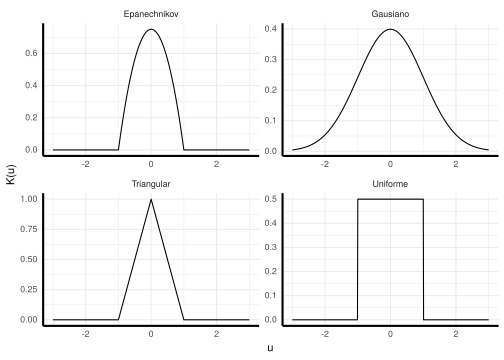
\includegraphics[width=0.7\linewidth]{Notas-Curso-Estadistica_files/figure-latex/unnamed-chunk-16-1} \end{center}

Entonces se tendría que la expresión general para un estimador por núcleos es

\begin{equation*}
\hat{f}_{h}\left( x \right) = \frac{1}{nh}\sum_{i=1}^{n} K\left( \frac{x-x_{i}}{h} \right)
\end{equation*}

\BeginKnitrBlock{remark}
\iffalse{} {Nota: } \fi{}¿Qué pasaría si modificamos el ancho de banda \(h\) para un mismo kernel?
\EndKnitrBlock{remark}

Nuevamente sería el ancho de banda ya que

\begin{center}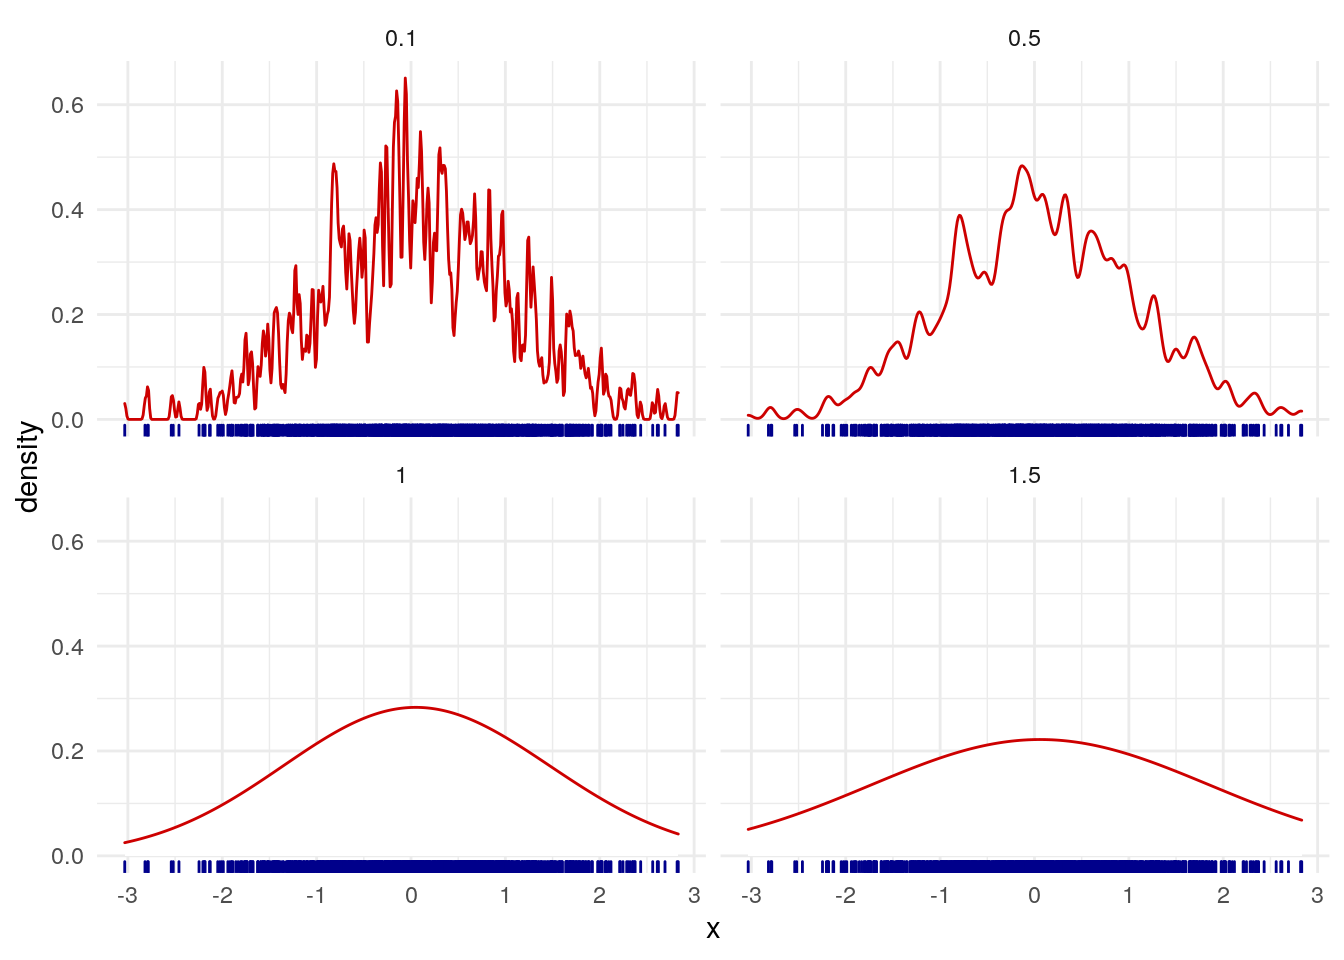
\includegraphics[width=0.7\linewidth]{Notas-Curso-Estadistica_files/figure-latex/unnamed-chunk-18-1} \end{center}

\BeginKnitrBlock{remark}
\iffalse{} {Nota: } \fi{}¿Qué pasaría si modificamos el kernel para un mismo ancho de banda \(h\)?
\EndKnitrBlock{remark}

\begin{center}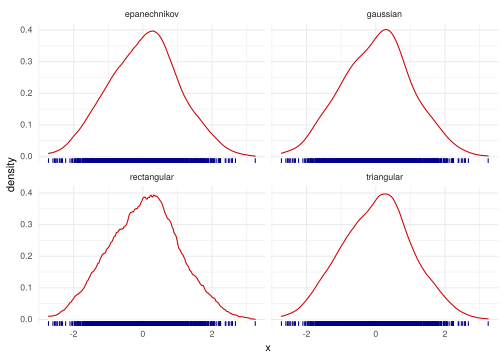
\includegraphics[width=0.7\linewidth]{Notas-Curso-Estadistica_files/figure-latex/unnamed-chunk-20-1} \end{center}

Recordemos nuevamente la fórmula

\begin{equation*}
\hat{f}_{h}\left( x \right) = \frac{1}{nh}\sum_{i=1}^{n} K\left( \frac{x-X_{i}}{h} \right)
\end{equation*}

Cada sumando de esta expresión es una función por si misma. Si la integramos se obtiene que

\begin{equation*}
\frac{1}{nh}\int K\left( \frac{x-X_{i}}{h} \right) dx
= \frac{1}{nh} \int K\left( u \right) h du
= \frac{1}{n} \int K(u) du
= \frac{1}{n}
\end{equation*}

\begin{center}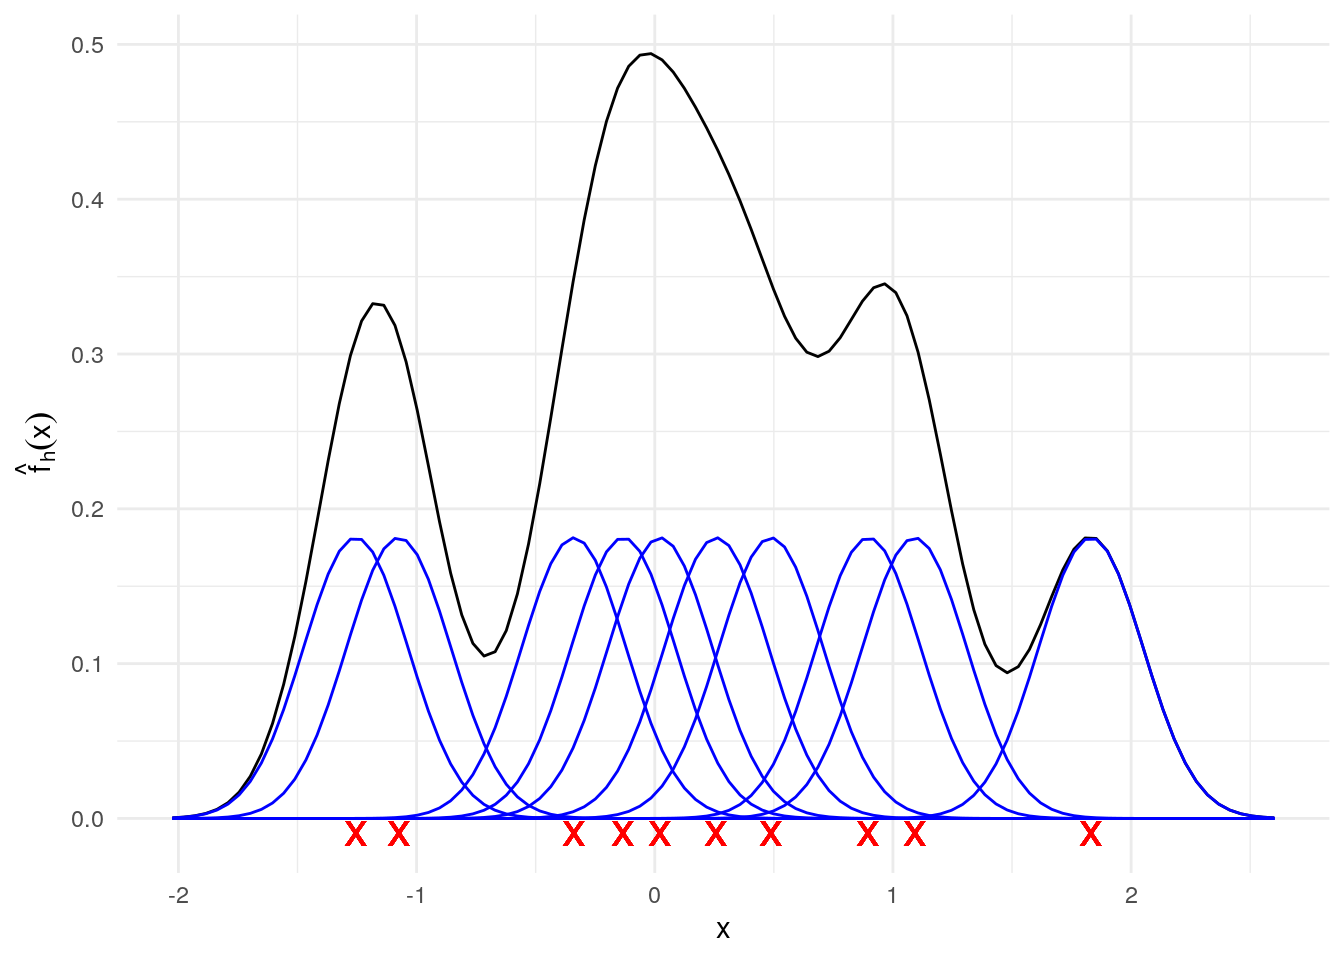
\includegraphics[width=0.7\linewidth]{Notas-Curso-Estadistica_files/figure-latex/unnamed-chunk-21-1} \end{center}

\hypertarget{propiedades-estaduxedsticas-1}{%
\section{Propiedades Estadísticas}\label{propiedades-estaduxedsticas-1}}

\BeginKnitrBlock{remark}
\iffalse{} {Nota: } \fi{}¿Podríamos imitar lo mismo que hicimos para el histograma?
\EndKnitrBlock{remark}

Si. Las propiedades que vimos anteriormente son universales para estimadores.

Entonces:
\begin{align*}
\mathrm{MSE}(\hat{f}_{h}(x)) & =\mathrm{Var}(\hat{f}_{h}(x))+\mathrm{Sesgo}^{2} (\hat{f}_{h}(x))            \\
\mathrm{MISE}(\hat{f}_{h})   & =\int\mathrm{Var}(\hat{f}_{h}(x))dx+\int\mathrm{Sesgo}^{2}(\hat{f}_{h}(x))dx
\end{align*}

donde

\(\mathrm{Var}\left(\hat{f}_{h}(x)\right)=\mathbb{E}\left[\hat{f}_{h}(x)-\mathbb{E}\hat{f}_{h}(x)\right]^{2}\) and \(\mathrm{Sesgo}\left(\hat{f}_{h}(x)\right)=\mathbb{E}\left[\hat{f}_{h}(x)\right]-f(x)\).

\hypertarget{varianza-1}{%
\subsection{Varianza}\label{varianza-1}}

\begin{align*}
\mathrm{Var}(\hat{f}_{h}(x))
& =\mathrm{Var}\left(\frac{1}{n}\sum_{i=1}^{n}K\left(\frac{x-X_{i}}{h}\right)\right)          \\
& =\frac{1}{n^{2}h^{2}}\sum_{i=1}^{n}\mathrm{Var}\left(K\left(\frac{x-X_{i}}{h}\right)\right) \\
& =\frac{1}{nh^{2}}\mathrm{Var}\left(K\left(\frac{x-X}{h}\right)\right)                       \\
& =\frac{1}{nh^{2}}\left\{
\textcolor{red}{\mathbb{E}\left[K^{2}\left(\frac{x-X}{h}\right)\right]}
-\left\{
\textcolor{blue}{\mathbb{E}\left[K\left(\frac{x-X}{h}\right)\right]}
\right\}^{2}
\right\}.
\end{align*}
Usando que:
\begin{align*}
\textcolor{red}{\mathbb{E}\left[K^{2}\left(\frac{x-X}{h}\right)\right]}
& =\int K^{2}\left(\frac{x-s}{h}\right)f(s)ds            \\
& =h\int K^{2}\left(u\right)f(uh+x)du                    \\
& =h\int K^{2}\left(u\right)\left\{ f(x)+o(1)\right\} du \\
& =h\left\{ \Vert K\Vert_{2}^{2}f(x)+o(1)\right\} .
\end{align*}

\begin{align*}
\textcolor{blue}{\mathbb{E}\left[K\left(\frac{x-X}{h}\right)\right]}
& =\int K\left(\frac{x-s}{h}\right)f(s)ds            \\
& = h\int K\left(u\right)f(uh+x)du                    \\
& =h\int K\left(u\right)\left\{ f(x)+o(1)\right\} du \\
& =h\left\{f(x)+o(1)\right\} .
\end{align*}

Por lo tanto se obtiene que

\begin{equation*}
\mathrm{Var}\left(\hat{f}_{h}(x)\right) = \frac{1}{nh} \Vert K\Vert_{2}^{2}f(x) + o\left(\frac{1}{nh}\right), \text{ si } nh\to \infty.
\end{equation*}

\hypertarget{sesgo-1}{%
\subsection{Sesgo}\label{sesgo-1}}

Para el sesgo tenemos

\begin{align*}
\mathrm{Sesgo}\left(\hat{f}_{h}(x)\right)
& = \mathbb{E}\left[\hat{f}_{h}(x)\right]-f(x)                                                  \\
& = \frac{1}{nh} \sum_{i=1}^{n} \mathrm{E}\left[K\left( \frac{x-X_{i}}{h} \right)\right] - f(x) \\
& = \frac{1}{h}\mathrm{E}\left[K\left( \frac{x-X_{1}}{h} \right)\right] - f(x)                  \\
& = \int \frac{1}{h} K\left( \frac{x-u}{h}\right)f(u)du -f(x)                                   \\
\end{align*}

\BeginKnitrBlock{exercise}
\protect\hypertarget{exr:unnamed-chunk-23}{}{\label{exr:unnamed-chunk-23} }Usando el cambio de variable \(s=\frac{u-x}{h}\) y las propiedades del kernel pruebe que

\begin{equation*}
\mathrm{Sesgo}\left(\hat{f}_{h}(x)\right) = \frac{h^{2}}{2} f^{\prime\prime} \mu_{2}(K) + o(h^{2}), \text{ si } h\to 0
\end{equation*}
donde \(\mu_{2}=\int s^{2}K(s)ds\).

\emph{**Nota:** En algunas pruebas más formales, se necesita
además que  $f^{\prime\prime}$ sea absolutamente continua y que
$\int(f^{\prime\prime\prime}(x))dx<\infty$.}
\EndKnitrBlock{exercise}

\BeginKnitrBlock{solution}
\iffalse{} {Solución. } \fi{}\begin{align*}
\mathrm{Sesgo}(\hat{f_{h}}(x)) & = \int \frac{1}{h} K\left( \frac{x-u}{h} \right) f(u)du - f(x)     \\
& = \frac{1}{h} \int hK(s)f(sh+x) ds - f(x) \\
& = \int K(s)\Biggl[ f(x) + f^{\prime}(x)(sh+x-x)  \\
&  \qquad  + \frac{f^{\prime\prime}(x)}{2}(sh+x-x)^2 + o(h^{2}) \Biggr] - f(x) \\
& = \int K(s)f(x)ds + \int hf^{\prime}(x)sK(s) ds  \\
& \qquad  + \int \frac{h^2}{2} f^{\prime\prime}(x)s^2K(s) ds + o(h^2) - f(x) \\
& = f(x) + 0 + \frac{h^2}{2}f^{\prime\prime}(x)\mu_{2}(K) + o(h^2) - f(x)   \\
& = \frac{h^2}{2}f^{\prime\prime}(x)\mu_{2}(K) + o(h^2) \\
\end{align*}
\EndKnitrBlock{solution}

\begin{center}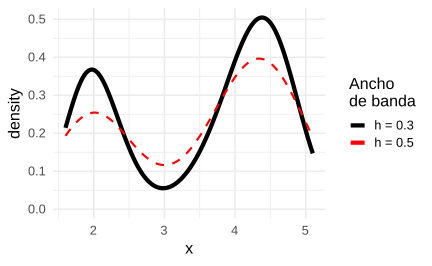
\includegraphics[width=0.7\linewidth]{Notas-Curso-Estadistica_files/figure-latex/unnamed-chunk-25-1} \end{center}

\BeginKnitrBlock{remark}
\iffalse{} {Nota: } \fi{}Note como los cambios en el ancho de banda modifican la suavidad (sesgo) y el aplanamiento de la curva (varianza).
\EndKnitrBlock{remark}

\hypertarget{error-cuadruxe1tico-medio-y-error-cuadruxe1tico-medio-integrado}{%
\subsection{Error cuadrático medio y Error cuadrático medio integrado}\label{error-cuadruxe1tico-medio-y-error-cuadruxe1tico-medio-integrado}}

El error cuadrático medio se escribe
\begin{align*}
\mathrm{MSE}(\hat{f}_{h}(x))
& = \mathrm{Sesgo}\left(\hat{f}_{h}(x)\right)^{2} + \mathrm{Var}\left(\hat{f}_{h}(x)\right)                                                 \\
& = \frac{h^{4}}{4}\left(\mu_{2}(K)f^{\prime\prime}(x)\right)^{2}+\frac{1}{nh}\Vert K\Vert_{2}^{2}f(x)+o(h^{4})+o\left(\frac{1}{nh}\right).
\end{align*}

Y el error cuadrático medio integrado se escribe como,
\begin{align*}
\mathrm{MISE}\left(\hat{f}_{h}\right) & = \int \mathrm{MSE}\left(\hat{f}_{h}(x)\right)dx                                                                                                        \\
& = \int \mathrm{Sesgo}\left(\hat{f}_{h}(x)\right)^{2} + \mathrm{Var}\left(\hat{f}_{h}(x)\right)dx                                                        \\
& = \frac{h^{4}}{4}\mu_{2}^{2}(K)\left\Vert f^{\prime\prime}(x)\right\Vert_{2}^{2} +\frac{1}{nh}\Vert K\Vert_{2}^{2}+o(h^{4})+o\left(\frac{1}{nh}\right).
\end{align*}

\hypertarget{ancho-de-banda-uxf3ptimo}{%
\subsection{Ancho de banda óptimo}\label{ancho-de-banda-uxf3ptimo}}

Minimizando el \(\mathrm{MISE}\) con respecto a \(h\) obtenemos
\begin{equation*}
h_{opt}=\left(\frac{\Vert K\Vert_{2}^{2}}{\Vert f^{\prime\prime}\Vert_{2}^{2}\left(\mu_{2}(K)\right)^{2}n}\right)^{1/5}=O\left( n^{-1/5} \right).
\end{equation*}

\BeginKnitrBlock{remark}
\iffalse{} {Nota: } \fi{}De forma práctica, \(h_{opt}\) no es un estimador útil de \(h\) porque depende de \(\Vert f^{\prime\prime}\Vert_{2}^{2}\) que es desconocido.

Más adelante veremos otra forma de encontrar este estimador.
\EndKnitrBlock{remark}

Evaluando \(h_{opt}\) en el \(\mathrm{MISE}\) tenemos que

\begin{equation*}
\mathrm{MISE}(\hat{f}_{h})=\frac{5}{4}\left(\Vert K\Vert_{2}^{2}\right)^{4/5}\left(\Vert f^{\prime\prime}\Vert_{2}^{2}\mu_{2}(K)\right)^{2/5}n^{-4/5} = O\left( n^{-4/5} \right).
\end{equation*}

\begin{center}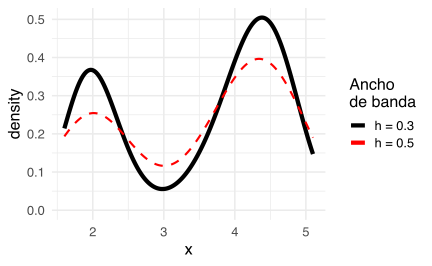
\includegraphics[width=0.7\linewidth]{Notas-Curso-Estadistica_files/figure-latex/unnamed-chunk-28-1} \end{center}

\BeginKnitrBlock{remark}
\iffalse{} {Nota: } \fi{}Formalmente, es posible probar que si \(f\) es \(\beta\) veces continuamente diferenciable y \(\int\left(f^{(\beta)}\right)^{2}<\infty\), entonces se tiene que
\[
{\displaystyle h_{opt}=O\left(n^{-\frac{1}{2\beta+1}}\right).}
\]
Por lo tanto se podría aproximar a una tasa paramétrica de convergencia si
\(\beta\) es grande.
\EndKnitrBlock{remark}

\hypertarget{escogiendo-el-ancho-de-banda}{%
\section{Escogiendo el ancho de banda}\label{escogiendo-el-ancho-de-banda}}

\BeginKnitrBlock{remark}
\iffalse{} {Nota: } \fi{}La principal característica del ancho de banda
\begin{equation*}
h_{opt}=\left(\frac{\Vert K\Vert_{2}^{2}}{\Vert f^{\prime\prime}\Vert_{2}^{2}\left(\mu_{2}(K)\right)^{2}n}\right)^{1/5}=O\left( n^{-1/5} \right).
\end{equation*}

ES QUE ¡NO FUNCIONA!
\EndKnitrBlock{remark}

Veremos dos métodos para determinar un \(h\) que funcione:

\begin{itemize}
\tightlist
\item
  Referencia normal.
\item
  Validación cruzada.
\end{itemize}

\hypertarget{referencia-normal}{%
\subsection{Referencia normal}\label{referencia-normal}}

\BeginKnitrBlock{remark}
\iffalse{} {Nota: } \fi{}Este método es más efectivo si se conoce que la verdadera distribución es bastante suave, unimodal y simétrica.

Más adelante veremos otro método para densidades más generales.
\EndKnitrBlock{remark}

Asuma que \(f\) es normal distribuida y se utiliza un kernel \(K\) gausiano. Entonces se tiene que

\begin{align*}
\hat{h}_{rn} & =\left(\frac{\Vert K\Vert_{2}^{2}}{\Vert f^{\prime\prime}\Vert_{2}^{2}\left(\mu_{2}(K)\right)^{2}n}\right)^{1/5}=O\left( n^{-1/5} \right) \\
& =1.06 \hat{\sigma} n^{-1/5}.
\end{align*}

donde

\begin{equation*}
\hat{\sigma} = \sqrt{\frac{1}{n-1} \sum_{i=1}^{n} \left( x_{i}-\bar{x}^{2} \right)}
\end{equation*}

\BeginKnitrBlock{exercise}
\protect\hypertarget{exr:unnamed-chunk-32}{}{\label{exr:unnamed-chunk-32} }Pruebe que la ecuación anterior es verdadera. Es decir, calcule \(\Vert K\Vert_{2}^{2}\), \(\Vert f^{\prime\prime}\Vert_{2}^{2}\) y \(\mu_{2}(K)\)
\EndKnitrBlock{exercise}

\BeginKnitrBlock{remark}
\iffalse{} {Nota: } \fi{}Un problema con \(\hat{h}_{rn}=1.06 \hat{\sigma} n^{-1/5}\) es su sensibilidad a los valores extremos.
\EndKnitrBlock{remark}

\BeginKnitrBlock{example}
\protect\hypertarget{exm:unnamed-chunk-34}{}{\label{exm:unnamed-chunk-34} }La varianza empírica de 1, 2, 3, 4, 5, es 2.5.

La varianza empírica de 1, 2, 3, 4, 5, 99, es 1538.
\EndKnitrBlock{example}

El rango intercuantil IQR se define como
\begin{equation*}
\mathrm{IQR}^{X} = Q^{X}_{3} - Q^{X}_{1}
\end{equation*}
donde \(Q^{X}_{1}\) y \(Q^{X}_{3}\) son el primer y tercer de un conjunto de datos \(X_{1},\ldots, X_n\).

Con el supuesto que \(X\sim \mathcal{N}(\mu,\sigma^{2})\) entonces \(\displaystyle Z = \frac{X-\mu}{\sigma} \sim \mathcal{N}(0,1)\).

Entonces,
\begin{align*}
\mathrm{IQR}
& = Q^{X}_{3} - Q^{X}_{1}                                                     \\
& = \left( \mu+\sigma Q^{Z}_{3} \right) - \left( \mu+\sigma Q^{Z}_{1} \right) \\
& = \sigma \left(Q^{Z}_{3} - Q^{Z}_{1} \right)                                \\
& \approx \sigma \left( 0.67 - (0.67) \right)                                 \\
& =1.34 \sigma.
\end{align*}

Por lo tanto \(\displaystyle \hat{\sigma} = \frac{\widehat{\mathrm{IQR}}^{X}}{1.34}\)

Podemos sustituir la varianza empírica de la fórmula inicial y tenemos
\begin{equation*}
\hat{h}_{rn} = 1.06 \frac{\widehat{\mathrm{IQR}}^{X}}{1.34} n^{-\frac{1}{5}} \approx 0.79\  \widehat{\mathrm{IQR}}^{X}\ n^{-\frac{1}{5}}
\end{equation*}

Combinando ambos estimadores, podemos obtener,

\begin{equation*}
\hat{h}_{rn} = 1.06 \min \left\{\frac{\widehat{\mathrm{IQR}}^{X}}{1.34}, \hat{\sigma }\right\} n^{-\frac{1}{5}}
\end{equation*}

\hypertarget{validaciuxf3n-cruzada}{%
\subsection{Validación Cruzada}\label{validaciuxf3n-cruzada}}

Defina el \emph{error cuadrático integrado} como
\begin{align*}
\mathrm{ISE}(\hat{f}_{h}) & =\int\left(\hat{f}_{h}(x)-f(x)\right)^{2}dx\nonumber                   \\
& =\int \hat{f}_{h}^{2}(x)dx-2\int \hat{f}_{h}(x)f(x)dx+\int f^{2}(x)dx.
\end{align*}

\BeginKnitrBlock{remark}
\iffalse{} {Nota: } \fi{}El MISE es el valor esperado del ISE.
\EndKnitrBlock{remark}

Nuestro objetivo es minimizar el ISE con respecto a \(h\).

Primero note que \(\int f^{2}(x)dx\) NO DEPENDE de \(h\). Podemos minimizar la expresión
\begin{equation*}
\mathrm{ISE}(\hat{f}_{h})-\int f^{2}(x)dx=
\textcolor{red}{\int\hat{f}_{h}^{2}(x)dx}
-2
\textcolor{blue}{\int\hat{f}_{h}(x)f(x)dx}
\end{equation*}

Vamos a resolver esto en dos pasos partes

\textbf{Integral \(\textcolor{blue}{\int\hat{f}_{h}(x)f(x)dx}\)}

El término \(\textcolor{blue}{\int\hat{f}_{h}(x)f(x)dx}\) es el valor esperado de
\(\mathrm{E}\left[\hat{f}(X)\right]\). Su estimador es
\begin{equation*}
\widehat{\mathrm{E}\left[\hat{f}(X)\right]}
= \frac{1}{n}\sum_{i=1}^{n}\hat{f}_{h}(X_{i})
=\frac{1}{n^{2}h}\sum_{i=1}^{n}\sum_{j=1}^{n}
K\left(\frac{X_{j}-X_{i}}{h}\right).
\end{equation*}

\BeginKnitrBlock{remark}
\iffalse{} {Nota: } \fi{}El problema con esta expresión es que las observaciones que se usan para estimar la esperanza son las misma que se usan para estimar \(\hat{f}_{h}(x)\) (Se utilizan doble).
\EndKnitrBlock{remark}

La solución es remover la \(i^{\text{ésima}}\) observación de \(\hat{f}_{h}\) para cada \(i\).

Redefiniendo el estimador anterior tenemos \(\int \hat{f}_{h}(x)f(x)dx\) como
\[
\frac{1}{n}\sum_{i=1}^{n}\hat{f}_{h,-i}(X_{i}),
\]
donde
\[
\hat{f}_{h,-i}(x)=\frac{1}{(n-1)h}\sum_{\substack{j=1\\ j\neq i}}^{n}K\left( \frac{x-X_{i}}{h} \right) .
\]

\textbf{Integral \(\textcolor{red}{\int\hat{f}_{h}^{2}(x)dx}\)}

Siguiendo con el término \(\textcolor{red}{\int\hat{f}_{h}^{2}(x)dx}\) note que este se puede reescribir como

\begin{align*}
\textcolor{red}{\int\hat{f}_{h}^{2}(x)dx}
& =\int\left(\frac{1}{nh}\sum_{i=1}^{n}K\left( \frac{x-X_{i}}{h} \right)\right)^{2}dx                                    \\
& =\frac{1}{n^{2}h^{2}}\sum_{i=1}^{n}\sum_{i=1}^{n}\int K\left(\frac{x-X_{i}}{h}\right)K\left(\frac{x-X_{j}}{h}\right)dx \\
& =\frac{1}{n^{2}h}\sum_{i=1}^{n}\sum_{i=1}^{n}\int K\left(u\right)K\left(\frac{X_{i}-X_{j}}{h}-u\right)du               \\
& =\frac{1}{n^{2}h}\sum_{i=1}^{n}\sum_{i=1}^{n}K*K\left(\frac{X_{i}-X_{j}}{h}\right).
\end{align*}

donde \(K*K\) es la convolución de \(K\) consigo misma.

Finalmente tenemos la función,

\[
\mathrm{CV}(h)=\frac{1}{n^{2}h}\sum_{i=1}^{n}\sum_{j=1}^{n}K*K\left(\frac{X_{i}-X_{j}}{h}\right)-\frac{2}{(n-1)h}\sum_{i=1}^{n}\mathop{\sum_{j=1}^{n}}_{j\neq i}K\left( \frac{X_{i}-X_{j}}{h} \right).
\]

\BeginKnitrBlock{remark}
\iffalse{} {Nota: } \fi{}Note que \(\mathrm{CV}(h)\) no depende de \(f\) o sus derivadas.
\EndKnitrBlock{remark}

\BeginKnitrBlock{remark}
\iffalse{} {Nota: } \fi{}Para efectos prácticos es mejor utilizar el criterio

\[
CV(h)=\int\hat{f}_{h}^{2}(x)dx-\frac{2}{(n-1)h}\sum_{i=1}^{n}\mathop{\sum_{j=1}^{n}}_{j\neq i}K\left( \frac{X_{i}-X_{j}}{h} \right)
\]
y luego calcular numéricamente la integral.
\EndKnitrBlock{remark}

\hypertarget{intervalos-de-confianza-para-estimadores-de-densidad-no-paramuxe9tricos}{%
\subsection{Intervalos de confianza para estimadores de densidad no paramétricos}\label{intervalos-de-confianza-para-estimadores-de-densidad-no-paramuxe9tricos}}

Usando los resultados anteriores y asumiendo que \(h=cn^{-\frac{1}{5}}\) entonces

\begin{equation*}
n^{-\frac{2}{5}} \left\{ \hat{f}_{h}(x) -f(x)\right\}
\xrightarrow{\mathcal{L}} \mathcal{N}\left(\underbrace{\frac{c^{2}}{2} f^{\prime\prime}
\mu_{2}(K)}_{b_{x}}, \underbrace{\frac{1}{c}f(x) \left\Vert K \right\Vert_{2}^{2}}_{v_{x}}\right).
\end{equation*}

Si \(z_{1-\frac{\alpha}{2}}\) es el cuantil \(1-\frac{\alpha}{2}\) de una distribución normal estándar, entonces

\begin{align*}
1-\alpha
& \approx \mathbb{P}\left(b_{x}-z_{1-\frac{\alpha}{2}} v_{x} \leq n^{2 / 5}\left\{\widehat{f}_{h}(x)-f(x)\right\} \leq b_{x}+z_{1-\frac{\alpha}{2}} v_{x}\right) \\
& =\mathbb{P}\left(\widehat{f}_{h}(x)-n^{-2 / 5}\left\{b_{x}+z_{1-\frac{\alpha}{2}} v_{x}\right\}\right.                                                         \\
& \qquad\qquad \left. \leq f(x)\leq \hat{f}_{h}(x)-n^{-2 / 5}\left\{b_{x}-z_{1-\frac{\alpha}{2}} v_{x}\right\}\right)
\end{align*}

Esta expresión nos dice que con una probabilidad de \(1-\alpha\) se tiene que

\begin{equation*}
\begin{aligned}
& \left[\hat{f}_{h}(x)-\frac{h^{2}}{2} f^{\prime \prime}(x) \mu_{2}(K)-z_{1-\frac{\alpha}{2}} \sqrt{\frac{f(x)\|K\|_{2}^{2}}{n h}}\right. \\
& \left.\widehat{f}_{h}(x)-\frac{h^{2}}{2} f^{\prime \prime}(x) \mu_{2}(K)+z_{1-\frac{a}{2}} \sqrt{\frac{f(x)\|K\|_{2}^{2}}{n h}}\right]
\end{aligned}
\end{equation*}

Al igual que en los casos anteriores, este invtervalo no es útil ya que depende de \(f(x)\) y \(f^{\prime\prime} (x)\).

Si \(h\) es pequeño relativamente a \(n^{-\frac{1}{5}}\) entonces el segundo término \(\frac{h^{2}}{2} f^{\prime \prime}(x) \mu_{2}(K)\) podría ser ignorado.

Podemos reemplazar \(f(x)\) por su estimador \(\hat{f}_{h}(x)\). Entonces tendríamos una intervalo aplicable a nuestro caso

\begin{equation*}
\left[\hat{f_{h}}(x)-z_{1-\frac{\alpha}{2}} \sqrt{\frac{\hat{f_{h}}(x)\|K\|_{2}^{2}}{n h}}, \hat{f}_{h}(x)+z_{1-\frac{\alpha}{2}} \sqrt{\frac{\hat{f}_{h}(x)\|\mathrm{K}\|_{2}^{2}}{n h}}\right]
\end{equation*}

\BeginKnitrBlock{remark}
\iffalse{} {Nota: } \fi{}Este intervalo de confianza solo funciona en cada punto particular de \(f(x)\).

Existe una versión más general para determinar la banda de confianza de toda la función. Por favor revisar la página 62 de \autocite{Hardle2004}.
\EndKnitrBlock{remark}

\hypertarget{laboratorio}{%
\section{Laboratorio}\label{laboratorio}}

Comenzaremos con una librería bastante básica llamada \texttt{KernSmooth}.

\hypertarget{efecto-de-distintos-kernels-en-la-estimaciuxf3n}{%
\subsection{Efecto de distintos Kernels en la estimación}\label{efecto-de-distintos-kernels-en-la-estimaciuxf3n}}

\begin{Shaded}
\begin{Highlighting}[]
\NormalTok{x <-}\StringTok{ }\KeywordTok{read.csv}\NormalTok{(}\StringTok{"data/stockres.txt"}\NormalTok{)}
\NormalTok{x <-}\StringTok{ }\KeywordTok{unlist}\NormalTok{(x)}
\end{Highlighting}
\end{Shaded}

\begin{Shaded}
\begin{Highlighting}[]
\KeywordTok{summary}\NormalTok{(x)}
\end{Highlighting}
\end{Shaded}

\begin{verbatim}
##       Min.    1st Qu.     Median       Mean    3rd Qu.       Max. 
## -0.6118200 -0.0204085 -0.0010632 -0.0004988  0.0215999  0.1432286
\end{verbatim}

\begin{Shaded}
\begin{Highlighting}[]
\KeywordTok{library}\NormalTok{(KernSmooth)}

\NormalTok{fhat_normal <-}\StringTok{ }\KeywordTok{bkde}\NormalTok{(x, }\DataTypeTok{kernel =} \StringTok{"normal"}\NormalTok{, }\DataTypeTok{bandwidth =} \FloatTok{0.05}\NormalTok{)}
\KeywordTok{plot}\NormalTok{(fhat_normal, }\DataTypeTok{type =} \StringTok{"l"}\NormalTok{)}
\end{Highlighting}
\end{Shaded}

\begin{center}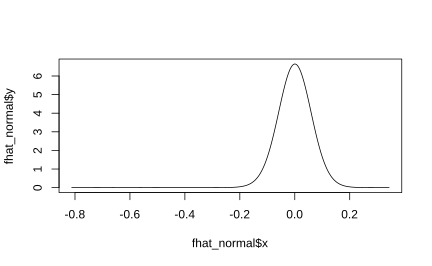
\includegraphics[width=0.7\linewidth]{Notas-Curso-Estadistica_files/figure-latex/unnamed-chunk-42-1} \end{center}

\begin{Shaded}
\begin{Highlighting}[]
\NormalTok{fhat_unif <-}\StringTok{ }\KeywordTok{bkde}\NormalTok{(x, }\DataTypeTok{kernel =} \StringTok{"box"}\NormalTok{, }\DataTypeTok{bandwidth =} \FloatTok{0.05}\NormalTok{)}
\KeywordTok{plot}\NormalTok{(fhat_unif, }\DataTypeTok{type =} \StringTok{"l"}\NormalTok{)}
\end{Highlighting}
\end{Shaded}

\begin{center}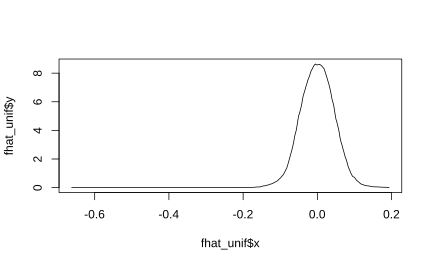
\includegraphics[width=0.7\linewidth]{Notas-Curso-Estadistica_files/figure-latex/unnamed-chunk-42-2} \end{center}

\begin{Shaded}
\begin{Highlighting}[]
\NormalTok{fhat_epanech <-}\StringTok{ }\KeywordTok{bkde}\NormalTok{(x, }\DataTypeTok{kernel =} \StringTok{"epanech"}\NormalTok{, }\DataTypeTok{bandwidth =} \FloatTok{0.05}\NormalTok{)}
\KeywordTok{plot}\NormalTok{(fhat_epanech, }\DataTypeTok{type =} \StringTok{"l"}\NormalTok{)}
\end{Highlighting}
\end{Shaded}

\begin{center}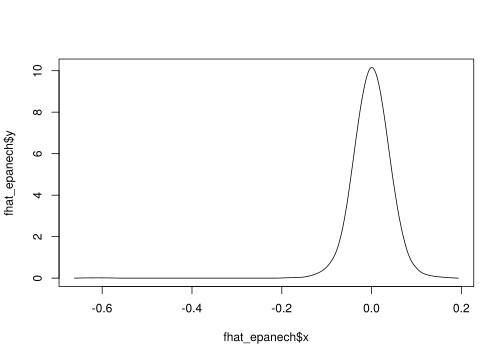
\includegraphics[width=0.7\linewidth]{Notas-Curso-Estadistica_files/figure-latex/unnamed-chunk-42-3} \end{center}

\begin{Shaded}
\begin{Highlighting}[]
\NormalTok{fhat_biweight <-}\StringTok{ }\KeywordTok{bkde}\NormalTok{(x, }\DataTypeTok{kernel =} \StringTok{"biweight"}\NormalTok{, }\DataTypeTok{bandwidth =} \FloatTok{0.05}\NormalTok{)}
\KeywordTok{plot}\NormalTok{(fhat_biweight, }\DataTypeTok{type =} \StringTok{"l"}\NormalTok{)}
\end{Highlighting}
\end{Shaded}

\begin{center}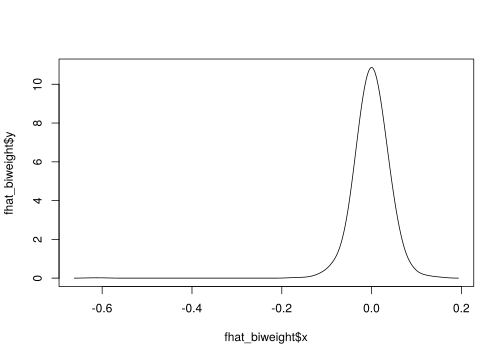
\includegraphics[width=0.7\linewidth]{Notas-Curso-Estadistica_files/figure-latex/unnamed-chunk-42-4} \end{center}

\begin{Shaded}
\begin{Highlighting}[]
\NormalTok{fhat_triweight <-}\StringTok{ }\KeywordTok{bkde}\NormalTok{(x, }\DataTypeTok{kernel =} \StringTok{"triweight"}\NormalTok{, }\DataTypeTok{bandwidth =} \FloatTok{0.05}\NormalTok{)}
\KeywordTok{plot}\NormalTok{(fhat_triweight, }\DataTypeTok{type =} \StringTok{"l"}\NormalTok{)}
\end{Highlighting}
\end{Shaded}

\begin{center}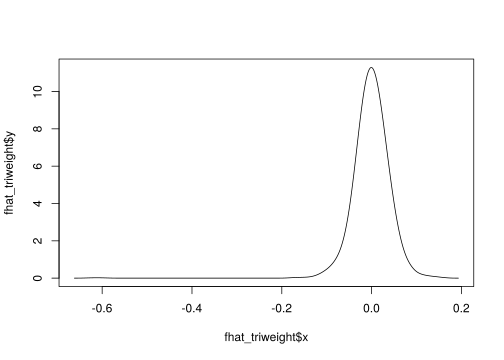
\includegraphics[width=0.7\linewidth]{Notas-Curso-Estadistica_files/figure-latex/unnamed-chunk-42-5} \end{center}

\hypertarget{efecto-del-ancho-de-banda-en-la-estimaciuxf3n}{%
\subsection{Efecto del ancho de banda en la estimación}\label{efecto-del-ancho-de-banda-en-la-estimaciuxf3n}}

** Kernel uniforme **

\begin{Shaded}
\begin{Highlighting}[]
\NormalTok{fhat <-}\StringTok{ }\KeywordTok{bkde}\NormalTok{(x, }\DataTypeTok{kernel =} \StringTok{"box"}\NormalTok{, }\DataTypeTok{bandwidth =} \FloatTok{0.001}\NormalTok{)}
\KeywordTok{plot}\NormalTok{(fhat, }\DataTypeTok{type =} \StringTok{"l"}\NormalTok{)}
\end{Highlighting}
\end{Shaded}

\begin{center}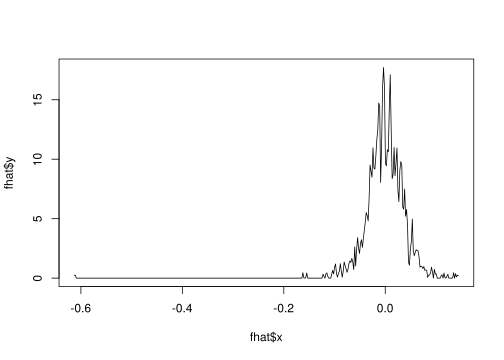
\includegraphics[width=0.7\linewidth]{Notas-Curso-Estadistica_files/figure-latex/unnamed-chunk-43-1} \end{center}

\begin{Shaded}
\begin{Highlighting}[]
\NormalTok{fhat <-}\StringTok{ }\KeywordTok{bkde}\NormalTok{(x, }\DataTypeTok{kernel =} \StringTok{"box"}\NormalTok{, }\DataTypeTok{bandwidth =} \FloatTok{0.5}\NormalTok{)}
\KeywordTok{plot}\NormalTok{(fhat, }\DataTypeTok{type =} \StringTok{"l"}\NormalTok{)}
\end{Highlighting}
\end{Shaded}

\begin{center}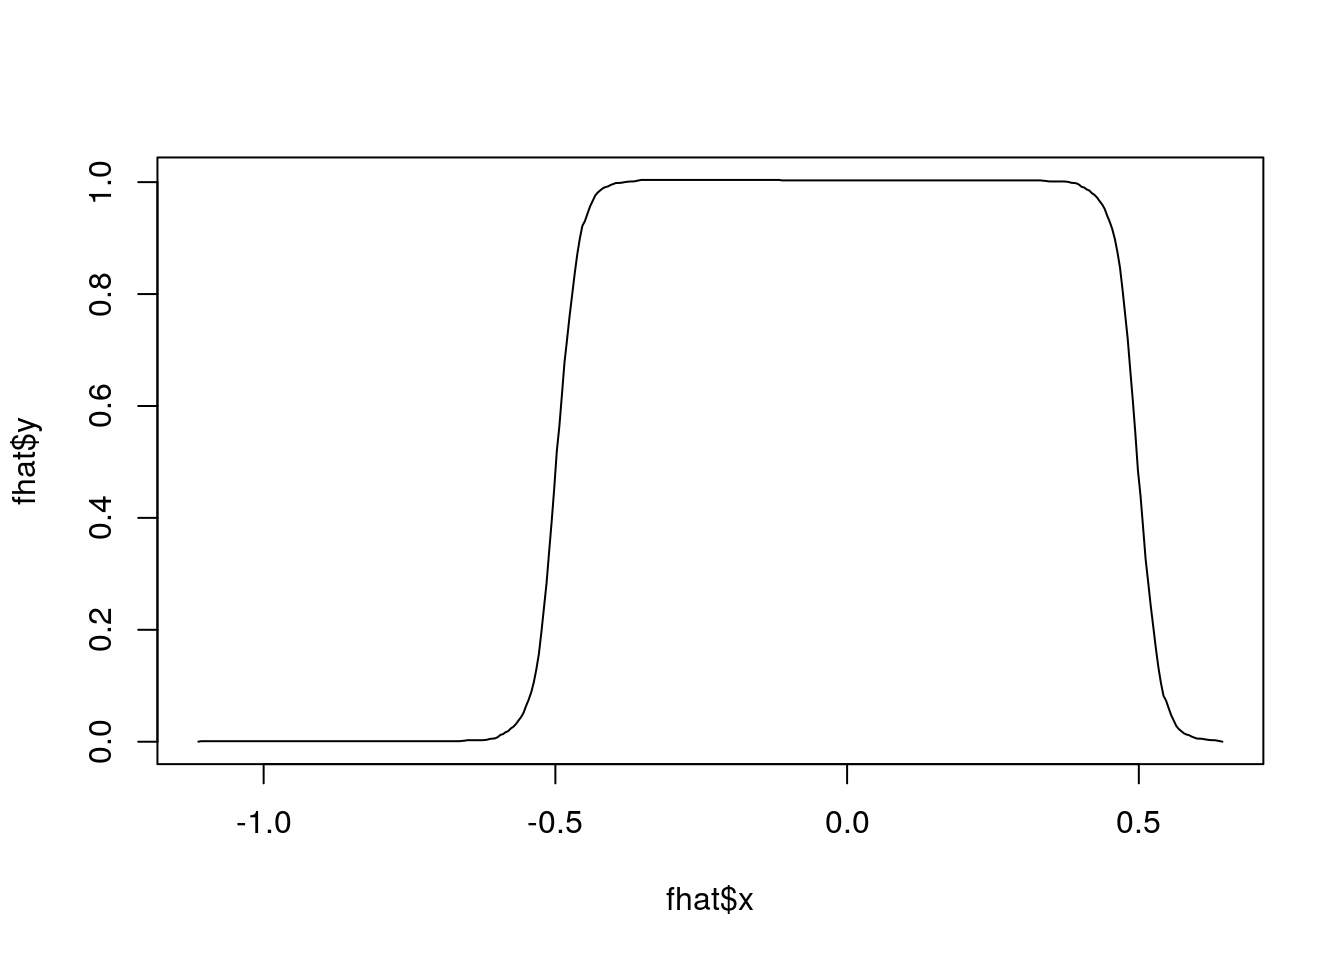
\includegraphics[width=0.7\linewidth]{Notas-Curso-Estadistica_files/figure-latex/unnamed-chunk-43-2} \end{center}

** Kernel Epanechnikov **

\begin{Shaded}
\begin{Highlighting}[]
\NormalTok{fhat <-}\StringTok{ }\KeywordTok{bkde}\NormalTok{(x, }\DataTypeTok{kernel =} \StringTok{"epa"}\NormalTok{, }\DataTypeTok{bandwidth =} \FloatTok{0.001}\NormalTok{)}
\KeywordTok{plot}\NormalTok{(fhat, }\DataTypeTok{type =} \StringTok{"l"}\NormalTok{)}
\end{Highlighting}
\end{Shaded}

\begin{center}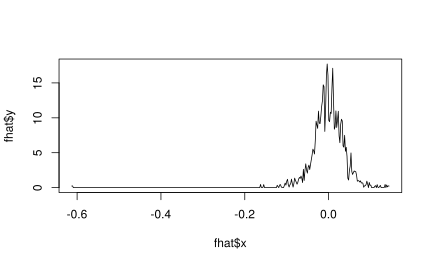
\includegraphics[width=0.7\linewidth]{Notas-Curso-Estadistica_files/figure-latex/unnamed-chunk-44-1} \end{center}

\begin{Shaded}
\begin{Highlighting}[]
\NormalTok{fhat <-}\StringTok{ }\KeywordTok{bkde}\NormalTok{(x, }\DataTypeTok{kernel =} \StringTok{"epa"}\NormalTok{, }\DataTypeTok{bandwidth =} \FloatTok{0.5}\NormalTok{)}
\KeywordTok{plot}\NormalTok{(fhat, }\DataTypeTok{type =} \StringTok{"l"}\NormalTok{)}
\end{Highlighting}
\end{Shaded}

\begin{center}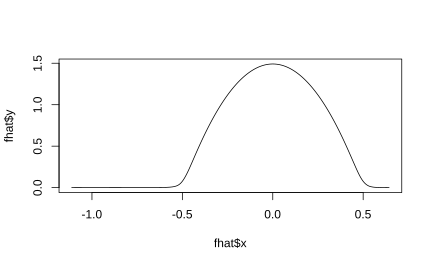
\includegraphics[width=0.7\linewidth]{Notas-Curso-Estadistica_files/figure-latex/unnamed-chunk-44-2} \end{center}

\begin{Shaded}
\begin{Highlighting}[]
\KeywordTok{suppressMessages}\NormalTok{(}\KeywordTok{library}\NormalTok{(tidyverse))}
\KeywordTok{library}\NormalTok{(gganimate)}

\NormalTok{fani <-}\StringTok{ }\KeywordTok{tibble}\NormalTok{()}

\ControlFlowTok{for}\NormalTok{ (b }\ControlFlowTok{in} \KeywordTok{seq}\NormalTok{(}\FloatTok{0.001}\NormalTok{, }\FloatTok{0.02}\NormalTok{, }\DataTypeTok{length.out =} \DecValTok{40}\NormalTok{)) \{}
\NormalTok{    f <-}\StringTok{ }\KeywordTok{bkde}\NormalTok{(x, }\DataTypeTok{kernel =} \StringTok{"epa"}\NormalTok{, }\DataTypeTok{bandwidth =}\NormalTok{ b, }\DataTypeTok{gridsize =} \KeywordTok{length}\NormalTok{(x))}
\NormalTok{    fani <-}\StringTok{ }\NormalTok{fani }\OperatorTok\StringTok{ }\KeywordTok{bind_rows}\NormalTok{(}\KeywordTok{tibble}\NormalTok{(}\DataTypeTok{xreal =} \KeywordTok{sort}\NormalTok{(x), }
        \DataTypeTok{x =}\NormalTok{ f}\OperatorTok{$}\NormalTok{x, }\DataTypeTok{y =}\NormalTok{ f}\OperatorTok{$}\NormalTok{y, }\DataTypeTok{bw =}\NormalTok{ b))}
\NormalTok{\}}

\KeywordTok{ggplot}\NormalTok{(}\DataTypeTok{data =}\NormalTok{ fani) }\OperatorTok{+}\StringTok{ }\KeywordTok{geom_line}\NormalTok{(}\KeywordTok{aes}\NormalTok{(x, y), }\DataTypeTok{color =} \StringTok{"blue"}\NormalTok{) }\OperatorTok{+}\StringTok{ }
\StringTok{    }\KeywordTok{labs}\NormalTok{(}\DataTypeTok{title =} \KeywordTok{paste0}\NormalTok{(}\StringTok{"Ancho de banda = \{closest_state\}"}\NormalTok{)) }\OperatorTok{+}\StringTok{ }
\StringTok{    }\KeywordTok{transition_states}\NormalTok{(bw) }\OperatorTok{+}\StringTok{ }\KeywordTok{view_follow}\NormalTok{() }\OperatorTok{+}\StringTok{ }\KeywordTok{theme_minimal}\NormalTok{(}\DataTypeTok{base_size =} \DecValTok{20}\NormalTok{)}

\CommentTok{# anim_save('manual_figure/bandwidth-animation.gif')}
\end{Highlighting}
\end{Shaded}

\BeginKnitrBlock{remark}
\iffalse{} {Nota: } \fi{}
- Construya una variable llamada \texttt{u} que sea una secuencia de -0.15 a 0.15 con un paso de 0.01
- Asigne \texttt{x} a los datos \texttt{stockrel} y calcule su media y varianza.
- Usando la función \texttt{dnorm} construya los valores de la distribución de los datos usando la media y varianza calculada anteriormente. Asigne a esta variable \texttt{f\textbackslash{}\_param}.
- Defina un ancho de banda \texttt{h} en 0.02
- Construya un histograma para estos datos con ancho de banda \texttt{h}. Llame a esta variable \texttt{f\textbackslash{}\_hist}
- Usando el paquete \texttt{KernSmooth} y la función \texttt{bkde}, construya una función que calcule el estimador no paramétrico con un núcleo Epanechivok para un ancho de banda \(h\). Llame a esta variable \texttt{f\textbackslash{}\_epa}.
- Dibuje en el mismo gráfico la estimación paramétrica y no paramétrica.
\EndKnitrBlock{remark}

\begin{Shaded}
\begin{Highlighting}[]
\NormalTok{x <-}\StringTok{ }\KeywordTok{read.csv}\NormalTok{(}\StringTok{"data/stockres.txt"}\NormalTok{)}
\NormalTok{x <-}\StringTok{ }\KeywordTok{unlist}\NormalTok{(x)}
\CommentTok{# Eliminar nombres de las columnas}
\KeywordTok{names}\NormalTok{(x) <-}\StringTok{ }\OtherTok{NULL}

\NormalTok{u <-}\StringTok{ }\KeywordTok{seq}\NormalTok{(}\OperatorTok{-}\FloatTok{0.15}\NormalTok{, }\FloatTok{0.15}\NormalTok{, }\DataTypeTok{by =} \FloatTok{0.01}\NormalTok{)}

\NormalTok{mu <-}\StringTok{ }\KeywordTok{mean}\NormalTok{(x)}
\NormalTok{sigma <-}\StringTok{ }\KeywordTok{sd}\NormalTok{(x)}

\NormalTok{f_param <-}\StringTok{ }\KeywordTok{dnorm}\NormalTok{(u, }\DataTypeTok{mean =}\NormalTok{ mu, }\DataTypeTok{sd =}\NormalTok{ sigma)}

\NormalTok{h <-}\StringTok{ }\FloatTok{0.02}

\NormalTok{n_bins <-}\StringTok{ }\KeywordTok{floor}\NormalTok{(}\KeywordTok{diff}\NormalTok{(}\KeywordTok{range}\NormalTok{(x))}\OperatorTok{/}\NormalTok{h)}

\NormalTok{f_hist <-}\StringTok{ }\KeywordTok{hist}\NormalTok{(x, }\DataTypeTok{breaks =}\NormalTok{ n_bins)}
\end{Highlighting}
\end{Shaded}

\begin{center}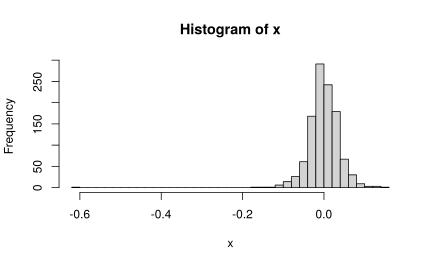
\includegraphics[width=0.7\linewidth]{Notas-Curso-Estadistica_files/figure-latex/unnamed-chunk-47-1} \end{center}

\begin{Shaded}
\begin{Highlighting}[]
\NormalTok{f_epa <-}\StringTok{ }\KeywordTok{as.data.frame}\NormalTok{(}\KeywordTok{bkde}\NormalTok{(x, }\DataTypeTok{kernel =} \StringTok{"epa"}\NormalTok{, }\DataTypeTok{bandwidth =}\NormalTok{ h))}

\NormalTok{x_df <-}\StringTok{ }\KeywordTok{data.frame}\NormalTok{(x)}

\KeywordTok{library}\NormalTok{(ggplot2)}

\KeywordTok{ggplot}\NormalTok{(x_df, }\KeywordTok{aes}\NormalTok{(x)) }\OperatorTok{+}\StringTok{ }\KeywordTok{geom_histogram}\NormalTok{(}\KeywordTok{aes}\NormalTok{(}\DataTypeTok{y =}\NormalTok{ ..density..), }
    \DataTypeTok{binwidth =} \FloatTok{0.02}\NormalTok{, }\DataTypeTok{col =} \StringTok{"black"}\NormalTok{, }\DataTypeTok{fill =} \StringTok{"white"}\NormalTok{) }\OperatorTok{+}\StringTok{ }
\StringTok{    }\KeywordTok{stat_function}\NormalTok{(}\DataTypeTok{fun =}\NormalTok{ dnorm, }\DataTypeTok{args =} \KeywordTok{list}\NormalTok{(}\DataTypeTok{mean =}\NormalTok{ mu, }
        \DataTypeTok{sd =}\NormalTok{ sigma), }\DataTypeTok{color =} \StringTok{"red"}\NormalTok{) }\OperatorTok{+}\StringTok{ }\KeywordTok{geom_line}\NormalTok{(}\DataTypeTok{data =}\NormalTok{ f_epa, }
    \KeywordTok{aes}\NormalTok{(x, y), }\DataTypeTok{color =} \StringTok{"blue"}\NormalTok{) }\OperatorTok{+}\StringTok{ }\KeywordTok{theme_minimal}\NormalTok{(}\DataTypeTok{base_size =} \DecValTok{20}\NormalTok{)}
\end{Highlighting}
\end{Shaded}

\begin{center}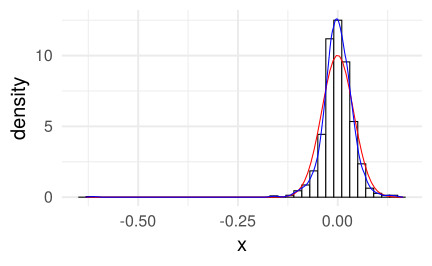
\includegraphics[width=0.7\linewidth]{Notas-Curso-Estadistica_files/figure-latex/unnamed-chunk-47-2} \end{center}

\hypertarget{ancho-de-banda-uxf3ptimo-1}{%
\subsection{Ancho de banda óptimo}\label{ancho-de-banda-uxf3ptimo-1}}

Usemos la regla de la normal o también conocida como Silverman.
\textbf{Primero recuerde que en este caso se asume que \(f(x)\) sigue una distribución normal}. En este caso, lo que se obtiene es que

\begin{align*}
\Vert f^{\prime \prime} \Vert_2^2 & = \sigma ^{-5} \int \{\phi^{\prime \prime}\}^2 dx              \\
& = \sigma ^{-5} \frac{3}{8\sqrt{\pi}} \approx 0.212 \sigma^{-5}
\end{align*}

donde \(\phi\) es la densidad de una normal estándar.

El estimador para \(\sigma\) es

\[
s = \sqrt{\frac{1}{n-1} \sum_{i=1}^n (x_i - \bar{x})^2  }.
\]

Y usando el cálculo realizado anteriormente, se obtiene que

\[
h_{normal} = \left( \frac{4 s^5}{3n} \right)^{1/5} \approx 1.06 s n^{-1/5}.
\]

Un estimador más robusto es

\[
h_{normal} =  1.06 \min \left\{ s , \frac{IQR}{1.34} \right\} n^{-1/5}.
\]

¿Por qué es \(IQR / 1.34\)?

\begin{Shaded}
\begin{Highlighting}[]
\NormalTok{s <-}\StringTok{ }\KeywordTok{sd}\NormalTok{(x)}
\NormalTok{n <-}\StringTok{ }\KeywordTok{length}\NormalTok{(x)}
\end{Highlighting}
\end{Shaded}

\begin{Shaded}
\begin{Highlighting}[]
\NormalTok{h_normal <-}\StringTok{ }\FloatTok{1.06} \OperatorTok{*}\StringTok{ }\NormalTok{s }\OperatorTok{*}\StringTok{ }\NormalTok{n}\OperatorTok{^}\NormalTok{(}\OperatorTok{-}\DecValTok{1}\OperatorTok{/}\DecValTok{5}\NormalTok{)}

\NormalTok{h <-}\StringTok{ }\NormalTok{h_normal}

\NormalTok{n_bins <-}\StringTok{ }\KeywordTok{floor}\NormalTok{(}\KeywordTok{diff}\NormalTok{(}\KeywordTok{range}\NormalTok{(x))}\OperatorTok{/}\NormalTok{h)}
\NormalTok{f_hist <-}\StringTok{ }\KeywordTok{hist}\NormalTok{(x, }\DataTypeTok{breaks =}\NormalTok{ n_bins, }\DataTypeTok{plot =} \OtherTok{FALSE}\NormalTok{)}
\NormalTok{f_epa <-}\StringTok{ }\KeywordTok{as.data.frame}\NormalTok{(}\KeywordTok{bkde}\NormalTok{(x, }\DataTypeTok{kernel =} \StringTok{"epa"}\NormalTok{, }\DataTypeTok{bandwidth =}\NormalTok{ h))}

\KeywordTok{ggplot}\NormalTok{(x_df, }\KeywordTok{aes}\NormalTok{(x)) }\OperatorTok{+}\StringTok{ }\KeywordTok{geom_histogram}\NormalTok{(}\KeywordTok{aes}\NormalTok{(}\DataTypeTok{y =}\NormalTok{ ..density..), }
    \DataTypeTok{binwidth =}\NormalTok{ h, }\DataTypeTok{col =} \StringTok{"black"}\NormalTok{, }\DataTypeTok{fill =} \StringTok{"white"}\NormalTok{) }\OperatorTok{+}\StringTok{ }
\StringTok{    }\KeywordTok{stat_function}\NormalTok{(}\DataTypeTok{fun =}\NormalTok{ dnorm, }\DataTypeTok{args =} \KeywordTok{list}\NormalTok{(}\DataTypeTok{mean =}\NormalTok{ mu, }
        \DataTypeTok{sd =}\NormalTok{ sigma), }\DataTypeTok{color =} \StringTok{"red"}\NormalTok{) }\OperatorTok{+}\StringTok{ }\KeywordTok{geom_line}\NormalTok{(}\DataTypeTok{data =}\NormalTok{ f_epa, }
    \KeywordTok{aes}\NormalTok{(x, y), }\DataTypeTok{color =} \StringTok{"blue"}\NormalTok{) }\OperatorTok{+}\StringTok{ }\KeywordTok{theme_minimal}\NormalTok{(}\DataTypeTok{base_size =} \DecValTok{20}\NormalTok{)}
\end{Highlighting}
\end{Shaded}

\begin{center}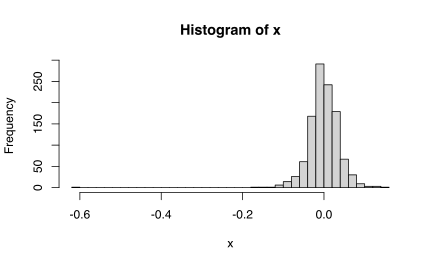
\includegraphics[width=0.7\linewidth]{Notas-Curso-Estadistica_files/figure-latex/unnamed-chunk-49-1} \end{center}

\begin{Shaded}
\begin{Highlighting}[]
\NormalTok{h_iqr <-}\StringTok{ }\FloatTok{1.06} \OperatorTok{*}\StringTok{ }\KeywordTok{min}\NormalTok{(s, }\KeywordTok{IQR}\NormalTok{(x)}\OperatorTok{/}\FloatTok{1.34}\NormalTok{) }\OperatorTok{*}\StringTok{ }\NormalTok{n}\OperatorTok{^}\NormalTok{(}\OperatorTok{-}\DecValTok{1}\OperatorTok{/}\DecValTok{5}\NormalTok{)}

\NormalTok{h <-}\StringTok{ }\NormalTok{h_iqr}

\NormalTok{n_bins <-}\StringTok{ }\KeywordTok{floor}\NormalTok{(}\KeywordTok{diff}\NormalTok{(}\KeywordTok{range}\NormalTok{(x))}\OperatorTok{/}\NormalTok{h)}
\NormalTok{f_hist <-}\StringTok{ }\KeywordTok{hist}\NormalTok{(x, }\DataTypeTok{breaks =}\NormalTok{ n_bins, }\DataTypeTok{plot =} \OtherTok{FALSE}\NormalTok{)}
\NormalTok{f_epa <-}\StringTok{ }\KeywordTok{as.data.frame}\NormalTok{(}\KeywordTok{bkde}\NormalTok{(x, }\DataTypeTok{kernel =} \StringTok{"epa"}\NormalTok{, }\DataTypeTok{bandwidth =}\NormalTok{ h))}

\KeywordTok{ggplot}\NormalTok{(x_df, }\KeywordTok{aes}\NormalTok{(x)) }\OperatorTok{+}\StringTok{ }\KeywordTok{geom_histogram}\NormalTok{(}\KeywordTok{aes}\NormalTok{(}\DataTypeTok{y =}\NormalTok{ ..density..), }
    \DataTypeTok{binwidth =}\NormalTok{ h, }\DataTypeTok{col =} \StringTok{"black"}\NormalTok{, }\DataTypeTok{fill =} \StringTok{"white"}\NormalTok{) }\OperatorTok{+}\StringTok{ }
\StringTok{    }\KeywordTok{stat_function}\NormalTok{(}\DataTypeTok{fun =}\NormalTok{ dnorm, }\DataTypeTok{args =} \KeywordTok{list}\NormalTok{(}\DataTypeTok{mean =}\NormalTok{ mu, }
        \DataTypeTok{sd =}\NormalTok{ sigma), }\DataTypeTok{color =} \StringTok{"red"}\NormalTok{) }\OperatorTok{+}\StringTok{ }\KeywordTok{geom_line}\NormalTok{(}\DataTypeTok{data =}\NormalTok{ f_epa, }
    \KeywordTok{aes}\NormalTok{(x, y), }\DataTypeTok{color =} \StringTok{"blue"}\NormalTok{) }\OperatorTok{+}\StringTok{ }\KeywordTok{theme_minimal}\NormalTok{(}\DataTypeTok{base_size =} \DecValTok{20}\NormalTok{)}
\end{Highlighting}
\end{Shaded}

\begin{center}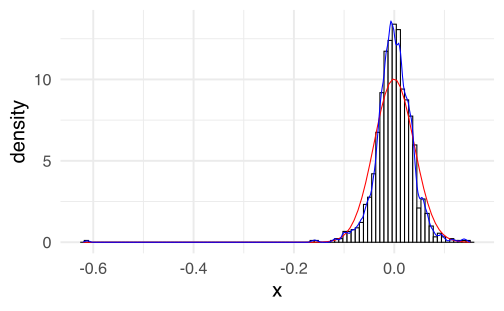
\includegraphics[width=0.7\linewidth]{Notas-Curso-Estadistica_files/figure-latex/unnamed-chunk-50-1} \end{center}

Una librería más especializada es \texttt{np} (non-parametric).

\begin{Shaded}
\begin{Highlighting}[]
\KeywordTok{library}\NormalTok{(np)}

\NormalTok{x.eval <-}\StringTok{ }\KeywordTok{seq}\NormalTok{(}\OperatorTok{-}\FloatTok{0.2}\NormalTok{, }\FloatTok{0.2}\NormalTok{, }\DataTypeTok{length.out =} \DecValTok{200}\NormalTok{)}

\NormalTok{h_normal_np <-}\StringTok{ }\KeywordTok{npudensbw}\NormalTok{(}\DataTypeTok{dat =}\NormalTok{ x, }\DataTypeTok{bwmethod =} \StringTok{"normal-reference"}\NormalTok{)}

\NormalTok{dens.ksum <-}\StringTok{ }\KeywordTok{npksum}\NormalTok{(}\DataTypeTok{txdat =}\NormalTok{ x, }\DataTypeTok{exdat =}\NormalTok{ x.eval, }\DataTypeTok{bws =}\NormalTok{ h_normal_np}\OperatorTok{$}\NormalTok{bw)}\OperatorTok{$}\NormalTok{ksum}\OperatorTok{/}\NormalTok{(n }\OperatorTok{*}\StringTok{ }
\StringTok{    }\NormalTok{h_normal_np}\OperatorTok{$}\NormalTok{bw[}\DecValTok{1}\NormalTok{])}

\NormalTok{dens.ksum.df <-}\StringTok{ }\KeywordTok{data.frame}\NormalTok{(}\DataTypeTok{x =}\NormalTok{ x.eval, }\DataTypeTok{y =}\NormalTok{ dens.ksum)}

\KeywordTok{ggplot}\NormalTok{(x_df, }\KeywordTok{aes}\NormalTok{(x)) }\OperatorTok{+}\StringTok{ }\KeywordTok{geom_histogram}\NormalTok{(}\KeywordTok{aes}\NormalTok{(}\DataTypeTok{y =}\NormalTok{ ..density..), }
    \DataTypeTok{binwidth =}\NormalTok{ h_normal_np}\OperatorTok{$}\NormalTok{bw, }\DataTypeTok{col =} \StringTok{"black"}\NormalTok{, }\DataTypeTok{fill =} \StringTok{"white"}\NormalTok{) }\OperatorTok{+}\StringTok{ }
\StringTok{    }\KeywordTok{stat_function}\NormalTok{(}\DataTypeTok{fun =}\NormalTok{ dnorm, }\DataTypeTok{args =} \KeywordTok{list}\NormalTok{(}\DataTypeTok{mean =}\NormalTok{ mu, }
        \DataTypeTok{sd =}\NormalTok{ sigma), }\DataTypeTok{color =} \StringTok{"red"}\NormalTok{) }\OperatorTok{+}\StringTok{ }\KeywordTok{geom_line}\NormalTok{(}\DataTypeTok{data =}\NormalTok{ dens.ksum.df, }
    \KeywordTok{aes}\NormalTok{(x, y), }\DataTypeTok{color =} \StringTok{"blue"}\NormalTok{) }\OperatorTok{+}\StringTok{ }\KeywordTok{theme_minimal}\NormalTok{(}\DataTypeTok{base_size =} \DecValTok{20}\NormalTok{)}
\end{Highlighting}
\end{Shaded}

\begin{center}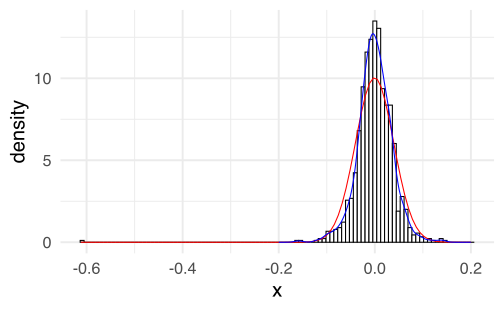
\includegraphics[width=0.7\linewidth]{Notas-Curso-Estadistica_files/figure-latex/unnamed-chunk-51-1} \end{center}

\hypertarget{validaciuxf3n-cruzada-1}{%
\subsection{Validación cruzada}\label{validaciuxf3n-cruzada-1}}

La forma que vimos en clase es la de validación cruzada por mínimos
cuadrados``least-square cross validation'' la cual se puede ejecutar
con este comando.

\begin{Shaded}
\begin{Highlighting}[]
\NormalTok{h_cv_np_ls <-}\StringTok{ }\KeywordTok{npudensbw}\NormalTok{(}\DataTypeTok{dat =}\NormalTok{ x, }\DataTypeTok{bwmethod =} \StringTok{"cv.ls"}\NormalTok{, }
    \DataTypeTok{ckertype =} \StringTok{"epa"}\NormalTok{, }\DataTypeTok{ckerorder =} \DecValTok{2}\NormalTok{)}
\end{Highlighting}
\end{Shaded}

\begin{verbatim}
## Multistart 1 of 1 |Multistart 1 of 1 |Multistart 1 of 1 |Multistart 1 of 1 /Multistart 1 of 1 |Multistart 1 of 1 |                   
\end{verbatim}

\begin{Shaded}
\begin{Highlighting}[]
\NormalTok{dens.np <-}\StringTok{ }\KeywordTok{npudens}\NormalTok{(h_cv_np_ls)}

\KeywordTok{plot}\NormalTok{(dens.np, }\DataTypeTok{type =} \StringTok{"b"}\NormalTok{)}
\end{Highlighting}
\end{Shaded}

\begin{center}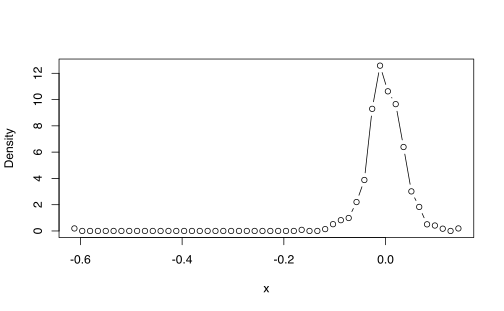
\includegraphics[width=0.7\linewidth]{Notas-Curso-Estadistica_files/figure-latex/unnamed-chunk-52-1} \end{center}

\begin{Shaded}
\begin{Highlighting}[]
\NormalTok{dens.np.df <-}\StringTok{ }\KeywordTok{data.frame}\NormalTok{(}\DataTypeTok{x =}\NormalTok{ dens.np}\OperatorTok{$}\NormalTok{eval[, }\DecValTok{1}\NormalTok{], }\DataTypeTok{y =}\NormalTok{ dens.np}\OperatorTok{$}\NormalTok{dens)}

\KeywordTok{ggplot}\NormalTok{(x_df, }\KeywordTok{aes}\NormalTok{(x)) }\OperatorTok{+}\StringTok{ }\KeywordTok{geom_histogram}\NormalTok{(}\KeywordTok{aes}\NormalTok{(}\DataTypeTok{y =}\NormalTok{ ..density..), }
    \DataTypeTok{binwidth =}\NormalTok{ h_cv_np_ls}\OperatorTok{$}\NormalTok{bw, }\DataTypeTok{col =} \StringTok{"black"}\NormalTok{, }\DataTypeTok{fill =} \StringTok{"white"}\NormalTok{) }\OperatorTok{+}\StringTok{ }
\StringTok{    }\KeywordTok{stat_function}\NormalTok{(}\DataTypeTok{fun =}\NormalTok{ dnorm, }\DataTypeTok{args =} \KeywordTok{list}\NormalTok{(}\DataTypeTok{mean =}\NormalTok{ mu, }
        \DataTypeTok{sd =}\NormalTok{ sigma), }\DataTypeTok{color =} \StringTok{"red"}\NormalTok{) }\OperatorTok{+}\StringTok{ }\KeywordTok{geom_line}\NormalTok{(}\DataTypeTok{data =}\NormalTok{ dens.np.df, }
    \KeywordTok{aes}\NormalTok{(x, y), }\DataTypeTok{color =} \StringTok{"blue"}\NormalTok{) }\OperatorTok{+}\StringTok{ }\KeywordTok{theme_minimal}\NormalTok{(}\DataTypeTok{base_size =} \DecValTok{20}\NormalTok{)}
\end{Highlighting}
\end{Shaded}

\begin{center}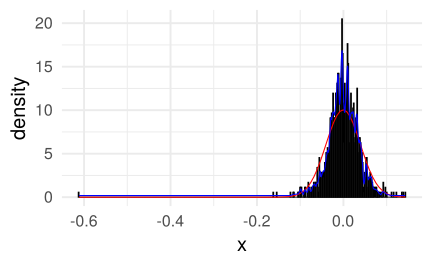
\includegraphics[width=0.7\linewidth]{Notas-Curso-Estadistica_files/figure-latex/unnamed-chunk-53-1} \end{center}

\hypertarget{temas-adicionales}{%
\subsection{Temas adicionales}\label{temas-adicionales}}

** Reducción del sesgo **
Como lo mencionamos en el texto, una forma de mejorar el sesgo en la estimación es suponer que la función de densidad es más veces diferenciable.

Esto se logra asumiendo que el Kernel es más veces diferenciable.

\begin{Shaded}
\begin{Highlighting}[]
\NormalTok{h_cv_np_ls <-}\StringTok{ }\KeywordTok{npudensbw}\NormalTok{(}\DataTypeTok{dat =}\NormalTok{ x, }\DataTypeTok{bwmethod =} \StringTok{"cv.ls"}\NormalTok{, }
    \DataTypeTok{ckertype =} \StringTok{"epa"}\NormalTok{, }\DataTypeTok{ckerorder =} \DecValTok{4}\NormalTok{)}
\end{Highlighting}
\end{Shaded}

\begin{verbatim}
## Multistart 1 of 1 |Multistart 1 of 1 |Multistart 1 of 1 |Multistart 1 of 1 /Multistart 1 of 1 |Multistart 1 of 1 |                   
\end{verbatim}

\begin{Shaded}
\begin{Highlighting}[]
\NormalTok{dens.np <-}\StringTok{ }\KeywordTok{npudens}\NormalTok{(h_cv_np_ls)}

\KeywordTok{plot}\NormalTok{(dens.np, }\DataTypeTok{type =} \StringTok{"b"}\NormalTok{, }\DataTypeTok{lwd =} \DecValTok{2}\NormalTok{)}
\end{Highlighting}
\end{Shaded}

\begin{center}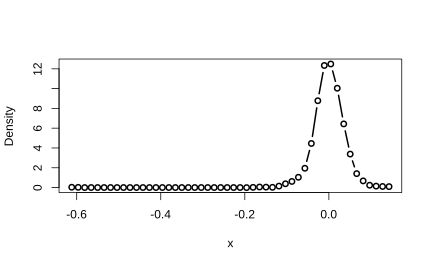
\includegraphics[width=0.7\linewidth]{Notas-Curso-Estadistica_files/figure-latex/unnamed-chunk-54-1} \end{center}

\begin{Shaded}
\begin{Highlighting}[]
\NormalTok{dens.np.df <-}\StringTok{ }\KeywordTok{data.frame}\NormalTok{(}\DataTypeTok{x =}\NormalTok{ dens.np}\OperatorTok{$}\NormalTok{eval[, }\DecValTok{1}\NormalTok{], }\DataTypeTok{y =}\NormalTok{ dens.np}\OperatorTok{$}\NormalTok{dens)}

\KeywordTok{ggplot}\NormalTok{(x_df, }\KeywordTok{aes}\NormalTok{(x)) }\OperatorTok{+}\StringTok{ }\KeywordTok{geom_histogram}\NormalTok{(}\KeywordTok{aes}\NormalTok{(}\DataTypeTok{y =}\NormalTok{ ..density..), }
    \DataTypeTok{binwidth =}\NormalTok{ h_cv_np_ls}\OperatorTok{$}\NormalTok{bw, }\DataTypeTok{col =} \StringTok{"black"}\NormalTok{, }\DataTypeTok{fill =} \StringTok{"white"}\NormalTok{) }\OperatorTok{+}\StringTok{ }
\StringTok{    }\KeywordTok{stat_function}\NormalTok{(}\DataTypeTok{fun =}\NormalTok{ dnorm, }\DataTypeTok{args =} \KeywordTok{list}\NormalTok{(}\DataTypeTok{mean =}\NormalTok{ mu, }
        \DataTypeTok{sd =}\NormalTok{ sigma), }\DataTypeTok{color =} \StringTok{"red"}\NormalTok{) }\OperatorTok{+}\StringTok{ }\KeywordTok{geom_line}\NormalTok{(}\DataTypeTok{data =}\NormalTok{ dens.np.df, }
    \KeywordTok{aes}\NormalTok{(x, y), }\DataTypeTok{color =} \StringTok{"blue"}\NormalTok{) }\OperatorTok{+}\StringTok{ }\KeywordTok{theme_minimal}\NormalTok{(}\DataTypeTok{base_size =} \DecValTok{20}\NormalTok{)}
\end{Highlighting}
\end{Shaded}

\begin{center}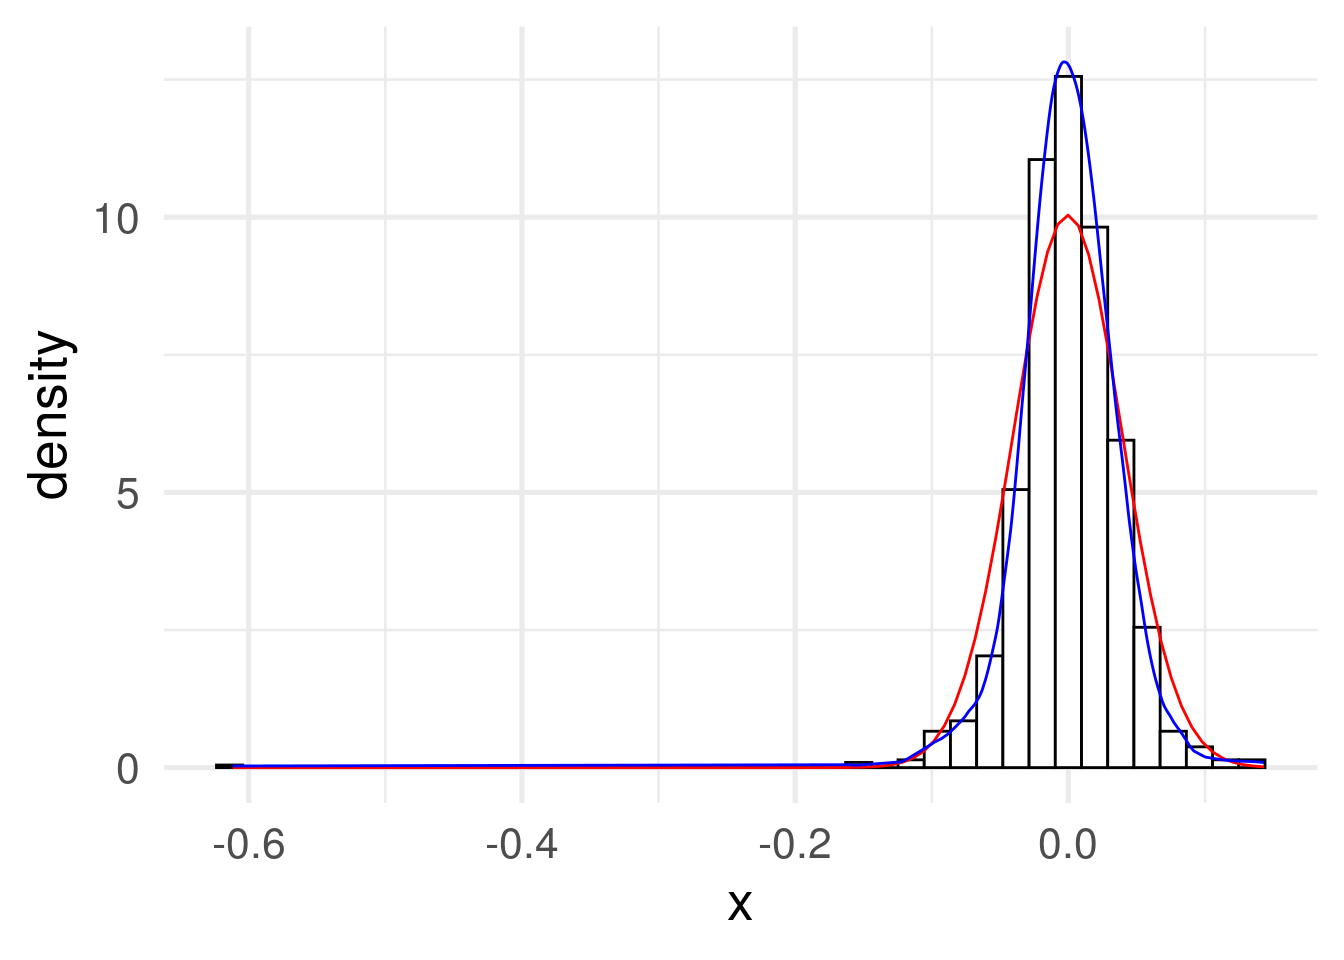
\includegraphics[width=0.7\linewidth]{Notas-Curso-Estadistica_files/figure-latex/unnamed-chunk-55-1} \end{center}

\textbf{Otra forma de estimar el ancho de banda} Otra forma de estimar ancho de bandas óptimos es usando máxima verosimilitud. Les dejo de tarea revisar la sección 1.1 del artículo de \autocite{Hall1987} para entender su estructura.

\begin{Shaded}
\begin{Highlighting}[]
\NormalTok{h_cv_np_ml <-}\StringTok{ }\KeywordTok{npudensbw}\NormalTok{(}\DataTypeTok{dat =}\NormalTok{ x, }\DataTypeTok{bwmethod =} \StringTok{"cv.ml"}\NormalTok{, }
    \DataTypeTok{ckertype =} \StringTok{"epanechnikov"}\NormalTok{)}
\end{Highlighting}
\end{Shaded}

\begin{verbatim}
## Multistart 1 of 1 |Multistart 1 of 1 |Multistart 1 of 1 |Multistart 1 of 1 /Multistart 1 of 1 |Multistart 1 of 1 |                   
\end{verbatim}

\begin{Shaded}
\begin{Highlighting}[]
\NormalTok{dens.np <-}\StringTok{ }\KeywordTok{npudens}\NormalTok{(h_cv_np_ml)}

\KeywordTok{plot}\NormalTok{(dens.np, }\DataTypeTok{type =} \StringTok{"b"}\NormalTok{)}
\end{Highlighting}
\end{Shaded}

\begin{center}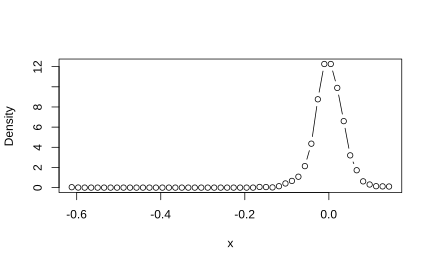
\includegraphics[width=0.7\linewidth]{Notas-Curso-Estadistica_files/figure-latex/unnamed-chunk-56-1} \end{center}

\begin{Shaded}
\begin{Highlighting}[]
\NormalTok{dens.np.df <-}\StringTok{ }\KeywordTok{data.frame}\NormalTok{(}\DataTypeTok{x =}\NormalTok{ dens.np}\OperatorTok{$}\NormalTok{eval[, }\DecValTok{1}\NormalTok{], }\DataTypeTok{y =}\NormalTok{ dens.np}\OperatorTok{$}\NormalTok{dens)}

\KeywordTok{ggplot}\NormalTok{(x_df, }\KeywordTok{aes}\NormalTok{(x)) }\OperatorTok{+}\StringTok{ }\KeywordTok{geom_histogram}\NormalTok{(}\KeywordTok{aes}\NormalTok{(}\DataTypeTok{y =}\NormalTok{ ..density..), }
    \DataTypeTok{binwidth =}\NormalTok{ h_cv_np_ml}\OperatorTok{$}\NormalTok{bw, }\DataTypeTok{col =} \StringTok{"black"}\NormalTok{, }\DataTypeTok{fill =} \StringTok{"white"}\NormalTok{) }\OperatorTok{+}\StringTok{ }
\StringTok{    }\KeywordTok{stat_function}\NormalTok{(}\DataTypeTok{fun =}\NormalTok{ dnorm, }\DataTypeTok{args =} \KeywordTok{list}\NormalTok{(}\DataTypeTok{mean =}\NormalTok{ mu, }
        \DataTypeTok{sd =}\NormalTok{ sigma), }\DataTypeTok{color =} \StringTok{"red"}\NormalTok{) }\OperatorTok{+}\StringTok{ }\KeywordTok{geom_line}\NormalTok{(}\DataTypeTok{data =}\NormalTok{ dens.np.df, }
    \KeywordTok{aes}\NormalTok{(x, y), }\DataTypeTok{color =} \StringTok{"blue"}\NormalTok{) }\OperatorTok{+}\StringTok{ }\KeywordTok{theme_minimal}\NormalTok{(}\DataTypeTok{base_size =} \DecValTok{20}\NormalTok{)}
\end{Highlighting}
\end{Shaded}

\begin{center}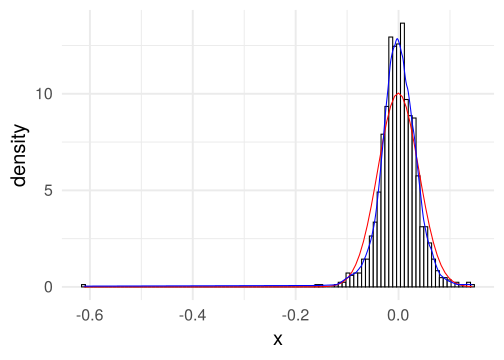
\includegraphics[width=0.7\linewidth]{Notas-Curso-Estadistica_files/figure-latex/unnamed-chunk-57-1} \end{center}

\begin{Shaded}
\begin{Highlighting}[]
\NormalTok{h_cv_np_ml <-}\StringTok{ }\KeywordTok{npudensbw}\NormalTok{(}\DataTypeTok{dat =}\NormalTok{ x, }\DataTypeTok{bwmethod =} \StringTok{"cv.ml"}\NormalTok{, }
    \DataTypeTok{ckertype =} \StringTok{"epanechnikov"}\NormalTok{, }\DataTypeTok{ckerorder =} \DecValTok{4}\NormalTok{)}
\end{Highlighting}
\end{Shaded}

\begin{verbatim}
## Multistart 1 of 1 |Multistart 1 of 1 |Multistart 1 of 1 |Multistart 1 of 1 /Multistart 1 of 1 |Multistart 1 of 1 |                   
\end{verbatim}

\begin{Shaded}
\begin{Highlighting}[]
\NormalTok{dens.np <-}\StringTok{ }\KeywordTok{npudens}\NormalTok{(h_cv_np_ml)}

\KeywordTok{plot}\NormalTok{(dens.np, }\DataTypeTok{type =} \StringTok{"b"}\NormalTok{)}
\end{Highlighting}
\end{Shaded}

\begin{center}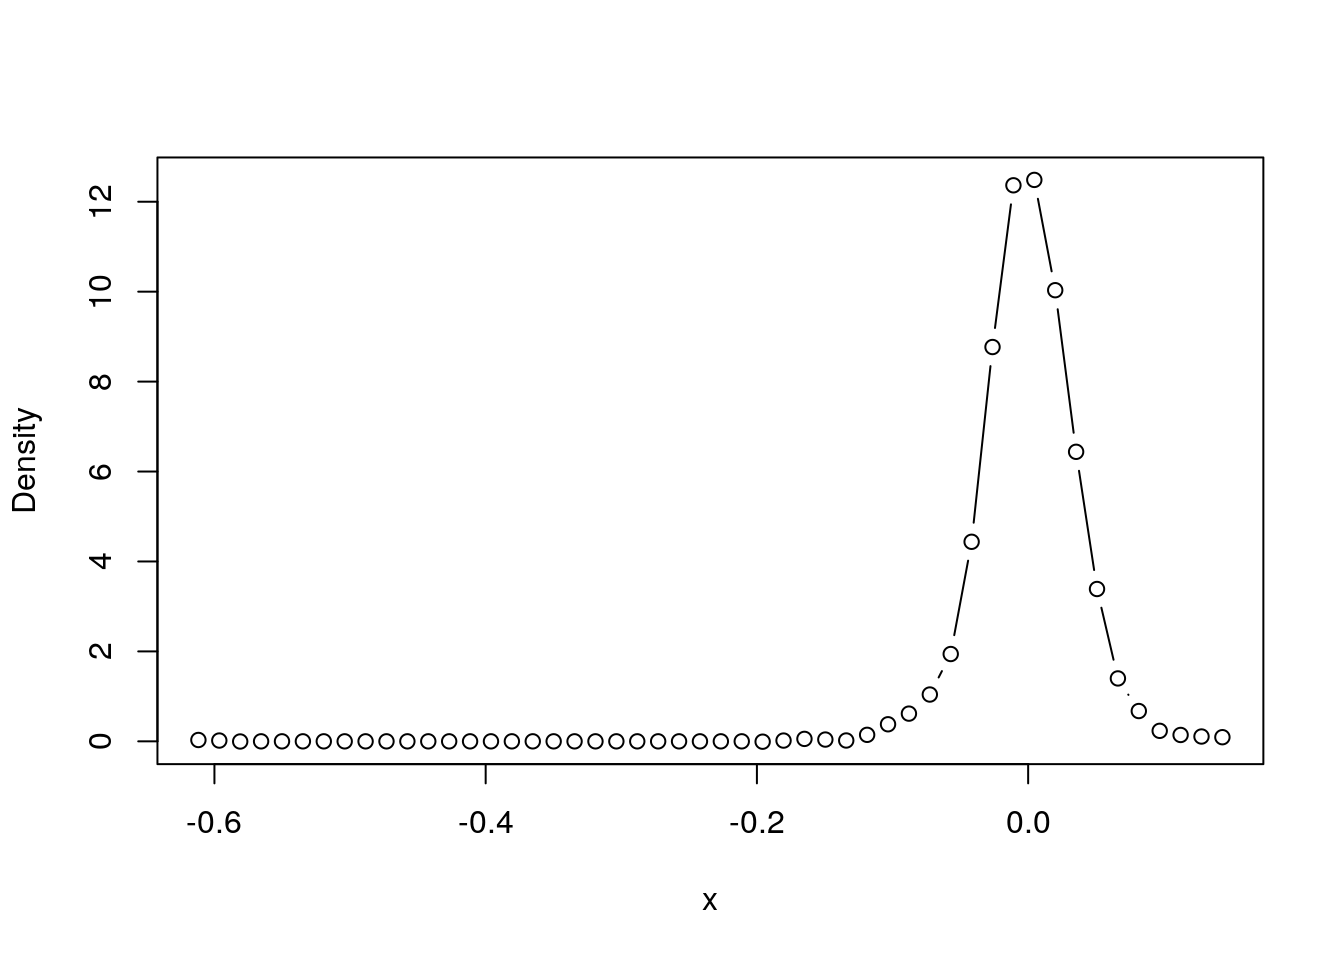
\includegraphics[width=0.7\linewidth]{Notas-Curso-Estadistica_files/figure-latex/unnamed-chunk-58-1} \end{center}

\begin{Shaded}
\begin{Highlighting}[]
\NormalTok{dens.np.df <-}\StringTok{ }\KeywordTok{data.frame}\NormalTok{(}\DataTypeTok{x =}\NormalTok{ dens.np}\OperatorTok{$}\NormalTok{eval[, }\DecValTok{1}\NormalTok{], }\DataTypeTok{y =}\NormalTok{ dens.np}\OperatorTok{$}\NormalTok{dens)}

\KeywordTok{ggplot}\NormalTok{(x_df, }\KeywordTok{aes}\NormalTok{(x)) }\OperatorTok{+}\StringTok{ }\KeywordTok{geom_histogram}\NormalTok{(}\KeywordTok{aes}\NormalTok{(}\DataTypeTok{y =}\NormalTok{ ..density..), }
    \DataTypeTok{binwidth =}\NormalTok{ h_cv_np_ml}\OperatorTok{$}\NormalTok{bw, }\DataTypeTok{col =} \StringTok{"black"}\NormalTok{, }\DataTypeTok{fill =} \StringTok{"white"}\NormalTok{) }\OperatorTok{+}\StringTok{ }
\StringTok{    }\KeywordTok{stat_function}\NormalTok{(}\DataTypeTok{fun =}\NormalTok{ dnorm, }\DataTypeTok{args =} \KeywordTok{list}\NormalTok{(}\DataTypeTok{mean =}\NormalTok{ mu, }
        \DataTypeTok{sd =}\NormalTok{ sigma), }\DataTypeTok{color =} \StringTok{"red"}\NormalTok{) }\OperatorTok{+}\StringTok{ }\KeywordTok{geom_line}\NormalTok{(}\DataTypeTok{data =}\NormalTok{ dens.np.df, }
    \KeywordTok{aes}\NormalTok{(x, y), }\DataTypeTok{color =} \StringTok{"blue"}\NormalTok{) }\OperatorTok{+}\StringTok{ }\KeywordTok{theme_minimal}\NormalTok{(}\DataTypeTok{base_size =} \DecValTok{20}\NormalTok{)}
\end{Highlighting}
\end{Shaded}

\begin{center}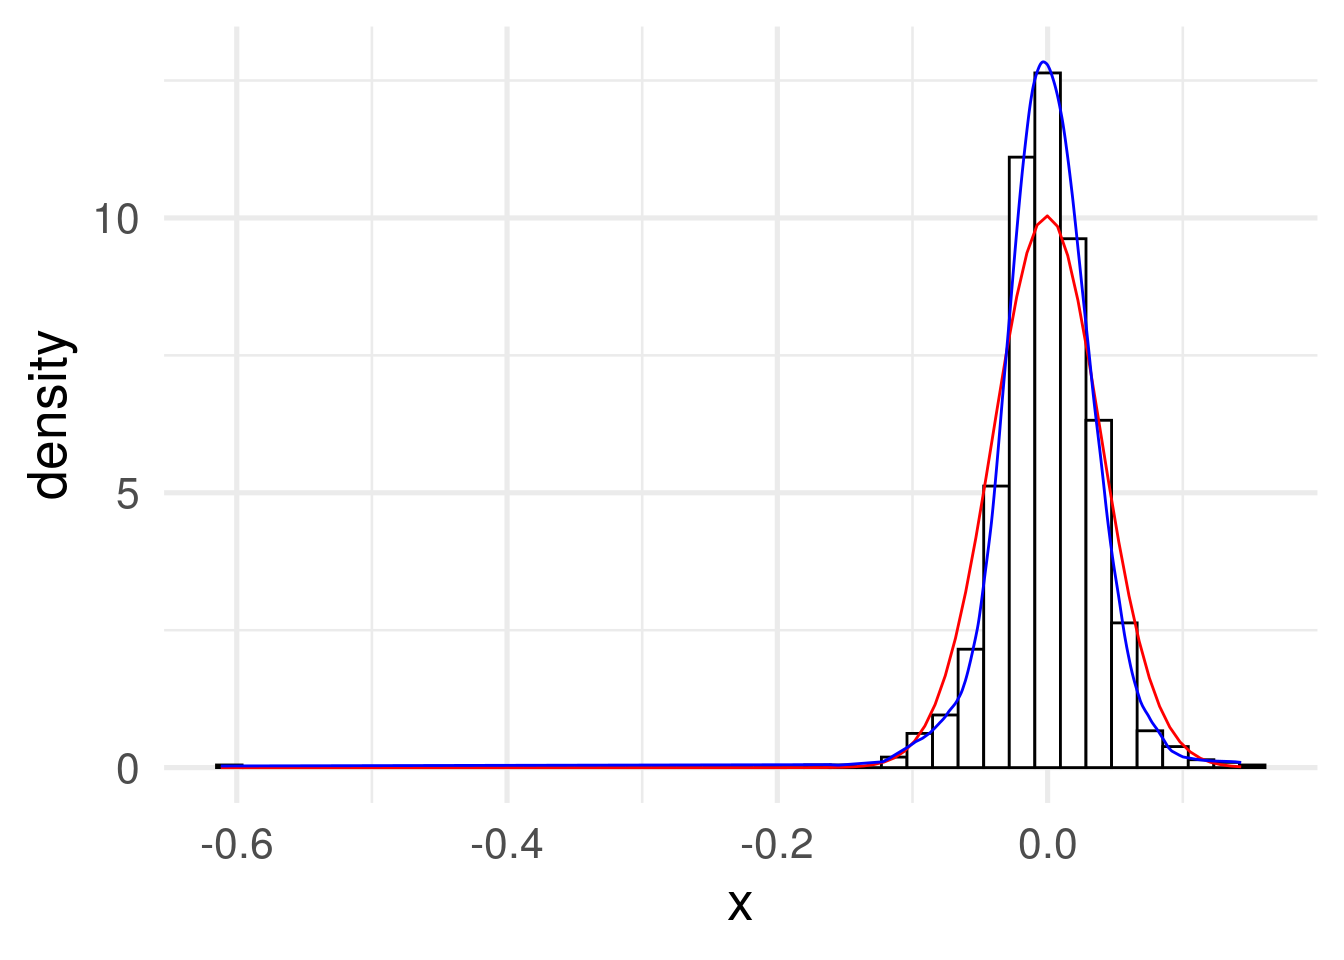
\includegraphics[width=0.7\linewidth]{Notas-Curso-Estadistica_files/figure-latex/unnamed-chunk-59-1} \end{center}

\begin{Shaded}
\begin{Highlighting}[]
\NormalTok{fani <-}\StringTok{ }\KeywordTok{tibble}\NormalTok{()}

\ControlFlowTok{for}\NormalTok{ (b }\ControlFlowTok{in} \KeywordTok{seq}\NormalTok{(}\FloatTok{0.001}\NormalTok{, }\FloatTok{0.05}\NormalTok{, }\DataTypeTok{length.out =} \DecValTok{40}\NormalTok{)) \{}
\NormalTok{    f <-}\StringTok{ }\KeywordTok{npudens}\NormalTok{(}\DataTypeTok{tdat =}\NormalTok{ x, }\DataTypeTok{ckertype =} \StringTok{"epanechnikov"}\NormalTok{, }
        \DataTypeTok{bandwidth.compute =} \OtherTok{FALSE}\NormalTok{, }\DataTypeTok{bws =}\NormalTok{ b)}
\NormalTok{    fani <-}\StringTok{ }\NormalTok{fani }\OperatorTok\StringTok{ }\KeywordTok{bind_rows}\NormalTok{(}\KeywordTok{tibble}\NormalTok{(}\DataTypeTok{xreal =} \KeywordTok{sort}\NormalTok{(x), }
        \DataTypeTok{x =}\NormalTok{ f}\OperatorTok{$}\NormalTok{eval}\OperatorTok{$}\NormalTok{x, }\DataTypeTok{y =}\NormalTok{ f}\OperatorTok{$}\NormalTok{dens, }\DataTypeTok{bw =}\NormalTok{ b))}
\NormalTok{\}}

\KeywordTok{ggplot}\NormalTok{(}\DataTypeTok{data =}\NormalTok{ fani) }\OperatorTok{+}\StringTok{ }\KeywordTok{geom_line}\NormalTok{(}\KeywordTok{aes}\NormalTok{(x, y), }\DataTypeTok{color =} \StringTok{"blue"}\NormalTok{) }\OperatorTok{+}\StringTok{ }
\StringTok{    }\KeywordTok{labs}\NormalTok{(}\DataTypeTok{title =} \KeywordTok{paste0}\NormalTok{(}\StringTok{"Ancho de banda = \{closest_state\}"}\NormalTok{)) }\OperatorTok{+}\StringTok{ }
\StringTok{    }\KeywordTok{theme_minimal}\NormalTok{(}\DataTypeTok{base_size =} \DecValTok{20}\NormalTok{) }\OperatorTok{+}\StringTok{ }\KeywordTok{transition_states}\NormalTok{(bw) }\OperatorTok{+}\StringTok{ }
\StringTok{    }\KeywordTok{view_follow}\NormalTok{()}

\CommentTok{# anim_save('manual_figure/bandwidth-animation-np.gif')}
\end{Highlighting}
\end{Shaded}

\BeginKnitrBlock{exercise}
\protect\hypertarget{exr:unnamed-chunk-61}{}{\label{exr:unnamed-chunk-61} }Implementar el intervalo confianza visto en clase para estimadores de densidades por núcleos y visualizarlo de en ggplot.

\textbf{Si se atreven: ¿Se podría hacer una versión animada de ese gráfico para visualizar el significado real de este el intervalo de confianza?}
\EndKnitrBlock{exercise}

\hypertarget{ejercicios}{%
\section{Ejercicios}\label{ejercicios}}

Del libro de \autocite{Hardle2004} hagan los siguientes ejercicios

\begin{enumerate}
\def\labelenumi{\arabic{enumi}.}
\tightlist
\item
  \textbf{Sección 2:} 1, 2, 3, 5, 7, 14
\item
  \textbf{Sección 3:} 4, 8, 10, 11, 16,
\end{enumerate}

\hypertarget{jacknife-y-bootstrap}{%
\chapter{Jacknife y Bootstrap}\label{jacknife-y-bootstrap}}

Suponga que se quiere estimar un intervalo de confianza para la media
\(\mu\) desconocida de un conjunto de datos \(X_{1},\ldots, X_{n}\)
que tiene distribución \(\mathcal{N}\left(\mu ,\sigma^{2}\right)\).

Primero se conoce que

\begin{equation*}
\sqrt{n}\left( \hat{\mu} - \mu \right)
\xrightarrow{\mathcal{L}} \mathcal{N}\left(0,\sigma^{2}\right),
\end{equation*}

y esto nos permite escribir el intervalo de confianza como

\begin{equation*}
\left[ \hat{\mu} - \hat{\sigma}z_{1-\frac{\alpha}{2}} ,
\hat{\mu} + \hat{\sigma}z_{1-\frac{\alpha}{2}}\right]
\end{equation*}

donde \(z_{1-\frac{\alpha}{2}}\) es el cuantil \(1-\frac{\alpha}{2}\)
de una normal estándar.

La expresión anterior es posible ya que el supuesto es que la
distribución de \(\hat{\theta}\) es normal.

\BeginKnitrBlock{remark}
\iffalse{} {Nota: } \fi{}¿Qué pasaría si este supuesto es falso o al menos no conocemos la
distribución de \(\hat{\theta}\)?

¿Cómo podemos encontrar ese intervalo de confianza?
\EndKnitrBlock{remark}

\BeginKnitrBlock{remark}
\iffalse{} {Nota: } \fi{}Para una muestra fija, el estimador anterior \(\hat{\mu}\)
solamente un valor. No se conoce la distribución de \(\hat{\mu}\). Lo
único que se puede estimar son valores puntuales como la media,
varianza, mediana, etc, pero no sabemos nada de su distribución.
\EndKnitrBlock{remark}

\hypertarget{caso-concreto}{%
\section{Caso concreto}\label{caso-concreto}}

Suponga que tenemos la siguiente tabla de datos, que representa una
muestra de tiempos y distancias de viajes en Atlanta.

Cargamos la base de la siguiente forma:

\begin{Shaded}
\begin{Highlighting}[]
\NormalTok{CommuteAtlanta <-}\StringTok{ }\KeywordTok{read.csv2}\NormalTok{(}\StringTok{"data/CommuteAtlanta.csv"}\NormalTok{)}
\end{Highlighting}
\end{Shaded}

\begin{tabular}{l|r|r|r|l}
\hline
City & Age & Distance & Time & Sex\\
\hline
Atlanta & 19 & 10 & 15 & M\\
\hline
Atlanta & 55 & 45 & 60 & M\\
\hline
Atlanta & 48 & 12 & 45 & M\\
\hline
Atlanta & 45 & 4 & 10 & F\\
\hline
Atlanta & 48 & 15 & 30 & F\\
\hline
Atlanta & 43 & 33 & 60 & M\\
\hline
\end{tabular}

Para este ejemplo tomaremos la variable \texttt{Time} que la
llamaremos \texttt{x} para ser más breves. En este caso note que

\begin{Shaded}
\begin{Highlighting}[]
\NormalTok{x <-}\StringTok{ }\NormalTok{CommuteAtlanta}\OperatorTok{$}\NormalTok{Time}
\end{Highlighting}
\end{Shaded}

La media es 29.11 y su varianza 429.2483968. Para efectos de lo que sigue, asignaremos la varianza a la variable \(T_n\)

\begin{Shaded}
\begin{Highlighting}[]
\NormalTok{Tn <-}\StringTok{ }\KeywordTok{var}\NormalTok{(x)}
\end{Highlighting}
\end{Shaded}

A partir de estos dos valores, ¿Cuál sería un intervalo de confianza
para la media?

Note que esta pregunta es difícil ya que no tenemos ningún tipo de
información adicional.

Las dos técnicas que veremos a continuación nos permitirán extraer
\emph{información adicional} de la muestra.

\BeginKnitrBlock{remark}
\iffalse{} {Nota: } \fi{}Para efectos de este capítulo, llamaremos \(T_{n}=T\left(  X_{1},\ldots,X_{n}\right)\) al estadístico formado por la muestra de
los \(X_{i}\)'s.
\EndKnitrBlock{remark}

\hypertarget{jacknife}{%
\section{Jacknife}\label{jacknife}}

Esta técnica fue propuesta por \cite{Quenouille1949} y consiste en la
siguiente observación.

Se puede probar que muchos de los estimadores tiene la propiedad que

\begin{equation}
\operatorname{Sesgo}\left(T_{n}\right)=\frac{a}{n}+\frac{b}{n^{2}}+O\left(\frac{1}{n^{3}}\right)
\end{equation}

para algún \(a\) and \(b\).

Por ejemplo \(\sigma^{2}=\mathrm{Var}\left(X_{i}\right)\) y sea
\(\widehat{\sigma}_{n}^{2}=n^{-1} \sum_{i=1}^{n}\left(X_{i}-\right.\)
\(\bar{X})^{2}\). Entonces,

\begin{equation*}
\mathbb{E}\left(\widehat{\sigma}_{n}^{2}\right)=
\frac{n-1}{n}\sigma^{2}
\end{equation*}

por lo tanto

\begin{equation*}
\mathrm{Sesgo} = -\frac{\sigma^{2}}{n}
\end{equation*}

Por lo tanto en este caso \(a=-\sigma^{2}\) y \(b=0\).

Defina \(T_{(-i)}\) como el estimador \(T_{n}\) pero eliminando el
\(i\)-ésimo término.

Es claro que en este contexto, se tiene que

\begin{equation}
\operatorname{Sesgo}\left(T_{(-i)}\right)=\frac{a}{n-1}+\frac{b}{(n-1)^{2}}+O\left(\frac{1}{(n-1)^{3}}\right)
\end{equation}

\BeginKnitrBlock{exercise}
\protect\hypertarget{exr:unnamed-chunk-67}{}{\label{exr:unnamed-chunk-67} }Una forma fácil de construir los \(T_{(-i)}\) es primero replicando
la matriz de datos múltiple veces usando el producto de kronecker
\EndKnitrBlock{exercise}

\begin{Shaded}
\begin{Highlighting}[]
\NormalTok{n <-}\StringTok{ }\KeywordTok{length}\NormalTok{(x)}
\NormalTok{jackdf <-}\StringTok{ }\KeywordTok{kronecker}\NormalTok{(}\KeywordTok{matrix}\NormalTok{(}\DecValTok{1}\NormalTok{, }\DecValTok{1}\NormalTok{, n), x)}
\end{Highlighting}
\end{Shaded}

\begin{tabular}{r|r|r|r|r|r|r|r|r|r}
\hline
15 & 15 & 15 & 15 & 15 & 15 & 15 & 15 & 15 & 15\\
\hline
60 & 60 & 60 & 60 & 60 & 60 & 60 & 60 & 60 & 60\\
\hline
45 & 45 & 45 & 45 & 45 & 45 & 45 & 45 & 45 & 45\\
\hline
10 & 10 & 10 & 10 & 10 & 10 & 10 & 10 & 10 & 10\\
\hline
30 & 30 & 30 & 30 & 30 & 30 & 30 & 30 & 30 & 30\\
\hline
60 & 60 & 60 & 60 & 60 & 60 & 60 & 60 & 60 & 60\\
\hline
45 & 45 & 45 & 45 & 45 & 45 & 45 & 45 & 45 & 45\\
\hline
10 & 10 & 10 & 10 & 10 & 10 & 10 & 10 & 10 & 10\\
\hline
25 & 25 & 25 & 25 & 25 & 25 & 25 & 25 & 25 & 25\\
\hline
15 & 15 & 15 & 15 & 15 & 15 & 15 & 15 & 15 & 15\\
\hline
\end{tabular}

Y luego se elimina la diagonal

\begin{Shaded}
\begin{Highlighting}[]
\KeywordTok{diag}\NormalTok{(jackdf) <-}\StringTok{ }\OtherTok{NA}
\end{Highlighting}
\end{Shaded}

\begin{tabular}{r|r|r|r|r|r|r|r|r|r}
\hline
NA & 15 & 15 & 15 & 15 & 15 & 15 & 15 & 15 & 15\\
\hline
60 & NA & 60 & 60 & 60 & 60 & 60 & 60 & 60 & 60\\
\hline
45 & 45 & NA & 45 & 45 & 45 & 45 & 45 & 45 & 45\\
\hline
10 & 10 & 10 & NA & 10 & 10 & 10 & 10 & 10 & 10\\
\hline
30 & 30 & 30 & 30 & NA & 30 & 30 & 30 & 30 & 30\\
\hline
60 & 60 & 60 & 60 & 60 & NA & 60 & 60 & 60 & 60\\
\hline
45 & 45 & 45 & 45 & 45 & 45 & NA & 45 & 45 & 45\\
\hline
10 & 10 & 10 & 10 & 10 & 10 & 10 & NA & 10 & 10\\
\hline
25 & 25 & 25 & 25 & 25 & 25 & 25 & 25 & NA & 25\\
\hline
15 & 15 & 15 & 15 & 15 & 15 & 15 & 15 & 15 & NA\\
\hline
\end{tabular}

Cada columna contiene toda la muestra excepto el \(i\)-ésimo
elemento. Solo basta estimar la media de cada columna:

\begin{Shaded}
\begin{Highlighting}[]
\NormalTok{T_i <-}\StringTok{ }\KeywordTok{apply}\NormalTok{(jackdf, }\DecValTok{2}\NormalTok{, var, }\DataTypeTok{na.rm =} \OtherTok{TRUE}\NormalTok{)}
\end{Highlighting}
\end{Shaded}

\begin{tabular}{r}
\hline
x\\
\hline
429.7098\\
\hline
428.1905\\
\hline
429.6023\\
\hline
429.3756\\
\hline
430.1087\\
\hline
428.1905\\
\hline
429.6023\\
\hline
429.3756\\
\hline
430.0764\\
\hline
429.7098\\
\hline
\end{tabular}

Definamos el sesgo \emph{jackife} como

\begin{equation*}
b_{jack} = (n-1) (\overline{T}_{n} - T_{n})
\end{equation*}

donde
\begin{equation*}
\overline{T}_{n} = \frac{1}{n} \sum_{i=1}^{n} T_{(-i)}
\end{equation*}

\BeginKnitrBlock{exercise}
\protect\hypertarget{exr:unnamed-chunk-71}{}{\label{exr:unnamed-chunk-71} }En nuestro caso tendríamos lo siguiente:
\EndKnitrBlock{exercise}

\begin{Shaded}
\begin{Highlighting}[]
\NormalTok{(bjack <-}\StringTok{ }\NormalTok{(n }\OperatorTok{-}\StringTok{ }\DecValTok{1}\NormalTok{) }\OperatorTok{*}\StringTok{ }\NormalTok{(}\KeywordTok{mean}\NormalTok{(T_i) }\OperatorTok{-}\StringTok{ }\NormalTok{Tn))}
\end{Highlighting}
\end{Shaded}

\begin{verbatim}
## [1] 0
\end{verbatim}

Es decir, que los \texttt{T\_i} generan estimadores de \texttt{T\_n}
que contienen el mismo sesgo.

Observe que \(b_{jack}\) tiene la siguiente propiedad

\begin{align*}
\mathbb{E}\left(b_{\text {jack}}\right)
&= (n-1)\left(\mathbb{E}\left[\overline{T}_{n}\right] -
\mathbb{E}\left[T_{n}\right]\right) \\
&= (n-1)\left(\mathbb{E}\left[\overline{T}_{n}\right] - \theta +
\theta - \mathbb{E}\left[T_{n}\right]\right) \\
& =(n-1)\left(\mathrm{Sesgo} \left(\overline{T}_{n}\right)
-\mathrm{Sesgo}\left(T_{n}\right)\right) \\
& =(n-1)\left[\left(\frac{1}{n-1}
-\frac{1}{n}\right)
a+\left(\frac{1}{(n-1)^{2}}
-\frac{1}{n^{2}}\right) b+O\left(\frac{1}{n^{3}}\right)\right] \\
& =\frac{a}{n}
+\frac{(2 n-1) b}{n^{2}(n-1)}
+O\left(\frac{1}{n^{2}}\right) \\
& =\operatorname{Sesgo}\left(T_{n}\right)
+O\left(\frac{1}{n^{2}}\right)\\
\end{align*}

\BeginKnitrBlock{remark}
\iffalse{} {Nota: } \fi{}Es decir, en general, el estimador \(b_{\text{jack}}\) aproxima
correctamente \(\mathrm{Sesgo}\left( T_{n} \right)\) hasta con un
error del \(n^{-2}\).
\EndKnitrBlock{remark}

Podemos usar los \(T\_i\) para generar muestras adicionales para
estimar el parámetro \(\theta\).

En este caso defina el siguiente estimador:

\[
\widetilde{T}_{i}=n T_{n}-(n-1) T_{(-i)}.
\]

\BeginKnitrBlock{remark}
\iffalse{} {Nota: } \fi{}A \(\widetilde{T}_{i}\) se le llaman \textbf{pseudo-valores} y
representa el aporte o peso que tiene la variable \(X_{i}\) para
estimar \(T_{n}\).
\EndKnitrBlock{remark}

\BeginKnitrBlock{exercise}
\protect\hypertarget{exr:unnamed-chunk-75}{}{\label{exr:unnamed-chunk-75} }Usado un cálculo similar para el \(b_{jack}\) pruebe que

\[
\operatorname{Sesgo}\left(T_{\text {jack}
}\right)=-\frac{b}{n(n-1)}+O\left(\frac{1}{n^{2}}\right)=O\left(\frac{1}{n^{2}}\right).
\]

¿Qué conclusión se obtiene de este cálculo?
\EndKnitrBlock{exercise}

\BeginKnitrBlock{exercise}
\protect\hypertarget{exr:unnamed-chunk-76}{}{\label{exr:unnamed-chunk-76} }Los pseudo-valores se estiman de forma directa como,
\EndKnitrBlock{exercise}

\begin{Shaded}
\begin{Highlighting}[]
\NormalTok{pseudo <-}\StringTok{ }\NormalTok{n }\OperatorTok{*}\StringTok{ }\NormalTok{Tn }\OperatorTok{-}\StringTok{ }\NormalTok{(n }\OperatorTok{-}\StringTok{ }\DecValTok{1}\NormalTok{) }\OperatorTok{*}\StringTok{ }\NormalTok{T_i}

\NormalTok{pseudo[}\DecValTok{1}\OperatorTok{:}\DecValTok{10}\NormalTok{]}
\end{Highlighting}
\end{Shaded}

\begin{verbatim}
##  [1] 199.02972209 957.16225222 252.64417993 365.79679037  -0.06666345
##  [6] 957.16225222 252.64417993 365.79679037  16.09799519 199.02972209
\end{verbatim}

Lo importante acá es notar la similitud que tiene con los datos
reales,

\begin{Shaded}
\begin{Highlighting}[]
\KeywordTok{plot}\NormalTok{(}\DataTypeTok{x =}\NormalTok{ x, }\DataTypeTok{y =}\NormalTok{ pseudo)}
\end{Highlighting}
\end{Shaded}

\begin{center}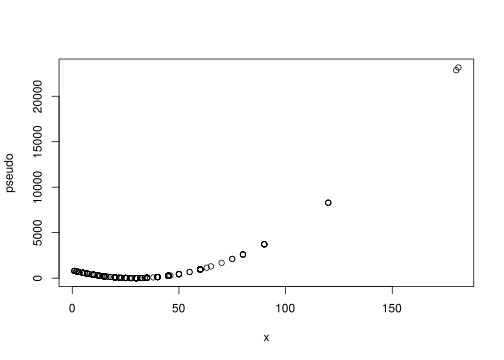
\includegraphics[width=0.7\linewidth]{Notas-Curso-Estadistica_files/figure-latex/unnamed-chunk-78-1} \end{center}

Con estos pseudo-valores, es posible estimar la media y la varianza de
\(T_{n}\) con sus respectivos estimadores:

\[
T_{\text {jack }}=\frac{1}{n} \sum_{i=1}^{n} \widetilde{T}_{i}
\]

donde

\[
v_{jack}=\frac{\sum_{i=1}^{n}\left(\widetilde{T}_{i}-\frac{1}{n}
\sum_{i=1}^{n} \widetilde{T}_{i}\right)^{2}}{n(n-1)}.
\]

\BeginKnitrBlock{remark}
\iffalse{} {Nota: } \fi{}
Sin embargo, se puede demostrar fácilmente que se pueden usar
pseudovalores para construir una prueba normal de hipótesis. Dado que
cada pseudovalor es independiente e idénticamente distribuido (iid),
se deduce que su promedio se ajusta a una distribución normal a medida
que el tamaño de la muestra aumenta. El promedio de los pseudovalores
es solo \(T_ {jack}\) y el valor esperado de ese promedio, debido a la
construcción a la imparcialidad del estimador, es el parámetro bajo
investigación, \(\theta\). Por lo tanto, tenemos que
\[
  \frac{\sqrt{n}\left(T_{jack}-\theta\right)}{\sqrt{v_{jack}}}
  \rightarrow N(0,1).
\]
\EndKnitrBlock{remark}

\BeginKnitrBlock{exercise}
\protect\hypertarget{exr:unnamed-chunk-80}{}{\label{exr:unnamed-chunk-80} }
\EndKnitrBlock{exercise}

\begin{Shaded}
\begin{Highlighting}[]
\NormalTok{(Tjack <-}\StringTok{ }\KeywordTok{mean}\NormalTok{(pseudo))}
\end{Highlighting}
\end{Shaded}

\begin{verbatim}
## [1] 429.2484
\end{verbatim}

\begin{Shaded}
\begin{Highlighting}[]
\NormalTok{(Vjack <-}\StringTok{ }\KeywordTok{var}\NormalTok{(pseudo, }\DataTypeTok{na.rm =} \OtherTok{TRUE}\NormalTok{))}
\end{Highlighting}
\end{Shaded}

\begin{verbatim}
## [1] 2701991
\end{verbatim}

\begin{Shaded}
\begin{Highlighting}[]
\NormalTok{(sdjack <-}\StringTok{ }\KeywordTok{sqrt}\NormalTok{(Vjack))}
\end{Highlighting}
\end{Shaded}

\begin{verbatim}
## [1] 1643.774
\end{verbatim}

\begin{Shaded}
\begin{Highlighting}[]
\NormalTok{(z <-}\StringTok{ }\KeywordTok{qnorm}\NormalTok{(}\DecValTok{1} \OperatorTok{-}\StringTok{ }\FloatTok{0.05}\OperatorTok{/}\DecValTok{2}\NormalTok{))}
\end{Highlighting}
\end{Shaded}

\begin{verbatim}
## [1] 1.959964
\end{verbatim}

\begin{Shaded}
\begin{Highlighting}[]
\KeywordTok{c}\NormalTok{(Tjack }\OperatorTok{-}\StringTok{ }\NormalTok{z }\OperatorTok{*}\StringTok{ }\NormalTok{sdjack}\OperatorTok{/}\KeywordTok{sqrt}\NormalTok{(n), Tjack }\OperatorTok{+}\StringTok{ }\NormalTok{z }\OperatorTok{*}\StringTok{ }\NormalTok{sdjack}\OperatorTok{/}\KeywordTok{sqrt}\NormalTok{(n))}
\end{Highlighting}
\end{Shaded}

\begin{verbatim}
## [1] 285.1679 573.3289
\end{verbatim}

\hypertarget{bootstrap}{%
\section{Bootstrap}\label{bootstrap}}

Este método es un poco más sencillo de implementar que Jacknife y es
igualmente de eficaz propuesto por \cite{Efron1979}.

Primero recordemos que estamos estimando una estadístico a partir de
una muestra de modo que \(T_{n}=g\left( X_{1},\ldots,X_{n} \right)\)
donde \(g\) es cualquier función (media, varianza, quantiles, etc).

Supongamos que conocemos la distribución real de los \(X\)'s, llamada \(F(x)\). Si uno
quisiera estimar la varianza de \(X\) basta con hacer

\begin{equation*}
\mathrm{Var}_{F}\left(T_{n}\right)
= \frac{\sigma^{2}}{n}=\frac{\int x^{2}  dF(x)-\left(\int x
dF(x)\right)^{2}}{n}
\end{equation*}

donde \(\sigma^{2} = \mathrm{Var}\left(X\right)\) y el subindice \(F\) es solo para indicar la dependencia con la distribución real.

Ahora dado que no tenemos la distribución real \(F(x)\), una opción es encontrar un estimador de esta llamado \(\hat{F}_n\).

La técnica de boostrap se basa en extraer muchas muestras iid de la distribución \(\hat{F}_n\) de modo que se pueda conocer su varianza.

En simple pasos la técnica es

\begin{enumerate}
\def\labelenumi{\arabic{enumi}.}
\tightlist
\item
  Seleccione \(X_{1}^{*}, \ldots, X_{n}^{*} \sim \widehat{F}_{n}\)
\item
  Estime \(T_{n}^{*}=g\left(X_{1}^{*}, \ldots, X_{n}^{*}\right)\)
\item
  Repita los Pasos 1 y 2, \(B\) veces para obtener \(T_{n, 1}^{*}, \ldots, T_{n, B}^{*}\)
\item
  Estime
  \[
  v_{\mathrm{boot}}=\frac{1}{B} \sum_{b=1}^{B}\left(T_{n, b}^{*}-\frac{1}{B} \sum_{r=1}^{B} T_{n, r}^{*}\right)^{2}
  \]
\end{enumerate}

Por la ley de los grandes números tenemos que

\begin{equation}
v_{\mathrm{boot}} \stackrel{\mathrm{a.s.}}{\longrightarrow} \mathbb{V}_{\widehat{F}_{n}}\left(T_{n}\right), \text {\quad si } B \rightarrow \infty.
\end{equation}

además llamaremos,

\begin{equation*}
\widehat{\mathrm{se}}_{\mathrm{boot}}=\sqrt{v_{\mathrm{boot}}}
\end{equation*}

En pocas palabras lo que tenemos es que

\begin{align*}
\text  {Mundo Real: }
& F
& \Longrightarrow  X_{1}, \ldots, X_{n}
& \Longrightarrow
& T_{n} = g\left(X_{1}, \ldots, X_{n}\right) \\
\text {Mundo Bootstrap: }
& \widehat{F}_{n}
& \Longrightarrow  X_{1}^{*}, \ldots, X_{n}^{*}
& \Longrightarrow
& T_{n}^{*}=g\left(X_{1}^{*}, \ldots, X_{n}^{*}\right)
\end{align*}

En términos de convergencia lo que se tiene es que
\[
\mathrm{Var}_{F}\left(T_{n}\right) \overbrace{\approx}^{O(1 / \sqrt{n})} \mathrm{Var}_{\widehat{F}_{n}}\left(T_{n}\right) \overbrace{\approx}^{O(1 / \sqrt{B})} v_{b o o t}
\]

\BeginKnitrBlock{remark}
\iffalse{} {Nota: } \fi{}¿Cómo extraemos una muestra de \(\hat{F}_n\)?
\EndKnitrBlock{remark}

Recuerden que \(\hat{F}_{n}\) asigna la probabilidad de \(\frac{1}{n}\) a cada valor usado para construirla.

Por lo tanto, todos los puntos originales \(X_{1},\ldots,X_{n}\) tienen probabilidad \(\frac{1}{n}\) de ser escogidos, que resulta ser equivalente a un muestreo con remplazo \(n\)-veces.

Así que basta cambiar el punto 1. del algoritmo mencionando anteriormente con

\begin{enumerate}
\def\labelenumi{\arabic{enumi}.}
\tightlist
\item
  Seleccione una muestra con remplazo \(X_{1}^{*}, \ldots, X_{n}^{*}\) de \(X_{1},\ldots,X_{n}\).
\end{enumerate}

\BeginKnitrBlock{exercise}
\protect\hypertarget{exr:unnamed-chunk-87}{}{\label{exr:unnamed-chunk-87} }En este ejemplo podemos tomar \(B=1000\) y construir esa cantidad de veces nuestro estimador.
\EndKnitrBlock{exercise}

\begin{Shaded}
\begin{Highlighting}[]
\NormalTok{B <-}\StringTok{ }\DecValTok{1000}
\NormalTok{Tboot_b <-}\StringTok{ }\OtherTok{NULL}

\ControlFlowTok{for}\NormalTok{ (b }\ControlFlowTok{in} \DecValTok{1}\OperatorTok{:}\NormalTok{B) \{}
\NormalTok{    xb <-}\StringTok{ }\KeywordTok{sample}\NormalTok{(x, }\DataTypeTok{size =}\NormalTok{ n, }\DataTypeTok{replace =} \OtherTok{TRUE}\NormalTok{)}
\NormalTok{    Tboot_b[b] <-}\StringTok{ }\KeywordTok{var}\NormalTok{(xb)}
\NormalTok{\}}

\NormalTok{Tboot_b[}\DecValTok{1}\OperatorTok{:}\DecValTok{10}\NormalTok{]}
\end{Highlighting}
\end{Shaded}

\begin{verbatim}
##  [1] 345.1819 493.5279 273.3998 446.3071 426.0340 384.2662 383.2132 455.8139
##  [9] 462.3363 594.5774
\end{verbatim}

\begin{Shaded}
\begin{Highlighting}[]
\KeywordTok{plot}\NormalTok{(Tboot_b)}
\end{Highlighting}
\end{Shaded}

\begin{center}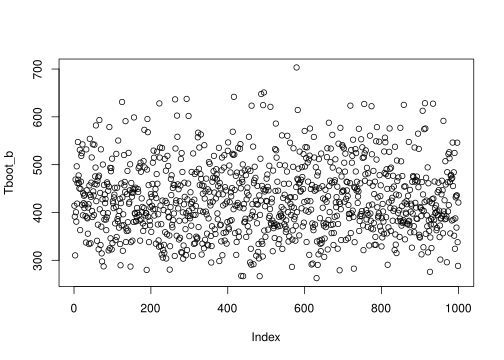
\includegraphics[width=0.7\linewidth]{Notas-Curso-Estadistica_files/figure-latex/unnamed-chunk-89-1} \end{center}

Por supuesto podemos encontrar los estadísticos usuales para esta nueva muestra

\begin{Shaded}
\begin{Highlighting}[]
\NormalTok{(Tboot <-}\StringTok{ }\KeywordTok{mean}\NormalTok{(Tboot_b))}
\end{Highlighting}
\end{Shaded}

\begin{verbatim}
## [1] 428.066
\end{verbatim}

\begin{Shaded}
\begin{Highlighting}[]
\NormalTok{(Vboot <-}\StringTok{ }\KeywordTok{var}\NormalTok{(Tboot_b))}
\end{Highlighting}
\end{Shaded}

\begin{verbatim}
## [1] 5504.701
\end{verbatim}

\begin{Shaded}
\begin{Highlighting}[]
\NormalTok{(sdboot <-}\StringTok{ }\KeywordTok{sqrt}\NormalTok{(Vboot))}
\end{Highlighting}
\end{Shaded}

\begin{verbatim}
## [1] 74.19367
\end{verbatim}

\begin{verbatim}

### Intervalos de confianza



\subsubsection{Intervalo Normal}

Este es el más sencillo y se escribe como

\begin{equation}
T_{n} \pm z_{\alpha / 2} \widehat{\mathrm{Se}}_{\mathrm{boot}}
\end{equation}

\BeginKnitrBlock{remark}<div class="remark">\iffalse{} <span class="remark"><em>Nota: </em></span>  \fi{}Este intervalo solo funciona si la distribución de \(T_{n}\) es normal.</div>\EndKnitrBlock{remark}
\BeginKnitrBlock{exercise}<div class="exercise"><span class="exercise" id="exr:unnamed-chunk-94"><strong>\label{exr:unnamed-chunk-94} </strong></span>El cálculo de este intervalo es</div>\EndKnitrBlock{exercise}
```r
c(Tn - z * sdboot, Tn + z * sdboot)
\end{verbatim}

\begin{verbatim}
## [1] 283.8315 574.6653
\end{verbatim}

\begin{verbatim}

\subsubsection{Intervalo pivotal}

Sea  \(\theta=T(F)\) y  \(\widehat{\theta}_{n}=T\left(\widehat{F}_{n}\right)\) y defina la cantidad pivotal  \(R_{n}=\widehat{\theta}_{n}-\theta .\)

Sea  \(H(r)\) la función de distribución del pivote:
\[
H(r)=\mathbb{P}_{F}\left(R_{n} \leq r\right).
\]

Además considere  \(C_{n}^{\star}=(a, b)\)  donde
\[
a=\widehat{\theta}_{n}-H^{-1}\left(1-\frac{\alpha}{2}\right) \quad \text { y } \quad b=\widehat{\theta}_{n}-H^{-1}\left(\frac{\alpha}{2}\right).
\]

Se sigue que
\begin{align*}
\mathbb{P}(a \leq \theta \leq b)
&=\mathbb{P}\left(\widehat{\theta}_{n}-b \leq R_{n} \leq \widehat{\theta}_{n}-a\right) \\
&=H\left(\widehat{\theta}_{n}-a\right)-H\left(\widehat{\theta}_{n}-b\right) \\
&=H\left(H^{-1}\left(1-\frac{\alpha}{2}\right)\right)-H\left(H^{-1}\left(\frac{\alpha}{2}\right)\right) \\
&=1-\frac{\alpha}{2}-\frac{\alpha}{2}=1-\alpha
\end{align*}
\BeginKnitrBlock{remark}<div class="remark">\iffalse{} <span class="remark"><em>Nota: </em></span>  \fi{}\(C_{n}^{\star}=(a, b)\)  es un intervalo de confianza al \(1-\alpha\) de confianza.
El problema es que este intervalo depende de \(H\) desconocido.
</div>\EndKnitrBlock{remark}


Para resolver este problema, se puede construir una versión _bootstrap_ de \(H\) usando lo que sabemos hasta ahora.

\[
\widehat{H}(r)=\frac{1}{B} \sum_{b=1}^{B} I\left(R_{n, b}^{*} \leq r\right)
\]
donde \(R_{n, b}^{*}=\widehat{\theta}_{n, b}^{*}-\widehat{\theta}_{n}\).

Sea  \(r_{\beta}^{*}\) el cuantil muestral de tamaño  \(\beta\) de  \(\left(R_{n, 1}^{*}, \ldots, R_{n, B}^{*}\right)\) y sea \(\theta_{\beta}^{*}\) el cuantil muestral de tamaño  \(\beta\) de \(\left(\theta_{n, 1}^{*}, \ldots, \theta_{n, B}^{*}\right)\).

\BeginKnitrBlock{remark}<div class="remark">\iffalse{} <span class="remark"><em>Nota: </em></span>  \fi{}Según la notación anterior note que
\begin{equation*}
r_{\beta}^{*}= \theta_{\beta}^{*}-\widehat{\theta}_{n}
\end{equation*}</div>\EndKnitrBlock{remark}



Con estas observaciones
It follows that an approximate \(1-\alpha\) confidence interval is \(C_{n}=(\widehat{a}, \widehat{b})\) where

\begin{align*}
\widehat{a}
&= \widehat{\theta}_{n}-\widehat{H}^{-1}\left(1-\frac{\alpha}{2}\right)
&= \widehat{\theta}_{n}-r_{1-\alpha / 2}^{*}
&= \widehat{\theta}_{n}-\theta_{1-\alpha / 2}^{*} + \widehat{\theta}_{n}
&=2 \widehat{\theta}_{n}-\theta_{1-\alpha / 2}^{*} \\
\widehat{b} &=\widehat{\theta}_{n}-\widehat{H}^{-1}\left(\frac{\alpha}{2}\right)
&=\widehat{\theta}_{n}-r_{\alpha / 2}^{*}
&= \widehat{\theta}_{n}-\theta_{\alpha / 2}^{*} + \widehat{\theta}_{n}
&=2 \widehat{\theta}_{n}-\theta_{\alpha / 2}^{*}
\end{align*}

\BeginKnitrBlock{remark}<div class="remark">\iffalse{} <span class="remark"><em>Nota: </em></span>  \fi{}El intervalo de confianza pivotal de tamaño \(1-\alpha\) es
\[
  C_{n}=\left(2 \widehat{\theta}_{n}-\widehat{\theta}_{((1-\alpha / 2) B)}^{*}, 2 \widehat{\theta}_{n}-\widehat{\theta}_{((\alpha / 2) B)}^{*}\right)
  \]</div>\EndKnitrBlock{remark}

\BeginKnitrBlock{exercise}<div class="exercise"><span class="exercise" id="exr:unnamed-chunk-99"><strong>\label{exr:unnamed-chunk-99} </strong></span>El intervalo anterior para un nivel de 95\% se estima de la siguiente forma</div>\EndKnitrBlock{exercise}
```r
c(2 * Tn - quantile(Tboot_b, 1 - 0.05/2), 2 * Tn - 
    quantile(Tboot_b, 0.05/2))
\end{verbatim}

\begin{verbatim}
##    97.5%     2.5% 
## 267.1250 552.9294
\end{verbatim}

\begin{verbatim}

### Intervalo pivotal studentizado

Una mejora del intervalo anterior sería normalizar los estimadores previamente

\[
Z_{n}=\frac{T_{n}-\theta}{\widehat{\mathrm{se}}_{\mathrm{boot}}}.
\]
Como \(\theta\) es desconocido, entonces la versión a estimar es
\[
Z_{n, b}^{*}=\frac{T_{n, b}^{*}-T_{n}}{\widehat{\mathrm{se}}_{b}^{*}}
\]
donde  \(\widehat{\mathrm{se}}_{b}^{*}\) es un estimador del error estándar de  \(T_{n, b}^{*}\) no de \(T_{n}\).

\BeginKnitrBlock{remark}<div class="remark">\iffalse{} <span class="remark"><em>Nota: </em></span>  \fi{}Esto requerira estimar la varianza de \(T_{n,b}^*\) para cada \(b\).</div>\EndKnitrBlock{remark}
Con esto se puede obtener  cantidades \(Z_{n, 1}^{*}, \ldots, Z_{n, B}^{*}\) que debería ser próximos a \(Z_{n}\).

Sea \(z_{\alpha}^{*}\) del \(\alpha\) cuantiĺ de \(Z_{n, 1}^{*}, \ldots, Z_{n, B}^{*},\) entonces  \(\mathbb{P}\left(Z_{n} \leq z_{\alpha}^{*}\right) \approx \alpha\).

Define el intervalo
\begin{equation*}
C_{n}=\left(T_{n}-z_{1-\alpha / 2}^{*} \widehat{\mathrm{se}}_{\mathrm{boot}}, T_{n}-z_{\alpha / 2}^{*} \widehat{\mathrm{se}}_{\mathrm{boot}}\right)
\end{equation*}

Justificado por el siguiente cálculo:


\begin{align*}
\mathbb{P}\left(\theta \in C_{n}\right) &=\mathbb{P}\left(T_{n}-z_{1-\alpha / 2}^{*} \widehat{\mathrm{Se}}_{\mathrm{boot}} \leq \theta \leq T_{n}-z_{\alpha / 2}^{*} \widehat{\mathrm{Se}}_{\mathrm{boot}}\right) \\
&=\mathbb{P}\left(z_{\alpha / 2}^{*} \leq \frac{T_{n}-\theta}{\mathrm{se}_{\mathrm{boot}}} \leq z_{1-\alpha / 2}^{*}\right) \\
&=\mathbb{P}\left(z_{\alpha / 2}^{*} \leq Z_{n} \leq z_{1-\alpha / 2}^{*}\right) \\
& \approx 1-\alpha
\end{align*}

\BeginKnitrBlock{exercise}<div class="exercise"><span class="exercise" id="exr:unnamed-chunk-102"><strong>\label{exr:unnamed-chunk-102} </strong></span>
Note que para este caso tenemos que hacer bootstrap para cada estimador bootstrap calculado.</div>\EndKnitrBlock{exercise}

```r
B <- 1000
Tboot_b <- NULL
Tboot_bm <- NULL
sdboot_b <- NULL

for (b in 1:B) {
    xb <- sample(x, size = n, replace = TRUE)
    Tboot_b[b] <- var(xb)
    for (m in 1:B) {
        xbm <- sample(xb, size = n, replace = TRUE)
        Tboot_bm[m] <- var(xbm)
    }
    sdboot_b[b] <- sd(Tboot_bm)
}

z_star <- (Tboot_b - Tn)/sdboot_b

hist(z_star)
\end{verbatim}

\begin{center}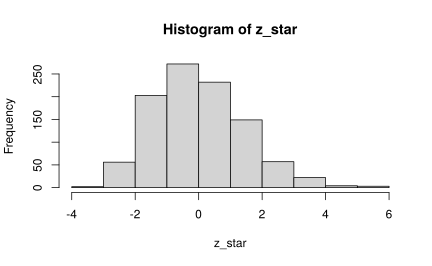
\includegraphics[width=0.7\linewidth]{Notas-Curso-Estadistica_files/figure-latex/unnamed-chunk-103-1} \end{center}

\begin{Shaded}
\begin{Highlighting}[]
\KeywordTok{c}\NormalTok{(Tn }\OperatorTok{-}\StringTok{ }\KeywordTok{quantile}\NormalTok{(z_star, }\DecValTok{1} \OperatorTok{-}\StringTok{ }\FloatTok{0.05}\OperatorTok{/}\DecValTok{2}\NormalTok{) }\OperatorTok{*}\StringTok{ }\NormalTok{sdboot, Tn }\OperatorTok{-}\StringTok{ }
\StringTok{    }\KeywordTok{quantile}\NormalTok{(z_star, }\FloatTok{0.05}\OperatorTok{/}\DecValTok{2}\NormalTok{) }\OperatorTok{*}\StringTok{ }\NormalTok{sdboot)}
\end{Highlighting}
\end{Shaded}

\begin{verbatim}
##    97.5%     2.5% 
## 317.7259 707.0044
\end{verbatim}

\begin{verbatim}


### Resumiendo


Resumiendo todos lo métodos de cálculo de intervalos obtenemos


```r
knitr::kable(data.frame(Metodo = c("Jacknife", "Bootstrap Normal", 
    "Bootstrap Pivotal", "Bootstrap Pivotal Estudentizado"), 
    Inferior = c(Tjack - z * sdjack/sqrt(n), Tn - z * 
        sdboot, 2 * Tn - quantile(Tboot_b, 1 - 0.05/2), 
        Tn - quantile(z_star, 1 - 0.05/2) * sdboot), 
    Superior = c(Tjack + z * sdjack/sqrt(n), Tn + z * 
        sdboot, 2 * Tn - quantile(Tboot_b, 0.05/2), 
        Tn - quantile(z_star, 0.05/2) * sdboot)))
\end{verbatim}

\begin{tabular}{l|r|r}
\hline
Metodo & Inferior & Superior\\
\hline
Jacknife & 285.1679 & 573.3289\\
\hline
Bootstrap Normal & 283.8315 & 574.6653\\
\hline
Bootstrap Pivotal & 271.2827 & 551.4989\\
\hline
Bootstrap Pivotal Estudentizado & 317.7259 & 707.0044\\
\hline
\end{tabular}

\hypertarget{ejercicios-1}{%
\section{Ejercicios}\label{ejercicios-1}}

\begin{enumerate}
\def\labelenumi{\arabic{enumi}.}
\item
  Repita los ejercicios anteriores para calcular intervalos de confianza para la distancia promedio y la varianza del desplazamiento de las personas. Use los métodos de Jacknife y Bootstrap (con todos sus intervalos de confianza).
  Dada que la distancia es una medida que puede ser influenciada por distancias muy cortas o muy largas, se puede calcular el logaritmo de esta variable para eliminar la escala de la distancias.
\item
  Verifique que esta última variable se podría estimar paramétricamente con una distribución normal.
  Repita los cálculos anteriores tomando como cuantiles los de una normal con media 0 y varianza 1.
\item
  Compare los intervalos calculados y comente los resultados.
\item
  Del libro \autocite{Wasserman2006} \textbf{Sección 3:} 2, 3, 7, 9, 11.
\end{enumerate}

\hypertarget{estimaciuxf3n-de-densidades-con-bayes}{%
\chapter{Estimación de densidades con Bayes}\label{estimaciuxf3n-de-densidades-con-bayes}}

\hypertarget{introducciuxf3n-a-la-estimaciuxf3n-bayesiana}{%
\section{Introducción a la estimación Bayesiana}\label{introducciuxf3n-a-la-estimaciuxf3n-bayesiana}}

\hypertarget{preliminares}{%
\subsection{Preliminares}\label{preliminares}}

Recordemos que tenemos \(f(\theta)\) la previa, \(L(\theta)\) la
verosimilitud de los datos y \(f(\theta|\text { data })\) la posterior
ajustada a los datos.

\begin{equation*}
    f(\theta | \text { data }) \propto f(\theta) L(\theta)
\end{equation*}

Además para el caso de la binomial tenemos que

\begin{equation*}
    f(y | \theta)=\theta^{\gamma}(1-\theta)^{(1-\gamma)}
\end{equation*}

y la distribución beta se escribe de la forma

\begin{align*}
    f(\theta | a, b) & =\operatorname{beta}(\theta | a, b)         \\
                     & =\theta^{(a-1)}(1-\theta)^{(b-1)} / B(a, b)
\end{align*}

donde

\begin{equation*}
    B(a, b)=\int_{0}^{1}  \theta^{(a-1)}(1-\theta)^{(b-1)}\mathrm{d} \theta.
\end{equation*}

Los valores de \(a\) y \(b\) controlan la forma de esta distribución

\begin{figure}
\centering
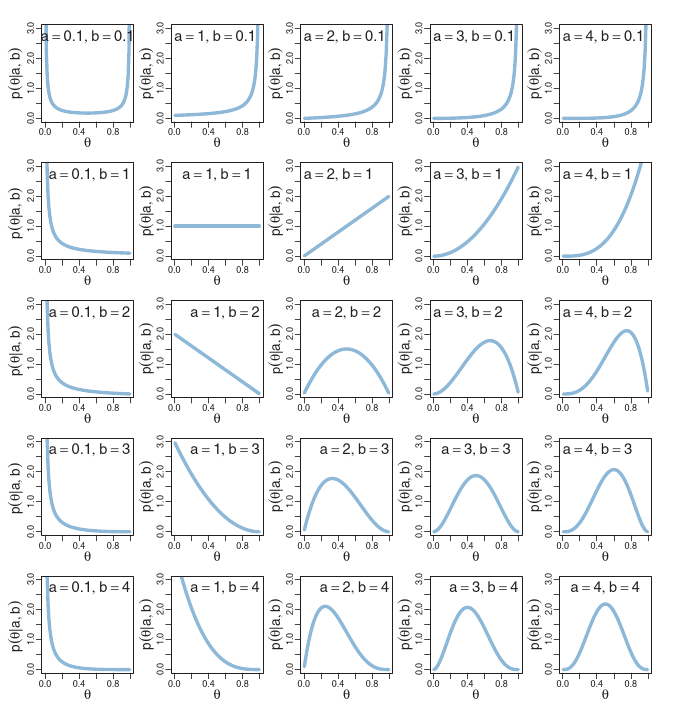
\includegraphics{manual_figures/betas.png}
\caption{Tomado de \textcite{Kruschke2014}}
\end{figure}

Una forma alternative es \(\mu=a /(a+b)\) es la media, \(\kappa=a+b\)
es la concentración y \(\omega=(a-1) /(a+b-2)\) es la moda de la
distribución Beta, entonces se cumple que

\begin{align*}
          & a=\mu \kappa \quad \text { y } \quad b=(1-\mu) \kappa                                         \\
          & a=\omega(\kappa-2)+1 \quad \text { y } \quad b=(1-\omega)(\kappa-2)+1 \text { para } \kappa>2
\end{align*}

Es decir, es posible estimar \(a\) y \(b\) de \(\kappa\), \(\mu\) y \(\omega\)

De acuerdo la combinación de estas dos distribuciones forma una familia conjugada de modo que

\begin{align*}
        f(\theta | z, N)
          & = f(z, N | \theta) f(\theta) / f(z, N)
        \quad                                              \\
          & = \theta^{z}(1-\theta)^{(N-z)} \frac{\theta^{(a-1)}(1-\theta)^{(b-1)}}{B(a, b)} / p(z, N) \\
          & = \theta^{z}(1-\theta)^{(N-z)} \theta^{(a-1)}(1-\theta)^{(b-1)} /[B(a, b) p(z, N)]        \\
          & = \theta^{((z+a)-1)}(1-\theta)^{((N-z+b)-1)} /[B(a, b) p(z, N)]                           \\
          & = \theta^{((z+a)-1)}(1-\theta)^{((N-z+b)-1)} / B(z+a, N-z+b)
\end{align*}

\hypertarget{ejemplo-sencillo}{%
\subsection{Ejemplo sencillo}\label{ejemplo-sencillo}}

Suponga que se hace una encuesta a 27 estudiantes y se encuentra que
11 dicen que duermen más de 8 horas diarias y el resto no. Nuestro
objetivo es encontrar inferencias sobre la proporción \(p\) de
estudiantes que duermen al menos 8 horas diarias. El modelo más
adecuado es

\[
        f(x \vert p) \propto p^s (1-p)^f
\]

donde \(s\) es la cantidad de estudiantes que duermen más de 8 horas y
\(f\) los que duermen menos de 8 horas.

Una primera aproximación para la previa es usar una distribución
discreta. En este caso, el investigador asigna una probabilidad a
cierta cantidad de horas de sueño, según su experiencia. Así, por
ejemplo:

\begin{Shaded}
\begin{Highlighting}[]
\NormalTok{(p <-}\StringTok{ }\KeywordTok{seq}\NormalTok{(}\FloatTok{0.05}\NormalTok{, }\FloatTok{0.95}\NormalTok{, }\DataTypeTok{by =} \FloatTok{0.1}\NormalTok{))}
\end{Highlighting}
\end{Shaded}

\begin{verbatim}
##  [1] 0.05 0.15 0.25 0.35 0.45 0.55 0.65 0.75 0.85 0.95
\end{verbatim}

\begin{Shaded}
\begin{Highlighting}[]
\NormalTok{(prior <-}\StringTok{ }\KeywordTok{c}\NormalTok{(}\DecValTok{1}\NormalTok{, }\FloatTok{5.2}\NormalTok{, }\DecValTok{8}\NormalTok{, }\FloatTok{7.2}\NormalTok{, }\FloatTok{4.6}\NormalTok{, }\FloatTok{2.1}\NormalTok{, }\FloatTok{0.7}\NormalTok{, }\FloatTok{0.1}\NormalTok{, }\DecValTok{0}\NormalTok{, }
    \DecValTok{0}\NormalTok{))}
\end{Highlighting}
\end{Shaded}

\begin{verbatim}
##  [1] 1.0 5.2 8.0 7.2 4.6 2.1 0.7 0.1 0.0 0.0
\end{verbatim}

\begin{Shaded}
\begin{Highlighting}[]
\NormalTok{(prior <-}\StringTok{ }\NormalTok{prior}\OperatorTok{/}\KeywordTok{sum}\NormalTok{(prior))}
\end{Highlighting}
\end{Shaded}

\begin{verbatim}
##  [1] 0.034602076 0.179930796 0.276816609 0.249134948 0.159169550 0.072664360
##  [7] 0.024221453 0.003460208 0.000000000 0.000000000
\end{verbatim}

\begin{Shaded}
\begin{Highlighting}[]
\KeywordTok{plot}\NormalTok{(p, prior, }\DataTypeTok{type =} \StringTok{"h"}\NormalTok{, }\DataTypeTok{ylab =} \StringTok{"Probabilidad Previa"}\NormalTok{)}
\end{Highlighting}
\end{Shaded}

\begin{center}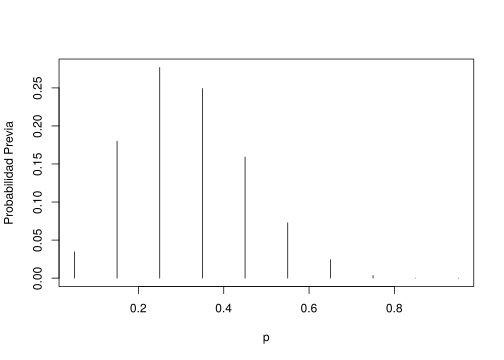
\includegraphics[width=0.7\linewidth]{Notas-Curso-Estadistica_files/figure-latex/unnamed-chunk-107-1} \end{center}

El paquete \texttt{LearnBayes} tiene la función \texttt{pdisc} que estima la
distribución posterior para una previa discreta binomial. Recuerde que
el valor 11 representa la cantidad de estudiantes con más de 8 horas
de sueño y 16 lo que no duermen esa cantidad.

\begin{Shaded}
\begin{Highlighting}[]
\KeywordTok{library}\NormalTok{(LearnBayes)}
\NormalTok{data <-}\StringTok{ }\KeywordTok{c}\NormalTok{(}\DecValTok{11}\NormalTok{, }\DecValTok{16}\NormalTok{)}
\NormalTok{post <-}\StringTok{ }\KeywordTok{pdisc}\NormalTok{(p, prior, data)}
\KeywordTok{round}\NormalTok{(}\KeywordTok{cbind}\NormalTok{(p, prior, post), }\DecValTok{2}\NormalTok{)}
\end{Highlighting}
\end{Shaded}

\begin{verbatim}
##          p prior post
##  [1,] 0.05  0.03 0.00
##  [2,] 0.15  0.18 0.00
##  [3,] 0.25  0.28 0.13
##  [4,] 0.35  0.25 0.48
##  [5,] 0.45  0.16 0.33
##  [6,] 0.55  0.07 0.06
##  [7,] 0.65  0.02 0.00
##  [8,] 0.75  0.00 0.00
##  [9,] 0.85  0.00 0.00
## [10,] 0.95  0.00 0.00
\end{verbatim}

Y podemos ver la diferencia entre la previa (negro) y la posterior
(roja),

\begin{Shaded}
\begin{Highlighting}[]
\KeywordTok{plot}\NormalTok{(p, post, }\DataTypeTok{type =} \StringTok{"h"}\NormalTok{, }\DataTypeTok{col =} \StringTok{"red"}\NormalTok{)}
\KeywordTok{lines}\NormalTok{(p }\OperatorTok{+}\StringTok{ }\FloatTok{0.01}\NormalTok{, prior, }\DataTypeTok{type =} \StringTok{"h"}\NormalTok{)}
\end{Highlighting}
\end{Shaded}

\begin{center}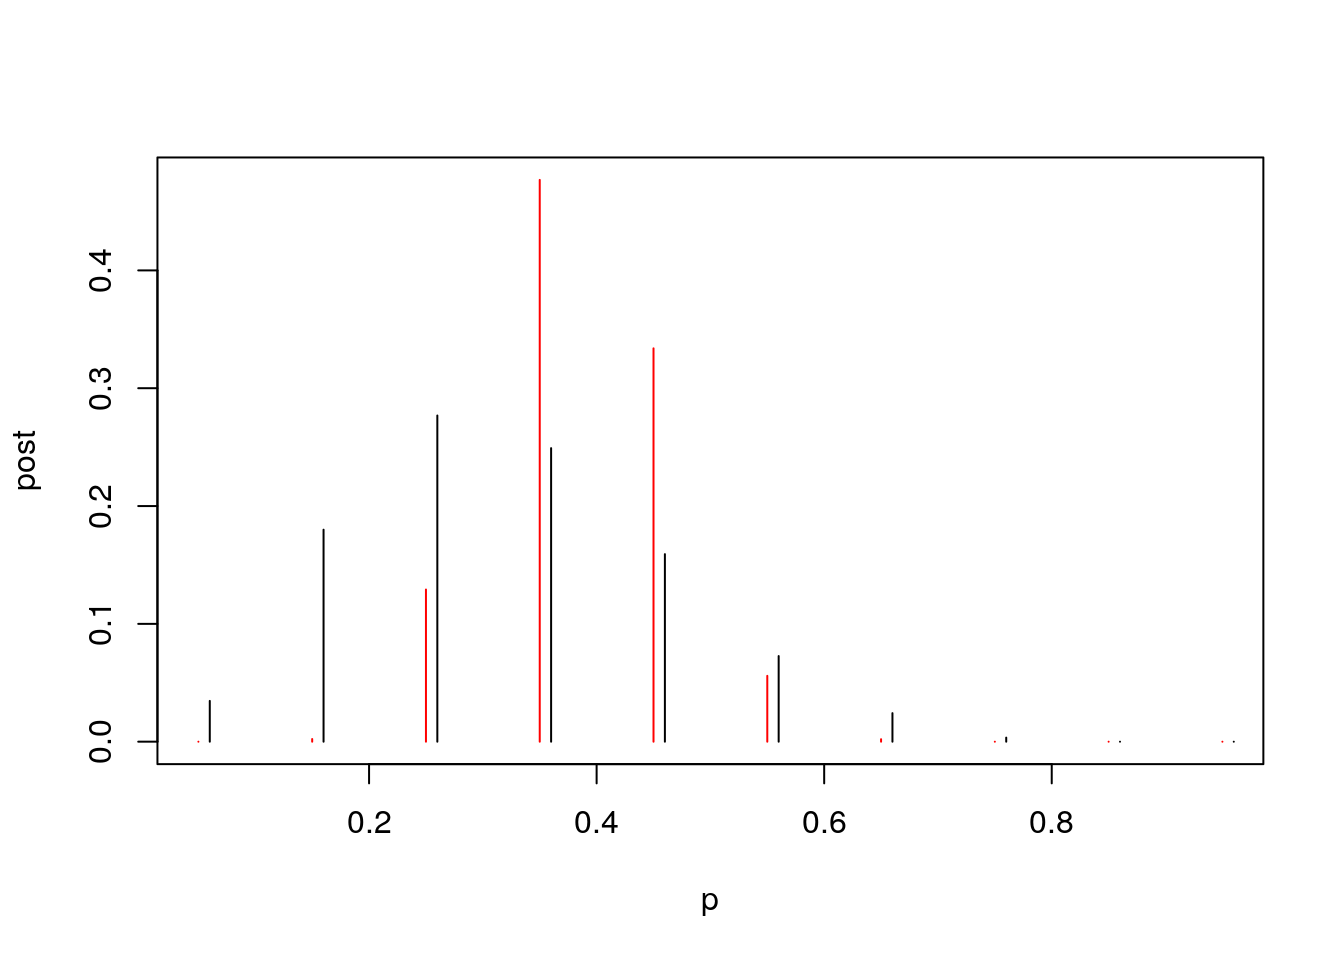
\includegraphics[width=0.7\linewidth]{Notas-Curso-Estadistica_files/figure-latex/unnamed-chunk-109-1} \end{center}

¿Qué se puede deducir de estos resultados?

\hypertarget{datos-reales}{%
\subsection{Datos reales}\label{datos-reales}}

Continuemos el ejercicio pero esta vez usando datos reales.

Carguemos los datos \texttt{studdendata} del paquete \texttt{LearnBayes}. Esta base
son preguntas que se le hicieron a un grupo de estudiantes de Bowling
Green State University. Para mayor información use \texttt{?studentdata}.

\begin{Shaded}
\begin{Highlighting}[]
\KeywordTok{data}\NormalTok{(}\StringTok{"studentdata"}\NormalTok{)}
\end{Highlighting}
\end{Shaded}

Como solo se tiene la hora de dormir y la hora de despertarse, se debe tomar la diferencia.

\begin{Shaded}
\begin{Highlighting}[]
\NormalTok{horas_sueno <-}\StringTok{ }\NormalTok{studentdata}\OperatorTok{$}\NormalTok{WakeUp }\OperatorTok{-}\StringTok{ }\NormalTok{studentdata}\OperatorTok{$}\NormalTok{ToSleep}
\NormalTok{horas_sueno <-}\StringTok{ }\KeywordTok{na.omit}\NormalTok{(horas_sueno)}
\KeywordTok{summary}\NormalTok{(horas_sueno)}
\end{Highlighting}
\end{Shaded}

\begin{verbatim}
##    Min. 1st Qu.  Median    Mean 3rd Qu.    Max. 
##   2.500   6.500   7.500   7.385   8.500  12.500
\end{verbatim}

\begin{Shaded}
\begin{Highlighting}[]
\KeywordTok{hist}\NormalTok{(horas_sueno, }\DataTypeTok{main =} \StringTok{""}\NormalTok{)}
\end{Highlighting}
\end{Shaded}

\begin{center}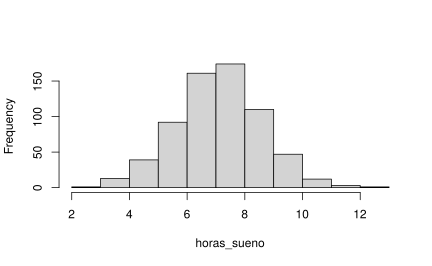
\includegraphics[width=0.7\linewidth]{Notas-Curso-Estadistica_files/figure-latex/unnamed-chunk-111-1} \end{center}

Ahora supongamos que se tiene quiere ajustar una previa continua a este modelo. Para esto usaremos una distribución Beta con parámetros \(a\) y \(b\), de la forma

\[
    f(p\vert \alpha, \beta) \propto p^{1-a} (1-p)^{1-b}.
\]

El ajuste de los parámetros de la Beta depende mucho de la información
previa que se tenga del modelo. Una forma fácil de estimarlo es a
través de cuantiles con los cuales se puede reescribir estos
parámetros. En particular, suponga que se cree que el \(50\%\) de las
observaciones la proporción será menor que 0.3 y el \(90\%\) será menor
que 0.5.

Para esto ajustaremos los siguientes parámetros

\begin{Shaded}
\begin{Highlighting}[]
\NormalTok{quantile2 <-}\StringTok{ }\KeywordTok{list}\NormalTok{(}\DataTypeTok{p =} \FloatTok{0.9}\NormalTok{, }\DataTypeTok{x =} \FloatTok{0.5}\NormalTok{)}
\NormalTok{quantile1 <-}\StringTok{ }\KeywordTok{list}\NormalTok{(}\DataTypeTok{p =} \FloatTok{0.5}\NormalTok{, }\DataTypeTok{x =} \FloatTok{0.3}\NormalTok{)}
\NormalTok{ab <-}\StringTok{ }\KeywordTok{beta.select}\NormalTok{(quantile1, quantile2)}

\NormalTok{a <-}\StringTok{ }\NormalTok{ab[}\DecValTok{1}\NormalTok{]}
\NormalTok{b <-}\StringTok{ }\NormalTok{ab[}\DecValTok{2}\NormalTok{]}
\NormalTok{s <-}\StringTok{ }\DecValTok{11}
\NormalTok{f <-}\StringTok{ }\DecValTok{16}
\end{Highlighting}
\end{Shaded}

En este caso se obtendra la distribución posterior Beta con paramétros
\(\alpha + s\) y \(\beta + f\),

\begin{Shaded}
\begin{Highlighting}[]
\KeywordTok{curve}\NormalTok{(}\KeywordTok{dbeta}\NormalTok{(x, a }\OperatorTok{+}\StringTok{ }\NormalTok{s, b }\OperatorTok{+}\StringTok{ }\NormalTok{f), }\DataTypeTok{from =} \DecValTok{0}\NormalTok{, }\DataTypeTok{to =} \DecValTok{1}\NormalTok{, }\DataTypeTok{xlab =} \StringTok{"p"}\NormalTok{, }
    \DataTypeTok{ylab =} \StringTok{"Densidad"}\NormalTok{, }\DataTypeTok{lty =} \DecValTok{1}\NormalTok{, }\DataTypeTok{lwd =} \DecValTok{4}\NormalTok{)}
\KeywordTok{curve}\NormalTok{(}\KeywordTok{dbeta}\NormalTok{(x, s }\OperatorTok{+}\StringTok{ }\DecValTok{1}\NormalTok{, f }\OperatorTok{+}\StringTok{ }\DecValTok{1}\NormalTok{), }\DataTypeTok{add =} \OtherTok{TRUE}\NormalTok{, }\DataTypeTok{lty =} \DecValTok{2}\NormalTok{, }
    \DataTypeTok{lwd =} \DecValTok{4}\NormalTok{)}
\KeywordTok{curve}\NormalTok{(}\KeywordTok{dbeta}\NormalTok{(x, a, b), }\DataTypeTok{add =} \OtherTok{TRUE}\NormalTok{, }\DataTypeTok{lty =} \DecValTok{3}\NormalTok{, }\DataTypeTok{lwd =} \DecValTok{4}\NormalTok{)}
\KeywordTok{legend}\NormalTok{(}\FloatTok{0.7}\NormalTok{, }\DecValTok{4}\NormalTok{, }\KeywordTok{c}\NormalTok{(}\StringTok{"Previa"}\NormalTok{, }\StringTok{"Verosimilitud"}\NormalTok{, }\StringTok{"Posterior"}\NormalTok{), }
    \DataTypeTok{lty =} \KeywordTok{c}\NormalTok{(}\DecValTok{3}\NormalTok{, }\DecValTok{2}\NormalTok{, }\DecValTok{1}\NormalTok{), }\DataTypeTok{lwd =} \KeywordTok{c}\NormalTok{(}\DecValTok{3}\NormalTok{, }\DecValTok{3}\NormalTok{, }\DecValTok{3}\NormalTok{))}
\end{Highlighting}
\end{Shaded}

\begin{center}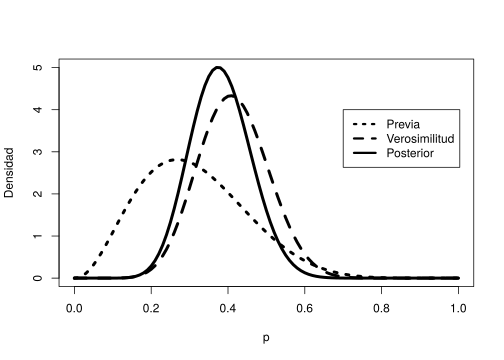
\includegraphics[width=0.7\linewidth]{Notas-Curso-Estadistica_files/figure-latex/unnamed-chunk-113-1} \end{center}

En particular, si estamos interesados en \(\mathbb{P}(p>=.5 | \text {  data })\) se puede estimar con

\begin{Shaded}
\begin{Highlighting}[]
\DecValTok{1} \OperatorTok{-}\StringTok{ }\KeywordTok{pbeta}\NormalTok{(}\FloatTok{0.5}\NormalTok{, a }\OperatorTok{+}\StringTok{ }\NormalTok{s, b }\OperatorTok{+}\StringTok{ }\NormalTok{f)}
\end{Highlighting}
\end{Shaded}

\begin{verbatim}
## [1] 0.0690226
\end{verbatim}

y el intervalo de confianza correspondiente a esta distribución sería

\begin{Shaded}
\begin{Highlighting}[]
\KeywordTok{qbeta}\NormalTok{(}\KeywordTok{c}\NormalTok{(}\FloatTok{0.05}\NormalTok{, }\FloatTok{0.95}\NormalTok{), a }\OperatorTok{+}\StringTok{ }\NormalTok{s, b }\OperatorTok{+}\StringTok{ }\NormalTok{f)}
\end{Highlighting}
\end{Shaded}

\begin{verbatim}
## [1] 0.2555267 0.5133608
\end{verbatim}

Otra opción para estimar este intervalo es simular 1000 veces la
distribución beta y observar su comportamiento en los cuantiles

\begin{Shaded}
\begin{Highlighting}[]
\NormalTok{ps <-}\StringTok{ }\KeywordTok{rbeta}\NormalTok{(}\DecValTok{1000}\NormalTok{, a }\OperatorTok{+}\StringTok{ }\NormalTok{s, b }\OperatorTok{+}\StringTok{ }\NormalTok{f)}
\KeywordTok{hist}\NormalTok{(ps, }\DataTypeTok{xlab =} \StringTok{"p"}\NormalTok{, }\DataTypeTok{main =} \StringTok{""}\NormalTok{)}
\end{Highlighting}
\end{Shaded}

\begin{center}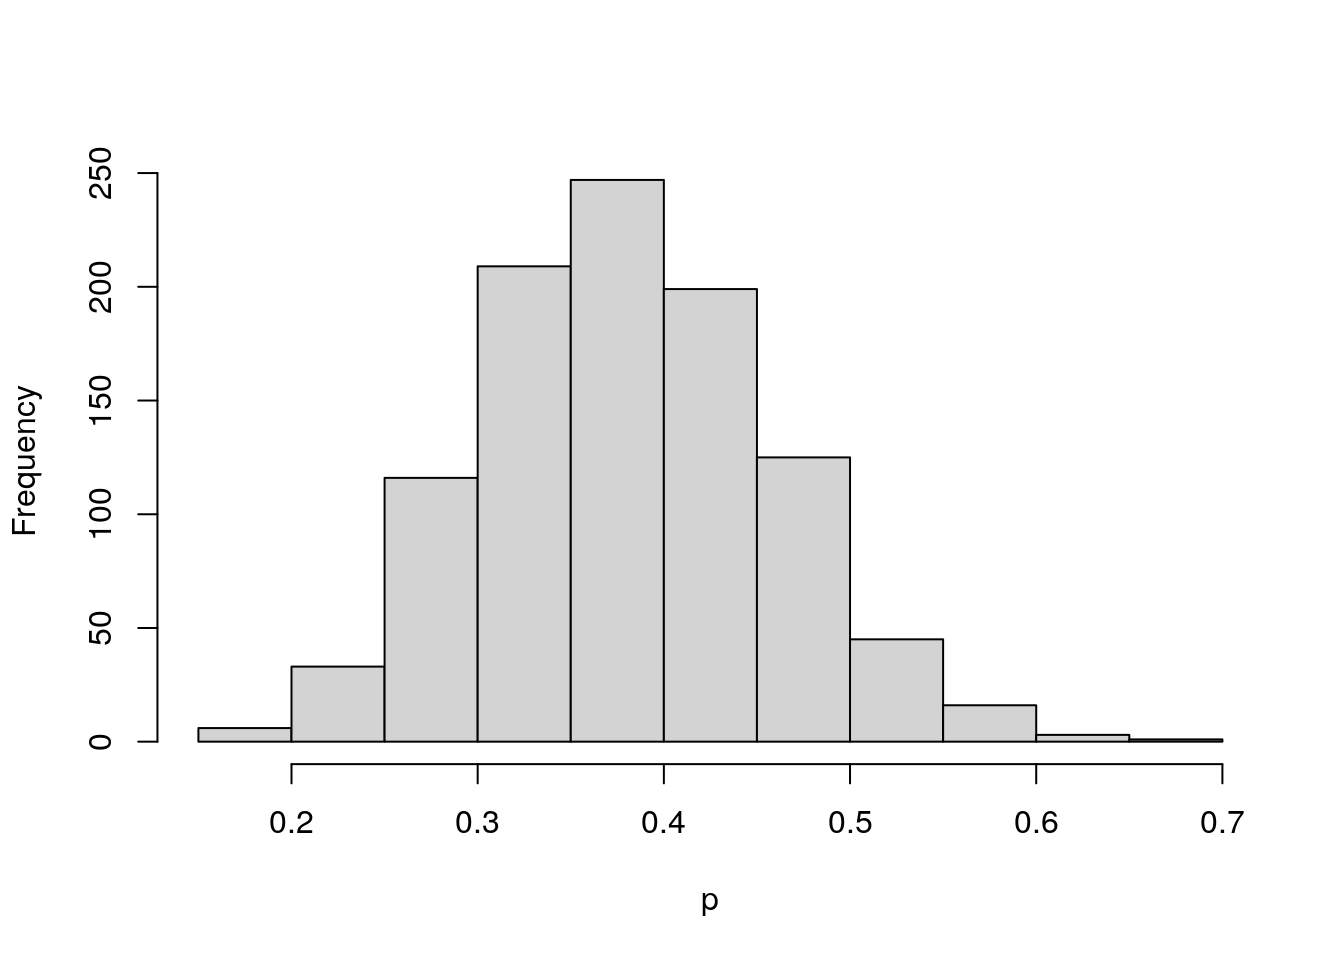
\includegraphics[width=0.7\linewidth]{Notas-Curso-Estadistica_files/figure-latex/unnamed-chunk-116-1} \end{center}

La probabilidad que este valor sea mayor que 0.5 es

\begin{Shaded}
\begin{Highlighting}[]
\KeywordTok{sum}\NormalTok{(ps }\OperatorTok{>=}\StringTok{ }\FloatTok{0.5}\NormalTok{)}\OperatorTok{/}\DecValTok{1000}
\end{Highlighting}
\end{Shaded}

\begin{verbatim}
## [1] 0.069
\end{verbatim}

\begin{Shaded}
\begin{Highlighting}[]
\KeywordTok{quantile}\NormalTok{(ps, }\KeywordTok{c}\NormalTok{(}\FloatTok{0.05}\NormalTok{, }\FloatTok{0.95}\NormalTok{))}
\end{Highlighting}
\end{Shaded}

\begin{verbatim}
##        5%       95% 
## 0.2520157 0.5196835
\end{verbatim}

\hypertarget{previa-de-histograma}{%
\section{Previa de histograma}\label{previa-de-histograma}}

El caso anterior funciona perfecto dada la combinación Binomial-Beta.

¿Qué pasaría si nuestra previa no está basada beta, sino que
quisiéramos extraerla directamente de los datos?

El método que usaremos será el siguiente:

\begin{itemize}
\tightlist
\item
  Elija una cuadrícula de valores de \(p\) sobre un intervalo que cubra
  la densidad posterior.
\item
  Calcule el producto de la probabilidad \(L (p)\) y el \(f (p)\) sobre
  esa grilla.
\item
  Normalice dividiendo cada producto por la suma de los productos. En
  esto paso, estamos aproximando la densidad posterior por una
  probabilidad discreta Distribución en la grilla.
\item
  Usando el comando \texttt{sample} de \texttt{R}, tome una muestra aleatoria con
  reemplazo de la distribución discreta.
\end{itemize}

El resultado nos debe arrojar una muestra de la distribución posterior
sobre la grilla

Suponga nuevamente que tenemos las mismas previas dadas al inicio del
capítulo

\begin{Shaded}
\begin{Highlighting}[]
\NormalTok{midpt <-}\StringTok{ }\KeywordTok{seq}\NormalTok{(}\FloatTok{0.05}\NormalTok{, }\FloatTok{0.95}\NormalTok{, }\DataTypeTok{by =} \FloatTok{0.1}\NormalTok{)}
\NormalTok{prior <-}\StringTok{ }\KeywordTok{c}\NormalTok{(}\DecValTok{1}\NormalTok{, }\FloatTok{5.2}\NormalTok{, }\DecValTok{8}\NormalTok{, }\FloatTok{7.2}\NormalTok{, }\FloatTok{4.6}\NormalTok{, }\FloatTok{2.1}\NormalTok{, }\FloatTok{0.7}\NormalTok{, }\FloatTok{0.1}\NormalTok{, }\DecValTok{0}\NormalTok{, }\DecValTok{0}\NormalTok{)}
\NormalTok{prior <-}\StringTok{ }\NormalTok{prior}\OperatorTok{/}\KeywordTok{sum}\NormalTok{(prior)}
\end{Highlighting}
\end{Shaded}

Con la función \texttt{histprior} construye los valores de \(p\) sobre una
grilla.

\begin{Shaded}
\begin{Highlighting}[]
\KeywordTok{curve}\NormalTok{(}\KeywordTok{histprior}\NormalTok{(x, midpt, prior), }\DataTypeTok{from =} \DecValTok{0}\NormalTok{, }\DataTypeTok{to =} \DecValTok{1}\NormalTok{, }
    \DataTypeTok{ylab =} \StringTok{"Densidad previa"}\NormalTok{, }\DataTypeTok{ylim =} \KeywordTok{c}\NormalTok{(}\DecValTok{0}\NormalTok{, }\FloatTok{0.3}\NormalTok{))}
\end{Highlighting}
\end{Shaded}

\begin{center}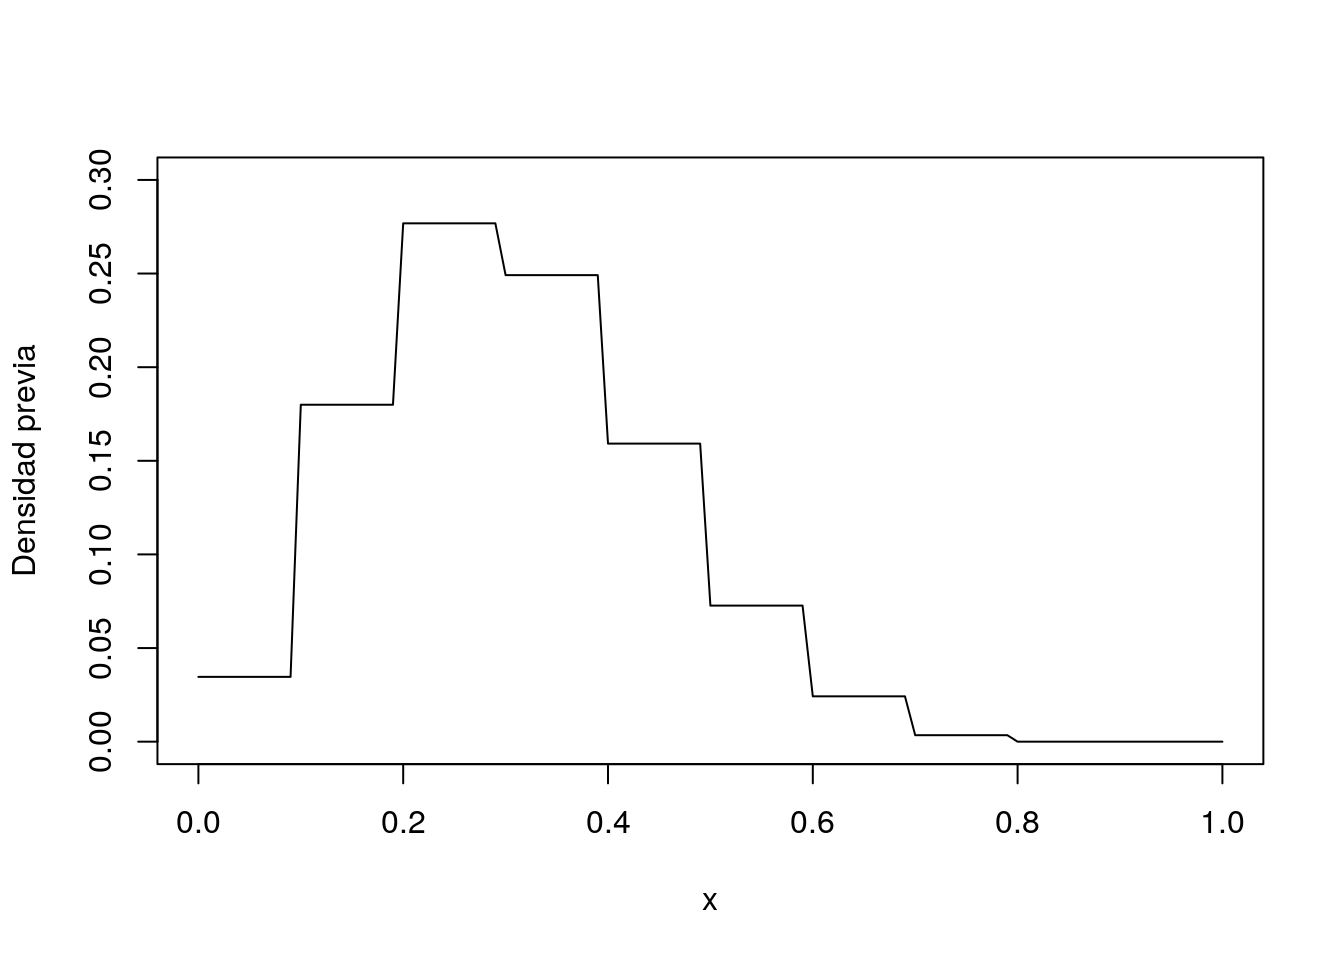
\includegraphics[width=0.7\linewidth]{Notas-Curso-Estadistica_files/figure-latex/unnamed-chunk-120-1} \end{center}

Luego recordando que nuestra posterior es \(beta(s+1,f+1)\) tenemos que

\begin{Shaded}
\begin{Highlighting}[]
\KeywordTok{curve}\NormalTok{(}\KeywordTok{histprior}\NormalTok{(x, midpt, prior) }\OperatorTok{*}\StringTok{ }\KeywordTok{dbeta}\NormalTok{(x, s }\OperatorTok{+}\StringTok{ }\DecValTok{1}\NormalTok{, }
\NormalTok{    f }\OperatorTok{+}\StringTok{ }\DecValTok{1}\NormalTok{), }\DataTypeTok{from =} \DecValTok{0}\NormalTok{, }\DataTypeTok{to =} \DecValTok{1}\NormalTok{, }\DataTypeTok{ylab =} \StringTok{"Densidad posterior"}\NormalTok{)}
\end{Highlighting}
\end{Shaded}

\begin{center}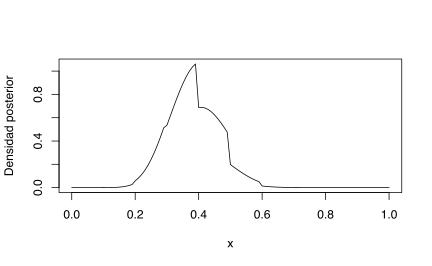
\includegraphics[width=0.7\linewidth]{Notas-Curso-Estadistica_files/figure-latex/unnamed-chunk-121-1} \end{center}

Para conseguir la distribución posterior, solo debemos de construirla para una secuencia ordenada de valores \(p\)

\begin{Shaded}
\begin{Highlighting}[]
\NormalTok{p =}\StringTok{ }\KeywordTok{seq}\NormalTok{(}\DecValTok{0}\NormalTok{, }\DecValTok{1}\NormalTok{, }\DataTypeTok{length =} \DecValTok{1000}\NormalTok{)}
\NormalTok{post =}\StringTok{ }\KeywordTok{histprior}\NormalTok{(p, midpt, prior) }\OperatorTok{*}\StringTok{ }\KeywordTok{dbeta}\NormalTok{(p, s }\OperatorTok{+}\StringTok{ }\DecValTok{1}\NormalTok{, }
\NormalTok{    f }\OperatorTok{+}\StringTok{ }\DecValTok{1}\NormalTok{)}
\NormalTok{post =}\StringTok{ }\NormalTok{post}\OperatorTok{/}\KeywordTok{sum}\NormalTok{(post)}
\end{Highlighting}
\end{Shaded}

Finalmente basta con tomar el muestreo de la posterior

\begin{Shaded}
\begin{Highlighting}[]
\NormalTok{ps <-}\StringTok{ }\KeywordTok{sample}\NormalTok{(p, }\DataTypeTok{replace =} \OtherTok{TRUE}\NormalTok{, }\DataTypeTok{prob =}\NormalTok{ post)}
\KeywordTok{hist}\NormalTok{(ps, }\DataTypeTok{xlab =} \StringTok{"p"}\NormalTok{, }\DataTypeTok{main =} \StringTok{""}\NormalTok{)}
\end{Highlighting}
\end{Shaded}

\begin{center}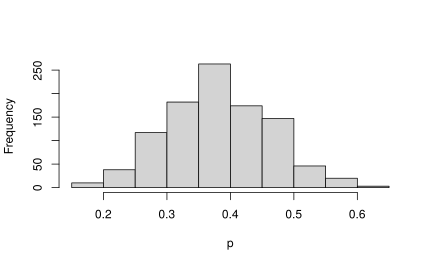
\includegraphics[width=0.7\linewidth]{Notas-Curso-Estadistica_files/figure-latex/unnamed-chunk-123-1} \end{center}

\hypertarget{muxe9todos-monte-carlo}{%
\section{Métodos Monte Carlo}\label{muxe9todos-monte-carlo}}

\hypertarget{una-moneda}{%
\section{Una moneda}\label{una-moneda}}

El tratamiento clásico de la estimación de parámetros bayesiana nos dice que si tenemos una densidad previa y la ``combinamos'' con la verosimilitud de los datos, estos nos dará una densidad con más información. Se podría repetir el proceso varias veces para tratar de ajustar mejor la densidad posterior.

Sin embargo, se podría usar potencia de los métodos Monte Carlo para que esta búsqueda sea muy efectiva para encontrar los parámetros adecuados.

\hypertarget{ejemplo-del-viajero}{%
\subsection{Ejemplo del viajero}\label{ejemplo-del-viajero}}

Suponga que tenemos un viajero que quiere estar en 7 lugares distintos (suponga que están en línea recta) y la probabilidad de pasar a un lugar a otro se decide tirando una moneda no sesgada (50\% a la derecha y 50\% a la izquierda).

Este caso sería una simple caminata aleatoria sin ningún interés en particular.

Suponga además, que el viajero quiere estar más tiempo donde haya una mayor cantidad de personas \(P\) pero siguiendo ese patrón aleatorio. Entonces la forma de describir su decisión de moverse sería:

\begin{itemize}
\tightlist
\item
  Tira la moneda y decide si va a la izquierda o la derecha.

  \begin{enumerate}
  \def\labelenumi{\arabic{enumi}.}
  \item
    Si el lugar nuevo tiene \textbf{MÁS} personas que el actual salta a ese lugar.
  \item
    Si el lugar nuevo tiene \textbf{MENOS} personas entonces el viajero tiene que decidir si se queda o se mueve. \textbar{} calcula la probabilidad de moverse como \(p_{moverse} = P_{nuevo}/P_{actual}\).

    \textbf{Tira un número aleatorio entre 0 y 1 \(r\)}

    \begin{enumerate}
    \def\labelenumii{\arabic{enumii}.}
    \tightlist
    \item
      Si \(p_{moverse}>r\) entonces se mueve.
    \item
      Sino, se queda donde está.
    \end{enumerate}
  \end{enumerate}
\end{itemize}

\begin{Shaded}
\begin{Highlighting}[]
\NormalTok{P <-}\StringTok{ }\DecValTok{1}\OperatorTok{:}\DecValTok{7}

\NormalTok{pos_actual <-}\StringTok{ }\KeywordTok{sample}\NormalTok{(P, }\DecValTok{1}\NormalTok{)}
\NormalTok{pos_nueva <-}\StringTok{ }\NormalTok{pos_actual}

\NormalTok{n_pasos <-}\StringTok{ }\DecValTok{50000}
\NormalTok{trayectoria <-}\StringTok{ }\KeywordTok{numeric}\NormalTok{(n_pasos)}

\NormalTok{trayectoria[}\DecValTok{1}\NormalTok{] <-}\StringTok{ }\NormalTok{pos_actual}

\ControlFlowTok{for}\NormalTok{ (k }\ControlFlowTok{in} \DecValTok{2}\OperatorTok{:}\NormalTok{n_pasos) \{}
    \CommentTok{# Tira la moneda para decidir}
    
\NormalTok{    moneda <-}\StringTok{ }\KeywordTok{rbinom}\NormalTok{(}\DecValTok{1}\NormalTok{, }\DecValTok{1}\NormalTok{, }\FloatTok{0.5}\NormalTok{)}
    \CommentTok{# moneda es 0 o 1}
\NormalTok{    pos_nueva <-}\StringTok{ }\NormalTok{pos_actual}
    \ControlFlowTok{if}\NormalTok{ (moneda }\OperatorTok{==}\StringTok{ }\DecValTok{1} \OperatorTok{&}\StringTok{ }\NormalTok{(pos_actual }\OperatorTok{+}\StringTok{ }\DecValTok{1}\NormalTok{) }\OperatorTok{<=}\StringTok{ }\DecValTok{7}\NormalTok{) \{}
\NormalTok{        pos_nueva =}\StringTok{ }\NormalTok{pos_actual }\OperatorTok{+}\StringTok{ }\DecValTok{1}
\NormalTok{    \} }\ControlFlowTok{else} \ControlFlowTok{if}\NormalTok{ (moneda }\OperatorTok{==}\StringTok{ }\DecValTok{0} \OperatorTok{&}\StringTok{ }\NormalTok{(pos_actual }\OperatorTok{-}\StringTok{ }\DecValTok{1}\NormalTok{) }\OperatorTok{>=}\StringTok{ }\DecValTok{1}\NormalTok{) \{}
\NormalTok{        pos_nueva <-}\StringTok{ }\NormalTok{pos_actual }\OperatorTok{-}\StringTok{ }\DecValTok{1}
\NormalTok{    \}}
    
\NormalTok{    p_moverse <-}\StringTok{ }\KeywordTok{min}\NormalTok{(pos_nueva}\OperatorTok{/}\NormalTok{pos_actual, }\DecValTok{1}\NormalTok{)}
    
\NormalTok{    hay_movimiento <-}\StringTok{ }\DecValTok{1} \OperatorTok{-}\StringTok{ }\NormalTok{p_moverse }\OperatorTok{<=}\StringTok{ }\KeywordTok{runif}\NormalTok{(}\DecValTok{1}\NormalTok{)}
    
    \ControlFlowTok{if}\NormalTok{ (hay_movimiento) \{}
\NormalTok{        pos_actual <-}\StringTok{ }\NormalTok{pos_nueva}
\NormalTok{    \}}
    
\NormalTok{    trayectoria[k] <-}\StringTok{ }\NormalTok{pos_nueva}
\NormalTok{\}}
\end{Highlighting}
\end{Shaded}

\begin{Shaded}
\begin{Highlighting}[]
\NormalTok{df <-}\StringTok{ }\KeywordTok{data.frame}\NormalTok{(}\DataTypeTok{x =} \DecValTok{1}\OperatorTok{:}\NormalTok{n_pasos, }\DataTypeTok{P =}\NormalTok{ trayectoria)}

\KeywordTok{ggplot}\NormalTok{(df[}\DecValTok{1}\OperatorTok{:}\DecValTok{200}\NormalTok{, ]) }\OperatorTok{+}\StringTok{ }\KeywordTok{geom_line}\NormalTok{(}\KeywordTok{aes}\NormalTok{(x, P)) }\OperatorTok{+}\StringTok{ }\KeywordTok{coord_flip}\NormalTok{() }\OperatorTok{+}\StringTok{ }
\StringTok{    }\KeywordTok{theme_minimal}\NormalTok{(}\DataTypeTok{base_size =} \DecValTok{16}\NormalTok{)}
\end{Highlighting}
\end{Shaded}

\begin{center}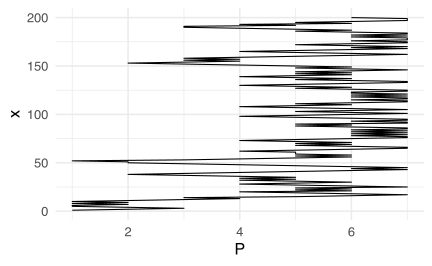
\includegraphics[width=0.7\linewidth]{Notas-Curso-Estadistica_files/figure-latex/unnamed-chunk-125-1} \end{center}

\begin{Shaded}
\begin{Highlighting}[]
\KeywordTok{ggplot}\NormalTok{(df) }\OperatorTok{+}\StringTok{ }\KeywordTok{geom_histogram}\NormalTok{(}\KeywordTok{aes}\NormalTok{(P), }\DataTypeTok{stat =} \StringTok{"count"}\NormalTok{) }\OperatorTok{+}\StringTok{ }
\StringTok{    }\KeywordTok{theme_minimal}\NormalTok{(}\DataTypeTok{base_size =} \DecValTok{16}\NormalTok{)}
\end{Highlighting}
\end{Shaded}

\begin{center}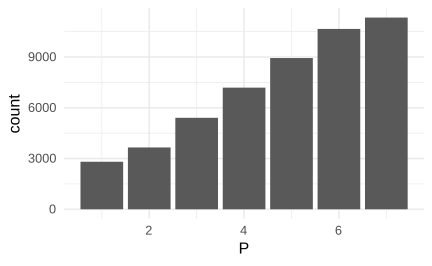
\includegraphics[width=0.7\linewidth]{Notas-Curso-Estadistica_files/figure-latex/unnamed-chunk-125-2} \end{center}

\begin{Shaded}
\begin{Highlighting}[]
\KeywordTok{mean}\NormalTok{(trayectoria)}
\end{Highlighting}
\end{Shaded}

\begin{verbatim}
## [1] 4.86008
\end{verbatim}

\begin{Shaded}
\begin{Highlighting}[]
\KeywordTok{sd}\NormalTok{(trayectoria)}
\end{Highlighting}
\end{Shaded}

\begin{verbatim}
## [1] 1.798412
\end{verbatim}

\hypertarget{cadenas-de-markov}{%
\subsection{Cadenas de Markov}\label{cadenas-de-markov}}

Recuerde que estamos buscando el \enquote{camino} que el viajero tomará para pasar la mayor parte del tiempo de en los lugares más poblados (con mayor \(\theta\)).

\begin{equation*}
\theta_{1} \curvearrowright \theta_{2} \curvearrowright \ldots \curvearrowright \theta_{50000}.
\end{equation*}

Denotamos \(\theta_{1}\to\theta_{2}\) si el viajero pasó de \(\theta_{1}\) hacia \(\theta_{2}\).

Entonces

\begin{itemize}
\tightlist
\item
  \(\mathbb{P}\left(\theta \rightarrow \theta+1\right)=0.5 \min \left(\frac{P(\theta+1)}{P(\theta)} / , 1\right)\)
\item
  \(\mathbb{P}\left(\theta + 1 \rightarrow \theta\right)=0.5 \min \left(\frac{P(\theta)}{P(\theta+1)} / , 1\right)\)
\end{itemize}

Entonces la razón entre estas dos probabilidades es

\begin{align*}
    \frac{\mathbb{P}\left(\theta \rightarrow \theta+1\right)}{\mathbb{P}\left(\theta +1 \rightarrow \theta\right)}
      & =\frac{0.5 \min (P(\theta+1) / P(\theta), 1)}{0.5 \min (P(\theta) / P(\theta+1), 1)} \\
      & =\left\{\begin{array}{ll}
        \frac{P(\theta+1)}{P(\theta) }
          & \text { si } P(\theta+1)>P(\theta) \\
        \frac{P(\theta+1) }{P(\theta)}
          & \text { si } P(\theta+1)<P(\theta)
    \end{array}\right.                                             \\
    \, & =\frac{P(\theta+1)}{P(\theta)}.
\end{align*}

Es decir que la razón de las probabilidades es equivalente a la razón entre las proporción de las poblaciones. Por lo tanto la mayoría de las veces se estará en los lugares con mayor población.

Esta cadena se puede escribir usando una matriz de transición de la forma

\begin{equation*}
T= \left(\begin{array}{ccccc}
\ddots & \mathbb{P}(\theta-2 \rightarrow \theta-1) & 0 & 0 & 0 \\
\ddots & \mathbb{P}(\theta-1 \rightarrow \theta-1) & \mathbb{P}(\theta-1 \rightarrow \theta) & 0 & 0 \\
0 & \mathbb{P}(\theta \rightarrow \theta-1) & \mathbb{P}(\theta \rightarrow \theta) & \mathbb{P}(\theta \rightarrow \theta+1) & 0 \\
0 & 0 & \mathbb{P}(\theta+1 \rightarrow \theta) & \mathbb{P}(\theta+1 \rightarrow \theta+1) & \ddots \\
0 & 0 & 0 & \mathbb{P}(\theta+2 \rightarrow \theta+1) & \ddots
\end{array}\right)
\end{equation*}

La matriz \(T\) tiene las propiedades

\begin{enumerate}
\def\labelenumi{\arabic{enumi}.}
\tightlist
\item
  Existencia de una única distribución estacionaria (llamada \(f\) más adelante).
\item
  Es ergódica, i.e., es aperíodica y positiva recurrente. Recuerde que una cadena de markov es érgodica si siempre se puede pasar de un estado a otro (no necesariamente en 1 paso). Otra forma de verlo es que la para alguna potencia de \(T\) todos los sus elementos serán positivos estrictos.
\end{enumerate}

\hypertarget{el-algoritmo-de-metropolis-hasting}{%
\subsection{El algoritmo de Metropolis-Hasting}\label{el-algoritmo-de-metropolis-hasting}}

El ejemplo anterior era bastante sencillo pero demuestra que se puede
encontrar el mejor estimador posible simplemente ejecutando una y otra
vez maximizando la estadía en los lugares más poblados.

En este ejemplo la función a maximizar es la cantidad de personas
\(P(\theta)=\theta\), pero en general nuestro objetivo será maximizar
la distribución posterior \(f(\theta| \text{ datos })\).

En palabras simples el algoritmo de Metropoli Hasting es

\begin{enumerate}
\def\labelenumi{\arabic{enumi}.}
\tightlist
\item
  Simule un valor \(\theta^{*}\) de una densidad de propuesta
  \(p\left(\theta^{*} | \theta^{t-1}\right)\)
\item
  Estime la razón
  \[
   R=\frac{f\left(\theta^{*}\right) L\left(\theta^{t-1} |
       \theta^{*}\right)}{f\left(\theta^{t-1}\right) L\left(\theta^{*} |
       \theta^{t-1}\right)}
  \]
\item
  Estima la probabilidad de aceptación \(p_{\text {moverse }}=\min \{R, 1\}\).
\item
  Tome \(\theta^{t}\) tal que \(\theta^{t}=\theta^{*}\)
  con probabilidad \(p_{\text {moverse }}\); en otro caso \(\theta^{t}=\) \(\theta^{t-1}\)
\end{enumerate}

El algoritmo de Metropolis-Hastings se puede construir de muchas
formas, dependiendo de la densidad de proposición

Si esta es independiente de las elecciones anteriores entonces,
\[
    L\left(\theta^{*} | \theta^{t-1}\right)=L\left(\theta^{*}\right)
\]

Otras formas es escoger
\[
    L\left(\theta^{*} |
    \theta^{t-1}\right)=h\left(\theta^{*}-\theta^{t-1}\right)
\]
donde \(h\) es simétrica alrededor del origen. En este tipo de
cadenas, la razón \(R\) tiene la forma
\[
    R=\frac{f\left(\theta^{*}\right)}{f\left(\theta^{t-1}\right)}
\]

Una última opción es tomar
\[
    \theta^{*}=\theta^{t-1}+ Z
\]

donde \(Z\) es una normal centrada con cierta estructura de varianza.

\hypertarget{por-quuxe9-el-algoritmo-de-metropolis-hasting-funciona}{%
\subsection{¿Por qué el algoritmo de Metropolis Hasting funciona?}\label{por-quuxe9-el-algoritmo-de-metropolis-hasting-funciona}}

\begin{equation}
\mathbb{P}\left(\theta_{\star} | \theta^{(t)}\right)=L\left(\theta_{\star} | \theta^{(t)}\right) \cdot \min \left\{1, \frac{f\left(\theta_{\star}\right) L\left(\theta^{(t)} | \theta_{\star}\right)}{f\left(\theta^{(t)}\right) L\left(\theta_{\star} | \theta^{(t)}\right)}\right\}
\end{equation}

Si se comienza en \(f\left(\theta^{(t)}\right)\) entonces

\begin{align}
\begin{array}{l}
f\left(\theta^{(t)}\right) \mathbb{P}\left(\theta_{\star} | \theta^{(t)}\right) \\
\quad=\quad f\left(\theta^{(t)}\right) L\left(\theta_{\star} | \theta^{(t)}\right) \min \left\{1, \frac{f\left(\theta_{\star}\right) L\left(\theta^{(t)} | \theta_{\star}\right)}{f\left(\theta^{(t)}\right) L\left(\theta_{\star} | \theta^{(t)}\right)}\right\} \\
\quad=\min \left\{f\left(\theta^{(t)}\right) L\left(\theta_{\star} | \theta^{(t)}\right), f\left(\theta_{\star}\right) L\left(\theta^{(t)} | \theta_{\star}\right)\right\} \\
\quad=\quad f\left(\theta_{\star}\right) L\left(\theta^{(t)} | \theta_{\star}\right) \min \left\{\frac{f\left(\theta^{(t)}\right) L\left(\theta_{\star} | \theta^{(t)}\right)}{f\left(\theta_{\star}\right) L\left(\theta^{\left(t | \theta_{\star}\right)}\right.}, 1\right\} \\
\quad=f\left(\theta_{\star}\right) \mathbb{P}\left(\theta^{(t)} | \theta_{\star}\right)
\end{array}
\end{align}

Asumiendo que existe una cantidad finita de estados \(\theta_{1}, \ldots, \theta_{M}\), entonces.

\begin{equation*}
f\left(\theta_{j}\right) = \underbrace{\sum_{i=1}^{M} f\left(\theta_{i}\right) \mathbb{P} \left(\theta_{j} | \theta_{i}\right)}_{\text {Probabilidad total  }}=\sum_{i=1}^{M} f\left(\theta_{j}\right) \mathbb{P} \left(\theta_{i} | \theta_{j}\right)
\end{equation*}

\begin{equation}
f(\boldsymbol{\theta})^\top T =   f(\boldsymbol{\theta})
\end{equation}

Cual indica que no importa donde empecemos siempre llegaremos a la densidad estacionaria \(f\).

\url{https://www.ece.iastate.edu/~namrata/EE527_Spring08/l4c.pdf\#page=32}

\hypertarget{extensiuxf3n-al-caso-del-viajero}{%
\subsection{Extensión al caso del viajero}\label{extensiuxf3n-al-caso-del-viajero}}

Retomemos el ejemplo del viajero. Supongamos que ahora existen una
cantidad infinita de lugares a los que puede ir y que la población de
cada isla es proporcional a la densidad posterior. Además, el viajero
podría saltar a cualquier isla que quisiera y su probabilidad de
salto cae de forma continua en el intervalo \([0,1]\).

Para hacer este ejemplo concreto, el viajero no conoce cuál es su
probabilidad de salto \(\theta\) pero sabe que ha tirado la
moneda \(N\) veces y observado \(z\) exitos. Por lo tanto tendremos
una verosimilitud de \(L(z, N | \theta)=\theta^{z}(1-\theta)^{(N-z)}\).

La previa será dada por \(f(\theta)=\operatorname{beta}(\theta | a, b)\).

Los saltos serán gobernados por una normal centrada con media
\(\sigma\) de modo que \(\Delta \theta \sim \mathcal{N}\left(0,\sigma^{2}\right)\).

Entonces el algoritmo de Metropolis Hasting se puede reformular como

\begin{enumerate}
\def\labelenumi{\arabic{enumi}.}
\item
  Simule un valor de salto\(\Delta \theta \sim \mathcal{N}\left(0,\sigma^{2}\right)\) y denote \(\theta^{t} = \theta^{t} + \Delta\theta\).
\item
  Probabilidad de aceptación \(p_{\text {moverse }}\)
  \begin{align*}
   p_{\text {moverse }}
     & =\min \left(1, \frac{P\left(\theta_{\ast}\right)}{P\left(\theta_{t-1}\right)}\right) \\
                 & =\min \left(1, \frac{p\left(D |
       \theta_{\ast}\right) p\left(\theta_{\ast}\right)}{p\left(D | \theta_{t-1}\right)
       p\left(\theta_{t-1}\right)}\right) \\
     & =\min \left(1, \frac{\operatorname{Bernoulli}\left(z, N |
       \theta_{\ast}\right)
       \operatorname{beta}\left(\theta_{\ast} | a,
       b\right)}{\operatorname{Bernoulli}\left(z, N |
       \theta_{t-1}\right)
       \operatorname{beta}\left(\theta_{t-1} | a, b\right)}\right) \\
     & =\min \left(1,
   \frac{\theta_{\ast}^{z}\left(1-\theta_{\ast}\right)^{(N-z)}
           \theta_{\ast} \left(1-\theta_{\ast}\right)^{(b-1)}
           / B(a,b)}{\theta_{t-1}^{z}\left(1-\theta_{t-1}\right)^{(N-z)}
           \theta_{t-1}^{(a-1)}\left(1-\theta_{t-1}\right)^{(b-1)}
           / B(a, b)}\right)
  \end{align*}
\item
  Tome \(\theta_{t}\) tal que \(\theta_{t}=\theta_{*}\)
  con probabilidad \(p_{\text {moverse }} ;\) en otro caso \(\theta_{t}=\) \(\theta_{t-1}\)
\end{enumerate}

En el ejemplo del viajero queremos ver la probabilidad \(\theta\) de
que salte al siguiente destino. Tomemos \(\sigma=0.2\) y supongamos
que se ha visto que el viajero de \(N=20\) y \(z=14\) éxitos. Por
cuestiones de practicidad se tomará \(\theta_0 = 0.1\).

\begin{Shaded}
\begin{Highlighting}[]
\CommentTok{# Carga de datos observados}
\NormalTok{datos_observados <-}\StringTok{ }\KeywordTok{c}\NormalTok{(}\KeywordTok{rep}\NormalTok{(}\DecValTok{0}\NormalTok{, }\DecValTok{6}\NormalTok{), }\KeywordTok{rep}\NormalTok{(}\DecValTok{1}\NormalTok{, }\DecValTok{14}\NormalTok{))}

\CommentTok{# Función de verosimilitud Binomial}
\NormalTok{verosimilitud <-}\StringTok{ }\ControlFlowTok{function}\NormalTok{(theta, data) \{}
\NormalTok{    z <-}\StringTok{ }\KeywordTok{sum}\NormalTok{(data)}
\NormalTok{    N <-}\StringTok{ }\KeywordTok{length}\NormalTok{(data)}
\NormalTok{    pDatosDadoTheta <-}\StringTok{ }\NormalTok{theta}\OperatorTok{^}\NormalTok{z }\OperatorTok{*}\StringTok{ }\NormalTok{(}\DecValTok{1} \OperatorTok{-}\StringTok{ }\NormalTok{theta)}\OperatorTok{^}\NormalTok{(N }\OperatorTok{-}\StringTok{ }\NormalTok{z)}
    \CommentTok{# Es para asegurarse que los datos caigan en [0,1].}
\NormalTok{    pDatosDadoTheta[theta }\OperatorTok{>}\StringTok{ }\DecValTok{1} \OperatorTok{|}\StringTok{ }\NormalTok{theta }\OperatorTok{<}\StringTok{ }\DecValTok{0}\NormalTok{] <-}\StringTok{ }\DecValTok{0}
    \KeywordTok{return}\NormalTok{(pDatosDadoTheta)}
\NormalTok{\}}

\CommentTok{# densidad previa}
\NormalTok{previa <-}\StringTok{ }\ControlFlowTok{function}\NormalTok{(theta) \{}
\NormalTok{    pTheta <-}\StringTok{ }\KeywordTok{dbeta}\NormalTok{(theta, }\DecValTok{1}\NormalTok{, }\DecValTok{1}\NormalTok{)}
    \CommentTok{# Es para asegurarse que los datos caigan en [0,1].}
\NormalTok{    pTheta[theta }\OperatorTok{>}\StringTok{ }\DecValTok{1} \OperatorTok{|}\StringTok{ }\NormalTok{theta }\OperatorTok{<}\StringTok{ }\DecValTok{0}\NormalTok{] <-}\StringTok{ }\DecValTok{0}
    \KeywordTok{return}\NormalTok{(pTheta)}
\NormalTok{\}}

\CommentTok{# densidad posterior}
\NormalTok{posterior <-}\StringTok{ }\ControlFlowTok{function}\NormalTok{(theta, data) \{}
\NormalTok{    posterior <-}\StringTok{ }\KeywordTok{verosimilitud}\NormalTok{(theta, data) }\OperatorTok{*}\StringTok{ }\KeywordTok{previa}\NormalTok{(theta)}
    \KeywordTok{return}\NormalTok{(posterior)}
\NormalTok{\}}

\NormalTok{n_pasos <-}\StringTok{ }\DecValTok{50000}

\NormalTok{trayectoria <-}\StringTok{ }\KeywordTok{rep}\NormalTok{(}\DecValTok{0}\NormalTok{, n_pasos)}

\CommentTok{# Valor inicial}
\NormalTok{trayectoria[}\DecValTok{1}\NormalTok{] <-}\StringTok{ }\FloatTok{0.01}

\NormalTok{n_aceptados <-}\StringTok{ }\DecValTok{0}
\NormalTok{n_rechazados <-}\StringTok{ }\DecValTok{0}


\NormalTok{sigma <-}\StringTok{ }\FloatTok{0.2}

\ControlFlowTok{for}\NormalTok{ (t }\ControlFlowTok{in} \DecValTok{2}\OperatorTok{:}\NormalTok{(n_pasos }\OperatorTok{-}\StringTok{ }\DecValTok{1}\NormalTok{)) \{}
\NormalTok{    pos_actual <-}\StringTok{ }\NormalTok{trayectoria[t]}
    
\NormalTok{    salto_propuesto <-}\StringTok{ }\KeywordTok{rnorm}\NormalTok{(}\DecValTok{1}\NormalTok{, }\DataTypeTok{mean =} \DecValTok{0}\NormalTok{, }\DataTypeTok{sd =}\NormalTok{ sigma)}
    
\NormalTok{    proba_aceptacion <-}\StringTok{ }\KeywordTok{min}\NormalTok{(}\DecValTok{1}\NormalTok{, }\KeywordTok{posterior}\NormalTok{(pos_actual }\OperatorTok{+}\StringTok{ }
\StringTok{        }\NormalTok{salto_propuesto, datos_observados)}\OperatorTok{/}\KeywordTok{posterior}\NormalTok{(pos_actual, }
\NormalTok{        datos_observados))}
    
    \CommentTok{# Aceptamos el salto?}
    \ControlFlowTok{if}\NormalTok{ (}\KeywordTok{runif}\NormalTok{(}\DecValTok{1}\NormalTok{) }\OperatorTok{<}\StringTok{ }\NormalTok{proba_aceptacion) \{}
        \CommentTok{# Aceptados}
\NormalTok{        trayectoria[t }\OperatorTok{+}\StringTok{ }\DecValTok{1}\NormalTok{] <-}\StringTok{ }\NormalTok{pos_actual }\OperatorTok{+}\StringTok{ }\NormalTok{salto_propuesto}
\NormalTok{        n_aceptados <-}\StringTok{ }\NormalTok{n_aceptados }\OperatorTok{+}\StringTok{ }\DecValTok{1}
\NormalTok{    \} }\ControlFlowTok{else}\NormalTok{ \{}
        \CommentTok{# Rechazos}
\NormalTok{        trayectoria[t }\OperatorTok{+}\StringTok{ }\DecValTok{1}\NormalTok{] <-}\StringTok{ }\NormalTok{pos_actual}
\NormalTok{        n_rechazados <-}\StringTok{ }\NormalTok{n_rechazados }\OperatorTok{+}\StringTok{ }\DecValTok{1}
\NormalTok{    \}}
\NormalTok{\}}
\end{Highlighting}
\end{Shaded}

Obtenemos una tasa de aceptación del 49.4 y tasa de rechazo del 50.59

Podemos desechar los primeros 500 pasos (por ejemplo) del proceso ya que estos son de \enquote{calentamiento}. De esta forma podremos estimar la media y la varianza de las trayectoria.

\begin{Shaded}
\begin{Highlighting}[]
\KeywordTok{mean}\NormalTok{(trayectoria[}\DecValTok{500}\OperatorTok{:}\NormalTok{n_pasos])}
\end{Highlighting}
\end{Shaded}

\begin{verbatim}
## [1] 0.6808914
\end{verbatim}

\begin{Shaded}
\begin{Highlighting}[]
\KeywordTok{sd}\NormalTok{(trayectoria[}\DecValTok{500}\OperatorTok{:}\NormalTok{n_pasos])}
\end{Highlighting}
\end{Shaded}

\begin{verbatim}
## [1] 0.09721105
\end{verbatim}

\begin{Shaded}
\begin{Highlighting}[]
\NormalTok{df <-}\StringTok{ }\KeywordTok{data.frame}\NormalTok{(}\DataTypeTok{x =} \DecValTok{1}\OperatorTok{:}\NormalTok{n_pasos, }\DataTypeTok{P =}\NormalTok{ trayectoria)}

\KeywordTok{ggplot}\NormalTok{(df[}\DecValTok{1}\OperatorTok{:}\DecValTok{500}\NormalTok{, ]) }\OperatorTok{+}\StringTok{ }\KeywordTok{geom_line}\NormalTok{(}\KeywordTok{aes}\NormalTok{(x, P), }\DataTypeTok{size =} \FloatTok{0.5}\NormalTok{) }\OperatorTok{+}\StringTok{ }
\StringTok{    }\KeywordTok{coord_flip}\NormalTok{() }\OperatorTok{+}\StringTok{ }\KeywordTok{theme_minimal}\NormalTok{(}\DataTypeTok{base_size =} \DecValTok{16}\NormalTok{)}
\end{Highlighting}
\end{Shaded}

\begin{center}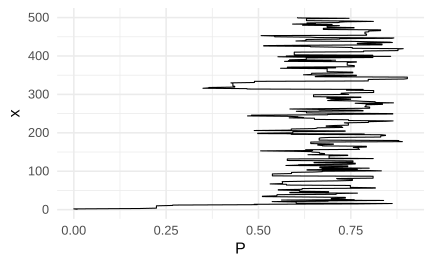
\includegraphics[width=0.7\linewidth]{Notas-Curso-Estadistica_files/figure-latex/unnamed-chunk-129-1} \end{center}

\begin{Shaded}
\begin{Highlighting}[]
\KeywordTok{ggplot}\NormalTok{(df[}\DecValTok{500}\OperatorTok{:}\NormalTok{n_pasos, ]) }\OperatorTok{+}\StringTok{ }\KeywordTok{geom_histogram}\NormalTok{(}\KeywordTok{aes}\NormalTok{(P, }\DataTypeTok{y =}\NormalTok{ ..density..), }
    \DataTypeTok{color =} \StringTok{"white"}\NormalTok{) }\OperatorTok{+}\StringTok{ }\KeywordTok{theme_minimal}\NormalTok{(}\DataTypeTok{base_size =} \DecValTok{16}\NormalTok{)}
\end{Highlighting}
\end{Shaded}

\begin{center}\includegraphics[width=0.7\linewidth]{Notas-Curso-Estadistica_files/figure-latex/unnamed-chunk-129-2} \end{center}

\hypertarget{dos-monedas}{%
\section{Dos monedas}\label{dos-monedas}}

Un problema con el algoritmo de Metropolis-Hastings (M-H) es que solo funciona para la estimación de un solo parámetro.

El muestreo de Gibbs está pensado en el caso de la estimación de muchos parámetros de forma bastante ordenada.

Supongamos que tenemos dos monedas y queremos ver la proporción de escudos generados entre las dos monedas:

Tenemos:

\begin{itemize}
\tightlist
\item
  Parámetros: \(\theta_{1}\) y \(\theta_{2}\).
\item
  Datos: \(N_{1}\) tiradas de la moneda 1 y \(N_{2}\) tiradas de la moneda 2. (cada una tuvo \(z_{1}\) y \(z_{2}\) éxitos).
\end{itemize}

\begin{enumerate}
\def\labelenumi{\arabic{enumi}.}
\setcounter{enumi}{2}
\item
  Verosimilitud: Bernoulli.
  \begin{equation*}
  y_{1}^{i}\sim \mathrm{Bernoulli}(\theta_{1}) 
  \quad 
  y_{2}^{i}\sim \mathrm{Bernoulli}(\theta_{2}) 
  \end{equation*}
\item
  Previa: Beta independiente para cada \(\theta\).
  \begin{equation*}
  \theta_{1}\sim \mathrm{Beta}(a_{1},b_{1}) 
  \quad 
  \theta_{2}\sim \mathrm{Beta}(a_{2},b_{2}) 
  \end{equation*}
\end{enumerate}

La distribución posterior se puede escribir como

\begin{align*}
f\left(\theta_{1}, \theta_{2} | D\right) 
&=f\left(D | \theta_{1}, \theta_{2}\right) \frac{f\left(\theta_{1}, \theta_{2}\right)}{f(D)} \\
&=\theta_{1}^{z_{1}}\left(1-\theta_{1}\right)^{N_{1}-z_{1}} \theta_{1}^{z_{2}}\left(1-\theta_{2}\right)^{N_{2}-z_{2}} \frac{f\left(\theta_{1}, \theta_{2}\right)}{f(D)}  \\
&=\frac{\theta_{1}^{z_{1}}\left(1-\theta_{1}\right)^{N_{1}-z_{1}} \theta_{1}^{z_{2}}\left(1-\theta_{2}\right)^{N_{2}-z_{2}} \theta_{1}^{a_{1}-1}\left(1-\theta_{1}\right)^{b_{1}-1} \theta_{2}^{a_{2}-1}\left(1-\theta_{2}\right)^{b_{2}-1}}{f(D) B\left(a_{1}, b_{1}\right) B\left(a_{2}, b_{2}\right)} \\
&=\frac{\theta_{1}^{z_{1}+a_{1}-1}\left(1-\theta_{1}\right)^{N_{1}-z_{1}+b_{1}-1} \theta_{2}^{z_{2}+a_{2}-1}\left(1-\theta_{2}\right)^{N_{2}-z_{2}+b_{2}-1}}{f(D) B\left(a_{1}, b_{1}\right) B\left(a_{2}, b_{2}\right)}
\end{align*}
Entonces la distribución posterior de \(\left(\theta_{1}, \theta_{2}\right)\) son dos distribuciones independientes Betas:
\(\operatorname{Beta}\left(z_{1}+a, N_{1}-z_{1}+b_{1}\right)\) y \(\operatorname{Beta}\left(z_{2}+a, N_{2}-z_{2}+b_{2}\right)\)

Tratemos de encontrar los parámetros para la distribución posterior usando un algoritmo de Metropolis-Hasting. \href{https://rpruim.github.io/Kruschke-Notes/markov-chain-monte-carlo-mcmc.html\#metropolis}{Función tomada de Kruschke-Notes}

\begin{Shaded}
\begin{Highlighting}[]
\NormalTok{metro_2coins <-}\StringTok{ }\ControlFlowTok{function}\NormalTok{(}
\NormalTok{  z1, n1,              }\CommentTok{# z = successes, n = trials}
\NormalTok{  z2, n2,              }\CommentTok{# z = successes, n = trials}
  \DataTypeTok{size  =} \KeywordTok{c}\NormalTok{(}\FloatTok{0.1}\NormalTok{, }\FloatTok{0.1}\NormalTok{), }\CommentTok{# sds of jump distribution}
  \DataTypeTok{start =} \KeywordTok{c}\NormalTok{(}\FloatTok{0.5}\NormalTok{, }\FloatTok{0.5}\NormalTok{), }\CommentTok{# value of thetas to start at}
  \DataTypeTok{num_steps =} \FloatTok{5e4}\NormalTok{,     }\CommentTok{# number of steps to run the algorithm}
  \DataTypeTok{prior1 =}\NormalTok{ dbeta,      }\CommentTok{# function describing prior}
  \DataTypeTok{prior2 =}\NormalTok{ dbeta,      }\CommentTok{# function describing prior}
  \DataTypeTok{args1 =} \KeywordTok{list}\NormalTok{(),      }\CommentTok{# additional args for prior1}
  \DataTypeTok{args2 =} \KeywordTok{list}\NormalTok{()      }\CommentTok{# additional args for prior2}
\NormalTok{  ) \{}
  
\NormalTok{  theta1            <-}\StringTok{ }\KeywordTok{rep}\NormalTok{(}\OtherTok{NA}\NormalTok{, num_steps)  }\CommentTok{# trick to pre-alocate memory}
\NormalTok{  theta2            <-}\StringTok{ }\KeywordTok{rep}\NormalTok{(}\OtherTok{NA}\NormalTok{, num_steps)  }\CommentTok{# trick to pre-alocate memory}
\NormalTok{  proposed_theta1   <-}\StringTok{ }\KeywordTok{rep}\NormalTok{(}\OtherTok{NA}\NormalTok{, num_steps)  }\CommentTok{# trick to pre-alocate memory}
\NormalTok{  proposed_theta2   <-}\StringTok{ }\KeywordTok{rep}\NormalTok{(}\OtherTok{NA}\NormalTok{, num_steps)  }\CommentTok{# trick to pre-alocate memory}
\NormalTok{  move              <-}\StringTok{ }\KeywordTok{rep}\NormalTok{(}\OtherTok{NA}\NormalTok{, num_steps)  }\CommentTok{# trick to pre-alocate memory}
\NormalTok{  theta1[}\DecValTok{1}\NormalTok{]         <-}\StringTok{ }\NormalTok{start[}\DecValTok{1}\NormalTok{]}
\NormalTok{  theta2[}\DecValTok{1}\NormalTok{]         <-}\StringTok{ }\NormalTok{start[}\DecValTok{2}\NormalTok{]}

\NormalTok{  size1 <-}\StringTok{ }\NormalTok{size[}\DecValTok{1}\NormalTok{] }
\NormalTok{  size2 <-}\StringTok{ }\NormalTok{size[}\DecValTok{2}\NormalTok{] }
  
  \ControlFlowTok{for}\NormalTok{ (i }\ControlFlowTok{in} \DecValTok{1}\OperatorTok{:}\NormalTok{(num_steps}\DecValTok{-1}\NormalTok{)) \{}
    \CommentTok{# head to new "island"}
\NormalTok{    proposed_theta1[i }\OperatorTok{+}\StringTok{ }\DecValTok{1}\NormalTok{] <-}\StringTok{ }\KeywordTok{rnorm}\NormalTok{(}\DecValTok{1}\NormalTok{, theta1[i], size1)}
\NormalTok{    proposed_theta2[i }\OperatorTok{+}\StringTok{ }\DecValTok{1}\NormalTok{] <-}\StringTok{ }\KeywordTok{rnorm}\NormalTok{(}\DecValTok{1}\NormalTok{, theta2[i], size2)}
    
    \ControlFlowTok{if}\NormalTok{ (proposed_theta1[i }\OperatorTok{+}\StringTok{ }\DecValTok{1}\NormalTok{] }\OperatorTok{<=}\StringTok{ }\DecValTok{0} \OperatorTok{||}
\StringTok{        }\NormalTok{proposed_theta1[i }\OperatorTok{+}\StringTok{ }\DecValTok{1}\NormalTok{] }\OperatorTok{>=}\StringTok{ }\DecValTok{1} \OperatorTok{||}
\StringTok{        }\NormalTok{proposed_theta2[i }\OperatorTok{+}\StringTok{ }\DecValTok{1}\NormalTok{] }\OperatorTok{<=}\StringTok{ }\DecValTok{0} \OperatorTok{||}
\StringTok{        }\NormalTok{proposed_theta2[i }\OperatorTok{+}\StringTok{ }\DecValTok{1}\NormalTok{] }\OperatorTok{>=}\StringTok{ }\DecValTok{1}\NormalTok{) \{}
\NormalTok{      proposed_posterior <-}\StringTok{ }\DecValTok{0}  \CommentTok{# because prior is 0}
\NormalTok{    \} }\ControlFlowTok{else}\NormalTok{ \{}
\NormalTok{      current_prior <-}\StringTok{ }
\StringTok{        }\KeywordTok{do.call}\NormalTok{(prior1, }\KeywordTok{c}\NormalTok{(}\KeywordTok{list}\NormalTok{(theta1[i]), args1)) }\OperatorTok{*}
\StringTok{        }\KeywordTok{do.call}\NormalTok{(prior2, }\KeywordTok{c}\NormalTok{(}\KeywordTok{list}\NormalTok{(theta2[i]), args2))}
\NormalTok{      current_likelihood  <-}\StringTok{ }
\StringTok{        }\KeywordTok{dbinom}\NormalTok{(z1, n1, theta1[i]) }\OperatorTok{*}
\StringTok{        }\KeywordTok{dbinom}\NormalTok{(z2, n2, theta2[i])}
\NormalTok{      current_posterior   <-}\StringTok{ }\NormalTok{current_prior }\OperatorTok{*}\StringTok{ }\NormalTok{current_likelihood}
      
\NormalTok{      proposed_prior <-}\StringTok{ }
\StringTok{        }\KeywordTok{do.call}\NormalTok{(prior1, }\KeywordTok{c}\NormalTok{(}\KeywordTok{list}\NormalTok{(proposed_theta1[i}\OperatorTok{+}\DecValTok{1}\NormalTok{]), args1)) }\OperatorTok{*}
\StringTok{        }\KeywordTok{do.call}\NormalTok{(prior2, }\KeywordTok{c}\NormalTok{(}\KeywordTok{list}\NormalTok{(proposed_theta2[i}\OperatorTok{+}\DecValTok{1}\NormalTok{]), args2))}
\NormalTok{      proposed_likelihood  <-}\StringTok{ }
\StringTok{        }\KeywordTok{dbinom}\NormalTok{(z1, n1, proposed_theta1[i}\OperatorTok{+}\DecValTok{1}\NormalTok{]) }\OperatorTok{*}
\StringTok{        }\KeywordTok{dbinom}\NormalTok{(z2, n2, proposed_theta2[i}\OperatorTok{+}\DecValTok{1}\NormalTok{])}
\NormalTok{      proposed_posterior   <-}\StringTok{ }\NormalTok{proposed_prior }\OperatorTok{*}\StringTok{ }\NormalTok{proposed_likelihood}
\NormalTok{    \}}
\NormalTok{    prob_move           <-}\StringTok{ }\NormalTok{proposed_posterior }\OperatorTok{/}\StringTok{ }\NormalTok{current_posterior}
    
    \CommentTok{# sometimes we "sail back"}
    \ControlFlowTok{if}\NormalTok{ (}\KeywordTok{runif}\NormalTok{(}\DecValTok{1}\NormalTok{) }\OperatorTok{>}\StringTok{ }\NormalTok{prob_move) \{ }\CommentTok{# sail back}
\NormalTok{       move[i }\OperatorTok{+}\StringTok{ }\DecValTok{1}\NormalTok{] <-}\StringTok{ }\OtherTok{FALSE}
\NormalTok{      theta1[i }\OperatorTok{+}\StringTok{ }\DecValTok{1}\NormalTok{] <-}\StringTok{ }\NormalTok{theta1[i]}
\NormalTok{      theta2[i }\OperatorTok{+}\StringTok{ }\DecValTok{1}\NormalTok{] <-}\StringTok{ }\NormalTok{theta2[i]}
\NormalTok{    \} }\ControlFlowTok{else}\NormalTok{ \{                    }\CommentTok{# stay}
\NormalTok{       move[i }\OperatorTok{+}\StringTok{ }\DecValTok{1}\NormalTok{] <-}\StringTok{ }\OtherTok{TRUE}
\NormalTok{      theta1[i }\OperatorTok{+}\StringTok{ }\DecValTok{1}\NormalTok{] <-}\StringTok{ }\NormalTok{proposed_theta1[i }\OperatorTok{+}\StringTok{ }\DecValTok{1}\NormalTok{]}
\NormalTok{      theta2[i }\OperatorTok{+}\StringTok{ }\DecValTok{1}\NormalTok{] <-}\StringTok{ }\NormalTok{proposed_theta2[i }\OperatorTok{+}\StringTok{ }\DecValTok{1}\NormalTok{]}
\NormalTok{    \}}
\NormalTok{  \}}
  
  \KeywordTok{tibble}\NormalTok{(}
    \DataTypeTok{step =} \DecValTok{1}\OperatorTok{:}\NormalTok{num_steps, }
    \DataTypeTok{theta1 =}\NormalTok{ theta1,}
    \DataTypeTok{theta2 =}\NormalTok{ theta2,}
    \DataTypeTok{proposed_theta1 =}\NormalTok{ proposed_theta1,}
    \DataTypeTok{proposed_theta2 =}\NormalTok{ proposed_theta2,}
    \DataTypeTok{move =}\NormalTok{ move, }
    \DataTypeTok{size1 =}\NormalTok{ size1,}
    \DataTypeTok{size2 =}\NormalTok{ size2}
\NormalTok{  )}
\NormalTok{\}}
\end{Highlighting}
\end{Shaded}

\begin{Shaded}
\begin{Highlighting}[]
\NormalTok{Metro_2coinsA <-}\StringTok{ }\KeywordTok{metro_2coins}\NormalTok{(}\DataTypeTok{z1 =} \DecValTok{6}\NormalTok{, }\DataTypeTok{n1 =} \DecValTok{8}\NormalTok{, }\DataTypeTok{z2 =} \DecValTok{2}\NormalTok{, }
    \DataTypeTok{n2 =} \DecValTok{7}\NormalTok{, }\DataTypeTok{size =} \KeywordTok{c}\NormalTok{(}\FloatTok{0.02}\NormalTok{, }\FloatTok{0.02}\NormalTok{), }\DataTypeTok{args1 =} \KeywordTok{list}\NormalTok{(}\DataTypeTok{shape1 =} \DecValTok{2}\NormalTok{, }
        \DataTypeTok{shape2 =} \DecValTok{2}\NormalTok{), }\DataTypeTok{args2 =} \KeywordTok{list}\NormalTok{(}\DataTypeTok{shape1 =} \DecValTok{2}\NormalTok{, }\DataTypeTok{shape2 =} \DecValTok{2}\NormalTok{))}

\NormalTok{Metro_2coinsA }\OperatorTok\StringTok{ }\KeywordTok{gf_density2d}\NormalTok{(theta2 }\OperatorTok{~}\StringTok{ }\NormalTok{theta1)}
\end{Highlighting}
\end{Shaded}

\begin{center}\includegraphics[width=0.7\linewidth]{Notas-Curso-Estadistica_files/figure-latex/unnamed-chunk-131-1} \end{center}

\begin{Shaded}
\begin{Highlighting}[]
\NormalTok{Metro_2coinsA }\OperatorTok\StringTok{ }\KeywordTok{gf_density}\NormalTok{(}\OperatorTok{~}\NormalTok{(theta2 }\OperatorTok{-}\StringTok{ }\NormalTok{theta1))}
\end{Highlighting}
\end{Shaded}

\begin{center}\includegraphics[width=0.7\linewidth]{Notas-Curso-Estadistica_files/figure-latex/unnamed-chunk-131-2} \end{center}

\begin{Shaded}
\begin{Highlighting}[]
\KeywordTok{acf}\NormalTok{(Metro_2coinsA}\OperatorTok{$}\NormalTok{theta2 }\OperatorTok{-}\StringTok{ }\NormalTok{Metro_2coinsA}\OperatorTok{$}\NormalTok{theta1)}
\end{Highlighting}
\end{Shaded}

\begin{center}\includegraphics[width=0.7\linewidth]{Notas-Curso-Estadistica_files/figure-latex/unnamed-chunk-131-3} \end{center}

\begin{Shaded}
\begin{Highlighting}[]
\NormalTok{Metro_2coinsA }\OperatorTok\StringTok{ }\KeywordTok{filter}\NormalTok{(step }\OperatorTok{<}\StringTok{ }\DecValTok{500}\NormalTok{) }\OperatorTok\StringTok{ }\KeywordTok{gf_path}\NormalTok{(theta2 }\OperatorTok{~}\StringTok{ }
\StringTok{    }\NormalTok{theta1, }\DataTypeTok{color =} \OperatorTok{~}\NormalTok{step, }\DataTypeTok{alpha =} \FloatTok{0.5}\NormalTok{, }\DataTypeTok{arrow =} \KeywordTok{arrow}\NormalTok{(}\DataTypeTok{type =} \StringTok{"open"}\NormalTok{, }
    \DataTypeTok{angle =} \DecValTok{30}\NormalTok{, }\DataTypeTok{length =} \KeywordTok{unit}\NormalTok{(}\FloatTok{0.1}\NormalTok{, }\StringTok{"inches"}\NormalTok{))) }\OperatorTok{+}\StringTok{ }\KeywordTok{theme_minimal}\NormalTok{()}
\end{Highlighting}
\end{Shaded}

\begin{center}\includegraphics[width=0.7\linewidth]{Notas-Curso-Estadistica_files/figure-latex/unnamed-chunk-132-1} \end{center}

\begin{Shaded}
\begin{Highlighting}[]
\KeywordTok{library}\NormalTok{(gganimate)}
\NormalTok{Metro_2coinsAplot <-}\StringTok{ }\NormalTok{Metro_2coinsA }\OperatorTok\StringTok{ }\KeywordTok{filter}\NormalTok{(step }\OperatorTok{<}\StringTok{ }
\StringTok{    }\DecValTok{500}\NormalTok{) }\OperatorTok\StringTok{ }\KeywordTok{gf_path}\NormalTok{(theta2 }\OperatorTok{~}\StringTok{ }\NormalTok{theta1, }\DataTypeTok{color =} \OperatorTok{~}\NormalTok{step, }
    \DataTypeTok{alpha =} \FloatTok{0.5}\NormalTok{, }\DataTypeTok{arrow =} \KeywordTok{arrow}\NormalTok{(}\DataTypeTok{type =} \StringTok{"open"}\NormalTok{, }\DataTypeTok{angle =} \DecValTok{30}\NormalTok{)) }\OperatorTok{+}\StringTok{ }
\StringTok{    }\KeywordTok{theme_minimal}\NormalTok{() }\OperatorTok{+}\StringTok{ }\KeywordTok{transition_reveal}\NormalTok{(step)}

\KeywordTok{animate}\NormalTok{(Metro_2coinsAplot, }\DataTypeTok{fps =} \DecValTok{1}\NormalTok{)}
\end{Highlighting}
\end{Shaded}

\begin{Shaded}
\begin{Highlighting}[]
\NormalTok{Metro_2coinsB <-}\StringTok{ }\KeywordTok{metro_2coins}\NormalTok{(}\DataTypeTok{z1 =} \DecValTok{6}\NormalTok{, }\DataTypeTok{n1 =} \DecValTok{8}\NormalTok{, }\DataTypeTok{z2 =} \DecValTok{2}\NormalTok{, }
    \DataTypeTok{n2 =} \DecValTok{7}\NormalTok{, }\DataTypeTok{size =} \KeywordTok{c}\NormalTok{(}\FloatTok{0.2}\NormalTok{, }\FloatTok{0.2}\NormalTok{), }\DataTypeTok{args1 =} \KeywordTok{list}\NormalTok{(}\DataTypeTok{shape1 =} \DecValTok{2}\NormalTok{, }
        \DataTypeTok{shape2 =} \DecValTok{2}\NormalTok{), }\DataTypeTok{args2 =} \KeywordTok{list}\NormalTok{(}\DataTypeTok{shape1 =} \DecValTok{2}\NormalTok{, }\DataTypeTok{shape2 =} \DecValTok{2}\NormalTok{))}

\NormalTok{Metro_2coinsB }\OperatorTok\StringTok{ }\KeywordTok{gf_density2d}\NormalTok{(theta2 }\OperatorTok{~}\StringTok{ }\NormalTok{theta1)}
\end{Highlighting}
\end{Shaded}

\begin{center}\includegraphics[width=0.7\linewidth]{Notas-Curso-Estadistica_files/figure-latex/unnamed-chunk-135-1} \end{center}

\begin{Shaded}
\begin{Highlighting}[]
\KeywordTok{acf}\NormalTok{(Metro_2coinsB}\OperatorTok{$}\NormalTok{theta2 }\OperatorTok{-}\StringTok{ }\NormalTok{Metro_2coinsB}\OperatorTok{$}\NormalTok{theta1)}
\end{Highlighting}
\end{Shaded}

\begin{center}\includegraphics[width=0.7\linewidth]{Notas-Curso-Estadistica_files/figure-latex/unnamed-chunk-135-2} \end{center}

\begin{Shaded}
\begin{Highlighting}[]
\NormalTok{Metro_2coinsB }\OperatorTok\StringTok{ }\KeywordTok{filter}\NormalTok{(step }\OperatorTok{<}\StringTok{ }\DecValTok{500}\NormalTok{) }\OperatorTok\StringTok{ }\KeywordTok{gf_path}\NormalTok{(theta2 }\OperatorTok{~}\StringTok{ }
\StringTok{    }\NormalTok{theta1, }\DataTypeTok{color =} \OperatorTok{~}\NormalTok{step, }\DataTypeTok{alpha =} \FloatTok{0.5}\NormalTok{, }\DataTypeTok{arrow =} \KeywordTok{arrow}\NormalTok{(}\DataTypeTok{type =} \StringTok{"open"}\NormalTok{, }
    \DataTypeTok{angle =} \DecValTok{30}\NormalTok{, }\DataTypeTok{length =} \KeywordTok{unit}\NormalTok{(}\FloatTok{0.1}\NormalTok{, }\StringTok{"inches"}\NormalTok{))) }\OperatorTok{+}\StringTok{ }\KeywordTok{theme_minimal}\NormalTok{()}
\end{Highlighting}
\end{Shaded}

\begin{center}\includegraphics[width=0.7\linewidth]{Notas-Curso-Estadistica_files/figure-latex/unnamed-chunk-136-1} \end{center}

\begin{Shaded}
\begin{Highlighting}[]
\NormalTok{Metro_2coinsBplot <-}\StringTok{ }\NormalTok{Metro_2coinsA }\OperatorTok\StringTok{ }\KeywordTok{filter}\NormalTok{(step }\OperatorTok{<}\StringTok{ }
\StringTok{    }\DecValTok{500}\NormalTok{) }\OperatorTok\StringTok{ }\KeywordTok{gf_path}\NormalTok{(theta2 }\OperatorTok{~}\StringTok{ }\NormalTok{theta1, }\DataTypeTok{color =} \OperatorTok{~}\NormalTok{step, }
    \DataTypeTok{alpha =} \FloatTok{0.5}\NormalTok{, }\DataTypeTok{arrow =} \KeywordTok{arrow}\NormalTok{(}\DataTypeTok{type =} \StringTok{"open"}\NormalTok{, }\DataTypeTok{angle =} \DecValTok{30}\NormalTok{)) }\OperatorTok{+}\StringTok{ }
\StringTok{    }\KeywordTok{theme_minimal}\NormalTok{() }\OperatorTok{+}\StringTok{ }\KeywordTok{transition_reveal}\NormalTok{(step)}

\KeywordTok{animate}\NormalTok{(Metro_2coinsBplot, }\DataTypeTok{fps =} \DecValTok{1}\NormalTok{)}
\end{Highlighting}
\end{Shaded}

\hypertarget{muestreo-de-gibbs}{%
\subsection{Muestreo de Gibbs}\label{muestreo-de-gibbs}}

Para este ejemplo \(\left( \theta_{1},\theta_{2} \right)\), entonces la forma de escoger la posteriores en cada paso sería de la forma:

\begin{enumerate}
\def\labelenumi{\arabic{enumi}.}
\tightlist
\item
  Tome al azar un \(\boldsymbol{\theta}^{0} = \left( \theta_{1}^{0},\theta_{2}^{0} \right)\).
\item
  Escoja \(\theta_{1}^{1}\) a partir de la distribución
  \(f\left(\theta_{1} \vert \theta_{1}=\theta_{1}^{0}, \theta_{2}=\theta_{2}^{0}, \boldsymbol{X} \right)\).
\item
  Escoja \(\theta_{2}^{1}\) a partir de la distribución
  \(f\left(\theta_{2} \vert \theta_{1}=\theta_{1}^{1}, \theta_{2}=\theta_{2}^{0}, \boldsymbol{X} \right)\).
\end{enumerate}

Esto completa un ciclo del muestreo. Cada ciclo genera nuevos \(\boldsymbol{\theta}^{i} = \left( \theta_{1}^{i},\theta_{2}^{i} \right)\) hasta que el proceso converja.

\BeginKnitrBlock{remark}
\iffalse{} {Nota: } \fi{}En realidad el muestreo de Gibbs se basa en el algoritmo de M-H, con la diferencia que la elección de los parámetros se escogen teniendo en cuanta los datos y fijando los otros parámetros. Es decir,

\begin{align*}
&{\left[\theta_{1} | \theta_{2}, \ldots, \theta_{M}, datos \right]} \\
&{\left[\theta_{2} | \theta_{1}, \theta_{3}, \ldots, \theta_{M}, datos \right]} \\
&{\left[\theta_{M} | \theta_{1}, \ldots, \theta_{M-1}, datos \right]}
\end{align*}
\EndKnitrBlock{remark}

El tratamiento teórico puede ser consultado \url{https://www.ece.iastate.edu/~namrata/EE527_Spring08/l4c.pdf\#page=16}

\begin{align*}
f\left(\theta_{1} | \theta_{2}, D\right) 
&= \frac{f\left(\theta_{1}, \theta_{2} | D\right)}{f\left(\theta_{2} | D\right)}  \\
&= \frac{f\left(\theta_{1}, \theta_{2} | D\right)}{\int f\left(\theta_{1}, \theta_{2} | D\right)d \theta_{1}}   \\
&=\frac{\operatorname{dbeta}\left(\theta_{1}, z_{1}+a_{1}, N_{1}-z_{1}+b_{1}\right) \cdot \operatorname{dbeta}\left(\theta_{2}, z_{2}+a_{2}, N_{2}-z_{2}+b_{2}\right)}{\int  \operatorname{dbeta}\left(\theta_{1}, z_{1}+a_{1}, N_{1}-z_{1}+b_{1}\right) \cdot \operatorname{dbeta}\left(\theta_{2} | z_{2}+a_{2}, N_{2}-z_{2}+b_{2}\right)d \theta_{1}} \\
&=\frac{\operatorname{dbeta}\left(\theta_{1}, z_{1}+a_{1}, N_{1}-z_{1}+b_{1}\right) \cdot \operatorname{dbeta}\left(\theta_{2}, z_{2}+a_{2}, N_{2}-z_{2}+b_{2}\right)}{\operatorname{dbeta}\left(\theta_{2} | z_{2}+a_{2}, N_{2}-z_{2}+b_{2}\right) \int  \operatorname{dbeta}\left(\theta_{1}, z_{1}+a_{1}, N_{1}-z_{1}+b_{1}\right)d \theta_{1}} \\
&=\frac{\operatorname{dbeta}\left(\theta_{1}, z_{1}+a_{1}, N_{1}-z_{1}+b_{1}\right)}{\int  \operatorname{dbeta}\left(\theta_{1}, z_{1}+a_{1}, N_{1}-z_{1}+b_{1}\right)d \theta_{1}} \\
&=\operatorname{dbeta}\left(\theta_{1}, z_{1}+a_{1}, N_{1}-z_{1}+b_{1}\right)
\end{align*}

\begin{Shaded}
\begin{Highlighting}[]
\NormalTok{gibbs_2coins <-}\StringTok{ }\ControlFlowTok{function}\NormalTok{(}
\NormalTok{  z1, n1,              }\CommentTok{# z = successes, n = trials}
\NormalTok{  z2, n2,              }\CommentTok{# z = successes, n = trials}
  \DataTypeTok{start =} \KeywordTok{c}\NormalTok{(}\FloatTok{0.5}\NormalTok{, }\FloatTok{0.5}\NormalTok{), }\CommentTok{# value of thetas to start at}
  \DataTypeTok{num_steps =} \FloatTok{1e4}\NormalTok{,     }\CommentTok{# number of steps to run the algorithm}
\NormalTok{  a1, b1,              }\CommentTok{# params for prior for theta1}
\NormalTok{  a2, b2               }\CommentTok{# params for prior for theta2}
\NormalTok{  ) \{}
  
\NormalTok{  theta1            <-}\StringTok{ }\KeywordTok{rep}\NormalTok{(}\OtherTok{NA}\NormalTok{, num_steps)  }\CommentTok{# trick to pre-alocate memory}
\NormalTok{  theta2            <-}\StringTok{ }\KeywordTok{rep}\NormalTok{(}\OtherTok{NA}\NormalTok{, num_steps)  }\CommentTok{# trick to pre-alocate memory}
\NormalTok{  theta1[}\DecValTok{1}\NormalTok{]         <-}\StringTok{ }\NormalTok{start[}\DecValTok{1}\NormalTok{]}
\NormalTok{  theta2[}\DecValTok{1}\NormalTok{]         <-}\StringTok{ }\NormalTok{start[}\DecValTok{2}\NormalTok{]}
  
  \ControlFlowTok{for}\NormalTok{ (i }\ControlFlowTok{in} \DecValTok{1}\OperatorTok{:}\NormalTok{(num_steps}\DecValTok{-1}\NormalTok{)) \{}
    \ControlFlowTok{if}\NormalTok{ (i }\OperatorTok\StringTok{ }\DecValTok{2} \OperatorTok{==}\StringTok{ }\DecValTok{1}\NormalTok{) \{ }\CommentTok{# update theta1}
\NormalTok{      theta1[i}\OperatorTok{+}\DecValTok{1}\NormalTok{] <-}\StringTok{ }\KeywordTok{rbeta}\NormalTok{(}\DecValTok{1}\NormalTok{, z1 }\OperatorTok{+}\StringTok{ }\NormalTok{a1, n1 }\OperatorTok{-}\StringTok{ }\NormalTok{z1 }\OperatorTok{+}\StringTok{ }\NormalTok{b1)}
\NormalTok{      theta2[i}\OperatorTok{+}\DecValTok{1}\NormalTok{] <-}\StringTok{ }\NormalTok{theta2[i]}
\NormalTok{    \} }\ControlFlowTok{else}\NormalTok{ \{           }\CommentTok{# update theta2}
\NormalTok{      theta1[i}\OperatorTok{+}\DecValTok{1}\NormalTok{] <-}\StringTok{ }\NormalTok{theta1[i]}
\NormalTok{      theta2[i}\OperatorTok{+}\DecValTok{1}\NormalTok{] <-}\StringTok{ }\KeywordTok{rbeta}\NormalTok{(}\DecValTok{1}\NormalTok{, z2 }\OperatorTok{+}\StringTok{ }\NormalTok{a2, n2 }\OperatorTok{-}\StringTok{ }\NormalTok{z2 }\OperatorTok{+}\StringTok{ }\NormalTok{b2)}
\NormalTok{    \}}
\NormalTok{  \}}
  
  \KeywordTok{tibble}\NormalTok{(}
    \DataTypeTok{step =} \DecValTok{1}\OperatorTok{:}\NormalTok{num_steps, }
    \DataTypeTok{theta1 =}\NormalTok{ theta1,}
    \DataTypeTok{theta2 =}\NormalTok{ theta2,}
\NormalTok{  )}
\NormalTok{\}}
\end{Highlighting}
\end{Shaded}

\begin{Shaded}
\begin{Highlighting}[]
\NormalTok{Gibbs <-}\StringTok{ }\KeywordTok{gibbs_2coins}\NormalTok{(}\DataTypeTok{z1 =} \DecValTok{6}\NormalTok{, }\DataTypeTok{n1 =} \DecValTok{8}\NormalTok{, }\DataTypeTok{z2 =} \DecValTok{2}\NormalTok{, }\DataTypeTok{n2 =} \DecValTok{7}\NormalTok{, }
    \DataTypeTok{a1 =} \DecValTok{2}\NormalTok{, }\DataTypeTok{b1 =} \DecValTok{2}\NormalTok{, }\DataTypeTok{a2 =} \DecValTok{2}\NormalTok{, }\DataTypeTok{b2 =} \DecValTok{2}\NormalTok{)}

\NormalTok{Gibbs }\OperatorTok\StringTok{ }\KeywordTok{gf_density2d}\NormalTok{(theta2 }\OperatorTok{~}\StringTok{ }\NormalTok{theta1)}
\end{Highlighting}
\end{Shaded}

\begin{center}\includegraphics[width=0.7\linewidth]{Notas-Curso-Estadistica_files/figure-latex/unnamed-chunk-140-1} \end{center}

\begin{Shaded}
\begin{Highlighting}[]
\NormalTok{Gibbs }\OperatorTok\StringTok{ }\KeywordTok{gf_dens}\NormalTok{(}\OperatorTok{~}\NormalTok{theta1)}
\end{Highlighting}
\end{Shaded}

\begin{center}\includegraphics[width=0.7\linewidth]{Notas-Curso-Estadistica_files/figure-latex/unnamed-chunk-140-2} \end{center}

\begin{Shaded}
\begin{Highlighting}[]
\KeywordTok{acf}\NormalTok{(Gibbs}\OperatorTok{$}\NormalTok{theta1)}
\end{Highlighting}
\end{Shaded}

\begin{center}\includegraphics[width=0.7\linewidth]{Notas-Curso-Estadistica_files/figure-latex/unnamed-chunk-140-3} \end{center}

\begin{Shaded}
\begin{Highlighting}[]
\NormalTok{Gibbs }\OperatorTok\StringTok{ }\KeywordTok{filter}\NormalTok{(step }\OperatorTok{<}\StringTok{ }\DecValTok{500}\NormalTok{) }\OperatorTok\StringTok{ }\KeywordTok{gf_path}\NormalTok{(theta2 }\OperatorTok{~}\StringTok{ }\NormalTok{theta1, }
    \DataTypeTok{color =} \OperatorTok{~}\NormalTok{step, }\DataTypeTok{alpha =} \FloatTok{0.5}\NormalTok{, }\DataTypeTok{arrow =} \KeywordTok{arrow}\NormalTok{(}\DataTypeTok{type =} \StringTok{"open"}\NormalTok{, }
        \DataTypeTok{angle =} \DecValTok{30}\NormalTok{, }\DataTypeTok{length =} \KeywordTok{unit}\NormalTok{(}\FloatTok{0.1}\NormalTok{, }\StringTok{"inches"}\NormalTok{))) }\OperatorTok{+}\StringTok{ }
\StringTok{    }\KeywordTok{theme_minimal}\NormalTok{()}
\end{Highlighting}
\end{Shaded}

\begin{center}\includegraphics[width=0.7\linewidth]{Notas-Curso-Estadistica_files/figure-latex/unnamed-chunk-141-1} \end{center}

\begin{Shaded}
\begin{Highlighting}[]
\NormalTok{Gibbsplot <-}\StringTok{ }\NormalTok{Gibbs }\OperatorTok\StringTok{ }\KeywordTok{filter}\NormalTok{(step }\OperatorTok{<}\StringTok{ }\DecValTok{500}\NormalTok{) }\OperatorTok\StringTok{ }\KeywordTok{gf_path}\NormalTok{(theta2 }\OperatorTok{~}\StringTok{ }
\StringTok{    }\NormalTok{theta1, }\DataTypeTok{color =} \OperatorTok{~}\NormalTok{step, }\DataTypeTok{alpha =} \FloatTok{0.5}\NormalTok{, }\DataTypeTok{arrow =} \KeywordTok{arrow}\NormalTok{(}\DataTypeTok{type =} \StringTok{"open"}\NormalTok{, }
    \DataTypeTok{angle =} \DecValTok{30}\NormalTok{)) }\OperatorTok{+}\StringTok{ }\KeywordTok{theme_minimal}\NormalTok{() }\OperatorTok{+}\StringTok{ }\KeywordTok{transition_reveal}\NormalTok{(step)}

\KeywordTok{animate}\NormalTok{(Gibbsplot, }\DataTypeTok{fps =} \DecValTok{1}\NormalTok{)}
\end{Highlighting}
\end{Shaded}

Ciclos completos

\begin{Shaded}
\begin{Highlighting}[]
\NormalTok{Gibbs }\OperatorTok\StringTok{ }\KeywordTok{filter}\NormalTok{(step}\OperatorTok\DecValTok{2} \OperatorTok{==}\StringTok{ }\DecValTok{0}\NormalTok{) }\OperatorTok\StringTok{ }\KeywordTok{gf_density2d}\NormalTok{(theta2 }\OperatorTok{~}\StringTok{ }
\StringTok{    }\NormalTok{theta1)}
\end{Highlighting}
\end{Shaded}

\begin{center}\includegraphics[width=0.7\linewidth]{Notas-Curso-Estadistica_files/figure-latex/unnamed-chunk-143-1} \end{center}

\begin{Shaded}
\begin{Highlighting}[]
\NormalTok{Gibbs }\OperatorTok\StringTok{ }\KeywordTok{filter}\NormalTok{(step}\OperatorTok\DecValTok{2} \OperatorTok{==}\StringTok{ }\DecValTok{0}\NormalTok{) }\OperatorTok\StringTok{ }\KeywordTok{gf_density}\NormalTok{(}\OperatorTok{~}\NormalTok{(theta2 }\OperatorTok{-}\StringTok{ }
\StringTok{    }\NormalTok{theta1))}
\end{Highlighting}
\end{Shaded}

\begin{center}\includegraphics[width=0.7\linewidth]{Notas-Curso-Estadistica_files/figure-latex/unnamed-chunk-143-2} \end{center}

\begin{Shaded}
\begin{Highlighting}[]
\NormalTok{Gibbs }\OperatorTok\StringTok{ }\KeywordTok{filter}\NormalTok{(step}\OperatorTok\DecValTok{2} \OperatorTok{==}\StringTok{ }\DecValTok{0}\NormalTok{) }\OperatorTok\StringTok{ }\KeywordTok{mutate}\NormalTok{(}\DataTypeTok{difference =}\NormalTok{ theta2 }\OperatorTok{-}\StringTok{ }
\StringTok{    }\NormalTok{theta1) }\OperatorTok\StringTok{ }\KeywordTok{pull}\NormalTok{(difference) }\OperatorTok\StringTok{ }\KeywordTok{acf}\NormalTok{()}
\end{Highlighting}
\end{Shaded}

\begin{center}\includegraphics[width=0.7\linewidth]{Notas-Curso-Estadistica_files/figure-latex/unnamed-chunk-143-3} \end{center}

\begin{Shaded}
\begin{Highlighting}[]
\NormalTok{Gibbs }\OperatorTok\StringTok{ }\KeywordTok{filter}\NormalTok{(step }\OperatorTok{<}\StringTok{ }\DecValTok{500}\NormalTok{, step}\OperatorTok\DecValTok{2} \OperatorTok{==}\StringTok{ }\DecValTok{0}\NormalTok{) }\OperatorTok\StringTok{ }\KeywordTok{gf_path}\NormalTok{(theta2 }\OperatorTok{~}\StringTok{ }
\StringTok{    }\NormalTok{theta1, }\DataTypeTok{color =} \OperatorTok{~}\NormalTok{step, }\DataTypeTok{alpha =} \FloatTok{0.5}\NormalTok{, }\DataTypeTok{arrow =} \KeywordTok{arrow}\NormalTok{(}\DataTypeTok{type =} \StringTok{"open"}\NormalTok{, }
    \DataTypeTok{angle =} \DecValTok{30}\NormalTok{, }\DataTypeTok{length =} \KeywordTok{unit}\NormalTok{(}\FloatTok{0.1}\NormalTok{, }\StringTok{"inches"}\NormalTok{))) }\OperatorTok{+}\StringTok{ }\KeywordTok{theme_minimal}\NormalTok{()}
\end{Highlighting}
\end{Shaded}

\begin{center}\includegraphics[width=0.7\linewidth]{Notas-Curso-Estadistica_files/figure-latex/unnamed-chunk-144-1} \end{center}

\begin{Shaded}
\begin{Highlighting}[]
\NormalTok{Gibbsplot2 <-}\StringTok{ }\NormalTok{Gibbs }\OperatorTok\StringTok{ }\KeywordTok{filter}\NormalTok{(step }\OperatorTok{<}\StringTok{ }\DecValTok{500}\NormalTok{, step}\OperatorTok\DecValTok{2} \OperatorTok{==}\StringTok{ }
\StringTok{    }\DecValTok{0}\NormalTok{) }\OperatorTok\StringTok{ }\KeywordTok{gf_path}\NormalTok{(theta2 }\OperatorTok{~}\StringTok{ }\NormalTok{theta1, }\DataTypeTok{color =} \OperatorTok{~}\NormalTok{step, }
    \DataTypeTok{alpha =} \FloatTok{0.5}\NormalTok{, }\DataTypeTok{arrow =} \KeywordTok{arrow}\NormalTok{(}\DataTypeTok{type =} \StringTok{"open"}\NormalTok{, }\DataTypeTok{angle =} \DecValTok{30}\NormalTok{)) }\OperatorTok{+}\StringTok{ }
\StringTok{    }\KeywordTok{theme_minimal}\NormalTok{() }\OperatorTok{+}\StringTok{ }\KeywordTok{transition_reveal}\NormalTok{(step)}

\KeywordTok{animate}\NormalTok{(Gibbsplot2, }\DataTypeTok{fps =} \DecValTok{1}\NormalTok{)}
\end{Highlighting}
\end{Shaded}

\hypertarget{uso-de-jags}{%
\section{Uso de JAGS}\label{uso-de-jags}}

El paquete que usaremos en esta sección es \texttt{R2jags} y \texttt{coda}. Los cargamos con las instrucciones

\begin{Shaded}
\begin{Highlighting}[]
\NormalTok{remotes}\OperatorTok{::}\KeywordTok{install_github}\NormalTok{(}\StringTok{"rpruim/CalvinBayes"}\NormalTok{)}
\end{Highlighting}
\end{Shaded}

\begin{Shaded}
\begin{Highlighting}[]
\KeywordTok{library}\NormalTok{(R2jags)}
\KeywordTok{library}\NormalTok{(coda)}
\KeywordTok{library}\NormalTok{(CalvinBayes)}
\end{Highlighting}
\end{Shaded}

\begin{Shaded}
\begin{Highlighting}[]
\NormalTok{bernoulli <-}\StringTok{ }\KeywordTok{read.csv}\NormalTok{(}\DataTypeTok{file =} \StringTok{"data/bernoulli.csv"}\NormalTok{, }
    \DataTypeTok{sep =} \StringTok{""}\NormalTok{)}
\NormalTok{tibble}\OperatorTok{::}\KeywordTok{glimpse}\NormalTok{(bernoulli)}
\end{Highlighting}
\end{Shaded}

\begin{verbatim}
## Rows: 50
## Columns: 1
## $ y <int> 0, 1, 0, 0, 0, 0, 0, 0, 0, 0, 1, 0, 0, 0, 1, 1, 1, 0, 0, 1, 0, 0,...
\end{verbatim}

\begin{Shaded}
\begin{Highlighting}[]
\KeywordTok{mean}\NormalTok{(bernoulli}\OperatorTok{$}\NormalTok{y)}
\end{Highlighting}
\end{Shaded}

\begin{verbatim}
## [1] 0.3
\end{verbatim}

\begin{Shaded}
\begin{Highlighting}[]
\KeywordTok{sd}\NormalTok{(bernoulli}\OperatorTok{$}\NormalTok{y)}
\end{Highlighting}
\end{Shaded}

\begin{verbatim}
## [1] 0.46291
\end{verbatim}

En el lenguaje usual de JAGS, el modelo debe escribirse de la forma:

\begin{verbatim}
model
{
    for (i in 1:N) {
        y[i] ~ dbern(theta)
    }
    theta ~ dbeta(1, 1)
}
\end{verbatim}

donde \texttt{dbern} y \texttt{dbeta} son las densidades de una bernoulli y beta respectivamente. En este lenguage no existen versiones vectorizadas de las funciones por lo que todo debe llenarse usando \texttt{for}'s. Una revisión completa de este lenguage la pueden econtrar en su manual de uso \footnote{\url{http://web.sgh.waw.pl/~atoroj/ekonometria_bayesowska/jags_user_manual.pdf}}

El paquete \texttt{R2jags} tiene la capacidad que en lugar de usar este tipo de sintaxis, se pueda usar el lenguaje natural para escribir el modelo. Note el uso de \texttt{function} en este caso.

\begin{Shaded}
\begin{Highlighting}[]
\NormalTok{bern_model <-}\StringTok{ }\ControlFlowTok{function}\NormalTok{() \{}
    \ControlFlowTok{for}\NormalTok{ (i }\ControlFlowTok{in} \DecValTok{1}\OperatorTok{:}\NormalTok{N) \{}
\NormalTok{        y[i] }\OperatorTok{~}\StringTok{ }\KeywordTok{dbern}\NormalTok{(theta)}
\NormalTok{    \}}
\NormalTok{    theta }\OperatorTok{~}\StringTok{ }\KeywordTok{dbeta}\NormalTok{(}\DecValTok{1}\NormalTok{, }\DecValTok{1}\NormalTok{)}
\NormalTok{\}}
\end{Highlighting}
\end{Shaded}

\begin{Shaded}
\begin{Highlighting}[]
\NormalTok{bern_jags <-}\StringTok{ }\KeywordTok{jags}\NormalTok{(}\DataTypeTok{data =} \KeywordTok{list}\NormalTok{(}\DataTypeTok{y =}\NormalTok{ bernoulli}\OperatorTok{$}\NormalTok{y, }\DataTypeTok{N =} \KeywordTok{nrow}\NormalTok{(bernoulli)), }
    \DataTypeTok{model.file =}\NormalTok{ bern_model, }\DataTypeTok{parameters.to.save =} \KeywordTok{c}\NormalTok{(}\StringTok{"theta"}\NormalTok{))}
\end{Highlighting}
\end{Shaded}

\begin{verbatim}
## Compiling model graph
##    Resolving undeclared variables
##    Allocating nodes
## Graph information:
##    Observed stochastic nodes: 50
##    Unobserved stochastic nodes: 1
##    Total graph size: 53
## 
## Initializing model
\end{verbatim}

Veamos el resultado

\begin{Shaded}
\begin{Highlighting}[]
\NormalTok{bern_jags}
\end{Highlighting}
\end{Shaded}

\begin{verbatim}
## Inference for Bugs model at "/tmp/RtmpEEWzw4/model7d129f359c9.txt", fit using jags,
##  3 chains, each with 2000 iterations (first 1000 discarded)
##  n.sims = 3000 iterations saved
##          mu.vect sd.vect   2.5%    25%    50%    75%  97.5%  Rhat n.eff
## theta      0.307   0.064  0.189  0.264  0.305  0.349  0.438 1.001  3000
## deviance  62.069   1.368 61.087 61.189 61.530 62.403 65.725 1.001  3000
## 
## For each parameter, n.eff is a crude measure of effective sample size,
## and Rhat is the potential scale reduction factor (at convergence, Rhat=1).
## 
## DIC info (using the rule, pD = var(deviance)/2)
## pD = 0.9 and DIC = 63.0
## DIC is an estimate of expected predictive error (lower deviance is better).
\end{verbatim}

\begin{Shaded}
\begin{Highlighting}[]
\KeywordTok{head}\NormalTok{(}\KeywordTok{posterior}\NormalTok{(bern_jags))}
\end{Highlighting}
\end{Shaded}

\begin{verbatim}
## Error in verosimilitud(theta, data): argument "data" is missing, with no default
\end{verbatim}

\begin{Shaded}
\begin{Highlighting}[]
\KeywordTok{gf_dhistogram}\NormalTok{(}\OperatorTok{~}\NormalTok{theta, }\DataTypeTok{data =} \KeywordTok{posterior}\NormalTok{(bern_jags), }
    \DataTypeTok{bins =} \DecValTok{50}\NormalTok{) }\OperatorTok\StringTok{ }\KeywordTok{gf_dens}\NormalTok{(}\OperatorTok{~}\NormalTok{theta, }\DataTypeTok{size =} \FloatTok{1.5}\NormalTok{, }\DataTypeTok{alpha =} \FloatTok{0.8}\NormalTok{) }\OperatorTok\StringTok{ }
\StringTok{    }\KeywordTok{gf_dist}\NormalTok{(}\StringTok{"beta"}\NormalTok{, }\DataTypeTok{shape1 =} \DecValTok{16}\NormalTok{, }\DataTypeTok{shape2 =} \DecValTok{36}\NormalTok{, }\DataTypeTok{color =} \StringTok{"red"}\NormalTok{)}
\end{Highlighting}
\end{Shaded}

\begin{verbatim}
## Error in verosimilitud(theta, data): argument "data" is missing, with no default
\end{verbatim}

\begin{Shaded}
\begin{Highlighting}[]
\NormalTok{bern_mcmc <-}\StringTok{ }\KeywordTok{as.mcmc}\NormalTok{(bern_jags)}
\KeywordTok{plot}\NormalTok{(bern_mcmc)}
\end{Highlighting}
\end{Shaded}

\begin{center}\includegraphics[width=0.7\linewidth]{Notas-Curso-Estadistica_files/figure-latex/unnamed-chunk-154-1} \end{center}

\begin{Shaded}
\begin{Highlighting}[]
\KeywordTok{library}\NormalTok{(bayesplot)}
\KeywordTok{mcmc_areas}\NormalTok{(bern_mcmc, }\DataTypeTok{pars =} \KeywordTok{c}\NormalTok{(}\StringTok{"theta"}\NormalTok{), }\DataTypeTok{prob =} \FloatTok{0.9}\NormalTok{)}
\end{Highlighting}
\end{Shaded}

\begin{center}\includegraphics[width=0.7\linewidth]{Notas-Curso-Estadistica_files/figure-latex/unnamed-chunk-155-1} \end{center}

\begin{Shaded}
\begin{Highlighting}[]
\KeywordTok{mcmc_trace}\NormalTok{(bern_mcmc, }\DataTypeTok{pars =} \StringTok{"theta"}\NormalTok{)}
\end{Highlighting}
\end{Shaded}

\begin{center}\includegraphics[width=0.7\linewidth]{Notas-Curso-Estadistica_files/figure-latex/unnamed-chunk-156-1} \end{center}

\begin{Shaded}
\begin{Highlighting}[]
\KeywordTok{mcmc_trace}\NormalTok{(bern_mcmc, }\DataTypeTok{pars =} \StringTok{"theta"}\NormalTok{) }\OperatorTok\StringTok{ }\KeywordTok{gf_facet_grid}\NormalTok{(Chain }\OperatorTok{~}\StringTok{ }
\StringTok{    }\NormalTok{.) }\OperatorTok\StringTok{ }\KeywordTok{gf_refine}\NormalTok{(}\KeywordTok{scale_color_viridis_d}\NormalTok{())}
\end{Highlighting}
\end{Shaded}

\begin{verbatim}
## Error: At least one layer must contain all faceting variables: `Chain`.
## * Plot is missing `Chain`
## * Layer 1 is missing `Chain`
\end{verbatim}

\begin{center}\includegraphics[width=0.7\linewidth]{Notas-Curso-Estadistica_files/figure-latex/unnamed-chunk-157-1} \end{center}

\begin{Shaded}
\begin{Highlighting}[]
\KeywordTok{plot_post}\NormalTok{(bern_mcmc[, }\StringTok{"theta"}\NormalTok{], }\DataTypeTok{main =} \StringTok{"theta"}\NormalTok{, }\DataTypeTok{xlab =} \KeywordTok{expression}\NormalTok{(theta), }
    \DataTypeTok{cenTend =} \StringTok{"median"}\NormalTok{, }\DataTypeTok{compVal =} \FloatTok{0.5}\NormalTok{, }\DataTypeTok{ROPE =} \KeywordTok{c}\NormalTok{(}\FloatTok{0.45}\NormalTok{, }
        \FloatTok{0.55}\NormalTok{), }\DataTypeTok{credMass =} \FloatTok{0.9}\NormalTok{, }\DataTypeTok{quietly =} \OtherTok{TRUE}\NormalTok{)}
\end{Highlighting}
\end{Shaded}

\begin{center}\includegraphics[width=0.7\linewidth]{Notas-Curso-Estadistica_files/figure-latex/unnamed-chunk-158-1} \end{center}

\begin{Shaded}
\begin{Highlighting}[]
\NormalTok{twobernoulli <-}\StringTok{ }\KeywordTok{read.csv}\NormalTok{(}\StringTok{"data/2bernoulli.csv"}\NormalTok{)}

\NormalTok{knitr}\OperatorTok{::}\KeywordTok{kable}\NormalTok{(twobernoulli)}
\end{Highlighting}
\end{Shaded}

\begin{tabular}{r|l}
\hline
y & s\\
\hline
1 & Reginald\\
\hline
0 & Reginald\\
\hline
1 & Reginald\\
\hline
1 & Reginald\\
\hline
1 & Reginald\\
\hline
1 & Reginald\\
\hline
1 & Reginald\\
\hline
0 & Reginald\\
\hline
0 & Tony\\
\hline
0 & Tony\\
\hline
1 & Tony\\
\hline
0 & Tony\\
\hline
0 & Tony\\
\hline
1 & Tony\\
\hline
0 & Tony\\
\hline
\end{tabular}

\begin{Shaded}
\begin{Highlighting}[]
\NormalTok{Target <-}\StringTok{ }\NormalTok{twobernoulli }\OperatorTok\StringTok{ }\KeywordTok{rename}\NormalTok{(}\DataTypeTok{hit =}\NormalTok{ y, }\DataTypeTok{subject =}\NormalTok{ s)}

\NormalTok{Target }\OperatorTok\StringTok{ }\KeywordTok{group_by}\NormalTok{(subject) }\OperatorTok\StringTok{ }\KeywordTok{summarise}\NormalTok{(}\DataTypeTok{prop_0 =} \KeywordTok{sum}\NormalTok{(}\DecValTok{1} \OperatorTok{-}\StringTok{ }
\StringTok{    }\NormalTok{hit)}\OperatorTok{/}\KeywordTok{n}\NormalTok{(), }\DataTypeTok{prop_1 =} \KeywordTok{sum}\NormalTok{(hit)}\OperatorTok{/}\KeywordTok{n}\NormalTok{(), }\DataTypeTok{attemps =} \KeywordTok{n}\NormalTok{())}
\end{Highlighting}
\end{Shaded}

\begin{verbatim}
## # A tibble: 2 x 4
##   subject  prop_0 prop_1 attemps
##   <chr>     <dbl>  <dbl>   <int>
## 1 Reginald  0.25   0.75        8
## 2 Tony      0.714  0.286       7
\end{verbatim}

\begin{Shaded}
\begin{Highlighting}[]
\NormalTok{bern2_model <-}\StringTok{ }\ControlFlowTok{function}\NormalTok{() \{}
    \ControlFlowTok{for}\NormalTok{ (i }\ControlFlowTok{in} \DecValTok{1}\OperatorTok{:}\NormalTok{Nobs) \{}
        \CommentTok{# each response is Bernoulli with the appropriate}
        \CommentTok{# theta}
\NormalTok{        hit[i] }\OperatorTok{~}\StringTok{ }\KeywordTok{dbern}\NormalTok{(theta[subject[i]])}
\NormalTok{    \}}
    \ControlFlowTok{for}\NormalTok{ (s }\ControlFlowTok{in} \DecValTok{1}\OperatorTok{:}\NormalTok{Nsub) \{}
\NormalTok{        theta[s] }\OperatorTok{~}\StringTok{ }\KeywordTok{dbeta}\NormalTok{(}\DecValTok{2}\NormalTok{, }\DecValTok{2}\NormalTok{)  }\CommentTok{# prior for each theta}
\NormalTok{    \}}
\NormalTok{\}}
\end{Highlighting}
\end{Shaded}

\begin{Shaded}
\begin{Highlighting}[]
\NormalTok{TargetList <-}\StringTok{ }\KeywordTok{list}\NormalTok{(}\DataTypeTok{Nobs =} \KeywordTok{nrow}\NormalTok{(Target), }\DataTypeTok{Nsub =} \DecValTok{2}\NormalTok{, }\DataTypeTok{hit =}\NormalTok{ Target}\OperatorTok{$}\NormalTok{hit, }
    \DataTypeTok{subject =} \KeywordTok{as.numeric}\NormalTok{(}\KeywordTok{as.factor}\NormalTok{(Target}\OperatorTok{$}\NormalTok{subject)))}
\NormalTok{TargetList}
\end{Highlighting}
\end{Shaded}

\begin{verbatim}
## $Nobs
## [1] 15
## 
## $Nsub
## [1] 2
## 
## $hit
##  [1] 1 0 1 1 1 1 1 0 0 0 1 0 0 1 0
## 
## $subject
##  [1] 1 1 1 1 1 1 1 1 2 2 2 2 2 2 2
\end{verbatim}

\begin{Shaded}
\begin{Highlighting}[]
\NormalTok{bern2_jags <-}\StringTok{ }\KeywordTok{jags}\NormalTok{(}\DataTypeTok{data =}\NormalTok{ TargetList, }\DataTypeTok{model =}\NormalTok{ bern2_model, }
    \DataTypeTok{parameters.to.save =} \StringTok{"theta"}\NormalTok{)}
\end{Highlighting}
\end{Shaded}

\begin{verbatim}
## Compiling model graph
##    Resolving undeclared variables
##    Allocating nodes
## Graph information:
##    Observed stochastic nodes: 15
##    Unobserved stochastic nodes: 2
##    Total graph size: 35
## 
## Initializing model
\end{verbatim}

\begin{Shaded}
\begin{Highlighting}[]
\NormalTok{bern2_mcmc <-}\StringTok{ }\KeywordTok{as.mcmc}\NormalTok{(bern2_jags)}

\KeywordTok{mcmc_acf}\NormalTok{(bern2_mcmc)}
\end{Highlighting}
\end{Shaded}

\begin{center}\includegraphics[width=0.7\linewidth]{Notas-Curso-Estadistica_files/figure-latex/unnamed-chunk-163-1} \end{center}

\begin{Shaded}
\begin{Highlighting}[]
\KeywordTok{mcmc_combo}\NormalTok{(bern2_mcmc, }\DataTypeTok{combo =} \KeywordTok{c}\NormalTok{(}\StringTok{"dens"}\NormalTok{, }\StringTok{"dens_overlay"}\NormalTok{, }
    \StringTok{"trace"}\NormalTok{, }\StringTok{"scatter"}\NormalTok{), }\DataTypeTok{pars =} \KeywordTok{c}\NormalTok{(}\StringTok{"theta[1]"}\NormalTok{, }\StringTok{"theta[2]"}\NormalTok{))}
\end{Highlighting}
\end{Shaded}

\begin{center}\includegraphics[width=0.7\linewidth]{Notas-Curso-Estadistica_files/figure-latex/unnamed-chunk-163-2} \end{center}

\hypertarget{uso-de-stan}{%
\section{Uso de STAN}\label{uso-de-stan}}

STAN\footnote{\url{https://mc-stan.org/}} es otro tipo de lenguaje para definir modelos bayesiano. El lenguaje es un poco más sencillo, pero es particularmente útil para modelos bastante complejos.

STAN no usa el muestreo de Gibbs, sino en el método de Monte-Carlo Hamiltoniano. En el artículo \autocite{Hoffman2014} se propone el método NUTS para mejorar el muestreo de Gibbs.

En este curso no nos referiremos a este procedimiento, pero si veremos un poco de la sintaxis del lenguaje STAN.

\begin{verbatim}
data {
  int<lower=0> N;               // number of trials
  int<lower=0, upper=1> y[N];   // success on trial n
}

parameters {
  real<lower=0, upper=1> theta; // chance of success
}

model {
  theta ~ uniform(0, 1);        // prior
  y ~ bernoulli(theta);         // likelihood
}
\end{verbatim}

\begin{Shaded}
\begin{Highlighting}[]
\KeywordTok{library}\NormalTok{(rstan)}

\NormalTok{fit <-}\StringTok{ }\KeywordTok{stan}\NormalTok{(}\DataTypeTok{model_code =}\NormalTok{ bern_stan}\OperatorTok{@}\NormalTok{model_code, }\DataTypeTok{data =} \KeywordTok{list}\NormalTok{(}\DataTypeTok{y =}\NormalTok{ bernoulli}\OperatorTok{$}\NormalTok{y, }
    \DataTypeTok{N =} \KeywordTok{nrow}\NormalTok{(bernoulli)), }\DataTypeTok{iter =} \DecValTok{5000}\NormalTok{)}
\end{Highlighting}
\end{Shaded}

\begin{verbatim}
## 
## SAMPLING FOR MODEL '4584de91ce47196187979d2da8a67926' NOW (CHAIN 1).
## Chain 1: 
## Chain 1: Gradient evaluation took 1.3e-05 seconds
## Chain 1: 1000 transitions using 10 leapfrog steps per transition would take 0.13 seconds.
## Chain 1: Adjust your expectations accordingly!
## Chain 1: 
## Chain 1: 
## Chain 1: Iteration:    1 / 5000 [  0%]  (Warmup)
## Chain 1: Iteration:  500 / 5000 [ 10%]  (Warmup)
## Chain 1: Iteration: 1000 / 5000 [ 20%]  (Warmup)
## Chain 1: Iteration: 1500 / 5000 [ 30%]  (Warmup)
## Chain 1: Iteration: 2000 / 5000 [ 40%]  (Warmup)
## Chain 1: Iteration: 2500 / 5000 [ 50%]  (Warmup)
## Chain 1: Iteration: 2501 / 5000 [ 50%]  (Sampling)
## Chain 1: Iteration: 3000 / 5000 [ 60%]  (Sampling)
## Chain 1: Iteration: 3500 / 5000 [ 70%]  (Sampling)
## Chain 1: Iteration: 4000 / 5000 [ 80%]  (Sampling)
## Chain 1: Iteration: 4500 / 5000 [ 90%]  (Sampling)
## Chain 1: Iteration: 5000 / 5000 [100%]  (Sampling)
## Chain 1: 
## Chain 1:  Elapsed Time: 0.014946 seconds (Warm-up)
## Chain 1:                0.016413 seconds (Sampling)
## Chain 1:                0.031359 seconds (Total)
## Chain 1: 
## 
## SAMPLING FOR MODEL '4584de91ce47196187979d2da8a67926' NOW (CHAIN 2).
## Chain 2: 
## Chain 2: Gradient evaluation took 1.3e-05 seconds
## Chain 2: 1000 transitions using 10 leapfrog steps per transition would take 0.13 seconds.
## Chain 2: Adjust your expectations accordingly!
## Chain 2: 
## Chain 2: 
## Chain 2: Iteration:    1 / 5000 [  0%]  (Warmup)
## Chain 2: Iteration:  500 / 5000 [ 10%]  (Warmup)
## Chain 2: Iteration: 1000 / 5000 [ 20%]  (Warmup)
## Chain 2: Iteration: 1500 / 5000 [ 30%]  (Warmup)
## Chain 2: Iteration: 2000 / 5000 [ 40%]  (Warmup)
## Chain 2: Iteration: 2500 / 5000 [ 50%]  (Warmup)
## Chain 2: Iteration: 2501 / 5000 [ 50%]  (Sampling)
## Chain 2: Iteration: 3000 / 5000 [ 60%]  (Sampling)
## Chain 2: Iteration: 3500 / 5000 [ 70%]  (Sampling)
## Chain 2: Iteration: 4000 / 5000 [ 80%]  (Sampling)
## Chain 2: Iteration: 4500 / 5000 [ 90%]  (Sampling)
## Chain 2: Iteration: 5000 / 5000 [100%]  (Sampling)
## Chain 2: 
## Chain 2:  Elapsed Time: 0.045072 seconds (Warm-up)
## Chain 2:                0.022195 seconds (Sampling)
## Chain 2:                0.067267 seconds (Total)
## Chain 2: 
## 
## SAMPLING FOR MODEL '4584de91ce47196187979d2da8a67926' NOW (CHAIN 3).
## Chain 3: 
## Chain 3: Gradient evaluation took 7e-06 seconds
## Chain 3: 1000 transitions using 10 leapfrog steps per transition would take 0.07 seconds.
## Chain 3: Adjust your expectations accordingly!
## Chain 3: 
## Chain 3: 
## Chain 3: Iteration:    1 / 5000 [  0%]  (Warmup)
## Chain 3: Iteration:  500 / 5000 [ 10%]  (Warmup)
## Chain 3: Iteration: 1000 / 5000 [ 20%]  (Warmup)
## Chain 3: Iteration: 1500 / 5000 [ 30%]  (Warmup)
## Chain 3: Iteration: 2000 / 5000 [ 40%]  (Warmup)
## Chain 3: Iteration: 2500 / 5000 [ 50%]  (Warmup)
## Chain 3: Iteration: 2501 / 5000 [ 50%]  (Sampling)
## Chain 3: Iteration: 3000 / 5000 [ 60%]  (Sampling)
## Chain 3: Iteration: 3500 / 5000 [ 70%]  (Sampling)
## Chain 3: Iteration: 4000 / 5000 [ 80%]  (Sampling)
## Chain 3: Iteration: 4500 / 5000 [ 90%]  (Sampling)
## Chain 3: Iteration: 5000 / 5000 [100%]  (Sampling)
## Chain 3: 
## Chain 3:  Elapsed Time: 0.021706 seconds (Warm-up)
## Chain 3:                0.025588 seconds (Sampling)
## Chain 3:                0.047294 seconds (Total)
## Chain 3: 
## 
## SAMPLING FOR MODEL '4584de91ce47196187979d2da8a67926' NOW (CHAIN 4).
## Chain 4: 
## Chain 4: Gradient evaluation took 6e-06 seconds
## Chain 4: 1000 transitions using 10 leapfrog steps per transition would take 0.06 seconds.
## Chain 4: Adjust your expectations accordingly!
## Chain 4: 
## Chain 4: 
## Chain 4: Iteration:    1 / 5000 [  0%]  (Warmup)
## Chain 4: Iteration:  500 / 5000 [ 10%]  (Warmup)
## Chain 4: Iteration: 1000 / 5000 [ 20%]  (Warmup)
## Chain 4: Iteration: 1500 / 5000 [ 30%]  (Warmup)
## Chain 4: Iteration: 2000 / 5000 [ 40%]  (Warmup)
## Chain 4: Iteration: 2500 / 5000 [ 50%]  (Warmup)
## Chain 4: Iteration: 2501 / 5000 [ 50%]  (Sampling)
## Chain 4: Iteration: 3000 / 5000 [ 60%]  (Sampling)
## Chain 4: Iteration: 3500 / 5000 [ 70%]  (Sampling)
## Chain 4: Iteration: 4000 / 5000 [ 80%]  (Sampling)
## Chain 4: Iteration: 4500 / 5000 [ 90%]  (Sampling)
## Chain 4: Iteration: 5000 / 5000 [100%]  (Sampling)
## Chain 4: 
## Chain 4:  Elapsed Time: 0.022942 seconds (Warm-up)
## Chain 4:                0.019539 seconds (Sampling)
## Chain 4:                0.042481 seconds (Total)
## Chain 4:
\end{verbatim}

\begin{Shaded}
\begin{Highlighting}[]
\KeywordTok{print}\NormalTok{(fit, }\DataTypeTok{probs =} \KeywordTok{c}\NormalTok{(}\FloatTok{0.1}\NormalTok{, }\FloatTok{0.9}\NormalTok{))}
\end{Highlighting}
\end{Shaded}

\begin{verbatim}
## Inference for Stan model: 4584de91ce47196187979d2da8a67926.
## 4 chains, each with iter=5000; warmup=2500; thin=1; 
## post-warmup draws per chain=2500, total post-warmup draws=10000.
## 
##         mean se_mean   sd    10%    90% n_eff Rhat
## theta   0.31    0.00 0.06   0.23   0.39  3136    1
## lp__  -32.60    0.01 0.72 -33.49 -32.11  4750    1
## 
## Samples were drawn using NUTS(diag_e) at Wed Jun  3 17:12:20 2020.
## For each parameter, n_eff is a crude measure of effective sample size,
## and Rhat is the potential scale reduction factor on split chains (at 
## convergence, Rhat=1).
\end{verbatim}

\begin{Shaded}
\begin{Highlighting}[]
\NormalTok{theta_draws <-}\StringTok{ }\KeywordTok{extract}\NormalTok{(fit)}\OperatorTok{$}\NormalTok{theta}

\KeywordTok{mean}\NormalTok{(theta_draws)}
\end{Highlighting}
\end{Shaded}

\begin{verbatim}
## [1] 0.3074515
\end{verbatim}

\begin{Shaded}
\begin{Highlighting}[]
\KeywordTok{quantile}\NormalTok{(theta_draws, }\DataTypeTok{probs =} \KeywordTok{c}\NormalTok{(}\FloatTok{0.1}\NormalTok{, }\FloatTok{0.9}\NormalTok{))}
\end{Highlighting}
\end{Shaded}

\begin{verbatim}
##       10%       90% 
## 0.2282770 0.3911384
\end{verbatim}

\begin{Shaded}
\begin{Highlighting}[]
\NormalTok{shinystan}\OperatorTok{::}\KeywordTok{launch_shinystan}\NormalTok{(fit)}
\end{Highlighting}
\end{Shaded}

\BeginKnitrBlock{exercise}
\protect\hypertarget{exr:unnamed-chunk-167}{}{\label{exr:unnamed-chunk-167} }
Replique los resultados anteriores pero para el caso de 2 monedas y comente los resultados.
\EndKnitrBlock{exercise}

\hypertarget{ejercicios-2}{%
\section{Ejercicios}\label{ejercicios-2}}

\begin{enumerate}
\def\labelenumi{\arabic{enumi}.}
\tightlist
\item
  Del libro \autocite{Albert2009}

  \begin{itemize}
  \tightlist
  \item
    \textbf{Sección 3:} 3, 7.
  \item
    \textbf{Sección 6:} 1, 3.
  \end{itemize}
\item
  Del libro \autocite{Kruschke2014}

  \begin{itemize}
  \tightlist
  \item
    \textbf{Sección 6:} 2.
  \item
    \textbf{Sección 7:} 2.
  \end{itemize}
\end{enumerate}

\hypertarget{muxe9todos-lineares-de-regresiuxf3n}{%
\chapter{Métodos lineares de regresión}\label{muxe9todos-lineares-de-regresiuxf3n}}

\textbf{NOTA: Para los siguientes capítulos nos basaremos en los libros \autocite{Hastie2009a} y \autocite{James2013b}.}

\hypertarget{introducciuxf3n-1}{%
\section{Introducción}\label{introducciuxf3n-1}}

Supongamos que tenemos \(p\) variables de entrada que mezcladas con alguna relación desconocida y que provocan una respuesta \(Y\) de salida.

\begin{equation}
Y = f(X_{1},\ldots,X_{p}) + \varepsilon
\label{eq:regresion-general}
\end{equation}

Aquí \(f\) es deconocida, las variables \(X\)'s son las variables de entrada y \(\varepsilon\) es el error cometido por hacer esta aproximación.

Hay dos motivos para estimar \(f\)

\begin{enumerate}
\def\labelenumi{\arabic{enumi}.}
\tightlist
\item
  \textbf{Predicción:} Si se estima \(f\) con \(\hat{f}\) entonces
  \begin{equation*}
  \hat{Y} = \hat{f}(X_{1},\ldots,X_{p}). 
  \end{equation*}
\end{enumerate}

Y si tuvieramos valores nuevos de los \(X\)'s entonces podríamos estimar el valor que el corresponde a \(Y\).

Aquí lo importante es que los resultados sean preciso:

\begin{enumerate}
\def\labelenumi{\alph{enumi}.}
\tightlist
\item
  \textbf{Error reducible:} Error de \(\hat{f}\) alrededor de \(f\).
\item
  \textbf{Error irreducible:} Error propio de las observaciones (muestreo).
\end{enumerate}

\begin{align*}
\mathbb{E}\left[\hat{Y}-Y\right] 
&=  \mathbb{E}\left[\left(  f(X_{1},\ldots,X_{p}) + \varepsilon - \hat{f}(X_{1},\ldots,X_{p}) \right)^{2}  \right] \\
&= \underbrace{\left( f(X_{1},\ldots,X_{p})- \hat{f}(X_{1},\ldots,X_{p})  \right) ^{2} }_{\text{Reducible}}
+\underbrace{\mathrm{Var}\left(\varepsilon\right)}_{\text{irreducible}}. 
\end{align*}

\begin{enumerate}
\def\labelenumi{\arabic{enumi}.}
\setcounter{enumi}{1}
\tightlist
\item
  \textbf{Inferencia:} Entender la relación entre \(X\) y \(Y\).
\end{enumerate}

\begin{itemize}
\tightlist
\item
  ¿Cuál es la relación entre las variables predictoras y la respuesta?
\item
  ¿Cuáles son más importantes?
\item
  ¿El modelo es correcto?
\end{itemize}

\hypertarget{regresiuxf3n-lineal}{%
\section{Regresión lineal}\label{regresiuxf3n-lineal}}

El caso más sencillo es cuando esta relación es lineal y se describe de la siguiente forma

\begin{equation*}
Y = \beta_{0} + \beta_{1}X_{1} + \cdots +  \beta_{1}X_{1} + \varepsilon.
\end{equation*}

Aquí los valores \(\beta\)'s son constantes a estimar, las variables \(X\)'s son las variables de entrada y \(\varepsilon\) es el error cometido por hacer esta aproximación.

Los \(X\)'s pueden ser

\begin{enumerate}
\def\labelenumi{\arabic{enumi}.}
\tightlist
\item
  Cuantitativos o Transformaciones.
\item
  Cualitativos.
\end{enumerate}

En el caso de ser cualititativos existe un truco para incluirlos dentro de la regresión

\BeginKnitrBlock{example}
\protect\hypertarget{exm:unnamed-chunk-169}{}{\label{exm:unnamed-chunk-169} }Se tiene la variable \(G\) codificada con Casado (1), Soltero (2), Divorciado (3) y Unión Libre (4). Si queremos meter esta variable en una regresión debemos tomarla de la forma

\begin{equation*}
X_{j} = \mathbf{1}_{\{G=j+1\}} 
\end{equation*}

que resulta en la matriz

\begin{equation*}
\begin{matrix}
X_{1} & X_{2} & X_{3}\\
0 & 0 & 0 \\
1 & 0 & 0 \\
0 & 1 & 0 \\
0 & 0 & 1 \\
\end{matrix}
\end{equation*}

Existen otras formas de codificar este tipo de variables, pero esa es la más común.
\EndKnitrBlock{example}

\hypertarget{forma-matricial}{%
\subsection{Forma matricial}\label{forma-matricial}}

Podemos escribir la regresión de la forma

\begin{equation*}
\boldsymbol{Y} = \boldsymbol{X}\boldsymbol{\beta} + \boldsymbol{\varepsilon}
\end{equation*}

donde

\begin{multline*}
\boldsymbol{Y} = 
\begin{pmatrix}
Y_{1} \\
\vdots \\
Y_{n}
\end{pmatrix}_{n\times 1} 
\quad 
\boldsymbol{Y} = 
\begin{pmatrix}
1 & X_{1,1} & \cdots & X_{p,1} \\
\vdots & \vdots & \cdots & \vdots\\
1 & X_{1,n}& \cdots & X_{p,n}
\end{pmatrix}_{n\times (p+1)}
\\
\boldsymbol{\varepsilon} = 
\begin{pmatrix}
\varepsilon_{1} \\
\vdots \\
\varepsilon_{n}
\end{pmatrix}_{n\times 1} 
\quad 
\boldsymbol{\beta} = 
\begin{pmatrix}
\beta_{0} \\
\beta_{1} \\
\vdots \\
\beta_{p}
\end{pmatrix}_{(p+1)\times 1} 
\end{multline*}

Suponemos que \(\mathbb{E}\left[\varepsilon_{i}\right] = 0\) y \(\mathrm{Var}\left(\varepsilon_{i}\right) = \sigma^{2}\)

La forma de resolver este problema es por minimos cuadrados. Es decir, buscamos el \(\hat{\beta}\) que cumpla lo siguiente:

\begin{align}
\hat{\beta} &= 
 \operatorname{argmin}_\beta (\boldsymbol{Y} - \boldsymbol{X} \boldsymbol{\beta})^{\top} (\boldsymbol{Y} - \boldsymbol{X} \boldsymbol{\beta})\\
 &=  \operatorname{argmin}_\beta \sum_{i=1}^n \left( Y_{i} -\beta_{0} - \sum_{j=1}^p X_{j,i} \beta_{j} \right) 
 \label{eq:minimos-cuadrados}
 \end{align}

\begin{figure}
\centering
\includegraphics{manual_figures/ols.png}
\caption{Tomado de \url{https://www.wikiwand.com/en/Ordinary_least_squares}}
\end{figure}

Suponga que \(\gamma\) es un vector cualquiera en \(\mathbb{R}^{p+1}\) y tenemos a \(V = \{\boldsymbol{X}\boldsymbol{\gamma}, \gamma \in \mathbb{R}^{p+1}\}\).

\begin{align*}
\boldsymbol{X}\boldsymbol{\beta}
 &= \operatorname{Proy}_{V} \boldsymbol{Y}
\end{align*}

Entonces dado que
\begin{equation*}
\boldsymbol{Y}-\boldsymbol{X}\boldsymbol{\beta} \perp V \\
\boldsymbol{Y}-\boldsymbol{X}\boldsymbol{\beta} \perp \boldsymbol{X}\boldsymbol{\gamma}, \forall \boldsymbol{\gamma} \in \mathbb{R}^{p+1}.
\end{equation*}

\begin{align*}
<\boldsymbol{X}\boldsymbol{\gamma}, \boldsymbol{Y}-\boldsymbol{X}\boldsymbol{\beta} > &=  0 \\
 \boldsymbol{\gamma}^{\top}\boldsymbol{X}^{\top}(\boldsymbol{Y}-\boldsymbol{X}\boldsymbol{\beta}) &=  0 \\
 \boldsymbol{\gamma}^{\top}\boldsymbol{X}^{\top}\boldsymbol{Y} &= \boldsymbol{\gamma}^{\top} \boldsymbol{X}^{\top} \boldsymbol{X}\boldsymbol{\beta}  \\
  \boldsymbol{X}^{\top}\boldsymbol{Y} &=  \boldsymbol{X}^{\top} \boldsymbol{X}\boldsymbol{\beta}  \\
  \boldsymbol{\beta}  &=  (\boldsymbol{X}^{\top} \boldsymbol{X})^{-1} \boldsymbol{X}^{\top}\boldsymbol{Y} 
\end{align*}

Donde \(\boldsymbol{X}^{\top} \boldsymbol{X}\) debe ser invertible. Si no es así, se puede construir su inversa generalizada pero no garantiza la unicidad de los \(\beta\)'s. Es decir, puede existir \(\hat{\beta} \neq \tilde{\beta}\) tal que \(\boldsymbol{X}\boldsymbol{\hat{\beta}} = \boldsymbol{X}\boldsymbol{\tilde{\beta}}\)

En el caso de predicción tenemos que

\begin{align*}
\hat{Y} &=  X\beta \\
&= \boldsymbol{X}(\boldsymbol{X}^{\top} \boldsymbol{X})^{-1} \boldsymbol{X}^{\top}\boldsymbol{Y} \\
&=  H \boldsymbol{Y} 
\end{align*}

Donde \(H\) es la matriz \enquote{techo} o \enquote{hat}. Es la proyección de Y al espacio de las columnas de \(X\).

\BeginKnitrBlock{exercise}
\protect\hypertarget{exr:unnamed-chunk-170}{}{\label{exr:unnamed-chunk-170} }Suponga que tenemos la regresión simple

\begin{equation*}
Y = \beta_{0} + \beta_{1}X_{1}+\varepsilon.
\end{equation*}

Muestre que \(\beta_{0}\) y \(\beta_{1}\) son

Para el caso de la regresión simple tenemos que

\begin{align*}
\hat{\beta}_{1}&= \frac{\sum_{i=1}^{n}\left(X_{i}-\overline{X}\right)\left(Y_{i}-\overline{Y}\right)}{\sum_{i=1}^{n}\left(X_{i}-\overline{x}\right)^{2}} \\ 
\hat{\beta}_{0}&= \bar{Y}-\widehat{\beta}_{1} \bar{X}
\end{align*}

usando los siguiente métodos:

\begin{enumerate}
\def\labelenumi{\arabic{enumi}.}
\tightlist
\item
  El método de proyecciones.
\item
  Minimizando el criterio de mínimos cuadrados. Ecuación \eqref{eq:minimos-cuadrados}.
\end{enumerate}
\EndKnitrBlock{exercise}

\hypertarget{laboratorio-1}{%
\subsection{Laboratorio}\label{laboratorio-1}}

Usemos la base \texttt{mtcars} para los siguientes ejemplos. Toda la información de esta base se encuentra en \texttt{?mtcars}.

\begin{Shaded}
\begin{Highlighting}[]
\NormalTok{mtcars <-}\StringTok{ }\KeywordTok{within}\NormalTok{(mtcars, \{}
\NormalTok{    vs <-}\StringTok{ }\KeywordTok{factor}\NormalTok{(vs, }\DataTypeTok{labels =} \KeywordTok{c}\NormalTok{(}\StringTok{"V-Shape"}\NormalTok{, }\StringTok{"Straight-Line"}\NormalTok{))}
\NormalTok{    am <-}\StringTok{ }\KeywordTok{factor}\NormalTok{(am, }\DataTypeTok{labels =} \KeywordTok{c}\NormalTok{(}\StringTok{"automatic"}\NormalTok{, }\StringTok{"manual"}\NormalTok{))}
\NormalTok{    cyl <-}\StringTok{ }\KeywordTok{factor}\NormalTok{(cyl)}
\NormalTok{    gear <-}\StringTok{ }\KeywordTok{factor}\NormalTok{(gear)}
\NormalTok{    carb <-}\StringTok{ }\KeywordTok{factor}\NormalTok{(carb)}
\NormalTok{\})}

\KeywordTok{head}\NormalTok{(mtcars)}
\end{Highlighting}
\end{Shaded}

\begin{verbatim}
##                    mpg cyl disp  hp drat    wt  qsec            vs        am
## Mazda RX4         21.0   6  160 110 3.90 2.620 16.46       V-Shape    manual
## Mazda RX4 Wag     21.0   6  160 110 3.90 2.875 17.02       V-Shape    manual
## Datsun 710        22.8   4  108  93 3.85 2.320 18.61 Straight-Line    manual
## Hornet 4 Drive    21.4   6  258 110 3.08 3.215 19.44 Straight-Line automatic
## Hornet Sportabout 18.7   8  360 175 3.15 3.440 17.02       V-Shape automatic
## Valiant           18.1   6  225 105 2.76 3.460 20.22 Straight-Line automatic
##                   gear carb
## Mazda RX4            4    4
## Mazda RX4 Wag        4    4
## Datsun 710           4    1
## Hornet 4 Drive       3    1
## Hornet Sportabout    3    2
## Valiant              3    1
\end{verbatim}

\begin{Shaded}
\begin{Highlighting}[]
\KeywordTok{summary}\NormalTok{(mtcars)}
\end{Highlighting}
\end{Shaded}

\begin{verbatim}
##       mpg        cyl         disp             hp             drat      
##  Min.   :10.40   4:11   Min.   : 71.1   Min.   : 52.0   Min.   :2.760  
##  1st Qu.:15.43   6: 7   1st Qu.:120.8   1st Qu.: 96.5   1st Qu.:3.080  
##  Median :19.20   8:14   Median :196.3   Median :123.0   Median :3.695  
##  Mean   :20.09          Mean   :230.7   Mean   :146.7   Mean   :3.597  
##  3rd Qu.:22.80          3rd Qu.:326.0   3rd Qu.:180.0   3rd Qu.:3.920  
##  Max.   :33.90          Max.   :472.0   Max.   :335.0   Max.   :4.930  
##        wt             qsec                   vs             am     gear  
##  Min.   :1.513   Min.   :14.50   V-Shape      :18   automatic:19   3:15  
##  1st Qu.:2.581   1st Qu.:16.89   Straight-Line:14   manual   :13   4:12  
##  Median :3.325   Median :17.71                                     5: 5  
##  Mean   :3.217   Mean   :17.85                                           
##  3rd Qu.:3.610   3rd Qu.:18.90                                           
##  Max.   :5.424   Max.   :22.90                                           
##  carb  
##  1: 7  
##  2:10  
##  3: 3  
##  4:10  
##  6: 1  
##  8: 1
\end{verbatim}

Observemos las relaciones generales de las variables de esta base de datos

\begin{Shaded}
\begin{Highlighting}[]
\KeywordTok{ggplot}\NormalTok{(mtcars) }\OperatorTok{+}\StringTok{ }\KeywordTok{geom_point}\NormalTok{(}\KeywordTok{aes}\NormalTok{(wt, mpg)) }\OperatorTok{+}\StringTok{ }\KeywordTok{theme_minimal}\NormalTok{()}
\end{Highlighting}
\end{Shaded}

\begin{center}\includegraphics[width=0.7\linewidth]{Notas-Curso-Estadistica_files/figure-latex/unnamed-chunk-172-1} \end{center}

El objetivo es tratar la eficiencia del automovil \texttt{mpg} con respecto a su peso \texttt{wt}.

Usaremos una regresión lineal para encontrar los coeficientes.

Primero hay que construir la matriz de diseño

\begin{Shaded}
\begin{Highlighting}[]
\NormalTok{X <-}\StringTok{ }\NormalTok{mtcars}\OperatorTok{$}\NormalTok{wt}
\KeywordTok{head}\NormalTok{(X)}
\end{Highlighting}
\end{Shaded}

\begin{verbatim}
## [1] 2.620 2.875 2.320 3.215 3.440 3.460
\end{verbatim}

\begin{Shaded}
\begin{Highlighting}[]
\NormalTok{Y <-}\StringTok{ }\NormalTok{mtcars}\OperatorTok{$}\NormalTok{mpg}
\KeywordTok{head}\NormalTok{(Y)}
\end{Highlighting}
\end{Shaded}

\begin{verbatim}
## [1] 21.0 21.0 22.8 21.4 18.7 18.1
\end{verbatim}

\begin{Shaded}
\begin{Highlighting}[]
\NormalTok{(beta1 <-}\StringTok{ }\KeywordTok{solve}\NormalTok{(}\KeywordTok{t}\NormalTok{(X) }\OperatorTok\StringTok{ }\NormalTok{X) }\OperatorTok\StringTok{ }\KeywordTok{t}\NormalTok{(X) }\OperatorTok\StringTok{ }\NormalTok{Y)}
\end{Highlighting}
\end{Shaded}

\begin{verbatim}
##          [,1]
## [1,] 5.291624
\end{verbatim}

\begin{Shaded}
\begin{Highlighting}[]
\NormalTok{dfreg <-}\StringTok{ }\KeywordTok{data.frame}\NormalTok{(}\DataTypeTok{x =}\NormalTok{ X, }\DataTypeTok{yreg =}\NormalTok{ X }\OperatorTok\StringTok{ }\NormalTok{beta1) }\OperatorTok\StringTok{ }
\StringTok{    }\KeywordTok{arrange}\NormalTok{(x)}
\end{Highlighting}
\end{Shaded}

\begin{Shaded}
\begin{Highlighting}[]
\KeywordTok{ggplot}\NormalTok{(}\DataTypeTok{data =} \KeywordTok{data.frame}\NormalTok{(}\DataTypeTok{x =}\NormalTok{ X, }\DataTypeTok{y =}\NormalTok{ Y)) }\OperatorTok{+}\StringTok{ }\KeywordTok{geom_point}\NormalTok{(}\KeywordTok{aes}\NormalTok{(x, }
\NormalTok{    y)) }\OperatorTok{+}\StringTok{ }\KeywordTok{geom_line}\NormalTok{(}\DataTypeTok{data =}\NormalTok{ dfreg, }\KeywordTok{aes}\NormalTok{(x, yreg), }\DataTypeTok{color =} \StringTok{"red"}\NormalTok{) }\OperatorTok{+}\StringTok{ }
\StringTok{    }\KeywordTok{theme_minimal}\NormalTok{()}
\end{Highlighting}
\end{Shaded}

\begin{center}\includegraphics[width=0.7\linewidth]{Notas-Curso-Estadistica_files/figure-latex/unnamed-chunk-174-1} \end{center}

\begin{Shaded}
\begin{Highlighting}[]
\NormalTok{X <-}\StringTok{ }\KeywordTok{cbind}\NormalTok{(}\DecValTok{1}\NormalTok{, mtcars}\OperatorTok{$}\NormalTok{wt)}
\KeywordTok{head}\NormalTok{(X)}
\end{Highlighting}
\end{Shaded}

\begin{verbatim}
##      [,1]  [,2]
## [1,]    1 2.620
## [2,]    1 2.875
## [3,]    1 2.320
## [4,]    1 3.215
## [5,]    1 3.440
## [6,]    1 3.460
\end{verbatim}

\begin{Shaded}
\begin{Highlighting}[]
\NormalTok{Y <-}\StringTok{ }\NormalTok{mtcars}\OperatorTok{$}\NormalTok{mpg}
\KeywordTok{head}\NormalTok{(Y)}
\end{Highlighting}
\end{Shaded}

\begin{verbatim}
## [1] 21.0 21.0 22.8 21.4 18.7 18.1
\end{verbatim}

\begin{Shaded}
\begin{Highlighting}[]
\NormalTok{(beta01 <-}\StringTok{ }\KeywordTok{solve}\NormalTok{(}\KeywordTok{t}\NormalTok{(X) }\OperatorTok\StringTok{ }\NormalTok{X) }\OperatorTok\StringTok{ }\KeywordTok{t}\NormalTok{(X) }\OperatorTok\StringTok{ }\NormalTok{Y)}
\end{Highlighting}
\end{Shaded}

\begin{verbatim}
##           [,1]
## [1,] 37.285126
## [2,] -5.344472
\end{verbatim}

\begin{Shaded}
\begin{Highlighting}[]
\NormalTok{dfreg <-}\StringTok{ }\KeywordTok{data.frame}\NormalTok{(}\DataTypeTok{x =}\NormalTok{ X, }\DataTypeTok{yreg =}\NormalTok{ X }\OperatorTok\StringTok{ }\NormalTok{beta01) }\OperatorTok\StringTok{ }
\StringTok{    }\KeywordTok{arrange}\NormalTok{(x}\FloatTok{.2}\NormalTok{)}
\end{Highlighting}
\end{Shaded}

\begin{Shaded}
\begin{Highlighting}[]
\KeywordTok{ggplot}\NormalTok{(}\DataTypeTok{data =} \KeywordTok{data.frame}\NormalTok{(}\DataTypeTok{x0 =}\NormalTok{ X[, }\DecValTok{1}\NormalTok{], }\DataTypeTok{x1 =}\NormalTok{ X[, }\DecValTok{2}\NormalTok{], }
    \DataTypeTok{y =}\NormalTok{ Y)) }\OperatorTok{+}\StringTok{ }\KeywordTok{geom_point}\NormalTok{(}\KeywordTok{aes}\NormalTok{(x1, y)) }\OperatorTok{+}\StringTok{ }\KeywordTok{geom_line}\NormalTok{(}\DataTypeTok{data =}\NormalTok{ dfreg, }
    \KeywordTok{aes}\NormalTok{(x}\FloatTok{.2}\NormalTok{, yreg), }\DataTypeTok{color =} \StringTok{"red"}\NormalTok{) }\OperatorTok{+}\StringTok{ }\KeywordTok{theme_minimal}\NormalTok{()}
\end{Highlighting}
\end{Shaded}

\begin{center}\includegraphics[width=0.7\linewidth]{Notas-Curso-Estadistica_files/figure-latex/unnamed-chunk-176-1} \end{center}

Ojo obviamente esto se puede hacer más fácil con los siguientes comandos

\begin{Shaded}
\begin{Highlighting}[]
\KeywordTok{lm}\NormalTok{(mpg }\OperatorTok{~}\StringTok{ }\DecValTok{-1} \OperatorTok{+}\StringTok{ }\NormalTok{wt, }\DataTypeTok{data =}\NormalTok{ mtcars)}
\end{Highlighting}
\end{Shaded}

\begin{verbatim}
## 
## Call:
## lm(formula = mpg ~ -1 + wt, data = mtcars)
## 
## Coefficients:
##    wt  
## 5.292
\end{verbatim}

\begin{Shaded}
\begin{Highlighting}[]
\KeywordTok{lm}\NormalTok{(mpg }\OperatorTok{~}\StringTok{ }\NormalTok{wt, }\DataTypeTok{data =}\NormalTok{ mtcars)}
\end{Highlighting}
\end{Shaded}

\begin{verbatim}
## 
## Call:
## lm(formula = mpg ~ wt, data = mtcars)
## 
## Coefficients:
## (Intercept)           wt  
##      37.285       -5.344
\end{verbatim}

Suponga que queremos incluir una variable categorica como \texttt{cyl} (Número de cilindros). Lo que se debe hacer es convertir esta variable a dummy.

\begin{Shaded}
\begin{Highlighting}[]
\NormalTok{X <-}\StringTok{ }\KeywordTok{model.matrix}\NormalTok{(mpg }\OperatorTok{~}\StringTok{ }\NormalTok{cyl, }\DataTypeTok{data =}\NormalTok{ mtcars)}

\KeywordTok{head}\NormalTok{(X)}
\end{Highlighting}
\end{Shaded}

\begin{verbatim}
##                   (Intercept) cyl6 cyl8
## Mazda RX4                   1    1    0
## Mazda RX4 Wag               1    1    0
## Datsun 710                  1    0    0
## Hornet 4 Drive              1    1    0
## Hornet Sportabout           1    0    1
## Valiant                     1    1    0
\end{verbatim}

\begin{Shaded}
\begin{Highlighting}[]
\NormalTok{(betas <-}\StringTok{ }\KeywordTok{solve}\NormalTok{(}\KeywordTok{t}\NormalTok{(X) }\OperatorTok\StringTok{ }\NormalTok{X) }\OperatorTok\StringTok{ }\KeywordTok{t}\NormalTok{(X) }\OperatorTok\StringTok{ }\NormalTok{Y)}
\end{Highlighting}
\end{Shaded}

\begin{verbatim}
##                   [,1]
## (Intercept)  26.663636
## cyl6         -6.920779
## cyl8        -11.563636
\end{verbatim}

\begin{Shaded}
\begin{Highlighting}[]
\NormalTok{(cylreg <-}\StringTok{ }\KeywordTok{lm}\NormalTok{(mpg }\OperatorTok{~}\StringTok{ }\NormalTok{cyl, }\DataTypeTok{data =}\NormalTok{ mtcars))}
\end{Highlighting}
\end{Shaded}

\begin{verbatim}
## 
## Call:
## lm(formula = mpg ~ cyl, data = mtcars)
## 
## Coefficients:
## (Intercept)         cyl6         cyl8  
##      26.664       -6.921      -11.564
\end{verbatim}

\begin{Shaded}
\begin{Highlighting}[]
\NormalTok{(betaslm <-}\StringTok{ }\KeywordTok{coefficients}\NormalTok{(cylreg))}
\end{Highlighting}
\end{Shaded}

\begin{verbatim}
## (Intercept)        cyl6        cyl8 
##   26.663636   -6.920779  -11.563636
\end{verbatim}

\begin{Shaded}
\begin{Highlighting}[]
\CommentTok{# Efecto cyl4: cyl4 = 1, cyl6 = 0, cyl8 = 0}

\NormalTok{betaslm[}\DecValTok{1}\NormalTok{]}
\end{Highlighting}
\end{Shaded}

\begin{verbatim}
## (Intercept) 
##    26.66364
\end{verbatim}

\begin{Shaded}
\begin{Highlighting}[]
\CommentTok{# Efecto cyl6: cyl4 = 1, cyl6 = 1, cyl8 = 0}

\NormalTok{betaslm[}\DecValTok{1}\NormalTok{] }\OperatorTok{+}\StringTok{ }\NormalTok{betaslm[}\DecValTok{2}\NormalTok{]}
\end{Highlighting}
\end{Shaded}

\begin{verbatim}
## (Intercept) 
##    19.74286
\end{verbatim}

\begin{Shaded}
\begin{Highlighting}[]
\CommentTok{# Efecto cyl8: cyl4 = 1, cyl6 = 0, cyl8 = 1}

\NormalTok{betaslm[}\DecValTok{1}\NormalTok{] }\OperatorTok{+}\StringTok{ }\NormalTok{betaslm[}\DecValTok{3}\NormalTok{]}
\end{Highlighting}
\end{Shaded}

\begin{verbatim}
## (Intercept) 
##        15.1
\end{verbatim}

\hypertarget{propiedades-estaduxedsticas-2}{%
\section{Propiedades estadísticas}\label{propiedades-estaduxedsticas-2}}

Uno de los supuestos fundamentales de regresión lineal es que

\begin{equation*}
\varepsilon\sim \mathcal{N}\left(0,\sigma^{2}I\right)
\end{equation*} .

En ese caso

\begin{equation*}
Y = X\beta + \varepsilon \sim \mathcal{N}\left(X\beta,\sigma^{2}I\right)
\end{equation*}

Y además

\begin{align*}
\hat{\beta} &=  (X^{\top}X)^{-1}X^{\top}Y \\
&\sim  \mathcal{N}\left((X^{\top}X)^{-1}X^{\top}X\beta,((X^{\top}X)^{-1}X^{\top})\sigma I ((X^{\top}X)^{-1}X^{\top})^{\top}\right) \\
&\sim  \mathcal{N}\left(\beta,\sigma (X^{\top}X)^{-1}\right) \\
\end{align*}

Es decir, que

\begin{align*}
\mathbb{E}\left[\hat{\beta}\right] &= \beta \\
\operatorname{Var}(\hat{\beta}) &=  \sigma^{2}\left(X^{\top} X\right)^{-1}
\end{align*}

\BeginKnitrBlock{exercise}
\protect\hypertarget{exr:unnamed-chunk-180}{}{\label{exr:unnamed-chunk-180} }Encuentre la varianza para \(\beta_{0}\) y \(\beta_{1}\) para el caso de la regresión simple.
\EndKnitrBlock{exercise}

La estimación de \(\sigma^{2}\)

\begin{align*}
 \hat{\sigma}^{2} 
 &=  \frac{1}{n-p-1} \sum_{i=1}^{n} \left( Y_{i} - \hat{Y}_{i}\right)^{2} \\
 &= \frac{1}{n-p-1}\left\Vert Y - X\hat{\beta} \right\Vert^{2} \\
 &=   \frac{1}{n-p-1} \left\Vert Y-\operatorname{Proy}_{V}Y \right\Vert^{2} 
 \end{align*}

Otra forma de verlo es
\begin{align*}
Y-\operatorname{Proy}_{V}Y  
&= X\beta + \varepsilon -  \operatorname{Proy}_{V}( X\beta + \varepsilon) \\
&= X\beta - \operatorname{Proy}_{V}( \underbrace{X\beta}_{\in V}) + \varepsilon - \underbrace{\operatorname{Proy}_{V}( \varepsilon)}_{=0} \\
&= X\beta -X\beta + \varepsilon \\
&=  \operatorname{Proy}_{V^{\top}}( \varepsilon)
 \end{align*}

\begin{equation*}
\hat{\sigma}^{2} 
= \frac{1}{dim(V^{\top})}\left\Vert \operatorname{Proy}_{V^{\top}}\varepsilon\right\Vert \\
\end{equation*}

Cumple con la propiedad que \(\mathbb{E}\left[\hat{\sigma}^{}\right] = \sigma^{2}\).

Y además \((n-p-1)\hat{\sigma}^{2} \sim \sigma^{2} \chi^{2}_{n-p-1}.\)

\hypertarget{prueba-t}{%
\subsection{\texorpdfstring{Prueba \(t\)}{Prueba t}}\label{prueba-t}}

Dado que los coeficientes \(\beta\) son normales, se puede hacer la prueba de hipotesis

\begin{equation*}
 H_{0}: \beta_{j} = 0 \quad \text{ vs } \quad H_{1}:\beta_{j}\neq 0.
 \end{equation*}

El estadístico es

\begin{equation*}
 z_{j} = \frac{\hat{\beta}_{j}}{\hat{\sigma} \sqrt{v_{j}}} 
 \end{equation*}

donde \(v_{j}\) es el \(j\)-esimo elemento de la diagonal de \((X^{\top}X)^{-1}\).

Bajo \(H_{0}\) \(z_{j} \sim t_{n-p-1}\) y se rechaza \(H_{0}\) si

\begin{equation*}
 \left\vert z_{j} \right\vert > t_{n-p-1, 1-\frac{\alpha}{2}} 
 \end{equation*}

\hypertarget{prueba-f}{%
\subsection{\texorpdfstring{Prueba \(F\)}{Prueba F}}\label{prueba-f}}

\begin{equation*}
 H_{0}: \beta_{1} = \cdots =\beta_{p} = 0 \quad 
 \text{  vs   }\quad H_{1}: \text{ al menos un \(\beta\) no es cero}.
 \end{equation*}

En este caso queremos comparar el modelo nulo \(Y=\beta_{0}+\varepsilon\) contra el modelo completo \(Y=\beta_{0}+ \beta_{1}X_{1} + \cdots + \beta_{p}X_{p} + \varepsilon\).

Defina

\begin{align*}
 TSS &= \sum_{i=1}^{n} \left( Y_{i} -\overline{Y} \right)^{2} \\
 RSS &= \sum_{i=1}^{n} \left( Y_{i} -\overline{Y} \right)^{2} \\
 \end{align*}

TSS = Total sum of squares

RSS = Residual sum of squares

Entonces

\begin{equation*}
 F = \frac{\frac{TSS-RSS}{p}}{\frac{RSS}{n-p-1}} \sim \frac{\chi^{2}_{p}}{\chi^{2}_{n-p-1}}.
 \end{equation*}

Rechazamos \(H_{0}\) si

\begin{equation*}
 F > F_{p, n-p-1, 1-\alpha}.
 \end{equation*}

\hypertarget{laboratorio-2}{%
\subsection{Laboratorio}\label{laboratorio-2}}

Siguiendo con nuestro ejemplo, vamos a explorar un poco más la función \texttt{lm}.

\begin{Shaded}
\begin{Highlighting}[]
\NormalTok{fit <-}\StringTok{ }\KeywordTok{lm}\NormalTok{(mpg }\OperatorTok{~}\StringTok{ }\NormalTok{wt, }\DataTypeTok{data =}\NormalTok{ mtcars)}
\KeywordTok{summary}\NormalTok{(fit)}
\end{Highlighting}
\end{Shaded}

\begin{verbatim}
## 
## Call:
## lm(formula = mpg ~ wt, data = mtcars)
## 
## Residuals:
##     Min      1Q  Median      3Q     Max 
## -4.5432 -2.3647 -0.1252  1.4096  6.8727 
## 
## Coefficients:
##             Estimate Std. Error t value Pr(>|t|)    
## (Intercept)  37.2851     1.8776  19.858  < 2e-16 ***
## wt           -5.3445     0.5591  -9.559 1.29e-10 ***
## ---
## Signif. codes:  0 '***' 0.001 '**' 0.01 '*' 0.05 '.' 0.1 ' ' 1
## 
## Residual standard error: 3.046 on 30 degrees of freedom
## Multiple R-squared:  0.7528, Adjusted R-squared:  0.7446 
## F-statistic: 91.38 on 1 and 30 DF,  p-value: 1.294e-10
\end{verbatim}

\begin{Shaded}
\begin{Highlighting}[]
\NormalTok{fit <-}\StringTok{ }\KeywordTok{lm}\NormalTok{(mpg }\OperatorTok{~}\StringTok{ }\NormalTok{wt }\OperatorTok{+}\StringTok{ }\NormalTok{cyl, }\DataTypeTok{data =}\NormalTok{ mtcars)}
\KeywordTok{summary}\NormalTok{(fit)}
\end{Highlighting}
\end{Shaded}

\begin{verbatim}
## 
## Call:
## lm(formula = mpg ~ wt + cyl, data = mtcars)
## 
## Residuals:
##     Min      1Q  Median      3Q     Max 
## -4.5890 -1.2357 -0.5159  1.3845  5.7915 
## 
## Coefficients:
##             Estimate Std. Error t value Pr(>|t|)    
## (Intercept)  33.9908     1.8878  18.006  < 2e-16 ***
## wt           -3.2056     0.7539  -4.252 0.000213 ***
## cyl6         -4.2556     1.3861  -3.070 0.004718 ** 
## cyl8         -6.0709     1.6523  -3.674 0.000999 ***
## ---
## Signif. codes:  0 '***' 0.001 '**' 0.01 '*' 0.05 '.' 0.1 ' ' 1
## 
## Residual standard error: 2.557 on 28 degrees of freedom
## Multiple R-squared:  0.8374, Adjusted R-squared:   0.82 
## F-statistic: 48.08 on 3 and 28 DF,  p-value: 3.594e-11
\end{verbatim}

\begin{Shaded}
\begin{Highlighting}[]
\NormalTok{fit <-}\StringTok{ }\KeywordTok{lm}\NormalTok{(mpg }\OperatorTok{~}\StringTok{ }\NormalTok{., }\DataTypeTok{data =}\NormalTok{ mtcars)}
\KeywordTok{summary}\NormalTok{(fit)}
\end{Highlighting}
\end{Shaded}

\begin{verbatim}
## 
## Call:
## lm(formula = mpg ~ ., data = mtcars)
## 
## Residuals:
##     Min      1Q  Median      3Q     Max 
## -3.5087 -1.3584 -0.0948  0.7745  4.6251 
## 
## Coefficients:
##                 Estimate Std. Error t value Pr(>|t|)  
## (Intercept)     23.87913   20.06582   1.190   0.2525  
## cyl6            -2.64870    3.04089  -0.871   0.3975  
## cyl8            -0.33616    7.15954  -0.047   0.9632  
## disp             0.03555    0.03190   1.114   0.2827  
## hp              -0.07051    0.03943  -1.788   0.0939 .
## drat             1.18283    2.48348   0.476   0.6407  
## wt              -4.52978    2.53875  -1.784   0.0946 .
## qsec             0.36784    0.93540   0.393   0.6997  
## vsStraight-Line  1.93085    2.87126   0.672   0.5115  
## ammanual         1.21212    3.21355   0.377   0.7113  
## gear4            1.11435    3.79952   0.293   0.7733  
## gear5            2.52840    3.73636   0.677   0.5089  
## carb2           -0.97935    2.31797  -0.423   0.6787  
## carb3            2.99964    4.29355   0.699   0.4955  
## carb4            1.09142    4.44962   0.245   0.8096  
## carb6            4.47757    6.38406   0.701   0.4938  
## carb8            7.25041    8.36057   0.867   0.3995  
## ---
## Signif. codes:  0 '***' 0.001 '**' 0.01 '*' 0.05 '.' 0.1 ' ' 1
## 
## Residual standard error: 2.833 on 15 degrees of freedom
## Multiple R-squared:  0.8931, Adjusted R-squared:  0.779 
## F-statistic:  7.83 on 16 and 15 DF,  p-value: 0.000124
\end{verbatim}

\hypertarget{medida-de-bondad-de-ajuste}{%
\section{Medida de bondad de ajuste}\label{medida-de-bondad-de-ajuste}}

La prueba \(F\) nos dice si un modelo es nulo o no, pero no nos dice si tengo dos modelos cuál es mejor que otro.

Hay varias medidas para comparar modelos (la veremos con más detalle en otro capítulo):

\begin{itemize}
\tightlist
\item
  Error estándar residual (\(\sigma\))
\item
  \(R^{2}\) y \(R^{2}\) ajustado
\item
  \(C_{p}\) de Mallows
\item
  Akaike Information Criterion (AIC)
\item
  Bayesian Information Criterion (BIC)
\end{itemize}

Los índices \(C_{p}\) de Mallows, AIC y BIC los veremos después.

\begin{description}
\tightlist
\item[Error estándar residual]
Se define como
\end{description}

\begin{align*}
\mathrm{RSE} 
&=  \sqrt{\hat{\sigma^{2}}}\\
&= \sqrt{\frac{1}{n-p-1} \sum_{i=1}^{n} \left( Y_{i} - \hat{Y}_{i}\right)^{2}} \\
&= \sqrt{\frac{\mathrm{RSS}}{n-p-1}}
\end{align*}

Entre más pequeño mejor, pero \textbf{depende de las unidades de \(Y\)}.

\begin{description}
\tightlist
\item[Estadístico \(R^{2}\)]
\begin{equation*}
R^{2} = \frac{\mathrm{TSS}-\mathrm{RSS}}{\mathrm{TSS}} = 1-\frac{\mathrm{RSS}}{\mathrm{TSS}}
\end{equation*}
\end{description}

\begin{itemize}
\tightlist
\item
  \textbf{RSS:} Varianza sin explicar por el modelo \textbf{completo}.
\item
  \textbf{TSS:} Varianza sin explicar por el modelo \textbf{nulo}.
\end{itemize}

\begin{description}
\tightlist
\item[Estadístico \(R^{2}\) ajustado]
\begin{equation*}
R^{2}_{adj} = 1-\frac{\frac{\mathrm{RSS}}{n-p-1}}{\frac{\mathrm{TSS}}{n-1}}
\end{equation*}
\end{description}

\hypertarget{laboratorio-3}{%
\subsection{Laboratorio}\label{laboratorio-3}}

\begin{Shaded}
\begin{Highlighting}[]
\CommentTok{# Número de datos}
\NormalTok{n <-}\StringTok{ }\DecValTok{1000}
\CommentTok{# Número de variables}
\NormalTok{p <-}\StringTok{ }\DecValTok{2}

\NormalTok{x1 <-}\StringTok{ }\KeywordTok{rnorm}\NormalTok{(}\DecValTok{1000}\NormalTok{)}
\NormalTok{x2 <-}\StringTok{ }\KeywordTok{runif}\NormalTok{(}\DecValTok{1000}\NormalTok{)}
\NormalTok{y <-}\StringTok{ }\DecValTok{1} \OperatorTok{+}\StringTok{ }\NormalTok{x1 }\OperatorTok{+}\StringTok{ }\NormalTok{x2 }\OperatorTok{+}\StringTok{ }\KeywordTok{rnorm}\NormalTok{(}\DecValTok{1000}\NormalTok{, }\DataTypeTok{sd =} \FloatTok{0.5}\NormalTok{)}

\NormalTok{fit <-}\StringTok{ }\KeywordTok{lm}\NormalTok{(y }\OperatorTok{~}\StringTok{ }\NormalTok{x1 }\OperatorTok{+}\StringTok{ }\NormalTok{x2)}
\end{Highlighting}
\end{Shaded}

\hypertarget{r2}{%
\subsubsection{\texorpdfstring{\(R^2\)}{R\^{}2}}\label{r2}}

\begin{Shaded}
\begin{Highlighting}[]
\NormalTok{(TSS <-}\StringTok{ }\KeywordTok{sum}\NormalTok{((y }\OperatorTok{-}\StringTok{ }\KeywordTok{mean}\NormalTok{(y))}\OperatorTok{^}\DecValTok{2}\NormalTok{))}
\end{Highlighting}
\end{Shaded}

\begin{verbatim}
## [1] 1402.26
\end{verbatim}

\begin{Shaded}
\begin{Highlighting}[]
\NormalTok{(RSS <-}\StringTok{ }\KeywordTok{sum}\NormalTok{((y }\OperatorTok{-}\StringTok{ }\KeywordTok{fitted}\NormalTok{(fit))}\OperatorTok{^}\DecValTok{2}\NormalTok{))}
\end{Highlighting}
\end{Shaded}

\begin{verbatim}
## [1] 250.6091
\end{verbatim}

\begin{Shaded}
\begin{Highlighting}[]
\DecValTok{1} \OperatorTok{-}\StringTok{ }\NormalTok{RSS}\OperatorTok{/}\NormalTok{TSS}
\end{Highlighting}
\end{Shaded}

\begin{verbatim}
## [1] 0.821282
\end{verbatim}

Otra forma de entender el \(R^2\) es notando que

\begin{Shaded}
\begin{Highlighting}[]
\KeywordTok{cor}\NormalTok{(y, }\KeywordTok{fitted}\NormalTok{(fit))}\OperatorTok{^}\DecValTok{2}
\end{Highlighting}
\end{Shaded}

\begin{verbatim}
## [1] 0.821282
\end{verbatim}

\hypertarget{r2-ajustado}{%
\subsubsection{\texorpdfstring{\(R^2\) ajustado}{R\^{}2 ajustado}}\label{r2-ajustado}}

\begin{Shaded}
\begin{Highlighting}[]
\NormalTok{(TSS_adj <-}\StringTok{ }\NormalTok{TSS}\OperatorTok{/}\NormalTok{(n }\OperatorTok{-}\StringTok{ }\DecValTok{1}\NormalTok{))}
\end{Highlighting}
\end{Shaded}

\begin{verbatim}
## [1] 1.403663
\end{verbatim}

\begin{Shaded}
\begin{Highlighting}[]
\NormalTok{(RSS_adj <-}\StringTok{ }\NormalTok{RSS}\OperatorTok{/}\NormalTok{(n }\OperatorTok{-}\StringTok{ }\NormalTok{p }\OperatorTok{-}\StringTok{ }\DecValTok{1}\NormalTok{))}
\end{Highlighting}
\end{Shaded}

\begin{verbatim}
## [1] 0.2513632
\end{verbatim}

\begin{Shaded}
\begin{Highlighting}[]
\DecValTok{1} \OperatorTok{-}\StringTok{ }\NormalTok{RSS_adj}\OperatorTok{/}\NormalTok{TSS_adj}
\end{Highlighting}
\end{Shaded}

\begin{verbatim}
## [1] 0.8209235
\end{verbatim}

\hypertarget{summary}{%
\subsubsection{\texorpdfstring{\texttt{summary}}{summary}}\label{summary}}

\begin{Shaded}
\begin{Highlighting}[]
\KeywordTok{summary}\NormalTok{(fit)}
\end{Highlighting}
\end{Shaded}

\begin{verbatim}
## 
## Call:
## lm(formula = y ~ x1 + x2)
## 
## Residuals:
##      Min       1Q   Median       3Q      Max 
## -1.44716 -0.34692 -0.01095  0.34280  1.53693 
## 
## Coefficients:
##             Estimate Std. Error t value Pr(>|t|)    
## (Intercept)  0.94616    0.03196   29.60   <2e-16 ***
## x1           1.03322    0.01614   64.02   <2e-16 ***
## x2           1.09560    0.05491   19.95   <2e-16 ***
## ---
## Signif. codes:  0 '***' 0.001 '**' 0.01 '*' 0.05 '.' 0.1 ' ' 1
## 
## Residual standard error: 0.5014 on 997 degrees of freedom
## Multiple R-squared:  0.8213, Adjusted R-squared:  0.8209 
## F-statistic:  2291 on 2 and 997 DF,  p-value: < 2.2e-16
\end{verbatim}

\hypertarget{predicciuxf3n}{%
\section{Predicción}\label{predicciuxf3n}}

Hay dos tipos de errores que se deben considerar en regresones lineales:

\begin{enumerate}
\def\labelenumi{\arabic{enumi}.}
\tightlist
\item
  \textbf{Error Reducible:} Recuerde que \(\hat{Y} = \hat{X}\hat{\beta}\) es el estimador de la función \(f(X)=X\beta = \beta_{0} + \beta_{1}X_{1}+\cdots+\beta_{p}X_{p}\).
\end{enumerate}

Por lo tanto su error (reducible) es:

\begin{equation*}
\left(  f(X) - \hat{Y}\right) ^{2}. 
\end{equation*}

Para un conjunto de datos \(X_{0}\), tenemos que

\begin{align*}
 & \hat{\beta} \sim  \mathcal{N}\left(\beta, \sigma^{2}\left( (X_{0}^{\top}X_{0})^{-1} \right)\right) \\
 \implies & \hat{Y} = \hat{X_{0}}\hat{\beta} \sim \mathcal{N}\left(\hat{X_{0}}\beta , \sigma^{2}X_{0}^{\top}((X_{0}^{\top}X_{0})^{-1}X_{0}  \right)
\end{align*}

Por lo tanto un \textbf{intervalo de confianza} al \(1-\alpha\) para \(X\beta\) es

\begin{equation*}
X_{0}\beta \pm z_{1-\frac{\alpha}{2}} \hat{\sigma} \sqrt{X_{0}^{\top}(X_{0}^{\top}X_{0})^{-1}X_{0}}.
\end{equation*}

\begin{enumerate}
\def\labelenumi{\arabic{enumi}.}
\setcounter{enumi}{1}
\tightlist
\item
  \textbf{Error irreducible:} Aún conociendo perfectamente los \(\beta\)'s, existe el error desconocido \(\varepsilon\sim \mathcal{N}\left(0,\sigma^{2}\right)\) del modelo
\end{enumerate}

\begin{equation*}
Y = X\beta + \varepsilon.
\end{equation*}

Entonces la varianza total de la predicción sería

\begin{equation*}
\sigma^{2} +  \sigma^{2}X_{0}^{\top}( (X_{0}^{\top}X_{0})^{-1}X_{0} 
\end{equation*}

Entonces un \textbf{intervalo de predicción} al \(1-\alpha\) debe tomar en cuenta ese error y por lo tanto

\begin{equation*}
X_{0}\beta \pm z_{1-\frac{\alpha}{2}} \hat{\sigma} \sqrt{1+X_{0}^{\top}(X_{0}^{\top}X_{0})^{-1}X_{0}}.
\end{equation*}

Resumiendo

\begin{itemize}
\tightlist
\item
  \textbf{Intervalo de confianza:} es la incertidumbre que existe alrededor de la línea de regresión.
\item
  \textbf{Intervalo de predicción:} es la incertidumbre que existe alrededor del proceso general que generararon los datos bajo el supuesto de linealidad.
\end{itemize}

\hypertarget{laboratorio-4}{%
\subsection{Laboratorio}\label{laboratorio-4}}

\begin{Shaded}
\begin{Highlighting}[]
\NormalTok{lm.r <-}\StringTok{ }\KeywordTok{lm}\NormalTok{(mpg }\OperatorTok{~}\StringTok{ }\NormalTok{wt, }\DataTypeTok{data =}\NormalTok{ mtcars)}

\KeywordTok{range}\NormalTok{(mtcars}\OperatorTok{$}\NormalTok{wt)}
\end{Highlighting}
\end{Shaded}

\begin{verbatim}
## [1] 1.513 5.424
\end{verbatim}

\begin{Shaded}
\begin{Highlighting}[]
\NormalTok{(datos_nuevos <-}\StringTok{ }\KeywordTok{data.frame}\NormalTok{(}\DataTypeTok{wt =} \KeywordTok{c}\NormalTok{(}\FloatTok{2.5}\NormalTok{, }\DecValTok{3}\NormalTok{, }\FloatTok{3.5}\NormalTok{)))}
\end{Highlighting}
\end{Shaded}

\begin{verbatim}
##    wt
## 1 2.5
## 2 3.0
## 3 3.5
\end{verbatim}

\begin{Shaded}
\begin{Highlighting}[]
\KeywordTok{predict}\NormalTok{(}\DataTypeTok{object =}\NormalTok{ lm.r, }\DataTypeTok{newdata =}\NormalTok{ datos_nuevos, }\DataTypeTok{interval =} \StringTok{"confidence"}\NormalTok{)}
\end{Highlighting}
\end{Shaded}

\begin{verbatim}
##        fit      lwr      upr
## 1 23.92395 22.55284 25.29506
## 2 21.25171 20.12444 22.37899
## 3 18.57948 17.43342 19.72553
\end{verbatim}

\begin{Shaded}
\begin{Highlighting}[]
\KeywordTok{predict}\NormalTok{(}\DataTypeTok{object =}\NormalTok{ lm.r, }\DataTypeTok{newdata =}\NormalTok{ datos_nuevos, }\DataTypeTok{interval =} \StringTok{"prediction"}\NormalTok{)}
\end{Highlighting}
\end{Shaded}

\begin{verbatim}
##        fit      lwr      upr
## 1 23.92395 17.55411 30.29378
## 2 21.25171 14.92987 27.57355
## 3 18.57948 12.25426 24.90469
\end{verbatim}

\hypertarget{ajuste-de-la-regresiuxf3n-sin-intervalos-de-confianza}{%
\subsubsection{Ajuste de la regresión sin intervalos de confianza}\label{ajuste-de-la-regresiuxf3n-sin-intervalos-de-confianza}}

\begin{Shaded}
\begin{Highlighting}[]
\NormalTok{p <-}\StringTok{ }\KeywordTok{ggplot}\NormalTok{(mtcars, }\KeywordTok{aes}\NormalTok{(}\DataTypeTok{x =}\NormalTok{ wt, }\DataTypeTok{y =}\NormalTok{ mpg)) }
\NormalTok{p <-}\StringTok{ }\NormalTok{p }\OperatorTok{+}\StringTok{ }\KeywordTok{geom_point}\NormalTok{(}\DataTypeTok{size =} \DecValTok{2}\NormalTok{)       }\CommentTok{# Use circulos de tamaño 2}
\NormalTok{p <-}\StringTok{ }\NormalTok{p }\OperatorTok{+}\StringTok{ }\KeywordTok{geom_smooth}\NormalTok{(}\DataTypeTok{method =}\NormalTok{ lm,   }\CommentTok{# Agregar la línea de regresión }
              \DataTypeTok{se =} \OtherTok{FALSE}\NormalTok{,           }\CommentTok{# NO incluir el intervalo de confianza   }
              \DataTypeTok{size =} \DecValTok{1}\NormalTok{,}
              \DataTypeTok{col =} \StringTok{"red"}\NormalTok{)          }\CommentTok{# Línea de color rojo }
\NormalTok{p <-}\StringTok{ }\NormalTok{p }\OperatorTok{+}\StringTok{ }\KeywordTok{theme_bw}\NormalTok{()                 }\CommentTok{# Tema de fondo blanco}
\NormalTok{p <-}\StringTok{ }\NormalTok{p }\OperatorTok{+}\StringTok{ }\KeywordTok{theme}\NormalTok{(}\DataTypeTok{axis.text =} \KeywordTok{element_text}\NormalTok{(}\DataTypeTok{size =} \DecValTok{20}\NormalTok{),  }\CommentTok{# Aumentar el tamaño }
               \DataTypeTok{axis.title =} \KeywordTok{element_text}\NormalTok{(}\DataTypeTok{size =} \DecValTok{20}\NormalTok{)) }\CommentTok{# de letra en los ejes}

\CommentTok{# Dibujar el gráfico}
\NormalTok{p   }
\end{Highlighting}
\end{Shaded}

\begin{center}\includegraphics[width=0.7\linewidth]{Notas-Curso-Estadistica_files/figure-latex/unnamed-chunk-188-1} \end{center}

\begin{Shaded}
\begin{Highlighting}[]
\CommentTok{# # Guardar el gráfico en un archivo pdf}
\CommentTok{# ggsave(filename = 'linear_reg_sin_IC.pdf') # }
\end{Highlighting}
\end{Shaded}

\hypertarget{ajuste-de-la-regresiuxf3n-con-intervalos-de-confianza}{%
\subsubsection{Ajuste de la regresión con intervalos de confianza}\label{ajuste-de-la-regresiuxf3n-con-intervalos-de-confianza}}

\begin{Shaded}
\begin{Highlighting}[]
\NormalTok{p <-}\StringTok{ }\KeywordTok{ggplot}\NormalTok{(mtcars, }\KeywordTok{aes}\NormalTok{(}\DataTypeTok{x =}\NormalTok{ wt, }\DataTypeTok{y =}\NormalTok{ mpg)) }
\NormalTok{p <-}\StringTok{ }\NormalTok{p }\OperatorTok{+}\StringTok{ }\KeywordTok{geom_point}\NormalTok{(}\DataTypeTok{size =} \DecValTok{2}\NormalTok{)       }\CommentTok{# Use circulos de tamaño 2}
\NormalTok{p <-}\StringTok{ }\NormalTok{p }\OperatorTok{+}\StringTok{ }\KeywordTok{geom_smooth}\NormalTok{(}\DataTypeTok{method =}\NormalTok{ lm,   }\CommentTok{# Agregar la línea de regresión }
              \DataTypeTok{se =} \OtherTok{TRUE}\NormalTok{,            }\CommentTok{# Incluir el intervalo de confianza   }
              \DataTypeTok{size =} \DecValTok{1}\NormalTok{,}
              \DataTypeTok{col =} \StringTok{"red"}\NormalTok{)          }\CommentTok{# Línea de color rojo }
\NormalTok{p <-}\StringTok{ }\NormalTok{p }\OperatorTok{+}\StringTok{ }\KeywordTok{theme_bw}\NormalTok{()                 }\CommentTok{# Tema de fondo blanco}
\NormalTok{p <-}\StringTok{ }\NormalTok{p }\OperatorTok{+}\StringTok{ }\KeywordTok{theme}\NormalTok{(}\DataTypeTok{axis.text =} \KeywordTok{element_text}\NormalTok{(}\DataTypeTok{size =} \DecValTok{20}\NormalTok{),  }\CommentTok{# Aumentar el tamaño }
               \DataTypeTok{axis.title =} \KeywordTok{element_text}\NormalTok{(}\DataTypeTok{size =} \DecValTok{20}\NormalTok{)) }\CommentTok{# de letra en los ejes}

\CommentTok{# Dibujar el gráfico}
\NormalTok{p   }
\end{Highlighting}
\end{Shaded}

\begin{center}\includegraphics[width=0.7\linewidth]{Notas-Curso-Estadistica_files/figure-latex/unnamed-chunk-189-1} \end{center}

\begin{Shaded}
\begin{Highlighting}[]
\CommentTok{# # Guardar el gráfico en un archivo pdf}
\CommentTok{# ggsave(filename = 'linear_reg_con_IC.pdf') # }
\end{Highlighting}
\end{Shaded}

\hypertarget{ajuste-de-la-regresiuxf3n-con-intervalos-de-confianza-y-predicciuxf3n}{%
\subsubsection{Ajuste de la regresión con intervalos de confianza y predicción}\label{ajuste-de-la-regresiuxf3n-con-intervalos-de-confianza-y-predicciuxf3n}}

\begin{Shaded}
\begin{Highlighting}[]
\CommentTok{# Agregamos a mtcars el intervalo de predicción}
\CommentTok{# para cada dato}
\NormalTok{mtcars.pred <-}\StringTok{ }\KeywordTok{data.frame}\NormalTok{(mtcars, }\KeywordTok{predict}\NormalTok{(lm.r, }\DataTypeTok{interval =} \StringTok{"prediction"}\NormalTok{))}

\NormalTok{p <-}\StringTok{ }\KeywordTok{ggplot}\NormalTok{(mtcars.pred, }\KeywordTok{aes}\NormalTok{(}\DataTypeTok{x =}\NormalTok{ wt, }\DataTypeTok{y =}\NormalTok{ mpg))}
\CommentTok{# Use circulos de tamaño 2}
\NormalTok{p <-}\StringTok{ }\NormalTok{p }\OperatorTok{+}\StringTok{ }\KeywordTok{geom_point}\NormalTok{(}\DataTypeTok{size =} \DecValTok{2}\NormalTok{)}
\CommentTok{# Agregue una banda de tamaño [lwr, upr] para cada}
\CommentTok{# punto y llamela 'predicción'}
\NormalTok{p <-}\StringTok{ }\NormalTok{p }\OperatorTok{+}\StringTok{ }\KeywordTok{geom_ribbon}\NormalTok{(}\KeywordTok{aes}\NormalTok{(}\DataTypeTok{ymin =}\NormalTok{ lwr, }\DataTypeTok{ymax =}\NormalTok{ upr, }\DataTypeTok{fill =} \StringTok{"predicción"), }
\StringTok{    alpha = 0.3)}
\StringTok{# Agregue el intervalo de confianza usual y llame a}
\StringTok{# ese intervalo 'confianza'}
\StringTok{p <- p + geom_smooth(method = lm, aes(fill = "}\NormalTok{confianza}\StringTok{"), }
\StringTok{    size = 1, col = "}\NormalTok{red}\StringTok{")}
\StringTok{# Para agregar bien las leyendas}
\StringTok{p <- p + scale_fill_manual("}\NormalTok{Intervalos}\StringTok{", values = c("}\NormalTok{green}\StringTok{", }
\StringTok{    "}\NormalTok{yellow}\StringTok{"))}
\StringTok{p <- p + theme_bw()}
\StringTok{p <- p + theme(axis.text = element_text(size = 20), }
\StringTok{    axis.title = element_text(size = 20))}

\StringTok{# Dibujar el gráfico}
\StringTok{p}
\end{Highlighting}
\end{Shaded}

\begin{center}\includegraphics[width=0.7\linewidth]{Notas-Curso-Estadistica_files/figure-latex/unnamed-chunk-190-1} \end{center}

\begin{Shaded}
\begin{Highlighting}[]
\CommentTok{# # Guardar el gráfico en un archivo pdf}
\CommentTok{# ggsave(filename = 'linear_reg_con_IC_IP.pdf') #}
\end{Highlighting}
\end{Shaded}

Repitamos el mismo ejercicio anterior pero con un caso más sencillo.

\begin{Shaded}
\begin{Highlighting}[]
\NormalTok{n <-}\StringTok{ }\DecValTok{1000}

\NormalTok{X <-}\StringTok{ }\KeywordTok{runif}\NormalTok{(n, }\DecValTok{0}\NormalTok{, }\DecValTok{10}\NormalTok{)}
\NormalTok{Y <-}\StringTok{ }\DecValTok{10} \OperatorTok{+}\StringTok{ }\KeywordTok{sin}\NormalTok{(}\DecValTok{5} \OperatorTok{*}\StringTok{ }\NormalTok{X) }\OperatorTok{+}\StringTok{ }\NormalTok{X }\OperatorTok{+}\StringTok{ }\KeywordTok{rnorm}\NormalTok{(}\DecValTok{1000}\NormalTok{, }\DecValTok{0}\NormalTok{, }\DecValTok{1}\NormalTok{)}
\NormalTok{toyex.initial <-}\StringTok{ }\KeywordTok{data.frame}\NormalTok{(X, Y) }\OperatorTok\StringTok{ }\KeywordTok{arrange}\NormalTok{(X)}

\KeywordTok{plot}\NormalTok{(toyex.initial)}
\end{Highlighting}
\end{Shaded}

\begin{center}\includegraphics[width=0.7\linewidth]{Notas-Curso-Estadistica_files/figure-latex/unnamed-chunk-191-1} \end{center}

\begin{Shaded}
\begin{Highlighting}[]
\NormalTok{lm.toyex.initial <-}\StringTok{ }\KeywordTok{lm}\NormalTok{(Y }\OperatorTok{~}\StringTok{ }\NormalTok{X, }\DataTypeTok{data =}\NormalTok{ toyex.initial)}

\KeywordTok{summary}\NormalTok{(lm.toyex.initial)}
\end{Highlighting}
\end{Shaded}

\begin{verbatim}
## 
## Call:
## lm(formula = Y ~ X, data = toyex.initial)
## 
## Residuals:
##     Min      1Q  Median      3Q     Max 
## -4.1440 -0.8238  0.0088  0.8823  3.0482 
## 
## Coefficients:
##             Estimate Std. Error t value            Pr(>|t|)    
## (Intercept) 10.11325    0.07220  140.07 <0.0000000000000002 ***
## X            0.97761    0.01269   77.02 <0.0000000000000002 ***
## ---
## Signif. codes:  0 '***' 0.001 '**' 0.01 '*' 0.05 '.' 0.1 ' ' 1
## 
## Residual standard error: 1.186 on 998 degrees of freedom
## Multiple R-squared:  0.856,  Adjusted R-squared:  0.8558 
## F-statistic:  5932 on 1 and 998 DF,  p-value: < 0.00000000000000022
\end{verbatim}

\begin{Shaded}
\begin{Highlighting}[]
\NormalTok{toyex.pred.initial <-}\StringTok{ }\KeywordTok{data.frame}\NormalTok{(toyex.initial, }\KeywordTok{predict}\NormalTok{(lm.toyex.initial, }
    \DataTypeTok{interval =} \StringTok{"prediction"}\NormalTok{))}
\end{Highlighting}
\end{Shaded}

Ahora, quisiera generar muchas muestras del mismo experimento

\begin{Shaded}
\begin{Highlighting}[]
\NormalTok{toyex.pred <-}\StringTok{ }\OtherTok{NULL}

\ControlFlowTok{for}\NormalTok{ (i }\ControlFlowTok{in} \DecValTok{1}\OperatorTok{:}\DecValTok{10}\NormalTok{) \{}
\NormalTok{    X <-}\StringTok{ }\KeywordTok{runif}\NormalTok{(n, }\DecValTok{0}\NormalTok{, }\DecValTok{10}\NormalTok{)}
\NormalTok{    Y <-}\StringTok{ }\DecValTok{10} \OperatorTok{+}\StringTok{ }\KeywordTok{sin}\NormalTok{(}\DecValTok{5} \OperatorTok{*}\StringTok{ }\NormalTok{X) }\OperatorTok{+}\StringTok{ }\NormalTok{X }\OperatorTok{+}\StringTok{ }\KeywordTok{rnorm}\NormalTok{(}\DecValTok{1000}\NormalTok{, }\DecValTok{0}\NormalTok{, }\DecValTok{1}\NormalTok{)}
\NormalTok{    toyexi <-}\StringTok{ }\KeywordTok{data.frame}\NormalTok{(}\DataTypeTok{im =}\NormalTok{ i, X, Y)}
\NormalTok{    toyexi <-}\StringTok{ }\NormalTok{toyexi }\OperatorTok\StringTok{ }\KeywordTok{arrange}\NormalTok{(X)}
\NormalTok{    toyex.pred <-}\StringTok{ }\KeywordTok{bind_rows}\NormalTok{(toyex.pred, }\KeywordTok{data.frame}\NormalTok{(toyexi, }
        \KeywordTok{predict}\NormalTok{(lm.toyex.initial, }\DataTypeTok{interval =} \StringTok{"prediction"}\NormalTok{)))}
\NormalTok{\}}


\ControlFlowTok{for}\NormalTok{ (i }\ControlFlowTok{in} \DecValTok{1}\OperatorTok{:}\DecValTok{10}\NormalTok{) \{}
\NormalTok{    toyex.pred}\OperatorTok{$}\NormalTok{fit <-}\StringTok{ }\KeywordTok{fitted}\NormalTok{(}\KeywordTok{lm}\NormalTok{(}\DataTypeTok{formula =}\NormalTok{ Y }\OperatorTok{~}\StringTok{ }\NormalTok{X, }\DataTypeTok{data =}\NormalTok{ toyex.pred[toyex.pred}\OperatorTok{$}\NormalTok{im }\OperatorTok{==}\StringTok{ }
\StringTok{        }\NormalTok{i, ]))}
\NormalTok{\}}

\NormalTok{toyex.pred}\OperatorTok{$}\NormalTok{im <-}\StringTok{ }\KeywordTok{as.factor}\NormalTok{(toyex.pred}\OperatorTok{$}\NormalTok{im)}
\end{Highlighting}
\end{Shaded}

\begin{Shaded}
\begin{Highlighting}[]
\KeywordTok{library}\NormalTok{(gganimate)}

\KeywordTok{ggplot}\NormalTok{(}\DataTypeTok{data =}\NormalTok{ toyex.pred, }\KeywordTok{aes}\NormalTok{(}\DataTypeTok{x =}\NormalTok{ X, }\DataTypeTok{y =}\NormalTok{ Y)) }\OperatorTok{+}\StringTok{ }\KeywordTok{geom_point}\NormalTok{(}\DataTypeTok{size =} \DecValTok{1}\NormalTok{) }\OperatorTok{+}\StringTok{ }
\StringTok{    }\KeywordTok{geom_smooth}\NormalTok{(}\DataTypeTok{data =}\NormalTok{ toyex.initial, }\DataTypeTok{method =}\NormalTok{ lm, }
        \DataTypeTok{mapping =} \KeywordTok{aes}\NormalTok{(}\DataTypeTok{fill =} \StringTok{"confianza"}\NormalTok{), }\DataTypeTok{size =} \DecValTok{1}\NormalTok{, }
        \DataTypeTok{col =} \StringTok{"red"}\NormalTok{) }\OperatorTok{+}\StringTok{ }\KeywordTok{geom_ribbon}\NormalTok{(}\DataTypeTok{data =}\NormalTok{ toyex.pred.initial, }
    \DataTypeTok{mapping =} \KeywordTok{aes}\NormalTok{(}\DataTypeTok{x =}\NormalTok{ X, }\DataTypeTok{ymin =}\NormalTok{ lwr, }\DataTypeTok{ymax =}\NormalTok{ upr, }\DataTypeTok{fill =} \StringTok{"predicción", }
\StringTok{        ), alpha = 0.3) + labs(title = paste0("}\NormalTok{Muestra }\CommentTok{#: \{closest_state\}")) + }
    \KeywordTok{scale_fill_manual}\NormalTok{(}\StringTok{"Intervalos"}\NormalTok{, }\DataTypeTok{values =} \KeywordTok{c}\NormalTok{(}\StringTok{"green"}\NormalTok{, }
        \StringTok{"yellow"}\NormalTok{)) }\OperatorTok{+}\StringTok{ }\KeywordTok{theme_bw}\NormalTok{() }\OperatorTok{+}\StringTok{ }\KeywordTok{theme}\NormalTok{(}\DataTypeTok{axis.text =} \KeywordTok{element_text}\NormalTok{(}\DataTypeTok{size =} \DecValTok{20}\NormalTok{), }
    \DataTypeTok{axis.title =} \KeywordTok{element_text}\NormalTok{(}\DataTypeTok{size =} \DecValTok{20}\NormalTok{)) }\OperatorTok{+}\StringTok{ }\KeywordTok{transition_states}\NormalTok{(im)}
\end{Highlighting}
\end{Shaded}

\hypertarget{interacciones}{%
\section{Interacciones}\label{interacciones}}

En el modelo clásico

\begin{equation*}
Y = \beta_{0} + \beta_{1} X_{1} + \beta_{2} X_{2} + \varepsilon
\end{equation*}

Aumentemos en 1 unidad \(X_{1}\) y rescribamos el modelo original

\begin{align*}
Y &=  \beta_{0} + \beta_{1} (X_{1}+1) + \beta_{2} X_{2} + \varepsilon \\
Y &=  (\beta_{0} + \beta_{1}) + \beta_{1} X_{1} + \beta_{2} X_{2} + \varepsilon \\
Y &=  \tilde{\beta_{0}} + \beta_{1} X_{1} + \beta_{2} X_{2} + \varepsilon \\
\end{align*}

Es decir, el modelo original sigue siendo el mismo aunque hayamos cambiado el \(X_1\). Este fenómeno ocurre siempre bajo transformaciones lineales de las variables.

Ahora suponga que tenemos el siguiente modelo y aumentamos en 1 el \(X_1\)

\begin{align*}
Y &=  \beta_{0} + \tilde{\beta_{1}} X_{1} X_{2} +\varepsilon \\
\implies Y &=  \beta_{0} + \beta_{1} (X_{1}+1) X_{2} +\varepsilon \\
\implies Y &=  \beta_{0} + \beta_{1}X_{2} +  \beta_{1} X_{1} X_{2} +\varepsilon \\
\end{align*}

OJO. Terminamos con un modelo diferente con el que empezamos. Esto es indeseable ya que no hay consistencia en la modelación,

Una forma de arreglar el problema es incluir las interacciones junto con todos sus efectos directos.

\begin{equation*}
Y =  \beta_{0} + \beta_{1}X_{1} + \beta_{2} X_{2} +  \beta_{3} X_{1} X_{2} +\varepsilon \\
\end{equation*}

\textbf{Esto se le conoce como principio de jerarquía}. No es importante si los efectos directos son relevante o no dentro del modelo, siempre se deben de incluir para manter la consistencia.

\BeginKnitrBlock{exercise}
\protect\hypertarget{exr:unnamed-chunk-195}{}{\label{exr:unnamed-chunk-195} }Compruebe que para el caso anterior, si aumenta en una unidad \(X_{1}\), el modelo se mantiene.
\EndKnitrBlock{exercise}

\hypertarget{laboratorio-5}{%
\subsection{Laboratorio}\label{laboratorio-5}}

Generamos una base de datos nueva con solamente \texttt{wt} centrado

\begin{Shaded}
\begin{Highlighting}[]
\CommentTok{# La función across y where solo funciona solo para}
\CommentTok{# dplyr 1.0 Si tienen otra versión, pueden usar}
\CommentTok{# mutate_if}

\NormalTok{mtcars_centered <-}\StringTok{ }\NormalTok{mtcars }\OperatorTok\StringTok{ }\KeywordTok{mutate}\NormalTok{(}\KeywordTok{across}\NormalTok{(}\StringTok{"wt"}\NormalTok{, scale, }
    \DataTypeTok{scale =} \OtherTok{FALSE}\NormalTok{, }\DataTypeTok{center =} \OtherTok{TRUE}\NormalTok{))}
\end{Highlighting}
\end{Shaded}

Compare lo que ocurre con los coeficientes de la base original y la nueva base.

\begin{Shaded}
\begin{Highlighting}[]
\KeywordTok{summary}\NormalTok{(}\KeywordTok{lm}\NormalTok{(mpg }\OperatorTok{~}\StringTok{ }\NormalTok{wt }\OperatorTok{+}\StringTok{ }\NormalTok{disp, }\DataTypeTok{data =}\NormalTok{ mtcars))}
\end{Highlighting}
\end{Shaded}

\begin{verbatim}
## 
## Call:
## lm(formula = mpg ~ wt + disp, data = mtcars)
## 
## Residuals:
##     Min      1Q  Median      3Q     Max 
## -3.4087 -2.3243 -0.7683  1.7721  6.3484 
## 
## Coefficients:
##             Estimate Std. Error t value             Pr(>|t|)    
## (Intercept) 34.96055    2.16454  16.151 0.000000000000000491 ***
## wt          -3.35082    1.16413  -2.878              0.00743 ** 
## disp        -0.01773    0.00919  -1.929              0.06362 .  
## ---
## Signif. codes:  0 '***' 0.001 '**' 0.01 '*' 0.05 '.' 0.1 ' ' 1
## 
## Residual standard error: 2.917 on 29 degrees of freedom
## Multiple R-squared:  0.7809, Adjusted R-squared:  0.7658 
## F-statistic: 51.69 on 2 and 29 DF,  p-value: 0.0000000002744
\end{verbatim}

\begin{Shaded}
\begin{Highlighting}[]
\KeywordTok{summary}\NormalTok{(}\KeywordTok{lm}\NormalTok{(mpg }\OperatorTok{~}\StringTok{ }\NormalTok{wt }\OperatorTok{+}\StringTok{ }\NormalTok{disp, }\DataTypeTok{data =}\NormalTok{ mtcars_centered))}
\end{Highlighting}
\end{Shaded}

\begin{verbatim}
## 
## Call:
## lm(formula = mpg ~ wt + disp, data = mtcars_centered)
## 
## Residuals:
##     Min      1Q  Median      3Q     Max 
## -3.4087 -2.3243 -0.7683  1.7721  6.3484 
## 
## Coefficients:
##             Estimate Std. Error t value         Pr(>|t|)    
## (Intercept) 24.18011    2.18221  11.081 0.00000000000612 ***
## wt          -3.35082    1.16413  -2.878          0.00743 ** 
## disp        -0.01773    0.00919  -1.929          0.06362 .  
## ---
## Signif. codes:  0 '***' 0.001 '**' 0.01 '*' 0.05 '.' 0.1 ' ' 1
## 
## Residual standard error: 2.917 on 29 degrees of freedom
## Multiple R-squared:  0.7809, Adjusted R-squared:  0.7658 
## F-statistic: 51.69 on 2 and 29 DF,  p-value: 0.0000000002744
\end{verbatim}

Supongamos que formamos un modelo con solo la interacción y no incluimos los efectos directos.

\begin{Shaded}
\begin{Highlighting}[]
\KeywordTok{summary}\NormalTok{(}\KeywordTok{lm}\NormalTok{(mpg }\OperatorTok{~}\StringTok{ }\NormalTok{wt }\OperatorTok{*}\StringTok{ }\NormalTok{disp }\OperatorTok{-}\StringTok{ }\NormalTok{wt }\OperatorTok{-}\StringTok{ }\NormalTok{disp, }\DataTypeTok{data =}\NormalTok{ mtcars))}
\end{Highlighting}
\end{Shaded}

\begin{verbatim}
## 
## Call:
## lm(formula = mpg ~ wt * disp - wt - disp, data = mtcars)
## 
## Residuals:
##    Min     1Q Median     3Q    Max 
## -4.259 -2.603 -1.657  2.165  8.589 
## 
## Coefficients:
##               Estimate Std. Error t value             Pr(>|t|)    
## (Intercept) 26.2621926  1.0418029  25.208 < 0.0000000000000002 ***
## wt:disp     -0.0072897  0.0009721  -7.499         0.0000000233 ***
## ---
## Signif. codes:  0 '***' 0.001 '**' 0.01 '*' 0.05 '.' 0.1 ' ' 1
## 
## Residual standard error: 3.614 on 30 degrees of freedom
## Multiple R-squared:  0.6521, Adjusted R-squared:  0.6405 
## F-statistic: 56.24 on 1 and 30 DF,  p-value: 0.00000002329
\end{verbatim}

\begin{Shaded}
\begin{Highlighting}[]
\KeywordTok{summary}\NormalTok{(}\KeywordTok{lm}\NormalTok{(mpg }\OperatorTok{~}\StringTok{ }\NormalTok{wt }\OperatorTok{*}\StringTok{ }\NormalTok{disp }\OperatorTok{-}\StringTok{ }\NormalTok{wt }\OperatorTok{-}\StringTok{ }\NormalTok{disp, }\DataTypeTok{data =}\NormalTok{ mtcars_centered))}
\end{Highlighting}
\end{Shaded}

\begin{verbatim}
## 
## Call:
## lm(formula = mpg ~ wt * disp - wt - disp, data = mtcars_centered)
## 
## Residuals:
##    Min     1Q Median     3Q    Max 
## -5.878 -2.775 -1.162  2.409 11.150 
## 
## Coefficients:
##              Estimate Std. Error t value             Pr(>|t|)    
## (Intercept) 21.460008   0.859706  24.962 < 0.0000000000000002 ***
## wt:disp     -0.013127   0.002714  -4.837            0.0000369 ***
## ---
## Signif. codes:  0 '***' 0.001 '**' 0.01 '*' 0.05 '.' 0.1 ' ' 1
## 
## Residual standard error: 4.592 on 30 degrees of freedom
## Multiple R-squared:  0.4382, Adjusted R-squared:  0.4195 
## F-statistic:  23.4 on 1 and 30 DF,  p-value: 0.00003686
\end{verbatim}

El modelo correcto sería el siguiente:

\begin{Shaded}
\begin{Highlighting}[]
\KeywordTok{summary}\NormalTok{(}\KeywordTok{lm}\NormalTok{(mpg }\OperatorTok{~}\StringTok{ }\NormalTok{wt }\OperatorTok{+}\StringTok{ }\NormalTok{disp }\OperatorTok{+}\StringTok{ }\NormalTok{wt }\OperatorTok{*}\StringTok{ }\NormalTok{disp, }\DataTypeTok{data =}\NormalTok{ mtcars))}
\end{Highlighting}
\end{Shaded}

\begin{verbatim}
## 
## Call:
## lm(formula = mpg ~ wt + disp + wt * disp, data = mtcars)
## 
## Residuals:
##    Min     1Q Median     3Q    Max 
## -3.267 -1.677 -0.836  1.351  5.017 
## 
## Coefficients:
##              Estimate Std. Error t value           Pr(>|t|)    
## (Intercept) 44.081998   3.123063  14.115 0.0000000000000296 ***
## wt          -6.495680   1.313383  -4.946 0.0000321670456650 ***
## disp        -0.056358   0.013239  -4.257            0.00021 ***
## wt:disp      0.011705   0.003255   3.596            0.00123 ** 
## ---
## Signif. codes:  0 '***' 0.001 '**' 0.01 '*' 0.05 '.' 0.1 ' ' 1
## 
## Residual standard error: 2.455 on 28 degrees of freedom
## Multiple R-squared:  0.8501, Adjusted R-squared:  0.8341 
## F-statistic: 52.95 on 3 and 28 DF,  p-value: 0.00000000001158
\end{verbatim}

\begin{Shaded}
\begin{Highlighting}[]
\KeywordTok{summary}\NormalTok{(}\KeywordTok{lm}\NormalTok{(mpg }\OperatorTok{~}\StringTok{ }\NormalTok{wt }\OperatorTok{+}\StringTok{ }\NormalTok{disp }\OperatorTok{+}\StringTok{ }\NormalTok{wt }\OperatorTok{*}\StringTok{ }\NormalTok{disp, }\DataTypeTok{data =}\NormalTok{ mtcars_centered))}
\end{Highlighting}
\end{Shaded}

\begin{verbatim}
## 
## Call:
## lm(formula = mpg ~ wt + disp + wt * disp, data = mtcars_centered)
## 
## Residuals:
##    Min     1Q Median     3Q    Max 
## -3.267 -1.677 -0.836  1.351  5.017 
## 
## Coefficients:
##              Estimate Std. Error t value          Pr(>|t|)    
## (Intercept) 23.183772   1.857605  12.480 0.000000000000587 ***
## wt          -6.495680   1.313383  -4.946 0.000032167045665 ***
## disp        -0.018699   0.007741  -2.416           0.02248 *  
## wt:disp      0.011705   0.003255   3.596           0.00123 ** 
## ---
## Signif. codes:  0 '***' 0.001 '**' 0.01 '*' 0.05 '.' 0.1 ' ' 1
## 
## Residual standard error: 2.455 on 28 degrees of freedom
## Multiple R-squared:  0.8501, Adjusted R-squared:  0.8341 
## F-statistic: 52.95 on 3 and 28 DF,  p-value: 0.00000000001158
\end{verbatim}

\begin{exercise}

Repita los comandos anteriores con la siguiente base de datos y explique los resultados.

\begin{Shaded}
\begin{Highlighting}[]
\NormalTok{mtcars_scaled <-}\StringTok{ }\NormalTok{mtcars }\OperatorTok\StringTok{ }\KeywordTok{mutate}\NormalTok{(}\KeywordTok{across}\NormalTok{(}\KeywordTok{c}\NormalTok{(}\StringTok{"wt"}\NormalTok{, }\StringTok{"disp"}\NormalTok{), }
\NormalTok{    scale, }\DataTypeTok{scale =} \OtherTok{TRUE}\NormalTok{, }\DataTypeTok{center =} \OtherTok{TRUE}\NormalTok{))}
\end{Highlighting}
\end{Shaded}

\end{exercise}

\hypertarget{hipotesis-en-regresiuxf3n-lineal}{%
\section{Hipotesis en regresión lineal}\label{hipotesis-en-regresiuxf3n-lineal}}

Hasta ahora hemos visto el modelo de regresión como un conjunto de partes separadas.

\hypertarget{hipotuxe9sis}{%
\subsection{Hipotésis}\label{hipotuxe9sis}}

\begin{description}
\tightlist
\item[Independencia lineal]
El supuesto es que el modelo es lineal.
\item[Errores con esperanza nula]
Esto quiere decir que \(\mathbb{E}(\varepsilon_i) = 0\).
\item[Homocedasticidad]
\(\text{Var}(\varepsilon_t) = \mathbb{E}(\varepsilon_t - \mathbb{E} \varepsilon_t)^2 = \mathbb{E} \varepsilon_t^2 = \sigma^2\) para todo \(t\). Es decir, la varianza del modelo no depende de las variables independientes u otro factor. En otras palabras, el \textbf{error irreducible} es completamente ajeno a las variables independientes del modelo.
\item[Normalidad de los residuos]
\(\varepsilon \sim N(0, \sigma^2 )\).
\item[Independencia de los erroes]
\(\text{Cov}(\varepsilon_t,\varepsilon_s ) = \mathbb{E} (\varepsilon_t - \mathbb{E} \varepsilon_t) (\varepsilon_s - \mathbb{E} \varepsilon_s) = \mathbb{E} \varepsilon_t \varepsilon_s = 0\) para todo \(t,s\) con \(t\neq s\). Esto es una extensión del supuesto anterior y quiere decir, que además de los errores no depende de las variables, tampoco pueden depender entre si. Es decir, si para una observación dada existe un error, este no debe depender del error de otra observación.
\end{description}

Esto puede provocar que los errores usados para intervalos de confianza y predicción sean subestimados. Es decir que un intervalo del 95\% tendrá menos confianza y se rechazaría más fácilmente la hipotesis nula de las pruebas \(t\) y \(F\).

\begin{description}
\tightlist
\item[Multicolineaidad]
Se asume que cada una de las variables es independiente de las otras. Es decir que cada variable explica \enquote{un aspecto o característica} del modelo. Sin embargo puede pasar que varias variables expliquen la misma característica y el modelo tenga que volverse \textbf{inestable} por decidir entre las dos variables. Por ejemplo: la temperatura en grados centigrados y fareheint.
\end{description}

En este caso habría dos columnas linealmente dependientes y por lo tanto \((X^{\top}X)^{-1}\) se acercaría a una matriz singular con determinante cercano a 0.

Esto generaría que \(\mathrm{Var}\left(\beta\right)\) sea alto ya que
\begin{equation*}
\beta =  (X^{\top}X)^{-1} X^{\top}Y.
\end{equation*}

\begin{description}
\tightlist
\item[Más observaciones que predictores]
En este caso siempre podremos construir correctamente la regresión y sus indices. (Volveremos a esto cuando veamos selección de modelos)
\end{description}

\hypertarget{chequeos-buxe1sicos-de-las-hipuxf3tesis-de-regresiuxf3n-lineal}{%
\subsection{Chequeos básicos de las hipótesis de regresión lineal}\label{chequeos-buxe1sicos-de-las-hipuxf3tesis-de-regresiuxf3n-lineal}}

\hypertarget{independencia-lineal-errores-con-esperanza-nula-homocedasticidad}{%
\subsubsection{Independencia lineal, Errores con esperanza nula, Homocedasticidad}\label{independencia-lineal-errores-con-esperanza-nula-homocedasticidad}}

Estos supuestos se puede constantar a partir de un gráfico de residuos ya que en el caso ideal \(e_{i} = \hat{Y}_{i}- Y_{i} \perp \hat{Y}_{i}\). Entonces si este gráfico presenta patrones, quiere indicar que la regresión, no es lineal, que los errores no tienen esperanza nula y que la varianza no es constante.

Se pueden aplicar transformaciones para resolver estos problemas. Normalmente se usan transformaciones como raiz cuadrada o logaritmos.

\begin{example}

\textbf{Caso ideal}

\begin{Shaded}
\begin{Highlighting}[]
\NormalTok{x <-}\StringTok{ }\KeywordTok{rnorm}\NormalTok{(}\DecValTok{1000}\NormalTok{)}
\NormalTok{y <-}\StringTok{ }\NormalTok{x }\OperatorTok{+}\StringTok{ }\KeywordTok{rnorm}\NormalTok{(}\DecValTok{1000}\NormalTok{, }\DataTypeTok{sd =} \FloatTok{0.5}\NormalTok{)}

\NormalTok{fit <-}\StringTok{ }\KeywordTok{lm}\NormalTok{(y }\OperatorTok{~}\StringTok{ }\NormalTok{x)}
\KeywordTok{plot}\NormalTok{(x, y)}
\KeywordTok{abline}\NormalTok{(}\DataTypeTok{a =} \KeywordTok{coef}\NormalTok{(fit)[}\DecValTok{1}\NormalTok{], }\DataTypeTok{b =} \KeywordTok{coef}\NormalTok{(fit)[}\DecValTok{2}\NormalTok{], }\DataTypeTok{col =} \StringTok{"red"}\NormalTok{)}
\end{Highlighting}
\end{Shaded}

\begin{center}\includegraphics[width=0.7\linewidth]{Notas-Curso-Estadistica_files/figure-latex/unnamed-chunk-201-1} \end{center}

\begin{Shaded}
\begin{Highlighting}[]
\KeywordTok{plot}\NormalTok{(}\KeywordTok{fitted}\NormalTok{(fit), }\KeywordTok{residuals}\NormalTok{(fit))}
\KeywordTok{abline}\NormalTok{(}\DataTypeTok{h =} \DecValTok{0}\NormalTok{, }\DataTypeTok{col =} \StringTok{"red"}\NormalTok{)}
\end{Highlighting}
\end{Shaded}

\begin{figure}

{\centering \includegraphics[width=0.7\linewidth]{Notas-Curso-Estadistica_files/figure-latex/grafico-residuos-lineal-1} 

}

\caption{Gráfico de residuos caso lineal}\label{fig:grafico-residuos-lineal}
\end{figure}

\textbf{Caso no-lineal}

\begin{Shaded}
\begin{Highlighting}[]
\NormalTok{x <-}\StringTok{ }\KeywordTok{exp}\NormalTok{(}\KeywordTok{rnorm}\NormalTok{(}\DecValTok{1000}\NormalTok{))}
\NormalTok{y <-}\StringTok{ }\KeywordTok{log}\NormalTok{(x) }\OperatorTok{+}\StringTok{ }\KeywordTok{rnorm}\NormalTok{(}\DecValTok{1000}\NormalTok{, }\DataTypeTok{sd =} \FloatTok{0.5}\NormalTok{)}

\NormalTok{fit <-}\StringTok{ }\KeywordTok{lm}\NormalTok{(y }\OperatorTok{~}\StringTok{ }\NormalTok{x)}
\KeywordTok{plot}\NormalTok{(x, y)}
\KeywordTok{abline}\NormalTok{(}\DataTypeTok{a =} \KeywordTok{coef}\NormalTok{(fit)[}\DecValTok{1}\NormalTok{], }\DataTypeTok{b =} \KeywordTok{coef}\NormalTok{(fit)[}\DecValTok{2}\NormalTok{], }\DataTypeTok{col =} \StringTok{"red"}\NormalTok{)}
\end{Highlighting}
\end{Shaded}

\begin{center}\includegraphics[width=0.7\linewidth]{Notas-Curso-Estadistica_files/figure-latex/unnamed-chunk-202-1} \end{center}

\begin{Shaded}
\begin{Highlighting}[]
\KeywordTok{plot}\NormalTok{(}\KeywordTok{fitted}\NormalTok{(fit), }\KeywordTok{residuals}\NormalTok{(fit))}
\KeywordTok{abline}\NormalTok{(}\DataTypeTok{h =} \DecValTok{0}\NormalTok{, }\DataTypeTok{col =} \StringTok{"red"}\NormalTok{)}
\end{Highlighting}
\end{Shaded}

\begin{figure}

{\centering \includegraphics[width=0.7\linewidth]{Notas-Curso-Estadistica_files/figure-latex/grafico-residuos-no-lineal-1} 

}

\caption{Gráfico de residuos caso no-lineal}\label{fig:grafico-residuos-no-lineal}
\end{figure}

\textbf{Caso no-lineal transformado}

\begin{Shaded}
\begin{Highlighting}[]
\NormalTok{xt <-}\StringTok{ }\KeywordTok{log}\NormalTok{(x)}


\NormalTok{fit <-}\StringTok{ }\KeywordTok{lm}\NormalTok{(y }\OperatorTok{~}\StringTok{ }\NormalTok{xt)}
\KeywordTok{plot}\NormalTok{(xt, y)}
\KeywordTok{abline}\NormalTok{(}\DataTypeTok{a =} \KeywordTok{coef}\NormalTok{(fit)[}\DecValTok{1}\NormalTok{], }\DataTypeTok{b =} \KeywordTok{coef}\NormalTok{(fit)[}\DecValTok{2}\NormalTok{], }\DataTypeTok{col =} \StringTok{"red"}\NormalTok{)}
\end{Highlighting}
\end{Shaded}

\begin{center}\includegraphics[width=0.7\linewidth]{Notas-Curso-Estadistica_files/figure-latex/unnamed-chunk-203-1} \end{center}

\begin{Shaded}
\begin{Highlighting}[]
\KeywordTok{plot}\NormalTok{(}\KeywordTok{fitted}\NormalTok{(fit), }\KeywordTok{residuals}\NormalTok{(fit))}
\KeywordTok{abline}\NormalTok{(}\DataTypeTok{h =} \DecValTok{0}\NormalTok{, }\DataTypeTok{col =} \StringTok{"red"}\NormalTok{)}
\end{Highlighting}
\end{Shaded}

\begin{center}\includegraphics[width=0.7\linewidth]{Notas-Curso-Estadistica_files/figure-latex/unnamed-chunk-203-2} \end{center}

\end{example}

\hypertarget{independencia-de-los-erroes}{%
\subsubsection{Independencia de los erroes}\label{independencia-de-los-erroes}}

En este caso defina \(\rho(k) = \text{Cov}(\varepsilon_i,\varepsilon_{i+k} )\). Si los residuos son independientes, entonces debe ocurrir que

\begin{equation*}
\rho(k) = \begin{cases}
1 & k=0\\
0 & k\neq 0.
\end{cases}  
\end{equation*}

Se calcula la función de autocorrelación y se gráfica para analizar su comportamiento

\textbf{Caso ideal}

\begin{Shaded}
\begin{Highlighting}[]
\NormalTok{x <-}\StringTok{ }\KeywordTok{rnorm}\NormalTok{(}\DecValTok{1000}\NormalTok{)}
\NormalTok{y <-}\StringTok{ }\DecValTok{1} \OperatorTok{+}\StringTok{ }\NormalTok{x }\OperatorTok{+}\StringTok{ }\KeywordTok{rnorm}\NormalTok{(}\DecValTok{1000}\NormalTok{, }\DataTypeTok{sd =} \DecValTok{1}\NormalTok{)}
\end{Highlighting}
\end{Shaded}

\begin{Shaded}
\begin{Highlighting}[]
\NormalTok{fit <-}\StringTok{ }\KeywordTok{lm}\NormalTok{(y }\OperatorTok{~}\StringTok{ }\NormalTok{x)}
\KeywordTok{plot}\NormalTok{(x, y)}
\KeywordTok{abline}\NormalTok{(}\DataTypeTok{a =} \KeywordTok{coef}\NormalTok{(fit)[}\DecValTok{1}\NormalTok{], }\DataTypeTok{b =} \KeywordTok{coef}\NormalTok{(fit)[}\DecValTok{2}\NormalTok{], }\DataTypeTok{col =} \StringTok{"red"}\NormalTok{)}
\end{Highlighting}
\end{Shaded}

\begin{center}\includegraphics[width=0.7\linewidth]{Notas-Curso-Estadistica_files/figure-latex/unnamed-chunk-205-1} \end{center}

\begin{Shaded}
\begin{Highlighting}[]
\KeywordTok{summary}\NormalTok{(fit)}
\end{Highlighting}
\end{Shaded}

\begin{verbatim}
## 
## Call:
## lm(formula = y ~ x)
## 
## Residuals:
##     Min      1Q  Median      3Q     Max 
## -3.3117 -0.6623 -0.0212  0.6780  3.3605 
## 
## Coefficients:
##             Estimate Std. Error t value            Pr(>|t|)    
## (Intercept)  0.98286    0.03180   30.90 <0.0000000000000002 ***
## x            1.02163    0.03027   33.75 <0.0000000000000002 ***
## ---
## Signif. codes:  0 '***' 0.001 '**' 0.01 '*' 0.05 '.' 0.1 ' ' 1
## 
## Residual standard error: 1.006 on 998 degrees of freedom
## Multiple R-squared:  0.5331, Adjusted R-squared:  0.5326 
## F-statistic:  1139 on 1 and 998 DF,  p-value: < 0.00000000000000022
\end{verbatim}

\begin{Shaded}
\begin{Highlighting}[]
\KeywordTok{acf}\NormalTok{(}\KeywordTok{residuals}\NormalTok{(fit))}
\end{Highlighting}
\end{Shaded}

\begin{center}\includegraphics[width=0.7\linewidth]{Notas-Curso-Estadistica_files/figure-latex/unnamed-chunk-206-1} \end{center}

\textbf{Caso errores auto-correlacionados}

\begin{Shaded}
\begin{Highlighting}[]
\NormalTok{x <-}\StringTok{ }\KeywordTok{rnorm}\NormalTok{(}\DecValTok{1000}\NormalTok{)}
\NormalTok{y <-}\StringTok{ }\DecValTok{1} \OperatorTok{+}\StringTok{ }\NormalTok{x }\OperatorTok{+}\StringTok{ }\KeywordTok{diffinv}\NormalTok{(}\KeywordTok{rnorm}\NormalTok{(}\DecValTok{999}\NormalTok{, }\DataTypeTok{sd =} \DecValTok{1}\NormalTok{), }\DataTypeTok{lag =} \DecValTok{1}\NormalTok{)}
\end{Highlighting}
\end{Shaded}

\begin{Shaded}
\begin{Highlighting}[]
\NormalTok{fit <-}\StringTok{ }\KeywordTok{lm}\NormalTok{(y }\OperatorTok{~}\StringTok{ }\NormalTok{x)}
\KeywordTok{plot}\NormalTok{(x, y)}
\KeywordTok{abline}\NormalTok{(}\DataTypeTok{a =} \KeywordTok{coef}\NormalTok{(fit)[}\DecValTok{1}\NormalTok{], }\DataTypeTok{b =} \KeywordTok{coef}\NormalTok{(fit)[}\DecValTok{2}\NormalTok{], }\DataTypeTok{col =} \StringTok{"red"}\NormalTok{)}
\end{Highlighting}
\end{Shaded}

\begin{center}\includegraphics[width=0.7\linewidth]{Notas-Curso-Estadistica_files/figure-latex/unnamed-chunk-208-1} \end{center}

\begin{Shaded}
\begin{Highlighting}[]
\KeywordTok{summary}\NormalTok{(fit)}
\end{Highlighting}
\end{Shaded}

\begin{verbatim}
## 
## Call:
## lm(formula = y ~ x)
## 
## Residuals:
##      Min       1Q   Median       3Q      Max 
## -16.0406  -4.8890  -0.8442   4.8950  16.4602 
## 
## Coefficients:
##             Estimate Std. Error t value             Pr(>|t|)    
## (Intercept)  -3.3808     0.2259 -14.968 < 0.0000000000000002 ***
## x             1.1687     0.2289   5.106          0.000000395 ***
## ---
## Signif. codes:  0 '***' 0.001 '**' 0.01 '*' 0.05 '.' 0.1 ' ' 1
## 
## Residual standard error: 7.14 on 998 degrees of freedom
## Multiple R-squared:  0.02546,    Adjusted R-squared:  0.02448 
## F-statistic: 26.07 on 1 and 998 DF,  p-value: 0.0000003946
\end{verbatim}

\begin{Shaded}
\begin{Highlighting}[]
\KeywordTok{acf}\NormalTok{(}\KeywordTok{residuals}\NormalTok{(fit))}
\end{Highlighting}
\end{Shaded}

\begin{center}\includegraphics[width=0.7\linewidth]{Notas-Curso-Estadistica_files/figure-latex/unnamed-chunk-209-1} \end{center}

\hypertarget{normalidad-de-los-errores}{%
\subsubsection{Normalidad de los errores}\label{normalidad-de-los-errores}}

Este hipótesis es crucial para hacer las pruebas \(t\) y \(F\) que vimos anteriormente.

Para revisar si se cumple solo basta hacer una \texttt{qqplot} de los residuos.

\textbf{Caso ideal}

\begin{Shaded}
\begin{Highlighting}[]
\NormalTok{x <-}\StringTok{ }\KeywordTok{rnorm}\NormalTok{(}\DecValTok{1000}\NormalTok{)}
\NormalTok{y <-}\StringTok{ }\DecValTok{1} \OperatorTok{+}\StringTok{ }\NormalTok{x }\OperatorTok{+}\StringTok{ }\KeywordTok{rnorm}\NormalTok{(}\DecValTok{1000}\NormalTok{, }\DataTypeTok{sd =} \DecValTok{1}\NormalTok{)}
\NormalTok{fit <-}\StringTok{ }\KeywordTok{lm}\NormalTok{(y }\OperatorTok{~}\StringTok{ }\NormalTok{x)}
\end{Highlighting}
\end{Shaded}

\begin{Shaded}
\begin{Highlighting}[]
\KeywordTok{qqnorm}\NormalTok{(}\KeywordTok{residuals}\NormalTok{(fit), }\DataTypeTok{asp =} \DecValTok{1}\NormalTok{)}
\KeywordTok{qqline}\NormalTok{(}\KeywordTok{residuals}\NormalTok{(fit), }\DataTypeTok{col =} \StringTok{"red"}\NormalTok{)}
\end{Highlighting}
\end{Shaded}

\begin{center}\includegraphics[width=0.7\linewidth]{Notas-Curso-Estadistica_files/figure-latex/unnamed-chunk-211-1} \end{center}

\textbf{Caso errores auto-correlacionados}

\begin{Shaded}
\begin{Highlighting}[]
\NormalTok{x <-}\StringTok{ }\KeywordTok{rnorm}\NormalTok{(}\DecValTok{1000}\NormalTok{)}
\NormalTok{y <-}\StringTok{ }\DecValTok{1} \OperatorTok{+}\StringTok{ }\NormalTok{x }\OperatorTok{+}\StringTok{ }\KeywordTok{diffinv}\NormalTok{(}\KeywordTok{rnorm}\NormalTok{(}\DecValTok{999}\NormalTok{, }\DataTypeTok{sd =} \DecValTok{1}\NormalTok{), }\DataTypeTok{lag =} \DecValTok{1}\NormalTok{)}
\NormalTok{fit <-}\StringTok{ }\KeywordTok{lm}\NormalTok{(y }\OperatorTok{~}\StringTok{ }\NormalTok{x)}
\end{Highlighting}
\end{Shaded}

\begin{Shaded}
\begin{Highlighting}[]
\KeywordTok{qqnorm}\NormalTok{(}\KeywordTok{residuals}\NormalTok{(fit), }\DataTypeTok{asp =} \DecValTok{0}\NormalTok{)}
\KeywordTok{qqline}\NormalTok{(}\KeywordTok{residuals}\NormalTok{(fit), }\DataTypeTok{col =} \StringTok{"red"}\NormalTok{)}
\end{Highlighting}
\end{Shaded}

\begin{center}\includegraphics[width=0.7\linewidth]{Notas-Curso-Estadistica_files/figure-latex/unnamed-chunk-213-1} \end{center}

\textbf{Caso no-lineal}

\begin{Shaded}
\begin{Highlighting}[]
\NormalTok{x <-}\StringTok{ }\KeywordTok{rnorm}\NormalTok{(}\DecValTok{1000}\NormalTok{)}
\NormalTok{y <-}\StringTok{ }\NormalTok{x}\OperatorTok{^}\DecValTok{2} \OperatorTok{+}\StringTok{ }\KeywordTok{rnorm}\NormalTok{(}\DecValTok{1000}\NormalTok{, }\DataTypeTok{sd =} \FloatTok{0.5}\NormalTok{)}
\NormalTok{fit <-}\StringTok{ }\KeywordTok{lm}\NormalTok{(y }\OperatorTok{~}\StringTok{ }\NormalTok{x)}
\end{Highlighting}
\end{Shaded}

\begin{Shaded}
\begin{Highlighting}[]
\KeywordTok{qqnorm}\NormalTok{(}\KeywordTok{residuals}\NormalTok{(fit), }\DataTypeTok{asp =} \DecValTok{0}\NormalTok{)}
\KeywordTok{qqline}\NormalTok{(}\KeywordTok{residuals}\NormalTok{(fit), }\DataTypeTok{col =} \StringTok{"red"}\NormalTok{)}
\end{Highlighting}
\end{Shaded}

\begin{center}\includegraphics[width=0.7\linewidth]{Notas-Curso-Estadistica_files/figure-latex/unnamed-chunk-215-1} \end{center}

\begin{Shaded}
\begin{Highlighting}[]
\NormalTok{x <-}\StringTok{ }\KeywordTok{rnorm}\NormalTok{(}\DecValTok{1000}\NormalTok{)}
\NormalTok{y <-}\StringTok{ }\NormalTok{x}\OperatorTok{^}\DecValTok{2} \OperatorTok{+}\StringTok{ }\KeywordTok{rnorm}\NormalTok{(}\DecValTok{1000}\NormalTok{, }\DataTypeTok{sd =} \FloatTok{0.5}\NormalTok{)}
\NormalTok{fit <-}\StringTok{ }\KeywordTok{lm}\NormalTok{(y }\OperatorTok{~}\StringTok{ }\NormalTok{x }\OperatorTok{+}\StringTok{ }\KeywordTok{I}\NormalTok{(x}\OperatorTok{^}\DecValTok{2}\NormalTok{))}
\KeywordTok{summary}\NormalTok{(fit)}
\end{Highlighting}
\end{Shaded}

\begin{verbatim}
## 
## Call:
## lm(formula = y ~ x + I(x^2))
## 
## Residuals:
##      Min       1Q   Median       3Q      Max 
## -1.22821 -0.35880  0.00671  0.34656  1.50042 
## 
## Coefficients:
##              Estimate Std. Error t value            Pr(>|t|)    
## (Intercept) -0.002867   0.019706  -0.146               0.884    
## x           -0.005072   0.015685  -0.323               0.747    
## I(x^2)       0.997910   0.011481  86.915 <0.0000000000000002 ***
## ---
## Signif. codes:  0 '***' 0.001 '**' 0.01 '*' 0.05 '.' 0.1 ' ' 1
## 
## Residual standard error: 0.5003 on 997 degrees of freedom
## Multiple R-squared:  0.8841, Adjusted R-squared:  0.8838 
## F-statistic:  3801 on 2 and 997 DF,  p-value: < 0.00000000000000022
\end{verbatim}

\begin{Shaded}
\begin{Highlighting}[]
\KeywordTok{qqnorm}\NormalTok{(}\KeywordTok{residuals}\NormalTok{(fit), }\DataTypeTok{asp =} \DecValTok{0}\NormalTok{)}
\KeywordTok{qqline}\NormalTok{(}\KeywordTok{residuals}\NormalTok{(fit), }\DataTypeTok{col =} \StringTok{"red"}\NormalTok{)}
\end{Highlighting}
\end{Shaded}

\begin{center}\includegraphics[width=0.7\linewidth]{Notas-Curso-Estadistica_files/figure-latex/unnamed-chunk-217-1} \end{center}

\hypertarget{multicolinealidad}{%
\subsubsection{Multicolinealidad}\label{multicolinealidad}}

Hay dos formas de detectar multicolinealidad

\begin{enumerate}
\def\labelenumi{\arabic{enumi}.}
\item
  Analizar la matriz de correlaciones de las variables (solamente detecta colinealidad entre pares).
\item
  Analizar la correlación multiple entre un predictor y el resto.
\end{enumerate}

Defina \(R^{2}_{X_{j}\vert X_{-j}}\) como el \(R^{2}\) de la regresión multiple entre \(X_{j}\) vs el resto de covariables.

Si \(R^{2}_{X_{j}\vert X_{-j}}\) es cercano a 1 entonces hay alta correlación entre \(X_j\) y el resto.

Defina el factor de inflación de la varianza como:

\begin{equation*}
 \mathrm{VIF}(\hat{\beta}_{j}) = \frac{1}{1-R^{2}_{X_{j}\vert X_{-j}}}
\end{equation*}

Si \(\mathrm{VIF}\) es alto

\begin{itemize}
\tightlist
\item
  Quitar las variables
\item
  Combinar variables
\end{itemize}

Hay muchos paquetes que tienen implementado la función \texttt{vif} (car, rms, entre otros).

\textbf{Caso variables colineales}

La variable \texttt{wt} está en unidades de 1000lb. La convertimos a Kilogramos.

\begin{Shaded}
\begin{Highlighting}[]
\NormalTok{mtcars_kg <-}\StringTok{ }\NormalTok{mtcars }\OperatorTok\StringTok{ }\KeywordTok{mutate}\NormalTok{(}\DataTypeTok{wt_kg =}\NormalTok{ wt }\OperatorTok{*}\StringTok{ }\DecValTok{1000} \OperatorTok{*}\StringTok{ }
\StringTok{    }\FloatTok{0.4535} \OperatorTok{+}\StringTok{ }\KeywordTok{rnorm}\NormalTok{(}\DecValTok{32}\NormalTok{))}


\NormalTok{fit_kg <-}\StringTok{ }\KeywordTok{lm}\NormalTok{(mpg }\OperatorTok{~}\StringTok{ }\NormalTok{disp }\OperatorTok{+}\StringTok{ }\NormalTok{wt }\OperatorTok{+}\StringTok{ }\NormalTok{wt_kg, }\DataTypeTok{data =}\NormalTok{ mtcars_kg)}
\KeywordTok{summary}\NormalTok{(fit_kg)}
\end{Highlighting}
\end{Shaded}

\begin{verbatim}
## 
## Call:
## lm(formula = mpg ~ disp + wt + wt_kg, data = mtcars_kg)
## 
## Residuals:
##     Min      1Q  Median      3Q     Max 
## -4.3444 -2.1246 -0.3308  1.5040  6.5010 
## 
## Coefficients:
##               Estimate Std. Error t value             Pr(>|t|)    
## (Intercept)  35.295933   2.139467  16.498 0.000000000000000591 ***
## disp         -0.014814   0.009256  -1.601                0.121    
## wt          368.260011 259.878804   1.417                0.168    
## wt_kg        -0.820065   0.573491  -1.430                0.164    
## ---
## Signif. codes:  0 '***' 0.001 '**' 0.01 '*' 0.05 '.' 0.1 ' ' 1
## 
## Residual standard error: 2.865 on 28 degrees of freedom
## Multiple R-squared:  0.7958, Adjusted R-squared:  0.774 
## F-statistic: 36.38 on 3 and 28 DF,  p-value: 0.0000000008522
\end{verbatim}

\begin{Shaded}
\begin{Highlighting}[]
\KeywordTok{library}\NormalTok{(car)}
\KeywordTok{options}\NormalTok{(}\DataTypeTok{scipen =} \DecValTok{1000}\NormalTok{)}

\NormalTok{VIFs <-}\StringTok{ }\KeywordTok{vif}\NormalTok{(fit_kg)}

\NormalTok{VIFs <-}\StringTok{ }\KeywordTok{as.data.frame}\NormalTok{(VIFs) }\OperatorTok\StringTok{ }\KeywordTok{rownames_to_column}\NormalTok{(}\DataTypeTok{var =} \StringTok{"vars"}\NormalTok{)}

\KeywordTok{ggplot}\NormalTok{(VIFs, }\KeywordTok{aes}\NormalTok{(}\DataTypeTok{x =}\NormalTok{ vars, }\DataTypeTok{y =}\NormalTok{ VIFs, }\DataTypeTok{group =} \DecValTok{1}\NormalTok{)) }\OperatorTok{+}\StringTok{ }
\StringTok{    }\KeywordTok{geom_point}\NormalTok{() }\OperatorTok{+}\StringTok{ }\KeywordTok{geom_line}\NormalTok{() }\OperatorTok{+}\StringTok{ }\KeywordTok{theme_minimal}\NormalTok{(}\DataTypeTok{base_size =} \DecValTok{16}\NormalTok{)}
\end{Highlighting}
\end{Shaded}

\begin{center}\includegraphics[width=0.7\linewidth]{Notas-Curso-Estadistica_files/figure-latex/unnamed-chunk-219-1} \end{center}

\hypertarget{otros-chequeos-importantes}{%
\subsection{Otros chequeos importantes}\label{otros-chequeos-importantes}}

\hypertarget{puntos-extremos}{%
\subsubsection{Puntos extremos}\label{puntos-extremos}}

Estos puntos son aquellos que \(Y_i\) esta lejos de \(\hat{Y}_i\). Otra forma de verlo son aquellos puntos que tienen residuos muy altos.

Se puede hacer un gráfico de los residuos vs los valores ajustados como en \ref{fig:grafico-residuos-lineal} y \ref{fig:grafico-residuos-no-lineal}.

¿Qué tan grande deben ser los residuos?

\textbf{Solución:} Se debe escalar los residuos adecuadamente.

Se construyen los residuos semi-studendizados

\begin{equation*}
r_{i}^{s} = \frac{e_{i}}{\sqrt{\mathrm{Var}\left(e_{i}\right)}} 
\end{equation*}

Como \(H=X(X^{\top}X)^{-1}X^{\top}\) es la matriz de proyección entonces sabemos que

\begin{align*}
\hat{Y}&=  H Y \\
e &= Y - \hat{Y}  
\end{align*}

Entonces tenemos que

\begin{align*}
\mathrm{Var}\left(e\right) 
&=  \mathrm{Var}\left((I-H)Y\right)\\
&= (I-H)^{2}\mathrm{Var}\left(Y\right)\\
&= (I-H) \sigma^{2} \text{ (\(I-H\) es idempotente)}
\end{align*}

Por lo tanto

\begin{equation*}
\mathrm{Var}\left(e_{i}\right) = (1-h_{ii}) \sigma^{2}
\end{equation*}

Para cada observación se calcula los residuos de la forma

\begin{equation*}
r_{i}^{s} = \frac{e_i}{\sqrt{(1-h_{ii}) \sigma^{2}}}
\end{equation*}

\textbf{Caso sin valores extremos}

\begin{Shaded}
\begin{Highlighting}[]
\NormalTok{x <-}\StringTok{ }\KeywordTok{rnorm}\NormalTok{(}\DecValTok{1000}\NormalTok{)}
\NormalTok{y <-}\StringTok{ }\DecValTok{1} \OperatorTok{+}\StringTok{ }\NormalTok{x }\OperatorTok{+}\StringTok{ }\KeywordTok{rnorm}\NormalTok{(}\DecValTok{1000}\NormalTok{, }\DataTypeTok{sd =} \FloatTok{0.5}\NormalTok{)}
\NormalTok{fit <-}\StringTok{ }\KeywordTok{lm}\NormalTok{(y }\OperatorTok{~}\StringTok{ }\NormalTok{x)}

\NormalTok{X <-}\StringTok{ }\KeywordTok{model.matrix}\NormalTok{(y }\OperatorTok{~}\StringTok{ }\NormalTok{x)}
\NormalTok{H <-}\StringTok{ }\NormalTok{X }\OperatorTok\StringTok{ }\KeywordTok{solve}\NormalTok{(}\KeywordTok{t}\NormalTok{(X) }\OperatorTok\StringTok{ }\NormalTok{X) }\OperatorTok\StringTok{ }\KeywordTok{t}\NormalTok{(X)}
\NormalTok{I <-}\StringTok{ }\KeywordTok{diag}\NormalTok{(}\DecValTok{1}\NormalTok{, }\DataTypeTok{nrow =} \DecValTok{1000}\NormalTok{)}
\NormalTok{I_H <-}\StringTok{ }\NormalTok{I }\OperatorTok{-}\StringTok{ }\NormalTok{H}
\NormalTok{r_sdnt <-}\StringTok{ }\KeywordTok{residuals}\NormalTok{(fit)}\OperatorTok{/}\KeywordTok{sqrt}\NormalTok{(}\KeywordTok{diag}\NormalTok{(I_H) }\OperatorTok{*}\StringTok{ }\KeywordTok{var}\NormalTok{(y))}
\KeywordTok{plot}\NormalTok{(}\KeywordTok{fitted}\NormalTok{(fit), r_sdnt)}
\end{Highlighting}
\end{Shaded}

\begin{center}\includegraphics[width=0.7\linewidth]{Notas-Curso-Estadistica_files/figure-latex/unnamed-chunk-220-1} \end{center}

\begin{Shaded}
\begin{Highlighting}[]
\NormalTok{fit}
\end{Highlighting}
\end{Shaded}

\begin{verbatim}
## 
## Call:
## lm(formula = y ~ x)
## 
## Coefficients:
## (Intercept)            x  
##      0.9937       0.9757
\end{verbatim}

**Caso con valores extremos*

\begin{Shaded}
\begin{Highlighting}[]
\NormalTok{x <-}\StringTok{ }\KeywordTok{rnorm}\NormalTok{(}\DecValTok{1000}\NormalTok{)}
\NormalTok{y <-}\StringTok{ }\DecValTok{1} \OperatorTok{+}\StringTok{ }\NormalTok{x }\OperatorTok{+}\StringTok{ }\KeywordTok{rnorm}\NormalTok{(}\DecValTok{1000}\NormalTok{, }\DataTypeTok{sd =} \FloatTok{0.5}\NormalTok{)}
\NormalTok{y[}\DecValTok{1}\OperatorTok{:}\DecValTok{5}\NormalTok{] <-}\StringTok{ }\KeywordTok{runif}\NormalTok{(}\DecValTok{5}\NormalTok{, }\DecValTok{30}\NormalTok{, }\DecValTok{40}\NormalTok{)}
\NormalTok{fit <-}\StringTok{ }\KeywordTok{lm}\NormalTok{(y }\OperatorTok{~}\StringTok{ }\NormalTok{x)}

\NormalTok{X <-}\StringTok{ }\KeywordTok{model.matrix}\NormalTok{(y }\OperatorTok{~}\StringTok{ }\NormalTok{x)}
\NormalTok{H <-}\StringTok{ }\NormalTok{X }\OperatorTok\StringTok{ }\KeywordTok{solve}\NormalTok{(}\KeywordTok{t}\NormalTok{(X) }\OperatorTok\StringTok{ }\NormalTok{X) }\OperatorTok\StringTok{ }\KeywordTok{t}\NormalTok{(X)}
\NormalTok{I <-}\StringTok{ }\KeywordTok{diag}\NormalTok{(}\DecValTok{1}\NormalTok{, }\DataTypeTok{nrow =} \DecValTok{1000}\NormalTok{)}
\NormalTok{I_H <-}\StringTok{ }\NormalTok{I }\OperatorTok{-}\StringTok{ }\NormalTok{H}
\NormalTok{r_sdnt <-}\StringTok{ }\KeywordTok{residuals}\NormalTok{(fit)}\OperatorTok{/}\KeywordTok{sqrt}\NormalTok{(}\KeywordTok{diag}\NormalTok{(I_H) }\OperatorTok{*}\StringTok{ }\KeywordTok{var}\NormalTok{(y))}
\KeywordTok{plot}\NormalTok{(}\KeywordTok{fitted}\NormalTok{(fit), r_sdnt)}
\end{Highlighting}
\end{Shaded}

\begin{center}\includegraphics[width=0.7\linewidth]{Notas-Curso-Estadistica_files/figure-latex/unnamed-chunk-221-1} \end{center}

\begin{Shaded}
\begin{Highlighting}[]
\NormalTok{fit}
\end{Highlighting}
\end{Shaded}

\begin{verbatim}
## 
## Call:
## lm(formula = y ~ x)
## 
## Coefficients:
## (Intercept)            x  
##      1.1475       0.9688
\end{verbatim}

\hypertarget{puntos-de-apalancamiento-leverage}{%
\subsubsection{Puntos de apalancamiento (leverage)}\label{puntos-de-apalancamiento-leverage}}

Un outlier puede ser detectado pero aún así este puede no afectar el modelo como un todo.

El \(r_{i}^s\) puede ser alto por 2 razones:

\begin{enumerate}
\def\labelenumi{\arabic{enumi}.}
\tightlist
\item
  los residuos \(e_i\) son altos (un outlier)
\item
  el valor \(h_{ii}\) es cercano a 1. (Se tiene que \(0\leq h_{ii}\leq 1\)).
\end{enumerate}

Los valores donde \(h_{ii}\approx 1\) se les denomina de \textbf{gran apalancamiento}.

La regla empirica dice que

\begin{equation*}
\sum_{i=1}^{n} h_{ii} = p +1 \text{  (Los predictores más el intercepto)   }
\end{equation*}

\textbf{Regla empírica:} Si \(h_{ii}>\frac{p+1}{n}\) entonces decimos que el punto de \textbf{gran apalancamiento}.

\hypertarget{distancia-de-cook.}{%
\paragraph{Distancia de Cook.}\label{distancia-de-cook.}}

La distancia de Cook mide la influencia de las observaciones con respecto al ajuste del modelo lineal con \(p\) variables. Esta se define como:

\[
\displaystyle D_i = \frac{\sum\limits_{j=1}^n (\hat{Y}_j - \hat{Y}_{j(-i)})^2}{(p+1) \sigma^2}
\]

donde \(\hat{Y}_{j(-i)}\) significa el ajuste del modelo lineal, removiendo la observación \(i\)-ésima.

\textbf{Caso base}

\begin{Shaded}
\begin{Highlighting}[]
\KeywordTok{set.seed}\NormalTok{(}\DecValTok{42}\NormalTok{)}
\NormalTok{apa_df =}\StringTok{ }\KeywordTok{data.frame}\NormalTok{(}\DataTypeTok{x =} \DecValTok{1}\OperatorTok{:}\DecValTok{10}\NormalTok{, }\DataTypeTok{y =} \DecValTok{10}\OperatorTok{:}\DecValTok{1} \OperatorTok{+}\StringTok{ }\KeywordTok{rnorm}\NormalTok{(}\DataTypeTok{n =} \DecValTok{10}\NormalTok{))}
\end{Highlighting}
\end{Shaded}

\begin{Shaded}
\begin{Highlighting}[]
\NormalTok{modelo <-}\StringTok{ }\KeywordTok{lm}\NormalTok{(y }\OperatorTok{~}\StringTok{ }\NormalTok{x, }\DataTypeTok{data =}\NormalTok{ apa_df)}
\KeywordTok{coef}\NormalTok{(modelo)}
\end{Highlighting}
\end{Shaded}

\begin{verbatim}
## (Intercept)           x 
##  11.3801152  -0.9696033
\end{verbatim}

\begin{Shaded}
\begin{Highlighting}[]
\KeywordTok{plot}\NormalTok{(modelo, }\DecValTok{5}\NormalTok{, }\DataTypeTok{col =} \KeywordTok{c}\NormalTok{(}\KeywordTok{rep}\NormalTok{(}\StringTok{"black"}\NormalTok{, }\DecValTok{10}\NormalTok{), }\StringTok{"red"}\NormalTok{), }\DataTypeTok{cex =} \DecValTok{2}\NormalTok{, }
    \DataTypeTok{pch =} \DecValTok{16}\NormalTok{)}
\end{Highlighting}
\end{Shaded}

\begin{center}\includegraphics[width=0.7\linewidth]{Notas-Curso-Estadistica_files/figure-latex/unnamed-chunk-224-1} \end{center}

\begin{Shaded}
\begin{Highlighting}[]
\KeywordTok{plot}\NormalTok{(}\KeywordTok{hatvalues}\NormalTok{(modelo), }\DataTypeTok{col =} \KeywordTok{c}\NormalTok{(}\KeywordTok{rep}\NormalTok{(}\StringTok{"black"}\NormalTok{, }\DecValTok{10}\NormalTok{), }\StringTok{"red"}\NormalTok{), }
    \DataTypeTok{cex =} \DecValTok{2}\NormalTok{, }\DataTypeTok{pch =} \DecValTok{16}\NormalTok{)}
\KeywordTok{abline}\NormalTok{(}\DataTypeTok{h =} \DecValTok{2}\OperatorTok{/}\DecValTok{10}\NormalTok{, }\DataTypeTok{col =} \StringTok{"blue"}\NormalTok{)}
\end{Highlighting}
\end{Shaded}

\begin{center}\includegraphics[width=0.7\linewidth]{Notas-Curso-Estadistica_files/figure-latex/unnamed-chunk-225-1} \end{center}

\begin{Shaded}
\begin{Highlighting}[]
\KeywordTok{plot}\NormalTok{(apa_df, }\DataTypeTok{col =} \KeywordTok{c}\NormalTok{(}\KeywordTok{rep}\NormalTok{(}\StringTok{"black"}\NormalTok{, }\DecValTok{10}\NormalTok{), }\StringTok{"red"}\NormalTok{), }\DataTypeTok{cex =} \DecValTok{2}\NormalTok{, }
    \DataTypeTok{pch =} \DecValTok{16}\NormalTok{)}
\KeywordTok{abline}\NormalTok{(}\DataTypeTok{a =} \KeywordTok{coef}\NormalTok{(modelo)[}\DecValTok{1}\NormalTok{], }\DataTypeTok{b =} \KeywordTok{coef}\NormalTok{(modelo)[}\DecValTok{2}\NormalTok{], }\DataTypeTok{col =} \StringTok{"blue"}\NormalTok{)}
\end{Highlighting}
\end{Shaded}

\begin{center}\includegraphics[width=0.7\linewidth]{Notas-Curso-Estadistica_files/figure-latex/unnamed-chunk-226-1} \end{center}

\textbf{Bajo apalancamiento, residuos grandes, influencia pequeña}

\begin{Shaded}
\begin{Highlighting}[]
\NormalTok{p_}\DecValTok{1}\NormalTok{ <-}\StringTok{ }\KeywordTok{c}\NormalTok{(}\FloatTok{5.4}\NormalTok{, }\DecValTok{11}\NormalTok{)}
\NormalTok{apa_df_}\DecValTok{1}\NormalTok{ <-}\StringTok{ }\KeywordTok{rbind}\NormalTok{(apa_df, p_}\DecValTok{1}\NormalTok{)}
\NormalTok{modelo_}\DecValTok{1}\NormalTok{ <-}\StringTok{ }\KeywordTok{lm}\NormalTok{(y }\OperatorTok{~}\StringTok{ }\NormalTok{x, }\DataTypeTok{data =}\NormalTok{ apa_df_}\DecValTok{1}\NormalTok{)}
\KeywordTok{coef}\NormalTok{(modelo_}\DecValTok{1}\NormalTok{)}
\end{Highlighting}
\end{Shaded}

\begin{verbatim}
## (Intercept)           x 
##  11.8509232  -0.9749534
\end{verbatim}

\begin{Shaded}
\begin{Highlighting}[]
\KeywordTok{plot}\NormalTok{(modelo_}\DecValTok{1}\NormalTok{, }\DecValTok{5}\NormalTok{, }\DataTypeTok{col =} \KeywordTok{c}\NormalTok{(}\KeywordTok{rep}\NormalTok{(}\StringTok{"black"}\NormalTok{, }\DecValTok{10}\NormalTok{), }\StringTok{"red"}\NormalTok{), }
    \DataTypeTok{cex =} \DecValTok{2}\NormalTok{, }\DataTypeTok{pch =} \DecValTok{16}\NormalTok{)}
\end{Highlighting}
\end{Shaded}

\begin{center}\includegraphics[width=0.7\linewidth]{Notas-Curso-Estadistica_files/figure-latex/unnamed-chunk-228-1} \end{center}

\begin{Shaded}
\begin{Highlighting}[]
\KeywordTok{plot}\NormalTok{(}\KeywordTok{hatvalues}\NormalTok{(modelo_}\DecValTok{1}\NormalTok{), }\DataTypeTok{col =} \KeywordTok{c}\NormalTok{(}\KeywordTok{rep}\NormalTok{(}\StringTok{"black"}\NormalTok{, }\DecValTok{10}\NormalTok{), }
    \StringTok{"red"}\NormalTok{), }\DataTypeTok{cex =} \DecValTok{2}\NormalTok{, }\DataTypeTok{pch =} \DecValTok{16}\NormalTok{)}
\KeywordTok{abline}\NormalTok{(}\DataTypeTok{h =} \DecValTok{2}\OperatorTok{/}\DecValTok{11}\NormalTok{, }\DataTypeTok{col =} \StringTok{"blue"}\NormalTok{)}
\end{Highlighting}
\end{Shaded}

\begin{center}\includegraphics[width=0.7\linewidth]{Notas-Curso-Estadistica_files/figure-latex/unnamed-chunk-229-1} \end{center}

\begin{Shaded}
\begin{Highlighting}[]
\KeywordTok{plot}\NormalTok{(apa_df_}\DecValTok{1}\NormalTok{, }\DataTypeTok{col =} \KeywordTok{c}\NormalTok{(}\KeywordTok{rep}\NormalTok{(}\StringTok{"black"}\NormalTok{, }\DecValTok{10}\NormalTok{), }\StringTok{"red"}\NormalTok{), }\DataTypeTok{cex =} \DecValTok{2}\NormalTok{, }
    \DataTypeTok{pch =} \DecValTok{16}\NormalTok{)}
\KeywordTok{abline}\NormalTok{(}\DataTypeTok{a =} \KeywordTok{coef}\NormalTok{(modelo)[}\DecValTok{1}\NormalTok{], }\DataTypeTok{b =} \KeywordTok{coef}\NormalTok{(modelo)[}\DecValTok{2}\NormalTok{], }\DataTypeTok{col =} \StringTok{"blue"}\NormalTok{)}
\KeywordTok{abline}\NormalTok{(}\DataTypeTok{a =} \KeywordTok{coef}\NormalTok{(modelo_}\DecValTok{1}\NormalTok{)[}\DecValTok{1}\NormalTok{], }\DataTypeTok{b =} \KeywordTok{coef}\NormalTok{(modelo_}\DecValTok{1}\NormalTok{)[}\DecValTok{2}\NormalTok{], }
    \DataTypeTok{col =} \StringTok{"red"}\NormalTok{)}
\end{Highlighting}
\end{Shaded}

\begin{center}\includegraphics[width=0.7\linewidth]{Notas-Curso-Estadistica_files/figure-latex/unnamed-chunk-230-1} \end{center}

\textbf{Alto apalancamiento, residuo pequeño, influencia pequeña}

\begin{Shaded}
\begin{Highlighting}[]
\NormalTok{p_}\DecValTok{2}\NormalTok{ <-}\StringTok{ }\KeywordTok{c}\NormalTok{(}\DecValTok{18}\NormalTok{, }\FloatTok{-5.7}\NormalTok{)}
\NormalTok{apa_df_}\DecValTok{2}\NormalTok{ <-}\StringTok{ }\KeywordTok{rbind}\NormalTok{(apa_df, p_}\DecValTok{2}\NormalTok{)}
\NormalTok{modelo_}\DecValTok{2}\NormalTok{ <-}\StringTok{ }\KeywordTok{lm}\NormalTok{(y }\OperatorTok{~}\StringTok{ }\NormalTok{x, }\DataTypeTok{data =}\NormalTok{ apa_df_}\DecValTok{2}\NormalTok{)}
\KeywordTok{coef}\NormalTok{(modelo_}\DecValTok{2}\NormalTok{)}
\end{Highlighting}
\end{Shaded}

\begin{verbatim}
## (Intercept)           x 
##  11.2888153  -0.9507397
\end{verbatim}

\begin{Shaded}
\begin{Highlighting}[]
\KeywordTok{plot}\NormalTok{(modelo_}\DecValTok{2}\NormalTok{, }\DecValTok{5}\NormalTok{, }\DataTypeTok{col =} \KeywordTok{c}\NormalTok{(}\KeywordTok{rep}\NormalTok{(}\StringTok{"black"}\NormalTok{, }\DecValTok{10}\NormalTok{), }\StringTok{"red"}\NormalTok{), }
    \DataTypeTok{cex =} \DecValTok{2}\NormalTok{, }\DataTypeTok{pch =} \DecValTok{16}\NormalTok{)}
\end{Highlighting}
\end{Shaded}

\begin{center}\includegraphics[width=0.7\linewidth]{Notas-Curso-Estadistica_files/figure-latex/unnamed-chunk-232-1} \end{center}

\begin{Shaded}
\begin{Highlighting}[]
\KeywordTok{plot}\NormalTok{(}\KeywordTok{hatvalues}\NormalTok{(modelo_}\DecValTok{2}\NormalTok{), }\DataTypeTok{col =} \KeywordTok{c}\NormalTok{(}\KeywordTok{rep}\NormalTok{(}\StringTok{"black"}\NormalTok{, }\DecValTok{10}\NormalTok{), }
    \StringTok{"red"}\NormalTok{), }\DataTypeTok{cex =} \DecValTok{2}\NormalTok{, }\DataTypeTok{pch =} \DecValTok{16}\NormalTok{)}
\KeywordTok{abline}\NormalTok{(}\DataTypeTok{h =} \DecValTok{2}\OperatorTok{/}\DecValTok{11}\NormalTok{, }\DataTypeTok{col =} \StringTok{"blue"}\NormalTok{)}
\end{Highlighting}
\end{Shaded}

\begin{center}\includegraphics[width=0.7\linewidth]{Notas-Curso-Estadistica_files/figure-latex/unnamed-chunk-233-1} \end{center}

\begin{Shaded}
\begin{Highlighting}[]
\KeywordTok{plot}\NormalTok{(apa_df_}\DecValTok{2}\NormalTok{, }\DataTypeTok{col =} \KeywordTok{c}\NormalTok{(}\KeywordTok{rep}\NormalTok{(}\StringTok{"black"}\NormalTok{, }\DecValTok{10}\NormalTok{), }\StringTok{"red"}\NormalTok{), }\DataTypeTok{cex =} \DecValTok{2}\NormalTok{, }
    \DataTypeTok{pch =} \DecValTok{16}\NormalTok{)}
\KeywordTok{abline}\NormalTok{(}\DataTypeTok{a =} \KeywordTok{coef}\NormalTok{(modelo)[}\DecValTok{1}\NormalTok{], }\DataTypeTok{b =} \KeywordTok{coef}\NormalTok{(modelo)[}\DecValTok{2}\NormalTok{], }\DataTypeTok{col =} \StringTok{"blue"}\NormalTok{)}
\KeywordTok{abline}\NormalTok{(}\DataTypeTok{a =} \KeywordTok{coef}\NormalTok{(modelo_}\DecValTok{2}\NormalTok{)[}\DecValTok{1}\NormalTok{], }\DataTypeTok{b =} \KeywordTok{coef}\NormalTok{(modelo_}\DecValTok{2}\NormalTok{)[}\DecValTok{2}\NormalTok{], }
    \DataTypeTok{col =} \StringTok{"red"}\NormalTok{)}
\end{Highlighting}
\end{Shaded}

\begin{center}\includegraphics[width=0.7\linewidth]{Notas-Curso-Estadistica_files/figure-latex/unnamed-chunk-234-1} \end{center}

\textbf{Alto apalancamiento, residuo altos, influencia grande}

\begin{Shaded}
\begin{Highlighting}[]
\NormalTok{p_}\DecValTok{3}\NormalTok{ <-}\StringTok{ }\KeywordTok{c}\NormalTok{(}\DecValTok{14}\NormalTok{, }\FloatTok{5.1}\NormalTok{)}
\NormalTok{apa_df_}\DecValTok{3}\NormalTok{ <-}\StringTok{ }\KeywordTok{rbind}\NormalTok{(apa_df, p_}\DecValTok{3}\NormalTok{)}
\NormalTok{modelo_}\DecValTok{3}\NormalTok{ <-}\StringTok{ }\KeywordTok{lm}\NormalTok{(y }\OperatorTok{~}\StringTok{ }\NormalTok{x, }\DataTypeTok{data =}\NormalTok{ apa_df_}\DecValTok{3}\NormalTok{)}
\KeywordTok{coef}\NormalTok{(modelo_}\DecValTok{3}\NormalTok{)}
\end{Highlighting}
\end{Shaded}

\begin{verbatim}
## (Intercept)           x 
##   9.6572209  -0.5892241
\end{verbatim}

\begin{Shaded}
\begin{Highlighting}[]
\KeywordTok{plot}\NormalTok{(modelo_}\DecValTok{3}\NormalTok{, }\DecValTok{5}\NormalTok{, }\DataTypeTok{col =} \KeywordTok{c}\NormalTok{(}\KeywordTok{rep}\NormalTok{(}\StringTok{"black"}\NormalTok{, }\DecValTok{10}\NormalTok{), }\StringTok{"red"}\NormalTok{), }
    \DataTypeTok{cex =} \DecValTok{2}\NormalTok{, }\DataTypeTok{pch =} \DecValTok{16}\NormalTok{)}
\end{Highlighting}
\end{Shaded}

\begin{center}\includegraphics[width=0.7\linewidth]{Notas-Curso-Estadistica_files/figure-latex/unnamed-chunk-236-1} \end{center}

\begin{Shaded}
\begin{Highlighting}[]
\KeywordTok{plot}\NormalTok{(}\KeywordTok{hatvalues}\NormalTok{(modelo_}\DecValTok{3}\NormalTok{), }\DataTypeTok{col =} \KeywordTok{c}\NormalTok{(}\KeywordTok{rep}\NormalTok{(}\StringTok{"black"}\NormalTok{, }\DecValTok{10}\NormalTok{), }
    \StringTok{"red"}\NormalTok{), }\DataTypeTok{cex =} \DecValTok{2}\NormalTok{, }\DataTypeTok{pch =} \DecValTok{16}\NormalTok{)}
\KeywordTok{abline}\NormalTok{(}\DataTypeTok{h =} \DecValTok{2}\OperatorTok{/}\DecValTok{11}\NormalTok{, }\DataTypeTok{col =} \StringTok{"blue"}\NormalTok{)}
\end{Highlighting}
\end{Shaded}

\begin{center}\includegraphics[width=0.7\linewidth]{Notas-Curso-Estadistica_files/figure-latex/unnamed-chunk-237-1} \end{center}

\begin{Shaded}
\begin{Highlighting}[]
\KeywordTok{plot}\NormalTok{(apa_df_}\DecValTok{3}\NormalTok{, }\DataTypeTok{col =} \KeywordTok{c}\NormalTok{(}\KeywordTok{rep}\NormalTok{(}\StringTok{"black"}\NormalTok{, }\DecValTok{10}\NormalTok{), }\StringTok{"red"}\NormalTok{), }\DataTypeTok{cex =} \DecValTok{2}\NormalTok{, }
    \DataTypeTok{pch =} \DecValTok{16}\NormalTok{)}
\KeywordTok{abline}\NormalTok{(}\DataTypeTok{a =} \KeywordTok{coef}\NormalTok{(modelo)[}\DecValTok{1}\NormalTok{], }\DataTypeTok{b =} \KeywordTok{coef}\NormalTok{(modelo)[}\DecValTok{2}\NormalTok{], }\DataTypeTok{col =} \StringTok{"blue"}\NormalTok{)}
\KeywordTok{abline}\NormalTok{(}\DataTypeTok{a =} \KeywordTok{coef}\NormalTok{(modelo_}\DecValTok{3}\NormalTok{)[}\DecValTok{1}\NormalTok{], }\DataTypeTok{b =} \KeywordTok{coef}\NormalTok{(modelo_}\DecValTok{3}\NormalTok{)[}\DecValTok{2}\NormalTok{], }
    \DataTypeTok{col =} \StringTok{"red"}\NormalTok{)}
\end{Highlighting}
\end{Shaded}

\begin{center}\includegraphics[width=0.7\linewidth]{Notas-Curso-Estadistica_files/figure-latex/unnamed-chunk-238-1} \end{center}

\begin{Shaded}
\begin{Highlighting}[]
\StringTok{`}\DataTypeTok{?}\StringTok{`}\NormalTok{(stats}\OperatorTok{:::}\NormalTok{plot.lm)}
\end{Highlighting}
\end{Shaded}

\begin{Shaded}
\begin{Highlighting}[]
\KeywordTok{plot}\NormalTok{(modelo_}\DecValTok{3}\NormalTok{, }\DataTypeTok{which =} \DecValTok{1}\OperatorTok{:}\DecValTok{6}\NormalTok{)}
\end{Highlighting}
\end{Shaded}

\begin{center}\includegraphics[width=0.7\linewidth]{Notas-Curso-Estadistica_files/figure-latex/unnamed-chunk-240-1} \end{center}

\begin{center}\includegraphics[width=0.7\linewidth]{Notas-Curso-Estadistica_files/figure-latex/unnamed-chunk-240-2} \end{center}

\begin{center}\includegraphics[width=0.7\linewidth]{Notas-Curso-Estadistica_files/figure-latex/unnamed-chunk-240-3} \end{center}

\begin{center}\includegraphics[width=0.7\linewidth]{Notas-Curso-Estadistica_files/figure-latex/unnamed-chunk-240-4} \end{center}

\begin{center}\includegraphics[width=0.7\linewidth]{Notas-Curso-Estadistica_files/figure-latex/unnamed-chunk-240-5} \end{center}

\begin{center}\includegraphics[width=0.7\linewidth]{Notas-Curso-Estadistica_files/figure-latex/unnamed-chunk-240-6} \end{center}

\begin{Shaded}
\begin{Highlighting}[]
\KeywordTok{plot}\NormalTok{(modelo, }\DataTypeTok{which =} \DecValTok{1}\OperatorTok{:}\DecValTok{6}\NormalTok{)}
\end{Highlighting}
\end{Shaded}

\begin{center}\includegraphics[width=0.7\linewidth]{Notas-Curso-Estadistica_files/figure-latex/unnamed-chunk-241-1} \end{center}

\begin{center}\includegraphics[width=0.7\linewidth]{Notas-Curso-Estadistica_files/figure-latex/unnamed-chunk-241-2} \end{center}

\begin{center}\includegraphics[width=0.7\linewidth]{Notas-Curso-Estadistica_files/figure-latex/unnamed-chunk-241-3} \end{center}

\begin{center}\includegraphics[width=0.7\linewidth]{Notas-Curso-Estadistica_files/figure-latex/unnamed-chunk-241-4} \end{center}

\begin{center}\includegraphics[width=0.7\linewidth]{Notas-Curso-Estadistica_files/figure-latex/unnamed-chunk-241-5} \end{center}

\begin{center}\includegraphics[width=0.7\linewidth]{Notas-Curso-Estadistica_files/figure-latex/unnamed-chunk-241-6} \end{center}

\hypertarget{regresiuxf3n-loguxedstica}{%
\chapter{Regresión Logística}\label{regresiuxf3n-loguxedstica}}

Asuma que ahora la variable \(Y\) solo contiene valores 0 o 1 y queremos hacer la regresión

\begin{equation*}
Y = \beta_{0} +\beta_{1} X_{1} + \cdots + \beta_{p} X_{p} + \varepsilon.
\end{equation*}

El problema es que \(\mathbb{E}\left[Y | \boldsymbol{X}\right] = \mathbb{P}\left(Y=1\vert \boldsymbol{X}\right)\) y se debe cumplir que

\begin{equation*}
0\leq \mathbb{E}\left[Y | \boldsymbol{X}\right]\leq 1.
\end{equation*}

pero el rango de \(\beta_{0} +\beta_{1} X_{1} + \cdots + \beta_{p} X_{p}\) es todo \(\mathbb{R}\).

Solución es cambiar \(Y\) por \(g(Y)\in [0,1]\).

\begin{equation*}
g(X) = \frac{1}{1+e^{-(\beta_{0} +\beta_{1} X_{1} + \cdots + \beta_{p} X_{p})}}
\end{equation*}

\begin{Shaded}
\begin{Highlighting}[]
\NormalTok{titanic <-}\StringTok{ }\KeywordTok{read.csv}\NormalTok{(}\StringTok{"data/titanic.csv"}\NormalTok{)}
\KeywordTok{summary}\NormalTok{(titanic)}
\end{Highlighting}
\end{Shaded}

\begin{verbatim}
##   PassengerId       Survived          Pclass          Name          
##  Min.   :  1.0   Min.   :0.0000   Min.   :1.000   Length:891        
##  1st Qu.:223.5   1st Qu.:0.0000   1st Qu.:2.000   Class :character  
##  Median :446.0   Median :0.0000   Median :3.000   Mode  :character  
##  Mean   :446.0   Mean   :0.3838   Mean   :2.309                     
##  3rd Qu.:668.5   3rd Qu.:1.0000   3rd Qu.:3.000                     
##  Max.   :891.0   Max.   :1.0000   Max.   :3.000                     
##                                                                     
##      Sex                 Age            SibSp           Parch       
##  Length:891         Min.   : 0.42   Min.   :0.000   Min.   :0.0000  
##  Class :character   1st Qu.:20.12   1st Qu.:0.000   1st Qu.:0.0000  
##  Mode  :character   Median :28.00   Median :0.000   Median :0.0000  
##                     Mean   :29.70   Mean   :0.523   Mean   :0.3816  
##                     3rd Qu.:38.00   3rd Qu.:1.000   3rd Qu.:0.0000  
##                     Max.   :80.00   Max.   :8.000   Max.   :6.0000  
##                     NA's   :177                                     
##     Ticket               Fare           Cabin             Embarked        
##  Length:891         Min.   :  0.00   Length:891         Length:891        
##  Class :character   1st Qu.:  7.91   Class :character   Class :character  
##  Mode  :character   Median : 14.45   Mode  :character   Mode  :character  
##                     Mean   : 32.20                                        
##                     3rd Qu.: 31.00                                        
##                     Max.   :512.33                                        
## 
\end{verbatim}

\begin{Shaded}
\begin{Highlighting}[]
\NormalTok{titanic <-}\StringTok{ }\NormalTok{titanic }\OperatorTok\StringTok{ }\KeywordTok{select}\NormalTok{(Survived, Fare, Age) }\OperatorTok\StringTok{ }
\StringTok{    }\KeywordTok{drop_na}\NormalTok{()}

\NormalTok{fit_lm <-}\StringTok{ }\KeywordTok{lm}\NormalTok{(Survived }\OperatorTok{~}\StringTok{ }\NormalTok{Fare }\OperatorTok{+}\StringTok{ }\NormalTok{Age, }\DataTypeTok{data =}\NormalTok{ titanic)}
\end{Highlighting}
\end{Shaded}

\begin{Shaded}
\begin{Highlighting}[]
\KeywordTok{library}\NormalTok{(ggiraphExtra)}
\KeywordTok{ggPredict}\NormalTok{(fit_lm) }\OperatorTok{+}\StringTok{ }\KeywordTok{theme_minimal}\NormalTok{(}\DataTypeTok{base_size =} \DecValTok{16}\NormalTok{)}
\end{Highlighting}
\end{Shaded}

\begin{center}\includegraphics[width=0.7\linewidth]{Notas-Curso-Estadistica_files/figure-latex/unnamed-chunk-245-1} \end{center}

En lugar de esto, definamos el siguiente modelo

\begin{equation*}
Y \sim Bernoulli (g_{\beta}(\boldsymbol{X})) 
\end{equation*}

con \(g_{\beta}(\boldsymbol{X}) = \mathbb{P}\left(Y=1 \vert \boldsymbol{X}\right)\).

En \texttt{R} usaremos la función \texttt{glm}

\begin{Shaded}
\begin{Highlighting}[]
\NormalTok{fit_glm <-}\StringTok{ }\KeywordTok{glm}\NormalTok{(Survived }\OperatorTok{~}\StringTok{ }\NormalTok{Fare }\OperatorTok{+}\StringTok{ }\NormalTok{Age, }\DataTypeTok{data =}\NormalTok{ titanic, }
    \DataTypeTok{family =} \StringTok{"binomial"}\NormalTok{)}
\KeywordTok{summary}\NormalTok{(fit_glm)}
\end{Highlighting}
\end{Shaded}

\begin{verbatim}
## 
## Call:
## glm(formula = Survived ~ Fare + Age, family = "binomial", data = titanic)
## 
## Deviance Residuals: 
##     Min       1Q   Median       3Q      Max  
## -2.7605  -0.9232  -0.8214   1.2362   1.7820  
## 
## Coefficients:
##              Estimate Std. Error z value Pr(>|z|)    
## (Intercept) -0.417055   0.185976  -2.243  0.02493 *  
## Fare         0.017258   0.002617   6.596 4.23e-11 ***
## Age         -0.017578   0.005666  -3.103  0.00192 ** 
## ---
## Signif. codes:  0 '***' 0.001 '**' 0.01 '*' 0.05 '.' 0.1 ' ' 1
## 
## (Dispersion parameter for binomial family taken to be 1)
## 
##     Null deviance: 964.52  on 713  degrees of freedom
## Residual deviance: 891.34  on 711  degrees of freedom
## AIC: 897.34
## 
## Number of Fisher Scoring iterations: 5
\end{verbatim}

\begin{Shaded}
\begin{Highlighting}[]
\KeywordTok{ggPredict}\NormalTok{(fit_glm) }\OperatorTok{+}\StringTok{ }\KeywordTok{theme_minimal}\NormalTok{(}\DataTypeTok{base_size =} \DecValTok{16}\NormalTok{)}
\end{Highlighting}
\end{Shaded}

\begin{center}\includegraphics[width=0.7\linewidth]{Notas-Curso-Estadistica_files/figure-latex/unnamed-chunk-247-1} \end{center}

\textbf{Nota:} Existen otros tipos de regresión y estas se definen a través del parámetro \texttt{family}. En este curso solo nos enfocaremos en el parámetro \texttt{family="binomial"}.

\hypertarget{razuxf3n-de-proporciuxf3n}{%
\section{Razón de proporción}\label{razuxf3n-de-proporciuxf3n}}

Defina

\begin{equation*}
O(X) = \frac{g(X)}{1-g(X)} = e^{\beta_{0} +\beta_{1} X_{1} + \cdots + \beta_{p} X_{p}} \in [0,1].
\end{equation*}

Es la relación de obtener 1 ó 0.

Por suponga que \(\mathbb{P}\left(Y=1\vert \boldsymbol{X}\right) = g(\boldsymbol{X}) = 0.8\) es la probabilidad de pagar la tarjeta de crédito y \(1-g(\boldsymbol{X}) = 0.2\) es la probabilidad de no pagar.

Se puede escribir \(O(X) = \frac{0.8}{0.2} = \frac{4}{1}\), lo que dice que es 4 veces más probable de pagar la tarjeta que no pagarla.

\hypertarget{muxe1xima-verosimilitud}{%
\section{Máxima verosimilitud}\label{muxe1xima-verosimilitud}}

Los valores de \(\beta\) se pueden encontrar por máxima verosimilitud.

Defina \(p(\boldsymbol{X}) = \mathbb{P}\left(Y=1\vert \boldsymbol{X}\right)\).

La verosimilitud es:

\[
L\left(\beta\right)=\prod_{i=1}^{n} p\left(\boldsymbol{X}_{i}\right)^{Y_{i}}\left(1-p\left(\boldsymbol{X}_{i}\right)\right)^{1-Y_{i}}
\]

\begin{align*}
\ell\left(\beta\right) 
&=\sum_{i=1}^{n} Y_{i} \log p\left(\boldsymbol{X}_{i}\right)+\left(1-Y_{i}\right) \log \left(1-p\left(\boldsymbol{X}_{i}\right)\right) \\
&=\sum_{i=1}^{n} \log \left(1-p\left(\boldsymbol{X}_{i}\right)\right)+\sum_{i=1}^{n} Y_{i} \log \frac{p\left(\boldsymbol{X}_{i}\right)}{1-p\left(\boldsymbol{X}_{i}\right)} \\
&=\sum_{i=1}^{n} \log \left(1-p\left(\boldsymbol{X}_{i}\right)\right)+\sum_{i=1}^{n} Y_{i}\left(\boldsymbol{X}_{i} \cdot \beta\right) \\
&=\sum_{i=1}^{n}-\log \left(1+e^{\boldsymbol{X}_{i} \cdot \beta}\right)+\sum_{i=1}^{n} Y_{i}\left(\boldsymbol{X}_{i} \cdot \beta\right)
\end{align*}

\begin{align*}
\frac{\partial \ell}{\partial \beta} 
&=-\sum_{i=1}^{n} \frac{1}{1+e^{\boldsymbol{X}_{i} \cdot \beta}} e^{\boldsymbol{X}_{i} \cdot \beta} \boldsymbol{X}_{i}+\sum_{i=1}^{n} Y_{i} \boldsymbol{X}_{i} \\
&=\sum_{i=1}^{n}\left(Y_{i}-p\left(\boldsymbol{X}_{i}\right)\right) \boldsymbol{X}_{i} \\
&= X^{\top}(Y-p(\boldsymbol{X}))
\end{align*}

\textbf{Solución:} Netwon-Raphson

\begin{exercise}

Muestre que

\begin{equation*}
\frac{\partial^{2} \ell}{\partial \beta^{2}} = -\boldsymbol{X}W\boldsymbol{X} 
\end{equation*}

donde \(W = \mathrm{diag}{p(\boldsymbol{X}_{i})(1-p(X_{i}))}\).

\end{exercise}

El algoritmo de Netwon-Raphson usa el hecho que

\begin{equation*}
\beta^{(t)} = \beta ^{(t-1)} - \left(  \frac{\partial^{2} \ell}{\partial \beta^{2}}\right)^{-1} \frac{\partial \ell}{\partial \beta}  \Bigg\vert_{\beta ^{(t-1)}}
\end{equation*}

\begin{exercise}

Muestre que

\begin{equation*}
\beta^{(t)} = \left( X^{\top}WX \right)^{-1}X^{\top}Z_{\beta},
\end{equation*}

donde \(Z_{\beta} = Z\beta + W^{-1}_{\beta} (Y-p(X))\).

\end{exercise}

A esta técnica se le conoce como \textbf{mínimos cuadrados ponderados e iterados} o en inglés \textbf{Iteratively Re-Weighted Least Squares} (IRLS).

Se comienza con \(\beta^{(0)}\) cualquiera y se va iterando \(\beta^{(1)}, \beta^{(2)}, \ldots\) hasta encontrar la convergencia.

Para cada \(t\) se resueelve el problema

\begin{equation*}
\beta ^{t} = \operatorname{argmin}_{\beta} (Z-X\beta)^{\top}W(Z-X\beta).
\end{equation*}

\hypertarget{residuos}{%
\subsection{Residuos}\label{residuos}}

La suma al cuadrado de los residuos se convierte en un estadístico de pearson:

\begin{align*}
\chi^{2}=\sum_{i=1}^{n} \frac{\left(Y_{i}-\hat{p}(X_{i})\right)^{2}}{\hat{p}(X_{i})(\hat{p}(X_{i}))}
\end{align*}

la cual es una aproximación cuadrática de la devianza (Curso pasado).

\begin{equation*}
D = -2 \ell(\hat{\beta})
\end{equation*}

Además tenemos los resultados que

\begin{itemize}
\tightlist
\item
  \(\hat{\beta} \xrightarrow{\mathbb{P}} \beta\)
\item
  \(\hat{\beta} \xrightarrow{\mathcal{D}} \mathcal{N}\left(\beta,(X^{\top}WX)^{-1}\right)\) (Prueba de Wald)
\item
  Se pueden comparar un modelo completo con un reducido a través de pruebas asintóticas LRT
  \begin{equation*}
  D_c -D_r \sim =\chi^{2}_{df_{c}} - \chi^{2}_{df_{r}}.
  \end{equation*}
\end{itemize}

\hypertarget{diuxe1gnosticos-del-modelo}{%
\section{Diágnosticos del modelo}\label{diuxe1gnosticos-del-modelo}}

\textbf{CUIADADO: La función \texttt{glm} no tiene un equivalente de \texttt{plot} como en los modelos lineales. De esta forma, si se aplica \texttt{plot} a un objeto \texttt{glm} solo generará los mismos chequeos que el capítulo anterior. Sin embargo estos podrían estar equivocados si no se leen con cuidado.}

\hypertarget{supuesto-de-linealidad}{%
\subsection{Supuesto de linealidad}\label{supuesto-de-linealidad}}

Este supuesto debe ser chequeado con la función logit de las respuestas.

\begin{Shaded}
\begin{Highlighting}[]
\NormalTok{fit_glm <-}\StringTok{ }\KeywordTok{glm}\NormalTok{(Survived }\OperatorTok{~}\StringTok{ }\NormalTok{Fare }\OperatorTok{+}\StringTok{ }\NormalTok{Age, }\DataTypeTok{data =}\NormalTok{ titanic, }
    \DataTypeTok{family =} \StringTok{"binomial"}\NormalTok{)}
\KeywordTok{summary}\NormalTok{(fit_glm)}
\end{Highlighting}
\end{Shaded}

\begin{verbatim}
## 
## Call:
## glm(formula = Survived ~ Fare + Age, family = "binomial", data = titanic)
## 
## Deviance Residuals: 
##     Min       1Q   Median       3Q      Max  
## -2.7605  -0.9232  -0.8214   1.2362   1.7820  
## 
## Coefficients:
##              Estimate Std. Error z value Pr(>|z|)    
## (Intercept) -0.417055   0.185976  -2.243  0.02493 *  
## Fare         0.017258   0.002617   6.596 4.23e-11 ***
## Age         -0.017578   0.005666  -3.103  0.00192 ** 
## ---
## Signif. codes:  0 '***' 0.001 '**' 0.01 '*' 0.05 '.' 0.1 ' ' 1
## 
## (Dispersion parameter for binomial family taken to be 1)
## 
##     Null deviance: 964.52  on 713  degrees of freedom
## Residual deviance: 891.34  on 711  degrees of freedom
## AIC: 897.34
## 
## Number of Fisher Scoring iterations: 5
\end{verbatim}

\begin{Shaded}
\begin{Highlighting}[]
\NormalTok{probs <-}\StringTok{ }\KeywordTok{predict}\NormalTok{(fit_glm, }\DataTypeTok{type =} \StringTok{"response"}\NormalTok{)}

\NormalTok{df <-}\StringTok{ }\NormalTok{titanic }\OperatorTok\StringTok{ }\KeywordTok{select}\NormalTok{(Fare, Age) }\OperatorTok\StringTok{ }\KeywordTok{mutate}\NormalTok{(}\DataTypeTok{logit =} \KeywordTok{qlogis}\NormalTok{(probs)) }\OperatorTok\StringTok{ }
\StringTok{    }\KeywordTok{pivot_longer}\NormalTok{(}\DataTypeTok{names_to =} \StringTok{"predictores"}\NormalTok{, }\DataTypeTok{values_to =} \StringTok{"valores.ajustados"}\NormalTok{, }
        \OperatorTok{-}\NormalTok{logit)}


\KeywordTok{ggplot}\NormalTok{(df, }\KeywordTok{aes}\NormalTok{(valores.ajustados, logit)) }\OperatorTok{+}\StringTok{ }\KeywordTok{geom_point}\NormalTok{(}\DataTypeTok{size =} \FloatTok{0.5}\NormalTok{, }
    \DataTypeTok{alpha =} \FloatTok{0.5}\NormalTok{) }\OperatorTok{+}\StringTok{ }\KeywordTok{geom_smooth}\NormalTok{(}\DataTypeTok{method =} \StringTok{"loess"}\NormalTok{) }\OperatorTok{+}\StringTok{ }
\StringTok{    }\KeywordTok{theme_bw}\NormalTok{() }\OperatorTok{+}\StringTok{ }\KeywordTok{facet_wrap}\NormalTok{(}\OperatorTok{~}\NormalTok{predictores, }\DataTypeTok{scales =} \StringTok{"free"}\NormalTok{)}
\end{Highlighting}
\end{Shaded}

\begin{center}\includegraphics[width=0.7\linewidth]{Notas-Curso-Estadistica_files/figure-latex/unnamed-chunk-249-1} \end{center}

\hypertarget{valor-de-gran-influencia}{%
\subsection{Valor de gran influencia}\label{valor-de-gran-influencia}}

\begin{Shaded}
\begin{Highlighting}[]
\KeywordTok{plot}\NormalTok{(fit_glm, }\DataTypeTok{which =} \DecValTok{4}\NormalTok{)}
\end{Highlighting}
\end{Shaded}

\begin{center}\includegraphics[width=0.7\linewidth]{Notas-Curso-Estadistica_files/figure-latex/unnamed-chunk-250-1} \end{center}

\begin{Shaded}
\begin{Highlighting}[]
\KeywordTok{library}\NormalTok{(broom)}
\NormalTok{fit_data <-}\StringTok{ }\KeywordTok{augment}\NormalTok{(fit_glm) }\OperatorTok\StringTok{ }\KeywordTok{mutate}\NormalTok{(}\DataTypeTok{indice =} \DecValTok{1}\OperatorTok{:}\KeywordTok{n}\NormalTok{())}

\NormalTok{fit_data }\OperatorTok\StringTok{ }\KeywordTok{top_n}\NormalTok{(}\DecValTok{3}\NormalTok{, .cooksd)}
\end{Highlighting}
\end{Shaded}

\begin{verbatim}
## # A tibble: 3 x 11
##   Survived  Fare   Age .fitted .se.fit .resid    .hat .sigma .cooksd .std.resid
##      <int> <dbl> <dbl>   <dbl>   <dbl>  <dbl>   <dbl>  <dbl>   <dbl>      <dbl>
## 1        0  263     19    3.79   0.631  -2.76 0.00862   1.12   0.129      -2.77
## 2        0  248.    24    3.43   0.584  -2.63 0.0103    1.12   0.109      -2.65
## 3        0  263     64    3.00   0.615  -2.47 0.0171    1.12   0.118      -2.49
## # ... with 1 more variable: indice <int>
\end{verbatim}

\begin{Shaded}
\begin{Highlighting}[]
\KeywordTok{ggplot}\NormalTok{(fit_data, }\KeywordTok{aes}\NormalTok{(indice, .std.resid)) }\OperatorTok{+}\StringTok{ }\KeywordTok{geom_point}\NormalTok{(}\KeywordTok{aes}\NormalTok{(}\DataTypeTok{color =} \KeywordTok{as.factor}\NormalTok{(Survived)), }
    \DataTypeTok{alpha =} \FloatTok{0.5}\NormalTok{) }\OperatorTok{+}\StringTok{ }\KeywordTok{theme_bw}\NormalTok{()}
\end{Highlighting}
\end{Shaded}

\begin{center}\includegraphics[width=0.7\linewidth]{Notas-Curso-Estadistica_files/figure-latex/unnamed-chunk-252-1} \end{center}

\begin{Shaded}
\begin{Highlighting}[]
\NormalTok{fit_data }\OperatorTok\StringTok{ }\KeywordTok{filter}\NormalTok{(}\KeywordTok{abs}\NormalTok{(.std.resid) }\OperatorTok{>}\StringTok{ }\DecValTok{3}\NormalTok{)}
\end{Highlighting}
\end{Shaded}

\begin{verbatim}
## # A tibble: 0 x 11
## # ... with 11 variables: Survived <int>, Fare <dbl>, Age <dbl>, .fitted <dbl>,
## #   .se.fit <dbl>, .resid <dbl>, .hat <dbl>, .sigma <dbl>, .cooksd <dbl>,
## #   .std.resid <dbl>, indice <int>
\end{verbatim}

\hypertarget{multicolinealidad-1}{%
\subsection{Multicolinealidad}\label{multicolinealidad-1}}

\begin{Shaded}
\begin{Highlighting}[]
\NormalTok{car}\OperatorTok{::}\KeywordTok{vif}\NormalTok{(fit_glm)}
\end{Highlighting}
\end{Shaded}

\begin{verbatim}
##     Fare      Age 
## 1.033878 1.033878
\end{verbatim}

\hypertarget{predicciuxf3n-y-poder-de-clasificaciuxf3n}{%
\section{Predicción y poder de clasificación}\label{predicciuxf3n-y-poder-de-clasificaciuxf3n}}

Si queremos predecir posibles resultados con nuestro modelo logístico, debemos asegurarnos que el error no sea \enquote{muy grande}.

Ahora el error en este caso, se interpreta diferente que en regresión lineal clásica ya que nuestra salida solamente serán 0's o 1's.

Primero recordemos que el modelo predictivo estaría definido por

\begin{equation*}
\hat{p}(X)=\frac{1}{1+e^{-(\hat{\beta}_{0}+\hat{\beta}_{1} X_{1}+\cdots+\hat{\beta}_{p} X_{p})}}
\end{equation*}

donde los \(\beta\)'s son estimados usando IRLS.

Ahora imaginemos que tenemos un conjunto de datos nuevo \((X^{*}_{1},\ldots,X^{*}_{p})\) y queremos ver que tipo de respuesta \(Y^{*}\) obtenemos (0 o 1).

Obviamente nuestro modelo puede equivocarse y darnos una respuesta errónea. Por ejemplo digamos que en el caso del \texttt{titanic} uno esperaría que personas más jóvenes y que hayan pagado más por su tiquete tengan mayor probabilidad de sobrevivencia.

Entonces tenemos realmente 4 opciones

\begin{longtable}[]{@{}ccccc@{}}
\toprule
\endhead
& & \textbf{Clase} & \textbf{Predicción} &\tabularnewline
& & 0 & 1 &\tabularnewline
\textbf{Clase} & 0 & Verdaderos Negativos. (TN) & Falsos Positivos (FP) & \(N\)\tabularnewline
\textbf{Real} & 1 & Falsos Negativos (FN) & Verdaderos Positivos (TP) & \(P\)\tabularnewline
& Total & \(N^{*}\) & \(P^{*}\) &\tabularnewline
\bottomrule
\end{longtable}

\begin{Shaded}
\begin{Highlighting}[]
\NormalTok{predict_numeric <-}\StringTok{ }\KeywordTok{predict}\NormalTok{(fit_glm, }\DataTypeTok{type =} \StringTok{"response"}\NormalTok{)}
\NormalTok{predict_}\DecValTok{01}\NormalTok{ <-}\StringTok{ }\KeywordTok{as.numeric}\NormalTok{(predict_numeric }\OperatorTok{>=}\StringTok{ }\FloatTok{0.5}\NormalTok{)}

\NormalTok{matriz_confusion <-}\StringTok{ }\KeywordTok{table}\NormalTok{(titanic}\OperatorTok{$}\NormalTok{Survived, predict_}\DecValTok{01}\NormalTok{)}

\KeywordTok{colnames}\NormalTok{(matriz_confusion) <-}\StringTok{ }\KeywordTok{c}\NormalTok{(}\StringTok{"N"}\NormalTok{, }\StringTok{"P"}\NormalTok{)}
\KeywordTok{rownames}\NormalTok{(matriz_confusion) <-}\StringTok{ }\KeywordTok{c}\NormalTok{(}\StringTok{"N"}\NormalTok{, }\StringTok{"P"}\NormalTok{)}

\NormalTok{matriz_confusion}
\end{Highlighting}
\end{Shaded}

\begin{verbatim}
##    predict_01
##       N   P
##   N 380  44
##   P 201  89
\end{verbatim}

Para entender la siguiente tabla vamos a definir los siguietes términos:

\begin{description}
\tightlist
\item[Exactitud (Accuracy)]
Es la tasa de todos los individuos bien etiquetados \((TP+TN)/(TP+TN+FN+FP)\).
\item[Precisión]
Es la tasa de elementos etiquetados 1 correctamente con respecto a los que fueron etiquetados 1 \(Precisión = TP/P^*\)
\item[Sensibilidad (Exhaustividad)]
Es la tasa de elementos etiquetados 1 correctamente con respecto a los que realmente son 1. \(Sensibilidad = TP/P\)
\item[F-Score]
Es la media armónica entre la precisión y la sensibilidad. \(F-Score = 2*(Sensibilidad * Precisión)/(Sensibilidad + Precisión)\)
\item[Especificidad]
Es la tasa de elementos etiquetados 0 que realmente estaban etiquetados como 1.
\end{description}

Entonces esto nos da las siguientes posibilidades.

\begin{longtable}[]{@{}lll@{}}
\toprule
\begin{minipage}[b]{0.19\columnwidth}\raggedright
Tipo\strut
\end{minipage} & \begin{minipage}[b]{0.33\columnwidth}\raggedright
Cálculo\strut
\end{minipage} & \begin{minipage}[b]{0.39\columnwidth}\raggedright
Sinónimos\strut
\end{minipage}\tabularnewline
\midrule
\endhead
\begin{minipage}[t]{0.19\columnwidth}\raggedright
Tasa Falsos Positivos\strut
\end{minipage} & \begin{minipage}[t]{0.33\columnwidth}\raggedright
\(FP/N\)\strut
\end{minipage} & \begin{minipage}[t]{0.39\columnwidth}\raggedright
Error Tipo I, 1-Especificidad\strut
\end{minipage}\tabularnewline
\begin{minipage}[t]{0.19\columnwidth}\raggedright
Tasa Verdaderos Positivos\strut
\end{minipage} & \begin{minipage}[t]{0.33\columnwidth}\raggedright
\(TP/P\)\strut
\end{minipage} & \begin{minipage}[t]{0.39\columnwidth}\raggedright
1-Error Tipo II, Poder, Sensibilidad, Exhaustividad (Recall)\strut
\end{minipage}\tabularnewline
\begin{minipage}[t]{0.19\columnwidth}\raggedright
Valor de Predicción Positivos\strut
\end{minipage} & \begin{minipage}[t]{0.33\columnwidth}\raggedright
\(TP/P^{*}\)\strut
\end{minipage} & \begin{minipage}[t]{0.39\columnwidth}\raggedright
Precisión, 1 - Proporción de Falsos Descubrimientos\strut
\end{minipage}\tabularnewline
\begin{minipage}[t]{0.19\columnwidth}\raggedright
Valor de Predicción Negativos\strut
\end{minipage} & \begin{minipage}[t]{0.33\columnwidth}\raggedright
\(TN/N^{*}\)\strut
\end{minipage} & \begin{minipage}[t]{0.39\columnwidth}\raggedright
\strut
\end{minipage}\tabularnewline
\begin{minipage}[t]{0.19\columnwidth}\raggedright
F-Score\strut
\end{minipage} & \begin{minipage}[t]{0.33\columnwidth}\raggedright
\(\frac{2(TP/P^{*} \times TP/P )}{(TP/P^{*} + TP/P )}\)\strut
\end{minipage} & \begin{minipage}[t]{0.39\columnwidth}\raggedright
\strut
\end{minipage}\tabularnewline
\bottomrule
\end{longtable}

\textbf{CUIDADO:}

\begin{itemize}
\tightlist
\item
  Exactitud funciona bien cuando los datos son simétricos (igual número de FP y FN).
\item
  F-Scores es cuando los datos son asimétricos
\item
  Precisión es qué tan seguro se está de los verdaderos positivos.
\item
  Sensibilidad es que tan seguro es que no se está perdiendo ningún positivo.
\end{itemize}

En un modelo se debe escoger entre sensibilidad y precisión de acuerdo a ciertas ideas:

\begin{itemize}
\tightlist
\item
  \textbf{Sensibilidad} es importante si la ocurrencia de \textbf{falsos negativos} es inaceptable. Por ejemplo las prueba COVID-19. Posiblemente se obtendrá más falsos positivos pero este caso es aceptable.
\item
  \textbf{Precisión} es importante si se quiere estar más seguro de los \textbf{verdaderos positivos}. Por ejemplo detectar \textbf{spam} en correos electrónicos.
\item
  \textbf{Especificidad} es importante si lo que se quiere es cubrir todos los \textbf{verdaderos negativos}, es decir, que no se quieren falsas alarmas. Por ejemplo se hacen pruebas de detección de drogas y si es positivo va a la cárcel. Los \textbf{falsos positivos} son intolerables.
\end{itemize}

\begin{Shaded}
\begin{Highlighting}[]
\NormalTok{(TN <-}\StringTok{ }\NormalTok{matriz_confusion[}\StringTok{"N"}\NormalTok{, }\StringTok{"N"}\NormalTok{])}
\end{Highlighting}
\end{Shaded}

\begin{verbatim}
## [1] 380
\end{verbatim}

\begin{Shaded}
\begin{Highlighting}[]
\NormalTok{(TP <-}\StringTok{ }\NormalTok{matriz_confusion[}\StringTok{"P"}\NormalTok{, }\StringTok{"P"}\NormalTok{])}
\end{Highlighting}
\end{Shaded}

\begin{verbatim}
## [1] 89
\end{verbatim}

\begin{Shaded}
\begin{Highlighting}[]
\NormalTok{(FP <-}\StringTok{ }\NormalTok{matriz_confusion[}\StringTok{"N"}\NormalTok{, }\StringTok{"P"}\NormalTok{])}
\end{Highlighting}
\end{Shaded}

\begin{verbatim}
## [1] 44
\end{verbatim}

\begin{Shaded}
\begin{Highlighting}[]
\NormalTok{(FN <-}\StringTok{ }\NormalTok{matriz_confusion[}\StringTok{"P"}\NormalTok{, }\StringTok{"N"}\NormalTok{])}
\end{Highlighting}
\end{Shaded}

\begin{verbatim}
## [1] 201
\end{verbatim}

\begin{Shaded}
\begin{Highlighting}[]
\NormalTok{(exactitud <-}\StringTok{ }\NormalTok{(TP }\OperatorTok{+}\StringTok{ }\NormalTok{TN)}\OperatorTok{/}\NormalTok{(TP }\OperatorTok{+}\StringTok{ }\NormalTok{TN }\OperatorTok{+}\StringTok{ }\NormalTok{FP }\OperatorTok{+}\StringTok{ }\NormalTok{FN))}
\end{Highlighting}
\end{Shaded}

\begin{verbatim}
## [1] 0.6568627
\end{verbatim}

\begin{Shaded}
\begin{Highlighting}[]
\NormalTok{(precision <-}\StringTok{ }\NormalTok{TP}\OperatorTok{/}\NormalTok{(TP }\OperatorTok{+}\StringTok{ }\NormalTok{FP))}
\end{Highlighting}
\end{Shaded}

\begin{verbatim}
## [1] 0.6691729
\end{verbatim}

\begin{Shaded}
\begin{Highlighting}[]
\NormalTok{(sensibilidad <-}\StringTok{ }\NormalTok{TP}\OperatorTok{/}\NormalTok{(TP }\OperatorTok{+}\StringTok{ }\NormalTok{FN))}
\end{Highlighting}
\end{Shaded}

\begin{verbatim}
## [1] 0.3068966
\end{verbatim}

\begin{Shaded}
\begin{Highlighting}[]
\NormalTok{(F_score <-}\StringTok{ }\DecValTok{2} \OperatorTok{*}\StringTok{ }\NormalTok{(precision }\OperatorTok{*}\StringTok{ }\NormalTok{sensibilidad)}\OperatorTok{/}\NormalTok{(precision }\OperatorTok{+}\StringTok{ }
\StringTok{    }\NormalTok{sensibilidad))}
\end{Highlighting}
\end{Shaded}

\begin{verbatim}
## [1] 0.4208038
\end{verbatim}

\begin{Shaded}
\begin{Highlighting}[]
\NormalTok{(especificidad <-}\StringTok{ }\NormalTok{TN}\OperatorTok{/}\NormalTok{(TN }\OperatorTok{+}\StringTok{ }\NormalTok{FP))}
\end{Highlighting}
\end{Shaded}

\begin{verbatim}
## [1] 0.8962264
\end{verbatim}

\hypertarget{curva-roc}{%
\subsection{Curva ROC}\label{curva-roc}}

Un excelente clasificador debería detectar correctamente los \textbf{verdaderos positivos (TP)} e ignorar los \textbf{falsos positivos (FP)}.

Puesto de otra forma, si el clasificador es malo, los \textbf{verdaderos positivos} serían indistingibles de los \textbf{falsos positivos}.

La curva ROC (Receiver Operation Curve) gráfica la Tasa Falsos Positivos vs Sensibilidad del modelo.

\begin{Shaded}
\begin{Highlighting}[]
\KeywordTok{library}\NormalTok{(ROCR)}

\NormalTok{logist.pred.ROCR <-}\StringTok{ }\KeywordTok{prediction}\NormalTok{(predict_numeric, titanic}\OperatorTok{$}\NormalTok{Survived)}

\NormalTok{logist.perf <-}\StringTok{ }\KeywordTok{performance}\NormalTok{(logist.pred.ROCR, }\StringTok{"tpr"}\NormalTok{, }
    \StringTok{"fpr"}\NormalTok{)}

\KeywordTok{plot}\NormalTok{(logist.perf)}
\KeywordTok{abline}\NormalTok{(}\DecValTok{0}\NormalTok{, }\DecValTok{1}\NormalTok{, }\DataTypeTok{col =} \StringTok{"red"}\NormalTok{)}
\end{Highlighting}
\end{Shaded}

\begin{center}\includegraphics[width=0.7\linewidth]{Notas-Curso-Estadistica_files/figure-latex/unnamed-chunk-257-1} \end{center}

\begin{Shaded}
\begin{Highlighting}[]
\NormalTok{auc <-}\StringTok{ }\KeywordTok{performance}\NormalTok{(logist.pred.ROCR, }\DataTypeTok{measure =} \StringTok{"auc"}\NormalTok{)}

\NormalTok{auc}\OperatorTok{@}\NormalTok{y.values}
\end{Highlighting}
\end{Shaded}

\begin{verbatim}
## [[1]]
## [1] 0.7063313
\end{verbatim}

\textbf{PELIGRO}

Aquí estamos chequeando el poder de clasificación del modelo, con los mismos datos que usamos para ajustar el modelo. Es decir, le estamos diciendo al modelo que compruebe la veracidad de la clasificación que ya hizo previamente.

Esto es incorrecto, ya que el modelo ya sabe \enquote{las respuestas} y no estamos midiendo su poder de clasficación.

Para resolver esto, debemos tomar otra muestra de prueba (\textbf{training}) que nos diga si el ajuste que hicimos es correcto.

\begin{Shaded}
\begin{Highlighting}[]
\NormalTok{titanic}\OperatorTok{$}\NormalTok{id <-}\StringTok{ }\DecValTok{1}\OperatorTok{:}\KeywordTok{nrow}\NormalTok{(titanic)}

\NormalTok{train <-}\StringTok{ }\NormalTok{titanic }\OperatorTok\StringTok{ }\KeywordTok{sample_frac}\NormalTok{(}\FloatTok{0.75}\NormalTok{)}

\NormalTok{test <-}\StringTok{ }\NormalTok{titanic }\OperatorTok\StringTok{ }\KeywordTok{anti_join}\NormalTok{(train, }\DataTypeTok{by =} \StringTok{"id"}\NormalTok{)}
\end{Highlighting}
\end{Shaded}

\begin{Shaded}
\begin{Highlighting}[]
\NormalTok{fit_glm <-}\StringTok{ }\KeywordTok{glm}\NormalTok{(Survived }\OperatorTok{~}\StringTok{ }\NormalTok{Fare }\OperatorTok{+}\StringTok{ }\NormalTok{Age, }\DataTypeTok{data =}\NormalTok{ train, }
    \DataTypeTok{family =} \StringTok{"binomial"}\NormalTok{)}
\end{Highlighting}
\end{Shaded}

\begin{Shaded}
\begin{Highlighting}[]
\NormalTok{predict_numeric <-}\StringTok{ }\KeywordTok{predict}\NormalTok{(fit_glm, }\DataTypeTok{newdata =}\NormalTok{ test, }
    \DataTypeTok{type =} \StringTok{"response"}\NormalTok{)}
\NormalTok{predict_}\DecValTok{01}\NormalTok{ <-}\StringTok{ }\KeywordTok{as.numeric}\NormalTok{(predict_numeric }\OperatorTok{>=}\StringTok{ }\FloatTok{0.5}\NormalTok{)}

\NormalTok{matriz_confusion <-}\StringTok{ }\KeywordTok{table}\NormalTok{(test}\OperatorTok{$}\NormalTok{Survived, predict_}\DecValTok{01}\NormalTok{)}

\KeywordTok{colnames}\NormalTok{(matriz_confusion) <-}\StringTok{ }\KeywordTok{c}\NormalTok{(}\StringTok{"N"}\NormalTok{, }\StringTok{"P"}\NormalTok{)}
\KeywordTok{rownames}\NormalTok{(matriz_confusion) <-}\StringTok{ }\KeywordTok{c}\NormalTok{(}\StringTok{"N"}\NormalTok{, }\StringTok{"P"}\NormalTok{)}

\NormalTok{matriz_confusion}
\end{Highlighting}
\end{Shaded}

\begin{verbatim}
##    predict_01
##      N  P
##   N 93  9
##   P 57 19
\end{verbatim}

\begin{Shaded}
\begin{Highlighting}[]
\NormalTok{(TN <-}\StringTok{ }\NormalTok{matriz_confusion[}\StringTok{"N"}\NormalTok{, }\StringTok{"N"}\NormalTok{])}
\end{Highlighting}
\end{Shaded}

\begin{verbatim}
## [1] 93
\end{verbatim}

\begin{Shaded}
\begin{Highlighting}[]
\NormalTok{(TP <-}\StringTok{ }\NormalTok{matriz_confusion[}\StringTok{"P"}\NormalTok{, }\StringTok{"P"}\NormalTok{])}
\end{Highlighting}
\end{Shaded}

\begin{verbatim}
## [1] 19
\end{verbatim}

\begin{Shaded}
\begin{Highlighting}[]
\NormalTok{(FP <-}\StringTok{ }\NormalTok{matriz_confusion[}\StringTok{"N"}\NormalTok{, }\StringTok{"P"}\NormalTok{])}
\end{Highlighting}
\end{Shaded}

\begin{verbatim}
## [1] 9
\end{verbatim}

\begin{Shaded}
\begin{Highlighting}[]
\NormalTok{(FN <-}\StringTok{ }\NormalTok{matriz_confusion[}\StringTok{"P"}\NormalTok{, }\StringTok{"N"}\NormalTok{])}
\end{Highlighting}
\end{Shaded}

\begin{verbatim}
## [1] 57
\end{verbatim}

\begin{Shaded}
\begin{Highlighting}[]
\NormalTok{(exactitud <-}\StringTok{ }\NormalTok{(TP }\OperatorTok{+}\StringTok{ }\NormalTok{TN)}\OperatorTok{/}\NormalTok{(TP }\OperatorTok{+}\StringTok{ }\NormalTok{TN }\OperatorTok{+}\StringTok{ }\NormalTok{FP }\OperatorTok{+}\StringTok{ }\NormalTok{FN))}
\end{Highlighting}
\end{Shaded}

\begin{verbatim}
## [1] 0.6292135
\end{verbatim}

\begin{Shaded}
\begin{Highlighting}[]
\NormalTok{(precision <-}\StringTok{ }\NormalTok{TP}\OperatorTok{/}\NormalTok{(TP }\OperatorTok{+}\StringTok{ }\NormalTok{FP))}
\end{Highlighting}
\end{Shaded}

\begin{verbatim}
## [1] 0.6785714
\end{verbatim}

\begin{Shaded}
\begin{Highlighting}[]
\NormalTok{(sensibilidad <-}\StringTok{ }\NormalTok{TP}\OperatorTok{/}\NormalTok{(TP }\OperatorTok{+}\StringTok{ }\NormalTok{FN))}
\end{Highlighting}
\end{Shaded}

\begin{verbatim}
## [1] 0.25
\end{verbatim}

\begin{Shaded}
\begin{Highlighting}[]
\NormalTok{(F_score <-}\StringTok{ }\DecValTok{2} \OperatorTok{*}\StringTok{ }\NormalTok{(precision }\OperatorTok{*}\StringTok{ }\NormalTok{sensibilidad)}\OperatorTok{/}\NormalTok{(precision }\OperatorTok{+}\StringTok{ }
\StringTok{    }\NormalTok{sensibilidad))}
\end{Highlighting}
\end{Shaded}

\begin{verbatim}
## [1] 0.3653846
\end{verbatim}

\begin{Shaded}
\begin{Highlighting}[]
\NormalTok{(especificidad <-}\StringTok{ }\NormalTok{TN}\OperatorTok{/}\NormalTok{(TN }\OperatorTok{+}\StringTok{ }\NormalTok{FP))}
\end{Highlighting}
\end{Shaded}

\begin{verbatim}
## [1] 0.9117647
\end{verbatim}

\begin{Shaded}
\begin{Highlighting}[]
\NormalTok{logist.pred.ROCR <-}\StringTok{ }\KeywordTok{prediction}\NormalTok{(predict_numeric, test}\OperatorTok{$}\NormalTok{Survived)}

\NormalTok{logist.perf <-}\StringTok{ }\KeywordTok{performance}\NormalTok{(logist.pred.ROCR, }\StringTok{"tpr"}\NormalTok{, }
    \StringTok{"fpr"}\NormalTok{)}

\KeywordTok{plot}\NormalTok{(logist.perf)}
\KeywordTok{abline}\NormalTok{(}\DecValTok{0}\NormalTok{, }\DecValTok{1}\NormalTok{, }\DataTypeTok{col =} \StringTok{"red"}\NormalTok{)}
\end{Highlighting}
\end{Shaded}

\begin{center}\includegraphics[width=0.7\linewidth]{Notas-Curso-Estadistica_files/figure-latex/unnamed-chunk-262-1} \end{center}

\begin{Shaded}
\begin{Highlighting}[]
\NormalTok{auc <-}\StringTok{ }\KeywordTok{performance}\NormalTok{(logist.pred.ROCR, }\DataTypeTok{measure =} \StringTok{"auc"}\NormalTok{)}

\NormalTok{auc}\OperatorTok{@}\NormalTok{y.values}
\end{Highlighting}
\end{Shaded}

\begin{verbatim}
## [[1]]
## [1] 0.7138803
\end{verbatim}

\hypertarget{muxe9todos-de-selecciuxf3n-de-variables}{%
\chapter{Métodos de selección de variables}\label{muxe9todos-de-selecciuxf3n-de-variables}}

\hypertarget{selecciuxf3n-del-mejor-subconjunto.}{%
\section{1. Selección del mejor subconjunto.}\label{selecciuxf3n-del-mejor-subconjunto.}}

\emph{Algoritmo:}

\begin{itemize}
\item[1.] Sea $M_0$ el modelo nulo (solo tiene constantes).
\item[2.]  Para $k=1,2,\dots,p$ (número de variables),
\begin{itemize}
\item[a.] Ajuste todos los $\binom{p}{k}$ modelos que contengan $k$ predictores.
\item[b.] Seleccione el mejor entre esos $\binom{p}{k}$ modelos. El "mejor" es el que tenga el $RSS$ menor, o el $R^2$ más grande. Llame a este modelo $M_k$. 
\end{itemize}
\item[3.]  Seleccione el mejor modelo entre $M_0,M_1,\dots,M_p$ usando un error de validación cruzada, $C_p$, $AIC$, $BIC$ o $R^2$ ajustado.
\end{itemize}

\emph{Ejemplo:} \(Y = \beta_0+\beta_1X_1+ \beta_2X_2 + \beta_3X_3\).

Puede ser que el mejor modelo sea

\begin{itemize}
\item
  \(Y = \beta_0\),
\item
  \(Y = \beta_0+\beta_1X_1\),
\item
  \(Y = \beta_0+\beta_2X_2\),
\item
  \(Y = \beta_0+\beta_3X_3\),
\item
  \(Y = \beta_0+\beta_1X_1+\beta_2X_2\),
\item
  \(Y = \beta_0+\beta_1X_1+\beta_3X_3\), entre otras.
\end{itemize}

De los que tienen \(k=1\) variable, hay \(\binom{3}{1}\) = 3 modelos. Para \(k=2\), son \(\binom{3}{2}\) = 3, y para \(k=3\), solo un modelo. Para \(k=1\), se ajustan los 3 y al mejor se le llama \(M_1\). Así para los otros \(k\). Obtenidos estos modelos, se escoge el que tenga la mejor medida, con respecto a los errores antes mencionados.

\emph{Notas:}

\begin{itemize}
\item La parte 2.b. se hace con la muestra de entrenamiento. La parte 3 se selecciona con los datos de prueba. 
\item Si se usa el $RSS$ o $R^2$, siempre se selecciona el modelo con el número mayor de variables. Este es un problema de sobreajuste.
\item El gran problema es la cantidad de variables y los modelos por ajustar. Computacionalmente ineficiente.
\end{itemize}

\hypertarget{posibles-soluciones}{%
\section{2. Posibles soluciones}\label{posibles-soluciones}}

\begin{enumerate}
\def\labelenumi{\alph{enumi})}
\tightlist
\item
  Estimar indirectamente el error de prueba al añadirle un factor de sobreajuste (más sesgo).
\item
  Estimar directamente el error de prueba usando validación cruzada.
\end{enumerate}

\hypertarget{ajuste-al-error-de-entrenamiento}{%
\subsection{Ajuste al error de entrenamiento}\label{ajuste-al-error-de-entrenamiento}}

\begin{itemize}
\item
  \(C_p\). Se usa en ajustes con mínimos cuadrados.
  \[ C_p = \dfrac{1}{n}\left[RSS+2k\hat\sigma^2\right]\]
  donde \(k\) es el número de predictores y \(\hat\sigma^2\) es el estimador de la varianza de los errores \(\epsilon\). Si \(\hat\sigma^2\) es insegado de \(\sigma^2\), entonces \(C_p\) es un estimador insesgado del \(MSE\) de prueba.
\item
  \(C_p\) de Mallows. Se denota \(C_p'\).
  \[ C_p' = \dfrac{RSS}{\hat\sigma^2} + 2k-n \implies C_p = \dfrac1n\hat\sigma^2[C_p'+n] \propto C_p'\]
\item
  \(AIC\) (Akaike Information Criterion).
  \[AIC = \dfrac{1}{n\hat\sigma^2}[RSS + 2k\hat\sigma^2] \propto C_p'\]
\item
  \(MLE\): \(2\ln L(\beta | x) + 2k\).
\item
  \(BIC\) (Bayesian Information Criterion).
\end{itemize}

\[BIC =  \dfrac1n[RSS+\ln(n)k\hat\sigma²]\]

\begin{itemize}
\tightlist
\item
  \(R^2\) ajustado. Recuerde que \(R^2 = 1 - \dfrac{RSS}{TSS}\). Como \(RSS\) decrece si se le agrega más variables, entonces \(R^2 \nearrow 1\). Vea que \(RSS = \sum(y_i-\hat{y}_i)^2\) y \(TSS = \sum(y_i-\bar{y}_i)^2\), entonces,
  \[R^2 \text{ ajustado}= 1-\dfrac{\dfrac{RSS}{n-k-1}}{\dfrac{TSS}{n-1}}\]
\end{itemize}

\hypertarget{selecciuxf3n-de-modelos-hacia-adelante-forward-stepwise-selection}{%
\subsection{\texorpdfstring{Selección de modelos hacia adelante (\textbf{Forward Stepwise Selection})}{Selección de modelos hacia adelante (Forward Stepwise Selection)}}\label{selecciuxf3n-de-modelos-hacia-adelante-forward-stepwise-selection}}

\begin{itemize}
\item[1.] Sea $M_0$ el modelo nulo. 
\item[2.] Para $k=0,1,\dots,p-1$,
\begin{itemize}
\item[a.] Considere los $p-k$ modelos que contenga los predictores en $M_k$ con un predictor adicional.
\item[b.] Seleccione el mejor entre esos $p-k$ modelos usando el $R^2$ o $RSS$. Llámelo $M_{k+1}$.
\end{itemize}
\item[3.] Seleccione el mejor modelo entre $M_0,\dots, M_p$ usando $VC$, $Cp$, $AIC$, $BIC$ o $R^2$ ajustado.
\end{itemize}

\emph{Ejemplo:} \(Y=\beta_0+\beta_1X_1+\beta_2X_2+\beta_3X_3\)

\begin{itemize}
\item
  \(M_0\): \(Y = \beta_0\)
\item
  \(M_1\): \(Y = \beta_0+\beta_1X_1\), \(Y = \beta_0+\beta_2X_2\) o \(Y = \beta_0+\beta_3X_3\). De los tres se escoge el mejor (por ejemplo, la segundo) y se le llama \(M_1\).
\item
  \(M_2\): a \(Y = \beta_0+\beta_2X_2\), que es \(M_1\), se le suma una variable extra (\(\beta_1X_1\) o \(\beta_3X_1\)) y se selecciona la mejor.
\item
  \(M_3\): \(M_2\) más la variable no incluida.
\end{itemize}

\emph{Nota:} el número de modelos por calcular usando el mejor subconjunto es \(n^p\), mientras que usando Forward es \(1+\displaystyle\sum_0^ {p-1} p-k = \dfrac{1+p(1+p)}2\).

\hypertarget{selecciuxf3n-de-modelos-hacia-atruxe1s-backward-stepwise-selection}{%
\subsection{\texorpdfstring{Selección de modelos hacia atrás (\textbf{Backward Stepwise Selection})}{Selección de modelos hacia atrás (Backward Stepwise Selection)}}\label{selecciuxf3n-de-modelos-hacia-atruxe1s-backward-stepwise-selection}}

\begin{itemize}
\item[1.] Sea $M_p$ el modelo completo.
\item[2.] Para $k=p,p-1,\dots,1$,
\begin{itemize}
\item[a.] Considere los $k$ modelos que contienen todos excepto uno de los predictores en $M_k$ para un total de $k-1$ predictores.
\item[b.] Seleccione el mejor entre esos $k$ modelos usando el $R^2$ o $RSS$. Llámelo $M_{k+1}$.
\end{itemize}
\item[3.] Seleccione el mejor modelo entre $M_0,\dots,M_p$ usando $VC$, $C_p$, $AIC$, $BIC$ o $R^2$ ajustado.
\end{itemize}

\emph{Ejemplo:} \(Y=\beta_0+\beta_1X_1+\beta_2X_2+\beta_3X_3\)

\begin{itemize}
\item
  \(M_3\): \(Y = \beta_0 +\beta_1X_1+\beta_2X_2+\beta_3X_3\).
\item
  \(M_2\): se quita una variable (\(X_1\), \(X_2\) o \(X_3\)) y se selecciona el mejor. Por ejemplo, se remueve \(X_1\).
\item
  \(M_1\): A \(M_{2}\) le quito otra variable. En este caso, \(X_2\) o \(X_3\) y se escoge el mejor.
\item
  \(M_0\): \(Y=\beta_0\), el modelo nulo.
\end{itemize}

\hypertarget{muxe9todos-de-regularizaciuxf3n}{%
\chapter{Métodos de regularización}\label{muxe9todos-de-regularizaciuxf3n}}

\hypertarget{regresiuxf3n-ridge}{%
\section{Regresión Ridge}\label{regresiuxf3n-ridge}}

Considere
\[ RSS = \sum_{i=1}^{n}\left(y_i-\beta\sigma\sum_{j=1}^{p}\beta_jX_{ij}\right)^2 \text{ y } \hat\beta = \underset{\beta}{\operatorname{argmin}} RSS\]

La regresión Ridge consiste en determinar
\[ \hat\beta^R_\lambda = \underset{\beta}{\operatorname{argmin}}\left[RSS + \lambda\sum_{j=1}^n\beta_j^2\right]\]

Se define:
\[\|\beta_{-0}\|^2_2 = \sum_{j=1}^{n}\beta_j^2\]

\begin{itemize}
\item Si $\lambda = 0$, $\hat\beta = \beta^R_\lambda$: caso de máxima varianza, con el menor sesgo posible.
\item Si $\lambda \to +\infty$, $\beta \to 0$: se sacrifican todos los parámetros $\beta$. Máximo sesgo pero varianza nula.
\end{itemize}

¿Cómo se debe seleccionar el \(\lambda\)?
El método para seleccionarlo es por validación cruzada

\hypertarget{estimaciuxf3n-cluxe1sica-por-muxednimos-cuadrados.}{%
\subsection{Estimación clásica por mínimos cuadrados.}\label{estimaciuxf3n-cluxe1sica-por-muxednimos-cuadrados.}}

\[ \hat\beta = (X^T\cdot X)^{-1}X^Ty\]
Si se multiplica una constante \(c\) a \(Xi\), entonces \(\hat\beta = \dfrac{\hat\beta_i}{c}\). La constante \(c\) afecta directamente al \(\|\beta_{-0}\|^2_2\), por lo que se recomienda estandarizar las covariables.

\hypertarget{ventajas}{%
\subsection{Ventajas}\label{ventajas}}

\begin{itemize}
\item Indica el balance entre sesgo y varianza.
\item Si $p>n$ (mayor cantidad de variables que datos), al realizar mínimos cuadrados, no se puede dar una solución, pero con la forma de regresión de Ridge es posible alcanzarla.
\item Computacionalmente es más eficiente que usando selección de "todos los subconjuntos".
\end{itemize}

\hypertarget{regresiuxf3n-lasso}{%
\section{Regresión Lasso}\label{regresiuxf3n-lasso}}

\[ \beta_{\lambda}^{LASSO} = \underset{\beta}{\operatorname{argmin}}\left(RSS + \lambda\sum_{j=1}^n |\beta_j|\right)\]
Se define
\[ \|\beta_{-0}\|_1 = \sum_{j=1}^n|\beta_j|\]
Otra formulación para los métodos vistos son:

\begin{itemize}
\item \textbf{Ridge}: $\underset{\beta}{\min} RSS$, sujeto a $\displaystyle\sum_{j=1}^p\beta_j^2 \leq s$.
\item \textbf{Lasso}: $\underset{\beta}{\min} RSS$, sujeto a $\displaystyle\sum_{j=1}^p|\beta_j| \leq s$.
\item \textbf{Mejor subconjunto}: $\underset{\beta}{\min} RSS$, sujeto a $\displaystyle\sum_{j=1}^p \boldsymbol{1}_{\lbrace\beta_j \neq 0\rbrace} \leq s$.
\end{itemize}

\printbibliography

\end{document}
